\documentclass[
	english,
	aspectratio=169,
	color={accentcolor=10b},
	logo=true,
	colorframetitle=false,
	]{tudabeamer}
	
% Load packages
\usepackage[main=english]{babel}
\usepackage{multimedia}
\usepackage{amsmath}
\usepackage{physics}
\usepackage{siunitx}
\usepackage[absolute,overlay]{textpos}
\usepackage{tikz}
\usepackage{multicol}
\usepackage{pgfplots}
\usepackage{tikzscale}
\usepackage{tikz-3dplot}
\usepgfplotslibrary{groupplots}
\usetikzlibrary{arrows.meta, shadings, shadows, shapes, arrows}
\pgfplotsset{compat=newest}
\usetikzlibrary{plotmarks}
\usepackage{subcaption}
\usepackage{tabularx}
\usepackage{tikz-3dplot}
\usepgfplotslibrary{groupplots}
\usetikzlibrary{arrows.meta, shadings, shadows, shapes, arrows}
\pgfplotsset{compat=newest}
\usetikzlibrary{plotmarks}
\usepackage{listings}
\usepackage{booktabs}
\usepackage{algorithm}
\usepackage{algorithmicx}
\usepackage{caption}
\usepackage{array, booktabs}
\usepackage{graphicx}
\usepackage{comment}
\usepackage{dsfont}
\usepackage{pifont}
\usepackage[eulergreek]{sansmath}
\usepackage[absolute,overlay]{textpos}
\PassOptionsToPackage{hyphens}{url}

% Define colors
\definecolor{tud0d}{cmyk/RGB/HTML}{0,0,0,.8/83,83,83/535353}
\definecolor{tud0c}{cmyk/RGB/HTML}{0,0,0,.6/137,137,137/898989}
\definecolor{tud0b}{cmyk/RGB/HTML}{0,0,0,.4/181,181,181/B5B5B5}
\definecolor{tud0a}{cmyk/RGB/HTML}{0,0,0,.2/220,220,220/DCDCDC}
\definecolor{tud1a}{cmyk/RGB/HTML}{.7,.4,0,0/93,133,195/5D85C3}
\definecolor{tud2a}{cmyk/RGB/HTML}{0.8,.2,0,0/0,156,218/009CDA}
\definecolor{tud3a}{cmyk/RGB/HTML}{0.7,0,.5,0/80,182,149/50B695}
\definecolor{tud4a}{cmyk/RGB/HTML}{.4,0,.8,0/175,204,80/AFCC50}
\definecolor{tud5a}{cmyk/RGB/HTML}{.2,0,.8,0/221,223,72/DDDF48}
\definecolor{tud6a}{cmyk/RGB/HTML}{0,.1,.7,0/255,224,92/FFE05C}
\definecolor{tud7a}{cmyk/RGB/HTML}{0,.3,.8,0/248,186,60/F8BA3C}
\definecolor{tud8a}{cmyk/RGB/HTML}{0,.6,.8,0 /238,122,52/EE7A34}
\definecolor{tud9a}{cmyk/RGB/HTML}{0,.8,.7,0/233,80,62/E9503E}
\definecolor{tud10a}{cmyk/RGB/HTML}{.2,.9,0,0/201,48,142/C9308E}
\definecolor{tud11a}{cmyk/RGB/HTML}{.6,.8,0,0/128,69,151/804597}
\definecolor{tud1b}{cmyk/RGB/HTML}{1,.6,0,0/0,90,169/005AA9}
\definecolor{tud2b}{cmyk/RGB/HTML}{1,.3,0,0/0,131,204/0083CC}
\definecolor{tud3b}{cmyk/RGB/HTML}{1,0,.6,0/0,157,129/009D81}
\definecolor{tud4b}{cmyk/RGB/HTML}{.5,0,1,0/153,192,0/99C000}
\definecolor{tud5b}{cmyk/RGB/HTML}{.3,0,1,0/201,212,0/C9D400}
\definecolor{tud6b}{cmyk/RGB/HTML}{0,.2,1,0/253,202,0/FDCA00}
\definecolor{tud7b}{cmyk/RGB/HTML}{0,.4,1,0/245,163,0/F5A300}
\definecolor{tud8b}{cmyk/RGB/HTML}{0,.7,1,0/236,101,0/EC6500}
\definecolor{tud9b}{cmyk/RGB/HTML}{0,1,.9,0/230,0,26/E6001A}
\definecolor{tud10b}{cmyk/RGB/HTML}{.4,1,0,0/166,0,132/A60084}
\definecolor{tud11b}{cmyk/RGB/HTML}{.7,1,0,0/114,16,133/721085}
\definecolor{tud1c}{cmyk/RGB/HTML}{1,.7,.2,0/0,78,138/004E8A}
\definecolor{tud2c}{cmyk/RGB/HTML}{1,.5,.2,0/0,104,157/00689D}
\definecolor{tud3c}{cmyk/RGB/HTML}{1,.2,.6,0/0,136,119/008877}
\definecolor{tud4c}{cmyk/RGB/HTML}{.6,.1,1,0/127,171,22/7FAB16}
\definecolor{tud5c}{cmyk/RGB/HTML}{.4,.1,1,0/177,189,0/B1BD00}
\definecolor{tud6c}{cmyk/RGB/HTML}{.2,.3,1,0/215,172,0/D7AC00}
\definecolor{tud7c}{cmyk/RGB/HTML}{.2,.5,1,0/210,135,0/D28700}
\definecolor{tud8c}{cmyk/RGB/HTML}{.2,.8,1,0/204,76,3/CC4C03}
\definecolor{tud9c}{cmyk/RGB/HTML}{.3,1,.9,0/185,15,34/B90F22}
\definecolor{tud10c}{cmyk/RGB/HTML}{.5,1,.3,0/149,17,105/951169}
\definecolor{tud11c}{cmyk/RGB/HTML}{.8,1,.2,0/97,28,115/611C73}
\definecolor{tud1d}{cmyk/RGB/HTML}{1,.9,.3,0/36,53,114/243572}
\definecolor{tud2d}{cmyk/RGB/HTML}{1,.7,.4,0/0,78,115/004E73}
\definecolor{tud3d}{cmyk/RGB/HTML}{1,.4,.7,0/0,113,94/00715E}
\definecolor{tud4d}{cmyk/RGB/HTML}{.7,.3,1,0/106,139,55/6A8B22}
\definecolor{tud5d}{cmyk/RGB/HTML}{.5,.2,1,0/153,166,4/99A604}
\definecolor{tud6d}{cmyk/RGB/HTML}{.4,.4,1,0/174,142,0/AE8E00}
\definecolor{tud7d}{cmyk/RGB/HTML}{.3,.6,1,0/190,111,0/BE6F00}
\definecolor{tud8d}{cmyk/RGB/HTML}{.4,.8,1,0/169,73,19/A94913}
\definecolor{tud9d}{cmyk/RGB/HTML}{.5,1,.9,0/156,28,38/961C26}
\definecolor{tud10d}{cmyk/RGB/HTML}{.7,1,.5,0/115,32,84/732054}
\definecolor{tud11d}{cmyk/RGB/HTML}{.9,1,.3,0/76,34,106/4C226A}

% Set hypersetup
\hypersetup{
	pdftitle={Wettbewerb künstliche Intelligenz in der Medizin Presentation},
	pdfauthor={Christoph Reich},
	pdfsubject={},
	pdfview=FitH,
	pdfstartview=FitV,
	pdflang=la,
	colorlinks,
	linkcolor=tud1a,
    filecolor=tud1a,
    citecolor = tud1a,      
    urlcolor=tud1a
}

% Make bib number
\newcommand{\bibnum}[1]{}

% Define math styles
\newcommand{\Vector}[1]{\boldsymbol{#1}}
\newcommand{\Matrix}[1]{\boldsymbol{\MakeUppercase{#1}}}
\newcommand{\Tensor}[1]{\boldsymbol{\mathrm{\MakeUppercase{#1}}}}
\newcommand{\Set}[1]{\mathbb{#1}}
\newcommand{\Mean}[1]{\mathbb{E}\left[#1\right]}
\newcommand{\Var}[1]{\mathrm{Var}\left[#1\right]}
\newcommand{\Cov}[1]{\mathrm{Cov}\left[#1\right]}
\newcommand{\Gaussian}[1]{\mathcal{N}\left(#1\right)}
\newcommand{\Uniform}[1]{U\left(#1\right)}
\newcommand{\KL}[2]{\operatorname{KL}\left(#1||#2\right)}
\newcommand{\Std}[1]{\mathrm{Std}\left(#1\right)}

% Additional colors
\definecolor{darkviolet}{RGB}{148, 0, 211}
\definecolor{hotpink}{RGB}{255, 105, 180}

% Some custom comments
\newcommand \etal {\textit{et al. }}
\newcommand{\cmark}{\ding{51}}
\newcommand{\xmark}{\ding{55}}

% Set array stretch
\renewcommand{\arraystretch}{1.25}

% Change table of content style
\setbeamertemplate{section in toc}{%
  {\color{black}\inserttocsectionnumber.}~\inserttocsection}
\setbeamercolor{subsection in toc}{bg=white,fg=black}
\setbeamertemplate{subsection in toc}{%
  \hspace{1.0cm}{\color{black}\rule[0.3ex]{3pt}{3pt}}~\inserttocsubsection\par}
  
% Set template info
\title{Wettbewerb künstliche Intelligenz in der Medizin\\ ECG-DualNet}
\subtitle{Attention Is All You Need \\ \textmd{\small{Christoph Reich}}}
\author[C. Reich]{Christoph Reich}
\department{etit}
\institute{KIS*MED}
\logo*{
\begin{tikzpicture}\node[] at (0, 0) {KIS*MED};\end{tikzpicture}}
\titlegraphic*{%
\begin{tikzpicture}\draw[white] (-1.35, 0) -- (1.35, 0);\node[opacity=1] at (0, 0) {\includegraphics[height=0.9cm]{artwork/athene.pdf}};\node[scale=0.15, anchor=west] at (-1.3, 0.1) {\textbf{Supervisors}};\node[scale=0.15, anchor=west] at (-1.3, 0.0) { Prof. Dr.-Ing. Christoph Hoog Antink};\node[scale=0.15, anchor=west] at (-1.3, -0.1) {Maurice Rohr, M. Sc.};\end{tikzpicture}%
}

% Set data
\date{\today}

% Make tabels bigger
\renewcommand{\arraystretch}{1.20}

% Make color-indicator
\newcommand\colorindicator[2]{%
#1 \begin{tikzpicture}\draw[#2, fill=#2] (0, 0) rectangle++ (0.4, 0.2);\end{tikzpicture}%
}

% Make color-indicator whiteout name
\newcommand\colorindicatornotext[1]{%
\begin{tikzpicture}\draw[#1, fill=#1] (0, 0) rectangle++ (0.4, 0.2);\end{tikzpicture}%
}

% Default height and width of pgf plots
\newlength\figH
\newlength\figW
\setlength{\figH}{8cm}
\setlength{\figW}{8cm}

\setbeamercolor{block body}{fg=black, bg=white}

% Define variable block to set style of block in the document
\newenvironment{variableblock}[3]{%
\setbeamercolor{block title}{#2}%
\setbeamercolor{block body}{#3}%
\begin{block}{#1}}{\end{block}}

% Set some pgfplots options
\pgfplotsset{every axis/.append style={
	font=\fontsize{10}{10}\sffamily},
	tick label style = {font=\fontsize{10}{10}\sansmath\sffamily},
	% every axis label = {font=\fontsize{10}{10}\sansmath\sffamily},
	legend style = {font=\fontsize{10}{10}\sffamily},
	% label style = {font=\fontsize{10}{10}\sansmath\sffamily}
}

\begin{document}
    
    % Make titel    
    \maketitle
    
    % Show full table of content once
    \begin{frame}
        % Table of content
    	\frametitle{Content}
    	{
        	\hypersetup{linkcolor=black}
        	\tableofcontents
    	}
    \end{frame}
    
    % Show table of content at the start of each new section
    \AtBeginSection{\begin{frame}[noframenumbering]
    	\frametitle{Content}
    	{
        	\hypersetup{linkcolor=black}
    	    \tableofcontents[currentsection]
    	}
    \end{frame}}
    
    % Show table of content at the start of each new subsection
    % \AtBeginSubsection{\begin{frame}[noframenumbering]
    % 	\frametitle{Content}
    % 	{
    % 		\hypersetup{linkcolor=black}
    % 		\tableofcontents[currentsection,currentsubsection]
    % 	}
    % \end{frame}}
    
    % Input content
    \section{Introduction} \label{sec:introduction}

Electrocardiography (ECG) is the most important tool for the diagnosis and the monitoring of cardiac arrhythmia \cite{Becker2006, Anderson2009, Alghatrif2012}. The first recorded human heart beat dates back to the late 19th century \cite{Alghatrif2012}. Today 12-lead ECGs are the common standard \cite{Alghatrif2012}. The analysis of ECG recordings, especially the detection of cardiac arrhythmia, requires expert knowledge \cite{Becker2006}. This expert knowledge is sometimes not available. Since a fast and accurate diagnosis of cardiac arrhythmia can highly affect the chance of survival of a patient positively, an increasing interest for the automated detection of cardiac arrhythmia occurs \cite{Becker2006, Antink2017, Zihlmann2017, Clifford2017}. \\
\indent The most common human cardiac arrhythmia is atrial fibrillation (AF) (Fig. \ref{fig:beat}) \cite{Herold2019}. AF mostly affects patients at an advanced age and can lead to an increased risk for dementia, stroke, and even heart failure. High blood pressure and obesity are common factors for an increased risk for AF. During AF undirected electoral impulses (Fig. \ref{fig:beat}) occur in the atrium of the heart. This leads to a fast movement of the heart atrium resulting in an impaired blood flow. Additionally, blood clots can occur which potentially lead to thrombosis. \cite{Becker2006, Herold2019}\\
\begin{figure}[!ht] 
    \centering
    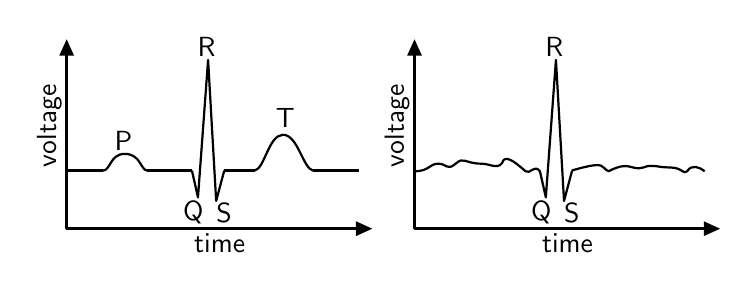
\begin{tikzpicture}[line join=round, xscale=0.555, yscale=0.48, >={Stealth[inset=0pt,length=6.0pt,angle'=45]}, every node/.style={font=\fontsize{10}{10}\sffamily}]
	\begin{scope}[x=2pt, y=-2pt]
		\draw[thick] (0,455.0021) -- (11.8345,455.0021);
	        \draw[thick] (11.8345,455.0021) .. controls (14.2834,454.8958) and
	          (14.1385,448.7114) .. (18.8842,448.7114) .. controls (24.2116,448.7114) and
	          (23.9695,454.8958) .. (26.3035,455.0021);
	        \draw[thick] (26.3035,455.0021) -- (40.7723,455.0021);
	        \draw[thick] (40.7723,455.0021) -- (42.7455,465.0645) -- (46.0339,413.3461)
	          -- (48.6647,466.4235) -- (51.2955,455.0021);
	        \draw[thick] (51.2955,455.0021) -- (61.1605,455.0021);
	        \draw[thick] (61.1605,455.0021) .. controls (64.4487,454.3298) and
	          (65.7118,441.6860) .. (70.3679,441.5241) .. controls (75.2428,441.3542) and
	          (76.9447,454.3301) .. (80.2329,455.0021);
	        % \draw[]  (80.2329,455.0021) .. controls (81.4852,455.0021) and
	         %  (82.2677,452.8462) .. (84.1792,452.9863) .. controls (85.8717,453.1101) and
	         % (86.4830,455.0021) .. (87.4678,455.0021);
	        \draw[thick] (80.1678,455.0021) -- (95,455.0021);
	\end{scope}
	\draw[very thick, <->] (0,-28.5) -- (0,-33.52) -- (7,-33.52);
	\node[] at (1.3,-31.2) {P};
	\node[] at (2.9,-33.1) {Q};
	\node[] at (3.2,-28.7) {R};
	\node[] at (3.6,-33.1) {S};
	\node[] at (5,-30.6) {T};
	\node[] at (3.5,-33.91) {time};
	\node[rotate=90] at (-0.4,-30.8) {voltage};
	\begin{scope}[xshift=9.5cm, shift={(-1.54,0)}]
		\begin{scope}[x=2pt, y=-2pt]
			
			\draw[thick] (40.7723,455.0021) -- (42.7455,465.0645) -- (46.0339,413.3461)
			  -- (48.6647,466.4235) -- (51.2955,455.0021);
			% \draw[thick] (51.2955,455.0021) -- (61.1605,455.0021);
			% \draw[thick] (61.1605,455.0021) .. controls (64.4487,454.3298) and
			  (65.7118,441.686) .. (70.3679,441.5241) .. controls (75.2428,441.3542) and
			  (76.9447,454.3301) .. (80.2329,455.0021);
			% \draw[]  (80.2329,455.0021) .. controls (81.4852,455.0021) and
			 %  (82.2677,452.8462) .. (84.1792,452.9863) .. controls (85.8717,453.1101) and
			 % (86.4830,455.0021) .. (87.4678,455.0021);
			% \draw[thick] (80.1678,455.0021) -- (95,455.0021);
		\end{scope}
	    \draw[very thick, <->] (0,-28.5) -- (0,-33.52) -- (7,-33.52);
    	\node[] at (2.9,-33.1) {Q};
    	\node[] at (3.2,-28.7) {R};
    	\node[] at (3.6,-33.1) {S};
	    \node[] at (3.5,-33.91) {time};
		\node[rotate=90] at (-0.4,-30.8) {voltage};
	\end{scope}
	\begin{scope}[xshift=-0.5cm]
	    \draw[thick] (8.46,-32) .. controls (8.8,-32) and (8.8,-31.8) .. (9,-31.8) .. controls (9.2,-31.8) and (9.2,-32) .. (9.4,-31.8) .. controls (9.6,-31.6) and (9.6,-31.8) .. (10,-31.8) .. controls (10.2,-31.8) and (10.4,-32) .. (10.5,-31.7) .. controls (10.6,-31.6) and (10.8,-31.8) .. (11,-32) .. controls (11.1,-32.1) and (11.2,-31.8) .. (11.33,-32);
	    \draw[thick] (12.06,-31.98) .. controls (12.9,-31.7) and (12.7,-31.9) .. (12.9,-32) .. controls (13.4,-31.7) and (13.4,-32) .. (13.7,-31.9) .. controls (13.9,-31.8) and (14,-31.9) .. (14.3,-31.9) .. controls (14.6,-31.9) and (14.6,-32.1) .. (14.7,-32) .. controls (14.8,-31.8) and (15,-31.9) .. (15.1,-32);

	\end{scope}
\end{tikzpicture}
    \caption{Regular heart beat with QRS complex, P wave, and T wave on the left and atrial fibrillation on the right. AF can be detected by the noisy ECG at the P and T wave regions. Please note that this is only a theoretical illustration. Real ECGs of AF can be seen in the appendix.}
    \label{fig:beat}
\end{figure}
\begin{figure*}[!ht]
    \centering
    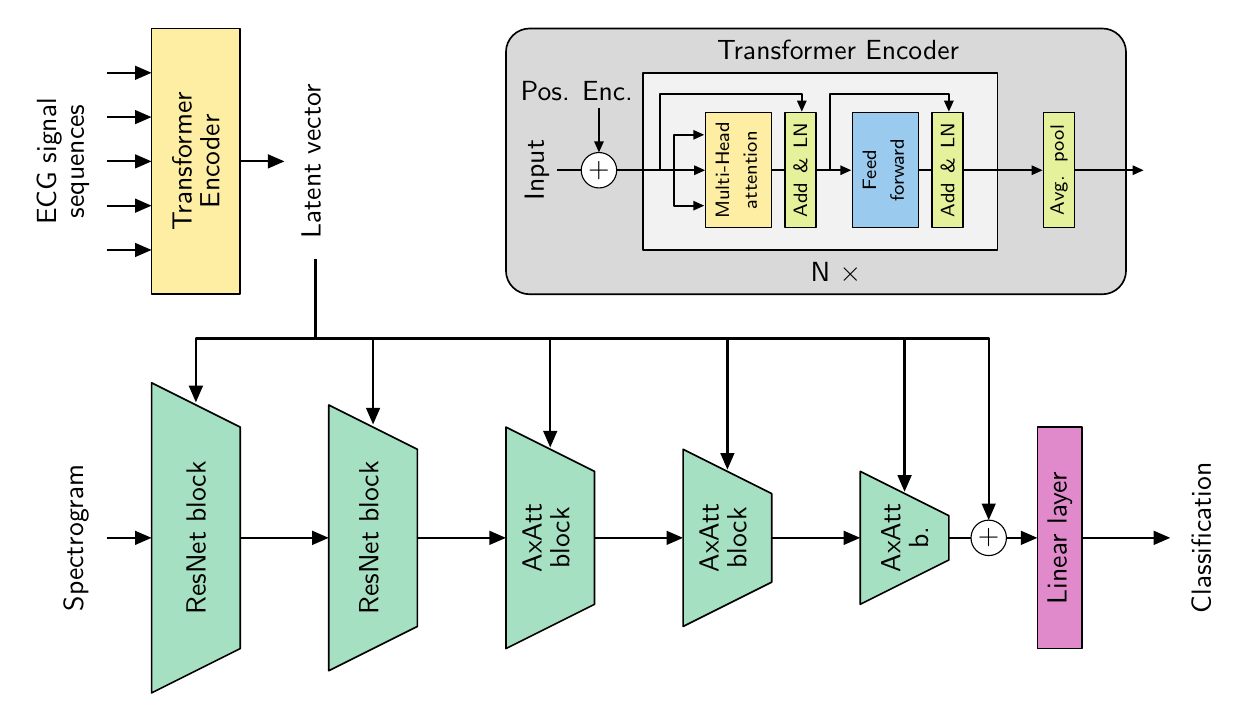
\begin{tikzpicture}[line join=round, >={Stealth[inset=0pt,length=6.0pt,angle'=45]}, every node/.style={font=\fontsize{10}{10}\sffamily}, scale=1.125]
	\draw[semithick, black, fill=tud6a!50]  (-3.5,3) rectangle (-2.5,0);
	\node[rotate=90, align=center, text width=2.25cm] at (-3,1.5) {Transformer Encoder};
	\node[rotate=90, align=center, text width=2.25cm] at (-4.5,1.5) {ECG signal sequences};
	\draw[thick, ->] (-4,2.5) -- (-3.5,2.5);
	\draw[thick, ->] (-4,2) -- (-3.5,2);
	\draw[thick, ->] (-4,1.5) -- (-3.5,1.5);
	\draw[thick, ->] (-4,1) -- (-3.5,1);
	\draw[thick, ->] (-4,0.5) -- (-3.5,0.5);
	\draw[thick, ->] (-2.5,1.5) -- (-2,1.5);
	\node[rotate=90, align=center, text width=2.25cm] at (-1.7,1.5) {Latent vector};
	\draw[semithick, black, fill=tud3a!50] (-3.5,-1) -- (-2.5,-1.5) -- (-2.5,-4) -- (-3.5,-4.5) -- cycle;
	\node[rotate=90, align=center, text width=2.5cm] at (-3,-2.75) {ResNet block};
	\draw[semithick, black, fill=tud3a!50] (-1.5,-1.25) -- (-0.5,-1.75) -- (-0.5,-3.75) -- (-1.5,-4.25) -- cycle;
	\node[rotate=90, align=center, text width=2.25cm] at (-1.05,-2.75) {ResNet block};
	\draw[semithick, black, fill=tud3a!50] (0.5,-1.5) -- (1.5,-2) -- (1.5,-3.5) -- (0.5,-4) -- cycle;
	\node[rotate=90, align=center, text width=1.5cm] at (0.95,-2.75) {AxAtt block};
	\draw[semithick, black, fill=tud3a!50] (2.5,-1.75) -- (3.5,-2.25) -- (3.5,-3.25) -- (2.5,-3.75) -- cycle;
	\node[rotate=90, align=center, text width=1.5cm] at (2.95,-2.75) {AxAtt block};
	\draw[semithick, black, fill=tud3a!50] (4.5,-2) -- (5.5,-2.5) -- (5.5,-3) -- (4.5,-3.5) -- cycle;
	\node[rotate=90, align=center, text width=1.0cm] at (5,-2.75) {AxAtt b.};
	\draw[thick, ->] (-1.65,0.4) -- (-1.65,-0.5) -- (5,-0.5) -- (5,-2.23);
	\draw[thick, <-] (-3,-1.22) -- (-3,-0.5) -- (-1.65,-0.5);
	\draw[thick, <-] (3,-1.98) -- (3,-0.5);
	\draw[thick, <-] (1,-1.73) -- (1,-0.5);
	\draw[thick, <-] (-1,-1.47) -- (-1,-0.5);
	\draw[thick, ->] (-2.5,-2.75) -- (-1.5,-2.75);
	\draw[thick, ->] (-0.5,-2.75) -- (0.5,-2.75);
	\draw[thick, ->] (1.5,-2.75) -- (2.5,-2.75);
	\draw[thick, ->] (3.5,-2.75) -- (4.5,-2.75);
	\draw[thick, ->] (5.5,-2.75) -- (6.5,-2.75);
	\draw[fill=white] (5.95,-2.75) circle (0.2cm);
	\node at (5.95,-2.75) {$+$};
	\draw[thick, ->] (5,-0.5) -- (5.95,-0.5) -- (5.95,-2.55);
	\draw[semithick, black, fill=tud10a!50]  (6.5,-1.5) rectangle (7,-4);
	\node[rotate=90, align=center, text width=2.25cm] at (6.75,-2.75) {Linear layer};
	\draw[thick, ->] (7,-2.75) -- (8,-2.75);
	\node[rotate=90, align=center, text width=2.25cm] at (8.35,-2.75) {Classification};
	\draw[thick, ->] (-4,-2.75) -- (-3.5,-2.75);
	\node[rotate=90] at (-4.35,-2.75) {Spectrogram};
	\begin{scope}[xshift=1.5cm]
	    \draw[semithick, fill=gray!30, rounded corners=3mm]  (-1,3) rectangle (6,0);
    	\node[align=center, text width=5cm] at (2.75,2.76) {Transformer Encoder};
    	\node[rotate=90, align=center, text width=2.25cm] at (-0.65,1.4) {Input};
    	\draw[semithick, fill=gray!10] (0.55,2.5) rectangle (4.55,0.5);
    	\draw[thick, ->, >={Stealth[inset=0pt,length=4.0pt,angle'=45]}] (-0.425,1.4) -- (1.25,1.4);
    	\draw[fill=white] (0.05,1.4) circle (0.2cm);
    	\node at (0.05,1.4) {$+$};
    	\draw[thick, <-, >={Stealth[inset=0pt,length=4.0pt,angle'=45]}] (0.05,1.6) -- (0.05,2.1);
    	\node at (-0.2,2.3) {Pos. Enc.};
    	\draw[fill=tud6a!50]  (1.25,0.75) rectangle (2,2.05);
    	\node[rotate=90, align=center, text width=2.25cm] at (1.6,1.4) {\scriptsize{Multi-Head attention}};
    	\draw[fill=tud5a!50]  (2.15,0.75) rectangle (2.5,2.05);
    	\node[rotate=90, align=center, text width=2.25cm] at (2.325,1.4) {\scriptsize{Add \& LN}};
    	\draw[thick] (2,1.4) -- (2.15,1.4);
    	\draw[thick, ->, >={Stealth[inset=0pt,length=4.0pt,angle'=45]}] (0.9,1.4) -- (0.9,1.8) -- (1.24,1.8);
    	\draw[thick, ->, >={Stealth[inset=0pt,length=4.0pt,angle'=45]}] (0.9,1.4) -- (0.9,1) -- (1.24,1);
    	\draw[thick, ->, >={Stealth[inset=0pt,length=4.0pt,angle'=45]}] (0.74,1.4) -- (0.74,2.26) -- (2.34,2.26) -- (2.34,2.06);
    	\begin{scope}[shift={(1.66,0)}]
    		\draw[thick, ->, >={Stealth[inset=0pt,length=4.0pt,angle'=45]}] (1,1.4) -- (1,2.26) -- (2.34,2.26) -- (2.34,2.06);
    		\draw[fill=tud2a!50]  (1.25,0.75) rectangle (2,2.05);
    		\node[rotate=90, align=center, text width=1.0cm] at (1.6,1.4) {\scriptsize{Feed forward}};
    		\draw[fill=tud5a!50]  (2.15,0.75) rectangle (2.5,2.05);
    		\node[rotate=90, align=center, text width=2.25cm] at (2.325,1.4) {\scriptsize{Add \& LN}};
    		\draw[thick] (2,1.4) -- (2.15,1.4);
    	\end{scope}
    	\draw[thick, ->, >={Stealth[inset=0pt,length=4.0pt,angle'=45]}] (2.5,1.4) -- (2.9,1.4);
    	\draw[thick, ->, >={Stealth[inset=0pt,length=4.0pt,angle'=45]}] (4.16,1.4) -- (5.06,1.4);
    	\draw[fill=tud5a!50]  (5.07,0.75) rectangle (5.42,2.05);
    	\node[rotate=90, align=center, text width=2.25cm] at (5.245,1.4) {\scriptsize{Avg. pool}};
    	\draw[thick, ->, >={Stealth[inset=0pt,length=4.0pt,angle'=45]}] (5.42,1.4) -- (6.2,1.4);
    	\node[align=center, text width=2.25cm] at (2.725,0.24) {N $\times$};
	\end{scope}
\end{tikzpicture}
    \caption{ECG-DualNet++ architecture with spectrogram and ECG signal as inputs. The ECG signal sequence gets encoded by a Transformer encoder to a single latent vector. The spectrogram is encoded by multiple 2D blocks. The first two blocks are standard ResNet like blocks and the following three blocks are Axial-Attention blocks. All blocks of the spectrogram encoder utilize the latent vector by conditional batch normalization. Transformer encoder \cite{Vaswani2017} architecture shown in the top right.}
    \label{fig:ecg_dual_net}
\end{figure*}
\indent In this study, we propose a novel deep learning approach for classifying AF in single-lead ECG recordings with variable lengths. Our novel deep learning approach ECG-DualNet utilized both input data for the time and frequency domain, enabling the network to learn features in both domains. The proposed ECG-DualNet surpasses the classification accuracy of recent convolutional neural network (CNN) approaches which only utilizes input data from the frequency domain \cite{Zihlmann2017}.



    \section{Method}

\subsection{ECG-DualNet}
\begin{frame}{Method}
\framesubtitle{ECG-DualNet(++)}
    \begin{figure}[!ht]
        \centering
        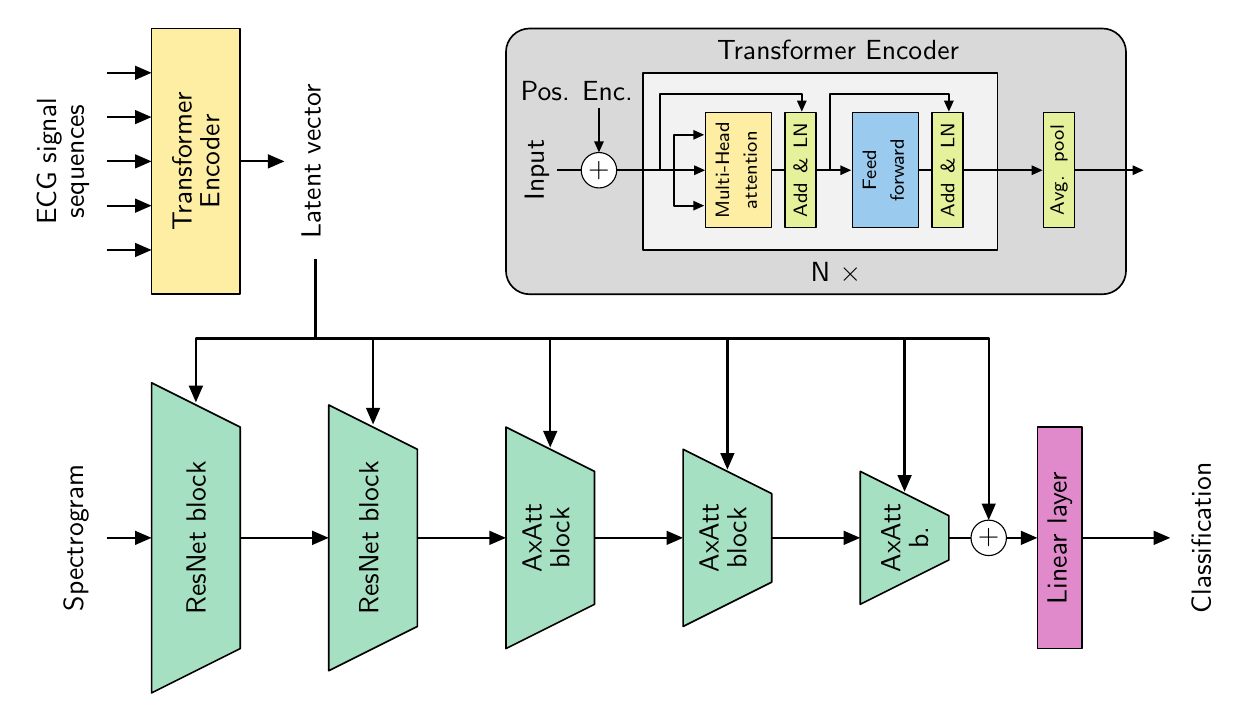
\begin{tikzpicture}[line join=round, >={Stealth[inset=0pt,length=6.0pt,angle'=45]}, every node/.style={font=\fontsize{10}{10}\sffamily}, scale=1.125]
	\draw[semithick, black, fill=tud6a!50]  (-3.5,3) rectangle (-2.5,0);
	\node[rotate=90, align=center, text width=2.25cm] at (-3,1.5) {Transformer Encoder};
	\node[rotate=90, align=center, text width=2.25cm] at (-4.5,1.5) {ECG signal sequences};
	\draw[thick, ->] (-4,2.5) -- (-3.5,2.5);
	\draw[thick, ->] (-4,2) -- (-3.5,2);
	\draw[thick, ->] (-4,1.5) -- (-3.5,1.5);
	\draw[thick, ->] (-4,1) -- (-3.5,1);
	\draw[thick, ->] (-4,0.5) -- (-3.5,0.5);
	\draw[thick, ->] (-2.5,1.5) -- (-2,1.5);
	\node[rotate=90, align=center, text width=2.25cm] at (-1.7,1.5) {Latent vector};
	\draw[semithick, black, fill=tud3a!50] (-3.5,-1) -- (-2.5,-1.5) -- (-2.5,-4) -- (-3.5,-4.5) -- cycle;
	\node[rotate=90, align=center, text width=2.5cm] at (-3,-2.75) {ResNet block};
	\draw[semithick, black, fill=tud3a!50] (-1.5,-1.25) -- (-0.5,-1.75) -- (-0.5,-3.75) -- (-1.5,-4.25) -- cycle;
	\node[rotate=90, align=center, text width=2.25cm] at (-1.05,-2.75) {ResNet block};
	\draw[semithick, black, fill=tud3a!50] (0.5,-1.5) -- (1.5,-2) -- (1.5,-3.5) -- (0.5,-4) -- cycle;
	\node[rotate=90, align=center, text width=1.5cm] at (0.95,-2.75) {AxAtt block};
	\draw[semithick, black, fill=tud3a!50] (2.5,-1.75) -- (3.5,-2.25) -- (3.5,-3.25) -- (2.5,-3.75) -- cycle;
	\node[rotate=90, align=center, text width=1.5cm] at (2.95,-2.75) {AxAtt block};
	\draw[semithick, black, fill=tud3a!50] (4.5,-2) -- (5.5,-2.5) -- (5.5,-3) -- (4.5,-3.5) -- cycle;
	\node[rotate=90, align=center, text width=1.0cm] at (5,-2.75) {AxAtt b.};
	\draw[thick, ->] (-1.65,0.4) -- (-1.65,-0.5) -- (5,-0.5) -- (5,-2.23);
	\draw[thick, <-] (-3,-1.22) -- (-3,-0.5) -- (-1.65,-0.5);
	\draw[thick, <-] (3,-1.98) -- (3,-0.5);
	\draw[thick, <-] (1,-1.73) -- (1,-0.5);
	\draw[thick, <-] (-1,-1.47) -- (-1,-0.5);
	\draw[thick, ->] (-2.5,-2.75) -- (-1.5,-2.75);
	\draw[thick, ->] (-0.5,-2.75) -- (0.5,-2.75);
	\draw[thick, ->] (1.5,-2.75) -- (2.5,-2.75);
	\draw[thick, ->] (3.5,-2.75) -- (4.5,-2.75);
	\draw[thick, ->] (5.5,-2.75) -- (6.5,-2.75);
	\draw[fill=white] (5.95,-2.75) circle (0.2cm);
	\node at (5.95,-2.75) {$+$};
	\draw[thick, ->] (5,-0.5) -- (5.95,-0.5) -- (5.95,-2.55);
	\draw[semithick, black, fill=tud10a!50]  (6.5,-1.5) rectangle (7,-4);
	\node[rotate=90, align=center, text width=2.25cm] at (6.75,-2.75) {Linear layer};
	\draw[thick, ->] (7,-2.75) -- (8,-2.75);
	\node[rotate=90, align=center, text width=2.25cm] at (8.35,-2.75) {Classification};
	\draw[thick, ->] (-4,-2.75) -- (-3.5,-2.75);
	\node[rotate=90] at (-4.35,-2.75) {Spectrogram};
	\begin{scope}[xshift=1.5cm]
	    \draw[semithick, fill=gray!30, rounded corners=3mm]  (-1,3) rectangle (6,0);
    	\node[align=center, text width=5cm] at (2.75,2.76) {Transformer Encoder};
    	\node[rotate=90, align=center, text width=2.25cm] at (-0.65,1.4) {Input};
    	\draw[semithick, fill=gray!10] (0.55,2.5) rectangle (4.55,0.5);
    	\draw[thick, ->, >={Stealth[inset=0pt,length=4.0pt,angle'=45]}] (-0.425,1.4) -- (1.25,1.4);
    	\draw[fill=white] (0.05,1.4) circle (0.2cm);
    	\node at (0.05,1.4) {$+$};
    	\draw[thick, <-, >={Stealth[inset=0pt,length=4.0pt,angle'=45]}] (0.05,1.6) -- (0.05,2.1);
    	\node at (-0.2,2.3) {Pos. Enc.};
    	\draw[fill=tud6a!50]  (1.25,0.75) rectangle (2,2.05);
    	\node[rotate=90, align=center, text width=2.25cm] at (1.6,1.4) {\scriptsize{Multi-Head attention}};
    	\draw[fill=tud5a!50]  (2.15,0.75) rectangle (2.5,2.05);
    	\node[rotate=90, align=center, text width=2.25cm] at (2.325,1.4) {\scriptsize{Add \& LN}};
    	\draw[thick] (2,1.4) -- (2.15,1.4);
    	\draw[thick, ->, >={Stealth[inset=0pt,length=4.0pt,angle'=45]}] (0.9,1.4) -- (0.9,1.8) -- (1.24,1.8);
    	\draw[thick, ->, >={Stealth[inset=0pt,length=4.0pt,angle'=45]}] (0.9,1.4) -- (0.9,1) -- (1.24,1);
    	\draw[thick, ->, >={Stealth[inset=0pt,length=4.0pt,angle'=45]}] (0.74,1.4) -- (0.74,2.26) -- (2.34,2.26) -- (2.34,2.06);
    	\begin{scope}[shift={(1.66,0)}]
    		\draw[thick, ->, >={Stealth[inset=0pt,length=4.0pt,angle'=45]}] (1,1.4) -- (1,2.26) -- (2.34,2.26) -- (2.34,2.06);
    		\draw[fill=tud2a!50]  (1.25,0.75) rectangle (2,2.05);
    		\node[rotate=90, align=center, text width=1.0cm] at (1.6,1.4) {\scriptsize{Feed forward}};
    		\draw[fill=tud5a!50]  (2.15,0.75) rectangle (2.5,2.05);
    		\node[rotate=90, align=center, text width=2.25cm] at (2.325,1.4) {\scriptsize{Add \& LN}};
    		\draw[thick] (2,1.4) -- (2.15,1.4);
    	\end{scope}
    	\draw[thick, ->, >={Stealth[inset=0pt,length=4.0pt,angle'=45]}] (2.5,1.4) -- (2.9,1.4);
    	\draw[thick, ->, >={Stealth[inset=0pt,length=4.0pt,angle'=45]}] (4.16,1.4) -- (5.06,1.4);
    	\draw[fill=tud5a!50]  (5.07,0.75) rectangle (5.42,2.05);
    	\node[rotate=90, align=center, text width=2.25cm] at (5.245,1.4) {\scriptsize{Avg. pool}};
    	\draw[thick, ->, >={Stealth[inset=0pt,length=4.0pt,angle'=45]}] (5.42,1.4) -- (6.2,1.4);
    	\node[align=center, text width=2.25cm] at (2.725,0.24) {N $\times$};
	\end{scope}
\end{tikzpicture}
        \caption{ECG-DualNet++ architecture with signal and spectrogram encoder}
        \label{fig:ecg_dual_net}
    \end{figure}
    \begin{textblock*}{3cm}(11.8cm, 3cm)
        \raggedright
        \cite{Vaswani2017}
        \cite{Wang2020}
        \cite{Dosovitskiy2020}
        \cite{De2017}
    \end{textblock*}
\end{frame}

\subsection{Augmentation Pipeline}
\begin{frame}{Method}
\framesubtitle{Augmentation Pipeline}
    \vspace{-0.251cm}
    \begin{figure}[!ht]
        \setlength{\figH}{4.5cm}
        \setlength{\figW}{0.33\textwidth}
        \centering
        % This file was created by tikzplotlib v0.9.6.
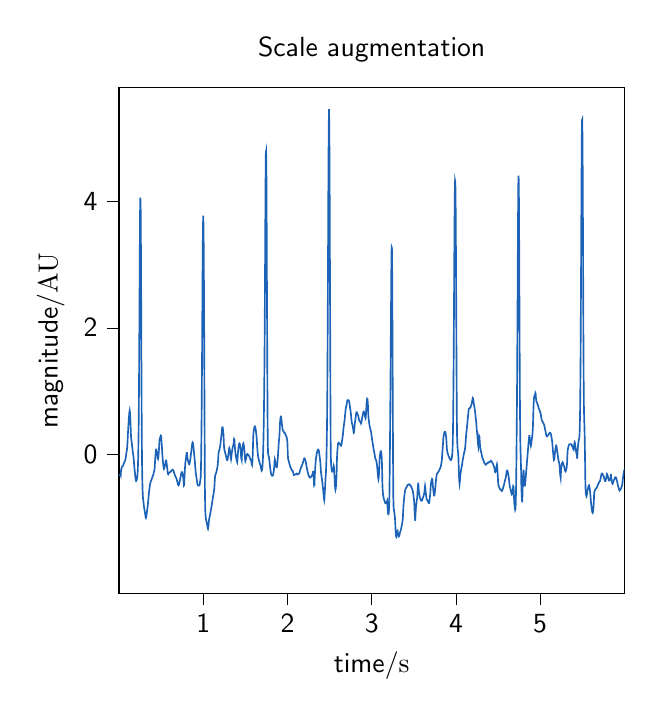
\begin{tikzpicture}
\pgfplotsset{
   every axis/.append style={
		font=\fontsize{10}{10}\sffamily},
	every non boxed x axis/.append style={
		x axis line style={->}
	},
	every non boxed y axis/.append style={
		y axis line style={->}
	},
	every non boxed z axis/.append style={
		z axis line style={->}
	}
}
\begin{axis}[
height=\figH,
tick align=outside,
tick pos=left,
width=\figW,
x grid style={white!69.0196078431373!black},
xlabel={time/$\si{\second}$},
xmin=0, xmax=6,
xtick style={color=black},
y grid style={white!69.0196078431373!black},
ylabel={magnitude/\si{AU}},
ymin=-2.19102610318908, ymax=5.78890501260757,
ytick style={color=black},
ytick = {0, 2, 4},
yticklabels = {0, 2, 4},
xtick = {1, 2, 3, 4, 5},
xticklabels = {1, 2, 3, 4, 5},
title = {Scale augmentation},
]
\addplot [semithick, tud1b]
table {%
0 -0.323440223932266
0.00333333341404796 -0.329041212797165
0.00666666682809591 -0.329041212797165
0.00999999977648258 -0.323440223932266
0.0133333336561918 -0.31783926486969
0.0166666675359011 -0.31783926486969
0.0199999995529652 -0.329041212797165
0.0233333334326744 -0.267430454492569
0.0266666673123837 -0.233824595808983
0.0299999993294477 -0.217021659016609
0.0333333350718021 -0.205819711089134
0.0366666652262211 -0.194617763161659
0.0399999991059303 -0.183415800333023
0.0433333329856396 -0.183415800333023
0.0466666668653488 -0.177814826369286
0.0500000007450581 -0.172213852405548
0.0533333346247673 -0.161011889576912
0.0566666685044765 -0.144208967685699
0.0599999986588955 -0.133007019758224
0.0633333325386047 -0.121805064380169
0.0666666701436043 -0.110603109002113
0.0700000002980232 -0.105002135038376
0.0733333304524422 -0.0938001871109009
0.0766666680574417 -0.0769972428679466
0.0799999982118607 -0.0489923655986786
0.0833333358168602 -0.02098748087883
0.0866666659712791 0.0126183768734336
0.0900000035762787 0.0406232587993145
0.0933333337306976 0.0686281397938728
0.0966666638851166 0.107834972441196
0.100000001490116 0.169445708394051
0.103333331644535 0.259061336517334
0.106666669249535 0.34307599067688
0.109999999403954 0.421489685773849
0.113333337008953 0.494302362203598
0.116666667163372 0.567115068435669
0.119999997317791 0.623124837875366
0.123333334922791 0.673533618450165
0.126666665077209 0.695937514305115
0.129999995231628 0.667932629585266
0.133333340287209 0.600720942020416
0.136666670441628 0.499903351068497
0.140000000596046 0.359878927469254
0.143333330750465 0.275864243507385
0.146666660904884 0.236657425761223
0.150000005960464 0.203051567077637
0.153333336114883 0.163844749331474
0.156666666269302 0.12463790178299
0.159999996423721 0.0854310765862465
0.16333332657814 0.046224232763052
0.16666667163372 0.0126183768734336
0.170000001788139 -0.0153865050524473
0.173333331942558 -0.0545933432877064
0.176666662096977 -0.0994011536240578
0.180000007152557 -0.161011889576912
0.183333337306976 -0.217021659016609
0.186666667461395 -0.256228506565094
0.189999997615814 -0.301036328077316
0.193333327770233 -0.345844149589539
0.196666672825813 -0.38505095243454
0.200000002980232 -0.40745484828949
0.203333333134651 -0.418656796216965
0.20666666328907 -0.413055837154388
0.209999993443489 -0.401853889226913
0.213333338499069 -0.379449963569641
0.216666668653488 -0.351445108652115
0.219999998807907 -0.312238276004791
0.223333328962326 -0.23942556977272
0.226666674017906 -0.0994011536240578
0.230000004172325 0.102233998477459
0.233333334326744 0.432691633701324
0.236666664481163 0.925577521324158
0.239999994635582 1.58649277687073
0.243333339691162 2.37062954902649
0.246666669845581 3.17717003822327
0.25 3.83248424530029
0.253333330154419 4.05652332305908
0.256666660308838 3.98371052742004
0.259999990463257 3.40120911598206
0.263333320617676 2.40423536300659
0.266666680574417 1.31764590740204
0.270000010728836 0.432691633701324
0.273333340883255 -0.116204082965851
0.276666671037674 -0.390651911497116
0.280000001192093 -0.55868124961853
0.283333331346512 -0.659498751163483
0.286666661500931 -0.704306602478027
0.28999999165535 -0.743513464927673
0.293333321809769 -0.782720327377319
0.296666651964188 -0.821927130222321
0.300000011920929 -0.849932014942169
0.303333342075348 -0.877936899662018
0.306666672229767 -0.900340795516968
0.310000002384186 -0.933946669101715
0.313333332538605 -0.967552542686462
0.316666662693024 -0.989956438541412
0.319999992847443 -1.00115835666656
0.323333323001862 -0.989956438541412
0.326666653156281 -0.961951613426208
0.330000013113022 -0.922744691371918
0.333333343267441 -0.889138877391815
0.33666667342186 -0.855533003807068
0.340000003576279 -0.821927130222321
0.343333333730698 -0.782720327377319
0.346666663885117 -0.737912476062775
0.349999994039536 -0.687503695487976
0.353333324193954 -0.637094855308533
0.356666654348373 -0.592287123203278
0.360000014305115 -0.553080201148987
0.363333344459534 -0.519474387168884
0.366666674613953 -0.485868513584137
0.370000004768372 -0.463464587926865
0.373333334922791 -0.441060721874237
0.376666665077209 -0.429858773946762
0.379999995231628 -0.418656796216965
0.383333325386047 -0.40745484828949
0.386666655540466 -0.396252900362015
0.389999985694885 -0.38505095243454
0.393333345651627 -0.368248015642166
0.396666675806046 -0.357046097517014
0.400000005960464 -0.345844149589539
0.403333336114883 -0.334642171859741
0.406666666269302 -0.31783926486969
0.409999996423721 -0.301036328077316
0.41333332657814 -0.284233391284943
0.416666656732559 -0.267430454492569
0.419999986886978 -0.250627517700195
0.423333346843719 -0.217021659016609
0.426666676998138 -0.138607993721962
0.430000007152557 -0.0657952949404716
0.433333337306976 -0.00418455293402076
0.436666667461395 0.046224232763052
0.439999997615814 0.0798300951719284
0.443333327770233 0.0798300951719284
0.446666657924652 0.0518252104520798
0.449999988079071 0.0238203294575214
0.453333348035812 -0.00418455293402076
0.456666678190231 -0.0321894362568855
0.46000000834465 -0.0601943209767342
0.463333338499069 -0.0713962689042091
0.466666668653488 -0.0545933432877064
0.469999998807907 -0.00418455293402076
0.473333328962326 0.0574261881411076
0.476666659116745 0.12463790178299
0.479999989271164 0.214253515005112
0.483333319425583 0.247859388589859
0.486666679382324 0.259061336517334
0.490000009536743 0.270263284444809
0.493333339691162 0.287066221237183
0.496666669845581 0.298268169164658
0.5 0.292667180299759
0.503333330154419 0.242258414626122
0.506666660308838 0.175046682357788
0.509999990463257 0.113435953855515
0.513333320617676 0.0294213071465492
0.516666650772095 -0.037790410220623
0.519999980926514 -0.0881991982460022
0.523333311080933 -0.133007019758224
0.526666641235352 -0.177814826369286
0.529999971389771 -0.211420685052872
0.533333361148834 -0.228223621845245
0.536666691303253 -0.222622647881508
0.540000021457672 -0.205819711089134
0.543333351612091 -0.183415800333023
0.54666668176651 -0.166612878441811
0.550000011920929 -0.144208967685699
0.553333342075348 -0.116204082965851
0.556666672229767 -0.0938001871109009
0.560000002384186 -0.0938001871109009
0.563333332538605 -0.116204082965851
0.566666662693024 -0.149809941649437
0.569999992847443 -0.189016774296761
0.573333323001862 -0.222622647881508
0.576666653156281 -0.267430454492569
0.579999983310699 -0.306637287139893
0.583333313465118 -0.312238276004791
0.586666643619537 -0.301036328077316
0.589999973773956 -0.295435339212418
0.593333303928375 -0.289834380149841
0.596666693687439 -0.289834380149841
0.600000023841858 -0.284233391284943
0.603333353996277 -0.278632402420044
0.606666684150696 -0.278632402420044
0.610000014305115 -0.273031443357468
0.613333344459534 -0.273031443357468
0.616666674613953 -0.267430454492569
0.620000004768372 -0.261829495429993
0.623333334922791 -0.250627517700195
0.626666665077209 -0.250627517700195
0.629999995231628 -0.245026543736458
0.633333325386047 -0.250627517700195
0.636666655540466 -0.250627517700195
0.639999985694885 -0.245026543736458
0.643333315849304 -0.250627517700195
0.646666646003723 -0.256228506565094
0.649999976158142 -0.267430454492569
0.653333306312561 -0.284233391284943
0.656666696071625 -0.295435339212418
0.660000026226044 -0.312238276004791
0.663333356380463 -0.323440223932266
0.666666686534882 -0.334642171859741
0.670000016689301 -0.345844149589539
0.673333346843719 -0.357046097517014
0.676666676998138 -0.362647026777267
0.680000007152557 -0.373849004507065
0.683333337306976 -0.38505095243454
0.686666667461395 -0.396252900362015
0.689999997615814 -0.418656796216965
0.693333327770233 -0.435459733009338
0.696666657924652 -0.457863658666611
0.699999988079071 -0.47466653585434
0.70333331823349 -0.480267524719238
0.706666648387909 -0.485868513584137
0.709999978542328 -0.480267524719238
0.713333308696747 -0.469065576791763
0.716666638851166 -0.452262669801712
0.720000028610229 -0.429858773946762
0.723333358764648 -0.40745484828949
0.726666688919067 -0.38505095243454
0.730000019073486 -0.362647026777267
0.733333349227905 -0.34024316072464
0.736666679382324 -0.312238276004791
0.740000009536743 -0.295435339212418
0.743333339691162 -0.278632402420044
0.746666669845581 -0.278632402420044
0.75 -0.278632402420044
0.753333330154419 -0.295435339212418
0.756666660308838 -0.31783926486969
0.759999990463257 -0.345844149589539
0.763333320617676 -0.373849004507065
0.766666650772095 -0.418656796216965
0.769999980926514 -0.491469472646713
0.773333311080933 -0.485868513584137
0.776666641235352 -0.379449963569641
0.779999971389771 -0.289834380149841
0.783333361148834 -0.211420685052872
0.786666691303253 -0.149809941649437
0.790000021457672 -0.105002135038376
0.793333351612091 -0.0769972428679466
0.79666668176651 -0.0433913879096508
0.800000011920929 -0.00418455293402076
0.803333342075348 0.0238203294575214
0.806666672229767 0.0238203294575214
0.810000002384186 -0.0153865050524473
0.813333332538605 -0.0601943209767342
0.816666662693024 -0.0825982242822647
0.819999992847443 -0.0994011536240578
0.823333323001862 -0.121805064380169
0.826666653156281 -0.138607993721962
0.829999983310699 -0.149809941649437
0.833333313465118 -0.155410915613174
0.836666643619537 -0.149809941649437
0.839999973773956 -0.133007019758224
0.843333303928375 -0.105002135038376
0.846666693687439 -0.0769972428679466
0.850000023841858 -0.0433913879096508
0.853333353996277 -0.00418455293402076
0.856666684150696 0.0294213071465492
0.860000014305115 0.0686281397938728
0.863333344459534 0.107834972441196
0.866666674613953 0.147041812539101
0.870000004768372 0.175046682357788
0.873333334922791 0.191849619150162
0.876666665077209 0.186248630285263
0.879999995231628 0.163844749331474
0.883333325386047 0.130238875746727
0.886666655540466 0.0854310765862465
0.889999985694885 0.0406232587993145
0.893333315849304 -0.00418455293402076
0.896666646003723 -0.0545933432877064
0.899999976158142 -0.105002135038376
0.903333306312561 -0.161011889576912
0.906666696071625 -0.217021659016609
0.910000026226044 -0.267430454492569
0.913333356380463 -0.306637287139893
0.916666686534882 -0.334642171859741
0.920000016689301 -0.362647026777267
0.923333346843719 -0.396252900362015
0.926666676998138 -0.429858773946762
0.930000007152557 -0.457863658666611
0.933333337306976 -0.47466653585434
0.936666667461395 -0.485868513584137
0.939999997615814 -0.491469472646713
0.943333327770233 -0.491469472646713
0.946666657924652 -0.491469472646713
0.949999988079071 -0.491469472646713
0.95333331823349 -0.491469472646713
0.956666648387909 -0.480267524719238
0.959999978542328 -0.457863658666611
0.963333308696747 -0.424257785081863
0.966666638851166 -0.390651911497116
0.970000028610229 -0.362647026777267
0.973333358764648 -0.211420685052872
0.976666688919067 0.0742291212081909
0.980000019073486 0.477499425411224
0.983333349227905 1.0095921754837
0.986666679382324 1.67050743103027
0.990000009536743 2.4154372215271
0.993333339691162 3.12116003036499
0.996666669845581 3.60284399986267
1 3.77087354660034
1.00333333015442 3.61964702606201
1.00666666030884 3.14916515350342
1.00999999046326 2.28101396560669
1.01333332061768 1.27283811569214
1.01666665077209 0.264662325382233
1.01999998092651 -0.541878283023834
1.02333331108093 -0.855533003807068
1.02666664123535 -0.950749635696411
1.02999997138977 -1.00115835666656
1.03333330154419 -1.02916324138641
1.03666663169861 -1.05156719684601
1.03999996185303 -1.06837010383606
1.04333329200745 -1.08517301082611
1.04666662216187 -1.10757696628571
1.04999995231628 -1.13558185100555
1.0533332824707 -1.1635867357254
1.05666661262512 -1.17478859424591
1.05999994277954 -1.15798580646515
1.06333339214325 -1.11317789554596
1.06666672229767 -1.05716812610626
1.07000005245209 -1.02356231212616
1.07333338260651 -1.00115835666656
1.07666671276093 -0.978754460811615
1.08000004291534 -0.961951613426208
1.08333337306976 -0.933946669101715
1.08666670322418 -0.911542773246765
1.0900000333786 -0.883537888526917
1.09333336353302 -0.861133992671967
1.09666669368744 -0.833129107952118
1.10000002384186 -0.810725152492523
1.10333335399628 -0.782720327377319
1.1066666841507 -0.754715383052826
1.11000001430511 -0.721109569072723
1.11333334445953 -0.69310462474823
1.11666667461395 -0.659498751163483
1.12000000476837 -0.637094855308533
1.12333333492279 -0.614690959453583
1.12666666507721 -0.586686074733734
1.12999999523163 -0.55868124961853
1.13333332538605 -0.497070461511612
1.13666665554047 -0.413055837154388
1.13999998569489 -0.357046097517014
1.1433333158493 -0.329041212797165
1.14666664600372 -0.312238276004791
1.14999997615814 -0.301036328077316
1.15333330631256 -0.289834380149841
1.15666663646698 -0.273031443357468
1.1599999666214 -0.256228506565094
1.16333329677582 -0.233824595808983
1.16666662693024 -0.211420685052872
1.16999995708466 -0.183415800333023
1.17333328723907 -0.144208967685699
1.17666661739349 -0.0938001871109009
1.17999994754791 -0.0153865050524473
1.18333327770233 0.035022284835577
1.18666660785675 0.0518252104520798
1.19000005722046 0.0686281397938728
1.19333338737488 0.0798300951719284
1.1966667175293 0.102233998477459
1.20000004768372 0.12463790178299
1.20333337783813 0.152642786502838
1.20666670799255 0.191849619150162
1.21000003814697 0.236657425761223
1.21333336830139 0.275864243507385
1.21666669845581 0.309470117092133
1.22000002861023 0.354277938604355
1.22333335876465 0.404686748981476
1.22666668891907 0.432691633701324
1.23000001907349 0.432691633701324
1.23333334922791 0.410287737846375
1.23666667938232 0.371080905199051
1.24000000953674 0.326273053884506
1.24333333969116 0.236657425761223
1.24666666984558 0.12463790178299
1.25 0.0854310765862465
1.25333333015442 0.0630271658301353
1.25666666030884 0.046224232763052
1.25999999046326 0.0294213071465492
1.26333332061768 0.0126183768734336
1.26666665077209 -0.00418455293402076
1.26999998092651 -0.02098748087883
1.27333331108093 -0.037790410220623
1.27666664123535 -0.0601943209767342
1.27999997138977 -0.0825982242822647
1.28333330154419 -0.0881991982460022
1.28666663169861 -0.0881991982460022
1.28999996185303 -0.0713962689042091
1.29333329200745 -0.0433913879096508
1.29666662216187 -0.00978552922606468
1.29999995231628 0.0126183768734336
1.3033332824707 0.0518252104520798
1.30666661262512 0.0854310765862465
1.30999994277954 0.102233998477459
1.31333339214325 0.0910320430994034
1.31666672229767 0.0630271658301353
1.32000005245209 0.0294213071465492
1.32333338260651 -0.00418455293402076
1.32666671276093 -0.0545933432877064
1.33000004291534 -0.0769972428679466
1.33333337306976 -0.0489923655986786
1.33666670322418 0.00141642359085381
1.3400000333786 0.035022284835577
1.34333336353302 0.0630271658301353
1.34666669368744 0.0910320430994034
1.35000002384186 0.113435953855515
1.35333335399628 0.130238875746727
1.3566666841507 0.147041812539101
1.36000001430511 0.169445708394051
1.36333334445953 0.197450593113899
1.36666667461395 0.247859388589859
1.37000000476837 0.242258414626122
1.37333333492279 0.163844749331474
1.37666666507721 0.102233998477459
1.37999999523163 0.0518252104520798
1.38333332538605 0.00701740011572838
1.38666665554047 -0.02098748087883
1.38999998569489 -0.0433913879096508
1.3933333158493 -0.0601943209767342
1.39666664600372 -0.0825982242822647
1.39999997615814 -0.110603109002113
1.40333330631256 -0.121805064380169
1.40666663646698 -0.0825982242822647
1.4099999666214 -0.00418455293402076
1.41333329677582 0.0406232587993145
1.41666662693024 0.0798300951719284
1.41999995708466 0.119036927819252
1.42333328723907 0.152642786502838
1.42666661739349 0.169445708394051
1.42999994754791 0.175046682357788
1.43333327770233 0.169445708394051
1.43666660785675 0.152642786502838
1.44000005722046 0.130238875746727
1.44333338737488 0.0966330170631409
1.4466667175293 0.0294213071465492
1.45000004768372 -0.0433913879096508
1.45333337783813 -0.0713962689042091
1.45666670799255 -0.0881991982460022
1.46000003814697 -0.00978552922606468
1.46333336830139 0.0574261881411076
1.46666669845581 0.0966330170631409
1.47000002861023 0.135839864611626
1.47333335876465 0.163844749331474
1.47666668891907 0.175046682357788
1.48000001907349 0.163844749331474
1.48333334922791 0.130238875746727
1.48666667938232 0.0910320430994034
1.49000000953674 0.046224232763052
1.49333333969116 0.00141642359085381
1.49666666984558 -0.0713962689042091
1.5 -0.105002135038376
1.50333333015442 -0.0938001871109009
1.50666666030884 -0.0713962689042091
1.50999999046326 -0.0545933432877064
1.51333332061768 -0.037790410220623
1.51666665077209 -0.0153865050524473
1.51999998092651 0.00141642359085381
1.52333331108093 0.00701740011572838
1.52666664123535 0.00701740011572838
1.52999997138977 0.00141642359085381
1.53333330154419 -0.00418455293402076
1.53666663169861 -0.00978552922606468
1.53999996185303 -0.0153865050524473
1.54333329200745 -0.02098748087883
1.54666662216187 -0.0265884585678577
1.54999995231628 -0.037790410220623
1.5533332824707 -0.0545933432877064
1.55666661262512 -0.0657952949404716
1.55999994277954 -0.0769972428679466
1.56333339214325 -0.0825982242822647
1.56666672229767 -0.0938001871109009
1.57000005245209 -0.105002135038376
1.57333338260651 -0.127406045794487
1.57666671276093 -0.155410915613174
1.58000004291534 -0.166612878441811
1.58333337306976 -0.127406045794487
1.58666670322418 -0.037790410220623
1.5900000333786 0.0966330170631409
1.59333336353302 0.270263284444809
1.59666669368744 0.337475001811981
1.60000002384186 0.376681864261627
1.60333335399628 0.3990857899189
1.6066666841507 0.421489685773849
1.61000001430511 0.438292622566223
1.61333334445953 0.443893551826477
1.61666667461395 0.438292622566223
1.62000000476837 0.421489685773849
1.62333333492279 0.393484801054001
1.62666666507721 0.359878927469254
1.62999999523163 0.320672065019608
1.63333332538605 0.275864243507385
1.63666665554047 0.208652541041374
1.63999998569489 0.141440838575363
1.6433333158493 0.0742291212081909
1.64666664600372 0.0238203294575214
1.64999997615814 -0.00978552922606468
1.65333330631256 -0.0433913879096508
1.65666663646698 -0.0657952949404716
1.6599999666214 -0.0825982242822647
1.66333329677582 -0.0994011536240578
1.66666662693024 -0.116204082965851
1.66999995708466 -0.133007019758224
1.67333328723907 -0.144208967685699
1.67666661739349 -0.161011889576912
1.67999994754791 -0.172213852405548
1.68333327770233 -0.189016774296761
1.68666660785675 -0.217021659016609
1.69000005722046 -0.23942556977272
1.69333338737488 -0.256228506565094
1.6966667175293 -0.250627517700195
1.70000004768372 -0.228223621845245
1.70333337783813 -0.183415800333023
1.70666670799255 -0.121805064380169
1.71000003814697 -0.02098748087883
1.71333336830139 0.130238875746727
1.71666669845581 0.359878927469254
1.72000002861023 0.617523849010468
1.72333335876465 0.942380428314209
1.72666668891907 1.39045858383179
1.73000001907349 2.0009651184082
1.73333334922791 2.76269793510437
1.73666667938232 3.58604121208191
1.74000000953674 4.33657217025757
1.74333333969116 4.76784753799438
1.74666666984558 4.7902512550354
1.75 4.44859170913696
1.75333333015442 3.61964702606201
1.75666666030884 2.57226490974426
1.75999999046326 1.53048312664032
1.76333332061768 0.679134607315063
1.76666665077209 0.147041812539101
1.76999998092651 0.0182193517684937
1.77333331108093 -0.00978552922606468
1.77666664123535 -0.0265884585678577
1.77999997138977 -0.0433913879096508
1.78333330154419 -0.0769972428679466
1.78666663169861 -0.110603109002113
1.78999996185303 -0.155410915613174
1.79333329200745 -0.194617763161659
1.79666662216187 -0.228223621845245
1.79999995231628 -0.261829495429993
1.8033332824707 -0.289834380149841
1.80666661262512 -0.312238276004791
1.80999994277954 -0.323440223932266
1.81333339214325 -0.329041212797165
1.81666672229767 -0.334642171859741
1.82000005245209 -0.334642171859741
1.82333338260651 -0.334642171859741
1.82666671276093 -0.329041212797165
1.83000004291534 -0.31783926486969
1.83333337306976 -0.295435339212418
1.83666670322418 -0.267430454492569
1.8400000333786 -0.228223621845245
1.84333336353302 -0.189016774296761
1.84666669368744 -0.110603109002113
1.85000002384186 -0.0769972428679466
1.85333335399628 -0.0938001871109009
1.8566666841507 -0.133007019758224
1.86000001430511 -0.155410915613174
1.86333334445953 -0.172213852405548
1.86666667461395 -0.189016774296761
1.87000000476837 -0.200218737125397
1.87333333492279 -0.200218737125397
1.87666666507721 -0.177814826369286
1.87999999523163 -0.133007019758224
1.88333332538605 -0.0825982242822647
1.88666665554047 -0.0321894362568855
1.88999998569489 0.0294213071465492
1.8933333158493 0.107834972441196
1.89666664600372 0.186248630285263
1.89999997615814 0.231056451797485
1.90333330631256 0.270263284444809
1.90666663646698 0.348676949739456
1.9099999666214 0.460696488618851
1.91333329677582 0.533509194850922
1.91666662693024 0.572716057300568
1.91999995708466 0.600720942020416
1.92333328723907 0.600720942020416
1.92666661739349 0.572716057300568
1.92999994754791 0.527908205986023
1.93333327770233 0.488701373338699
1.93666660785675 0.443893551826477
1.94000005722046 0.415888726711273
1.94333338737488 0.393484801054001
1.9466667175293 0.376681864261627
1.95000004768372 0.371080905199051
1.95333337783813 0.365479916334152
1.95666670799255 0.359878927469254
1.96000003814697 0.348676949739456
1.96333336830139 0.34307599067688
1.96666669845581 0.337475001811981
1.97000002861023 0.337475001811981
1.97333335876465 0.326273053884506
1.97666668891907 0.315071105957031
1.98000001907349 0.303869128227234
1.98333334922791 0.292667180299759
1.98666667938232 0.281465232372284
1.99000000953674 0.270263284444809
1.99333333969116 0.253460347652435
1.99666666984558 0.231056451797485
2 0.175046682357788
2.00333333015442 0.0238203294575214
2.00666666030884 -0.0545933432877064
2.00999999046326 -0.0825982242822647
2.01333332061768 -0.0938001871109009
2.01666665077209 -0.110603109002113
2.01999998092651 -0.127406045794487
2.02333331108093 -0.144208967685699
2.02666664123535 -0.161011889576912
2.02999997138977 -0.177814826369286
2.03333330154419 -0.194617763161659
2.03666663169861 -0.205819711089134
2.03999996185303 -0.211420685052872
2.04333329200745 -0.222622647881508
2.04666662216187 -0.233824595808983
2.04999995231628 -0.245026543736458
2.0533332824707 -0.250627517700195
2.05666661262512 -0.256228506565094
2.05999994277954 -0.256228506565094
2.06333327293396 -0.261829495429993
2.06666660308838 -0.278632402420044
2.0699999332428 -0.295435339212418
2.07333326339722 -0.312238276004791
2.07666659355164 -0.323440223932266
2.07999992370605 -0.323440223932266
2.08333325386047 -0.31783926486969
2.08666658401489 -0.31783926486969
2.08999991416931 -0.31783926486969
2.09333324432373 -0.31783926486969
2.09666657447815 -0.31783926486969
2.09999990463257 -0.312238276004791
2.10333323478699 -0.306637287139893
2.10666656494141 -0.301036328077316
2.10999989509583 -0.301036328077316
2.11333322525024 -0.306637287139893
2.11666655540466 -0.306637287139893
2.11999988555908 -0.312238276004791
2.1233332157135 -0.306637287139893
2.1266667842865 -0.306637287139893
2.13000011444092 -0.306637287139893
2.13333344459534 -0.306637287139893
2.13666677474976 -0.301036328077316
2.14000010490417 -0.295435339212418
2.14333343505859 -0.284233391284943
2.14666676521301 -0.267430454492569
2.15000009536743 -0.245026543736458
2.15333342552185 -0.233824595808983
2.15666675567627 -0.222622647881508
2.16000008583069 -0.211420685052872
2.16333341598511 -0.200218737125397
2.16666674613953 -0.189016774296761
2.17000007629395 -0.177814826369286
2.17333340644836 -0.166612878441811
2.17666673660278 -0.155410915613174
2.1800000667572 -0.144208967685699
2.18333339691162 -0.133007019758224
2.18666672706604 -0.116204082965851
2.19000005722046 -0.0938001871109009
2.19333338737488 -0.0825982242822647
2.1966667175293 -0.0713962689042091
2.20000004768372 -0.0601943209767342
2.20333337783813 -0.0601943209767342
2.20666670799255 -0.0713962689042091
2.21000003814697 -0.0825982242822647
2.21333336830139 -0.0938001871109009
2.21666669845581 -0.110603109002113
2.22000002861023 -0.133007019758224
2.22333335876465 -0.161011889576912
2.22666668891907 -0.183415800333023
2.23000001907349 -0.211420685052872
2.23333334922791 -0.233824595808983
2.23666667938232 -0.256228506565094
2.24000000953674 -0.273031443357468
2.24333333969116 -0.289834380149841
2.24666666984558 -0.312238276004791
2.25 -0.323440223932266
2.25333333015442 -0.334642171859741
2.25666666030884 -0.345844149589539
2.25999999046326 -0.357046097517014
2.26333332061768 -0.362647026777267
2.26666665077209 -0.362647026777267
2.26999998092651 -0.362647026777267
2.27333331108093 -0.362647026777267
2.27666664123535 -0.362647026777267
2.27999997138977 -0.351445108652115
2.28333330154419 -0.345844149589539
2.28666663169861 -0.34024316072464
2.28999996185303 -0.334642171859741
2.29333329200745 -0.323440223932266
2.29666662216187 -0.31783926486969
2.29999995231628 -0.301036328077316
2.3033332824707 -0.273031443357468
2.30666661262512 -0.273031443357468
2.30999994277954 -0.345844149589539
2.31333327293396 -0.418656796216965
2.31666660308838 -0.491469472646713
2.3199999332428 -0.485868513584137
2.32333326339722 -0.379449963569641
2.32666659355164 -0.284233391284943
2.32999992370605 -0.205819711089134
2.33333325386047 -0.138607993721962
2.33666658401489 -0.0881991982460022
2.33999991416931 -0.0489923655986786
2.34333324432373 -0.02098748087883
2.34666657447815 0.00701740011572838
2.34999990463257 0.0294213071465492
2.35333323478699 0.0518252104520798
2.35666656494141 0.0630271658301353
2.35999989509583 0.0742291212081909
2.36333322525024 0.0798300951719284
2.36666655540466 0.0798300951719284
2.36999988555908 0.0686281397938728
2.3733332157135 0.0518252104520798
2.3766667842865 0.0238203294575214
2.38000011444092 -0.00978552922606468
2.38333344459534 -0.0433913879096508
2.38666677474976 -0.0825982242822647
2.39000010490417 -0.121805064380169
2.39333343505859 -0.189016774296761
2.39666676521301 -0.256228506565094
2.40000009536743 -0.301036328077316
2.40333342552185 -0.334642171859741
2.40666675567627 -0.368248015642166
2.41000008583069 -0.396252900362015
2.41333341598511 -0.435459733009338
2.41666674613953 -0.47466653585434
2.42000007629395 -0.513873398303986
2.42333340644836 -0.553080201148987
2.42666673660278 -0.597888052463531
2.4300000667572 -0.642695844173431
2.43333339691162 -0.698705613613129
2.43666672706604 -0.721109569072723
2.44000005722046 -0.681902647018433
2.44333338737488 -0.592287123203278
2.4466667175293 -0.513873398303986
2.45000004768372 -0.424257785081863
2.45333337783813 -0.345844149589539
2.45666670799255 -0.284233391284943
2.46000003814697 -0.177814826369286
2.46333336830139 -0.037790410220623
2.46666669845581 0.208652541041374
2.47000002861023 0.51670628786087
2.47333335876465 0.998390197753906
2.47666668891907 1.70411336421967
2.48000001907349 2.61707258224487
2.48333334922791 3.63645005226135
2.48666667938232 4.56621217727661
2.49000000953674 5.21032428741455
2.49333333969116 5.4511661529541
2.49666666984558 5.19912242889404
2.5 4.45979404449463
2.50333333015442 3.36200213432312
2.50666666030884 2.10178279876709
2.50999999046326 0.942380428314209
2.51333332061768 0.107834972441196
2.51666665077209 -0.116204082965851
2.51999998092651 -0.177814826369286
2.52333331108093 -0.222622647881508
2.52666664123535 -0.256228506565094
2.52999997138977 -0.267430454492569
2.53333330154419 -0.261829495429993
2.53666663169861 -0.256228506565094
2.53999996185303 -0.245026543736458
2.54333329200745 -0.233824595808983
2.54666662216187 -0.217021659016609
2.54999995231628 -0.183415800333023
2.5533332824707 -0.200218737125397
2.55666661262512 -0.312238276004791
2.55999994277954 -0.390651911497116
2.56333327293396 -0.469065576791763
2.56666660308838 -0.530676305294037
2.5699999332428 -0.55868124961853
2.57333326339722 -0.541878283023834
2.57666659355164 -0.491469472646713
2.57999992370605 -0.418656796216965
2.58333325386047 -0.31783926486969
2.58666658401489 -0.116204082965851
2.58999991416931 0.00701740011572838
2.59333324432373 0.0686281397938728
2.59666657447815 0.119036927819252
2.59999990463257 0.163844749331474
2.60333323478699 0.180647656321526
2.60666656494141 0.186248630285263
2.60999989509583 0.180647656321526
2.61333322525024 0.175046682357788
2.61666655540466 0.175046682357788
2.61999988555908 0.169445708394051
2.6233332157135 0.163844749331474
2.6266667842865 0.158243760466576
2.63000011444092 0.147041812539101
2.63333344459534 0.135839864611626
2.63666677474976 0.135839864611626
2.64000010490417 0.147041812539101
2.64333343505859 0.175046682357788
2.64666676521301 0.203051567077637
2.65000009536743 0.236657425761223
2.65333342552185 0.264662325382233
2.65666675567627 0.298268169164658
2.66000008583069 0.337475001811981
2.66333341598511 0.387883841991425
2.66666674613953 0.427090674638748
2.67000007629395 0.460696488618851
2.67333340644836 0.494302362203598
2.67666673660278 0.522307217121124
2.6800000667572 0.567115068435669
2.68333339691162 0.611922860145569
2.68666672706604 0.656730711460114
2.69000005722046 0.701538503170013
2.69333338737488 0.735144317150116
2.6966667175293 0.757548213005066
2.70000004768372 0.774351179599762
2.70333337783813 0.796755015850067
2.70666670799255 0.824759960174561
2.71000003814697 0.84716385602951
2.71333336830139 0.858365833759308
2.71666669845581 0.858365833759308
2.72000002861023 0.858365833759308
2.72333335876465 0.858365833759308
2.72666668891907 0.858365833759308
2.73000001907349 0.84716385602951
2.73333334922791 0.830360889434814
2.73666667938232 0.802356064319611
2.74000000953674 0.768750190734863
2.74333333969116 0.735144317150116
2.74666666984558 0.707139432430267
2.75 0.679134607315063
2.75333333015442 0.639927744865417
2.75666666030884 0.595119893550873
2.75999999046326 0.544711172580719
2.76333332061768 0.511105298995972
2.76666665077209 0.488701373338699
2.76999998092651 0.471898466348648
2.77333331108093 0.455095529556274
2.77666664123535 0.438292622566223
2.77999997138977 0.404686748981476
2.78333330154419 0.365479916334152
2.78666663169861 0.34307599067688
2.78999996185303 0.348676949739456
2.79333329200745 0.387883841991425
2.79666662216187 0.443893551826477
2.79999995231628 0.494302362203598
2.8033332824707 0.522307217121124
2.80666661262512 0.555913090705872
2.80999994277954 0.589518964290619
2.81333327293396 0.623124837875366
2.81666660308838 0.656730711460114
2.8199999332428 0.667932629585266
2.82333326339722 0.667932629585266
2.82666659355164 0.656730711460114
2.82999992370605 0.639927744865417
2.83333325386047 0.62872576713562
2.83666658401489 0.623124837875366
2.83999991416931 0.611922860145569
2.84333324432373 0.589518964290619
2.84666657447815 0.567115068435669
2.84999990463257 0.544711172580719
2.85333323478699 0.533509194850922
2.85666656494141 0.527908205986023
2.85999989509583 0.522307217121124
2.86333322525024 0.51670628786087
2.86666655540466 0.505504310131073
2.86999988555908 0.499903351068497
2.8733332157135 0.488701373338699
2.8766667842865 0.499903351068497
2.88000011444092 0.522307217121124
2.88333344459534 0.555913090705872
2.88666677474976 0.578317046165466
2.89000010490417 0.600720942020416
2.89333343505859 0.617523849010468
2.89666676521301 0.639927744865417
2.90000009536743 0.662331640720367
2.90333342552185 0.679134607315063
2.90666675567627 0.679134607315063
2.91000008583069 0.673533618450165
2.91333341598511 0.656730711460114
2.91666674613953 0.634326815605164
2.92000007629395 0.611922860145569
2.92333340644836 0.583918035030365
2.92666673660278 0.572716057300568
2.9300000667572 0.595119893550873
2.93333339691162 0.65112966299057
2.93666672706604 0.740745306015015
2.94000005722046 0.824759960174561
2.94333338737488 0.858365833759308
2.9466667175293 0.880769729614258
2.95000004768372 0.875168681144714
2.95333337783813 0.824759960174561
2.95666670799255 0.751947283744812
2.96000003814697 0.639927744865417
2.96333336830139 0.567115068435669
2.96666669845581 0.527908205986023
2.97000002861023 0.499903351068497
2.97333335876465 0.466297477483749
2.97666668891907 0.443893551826477
2.98000001907349 0.421489685773849
2.98333334922791 0.404686748981476
2.98666667938232 0.387883841991425
2.99000000953674 0.371080905199051
2.99333333969116 0.348676949739456
2.99666666984558 0.315071105957031
3 0.281465232372284
3.00333333015442 0.247859388589859
3.00666666030884 0.21985450387001
3.00999999046326 0.191849619150162
3.01333332061768 0.163844749331474
3.01666665077209 0.135839864611626
3.01999998092651 0.107834972441196
3.02333331108093 0.0798300951719284
3.02666664123535 0.0574261881411076
3.02999997138977 0.035022284835577
3.03333330154419 0.0126183768734336
3.03666663169861 -0.0153865050524473
3.03999996185303 -0.0433913879096508
3.04333329200745 -0.0657952949404716
3.04666662216187 -0.0769972428679466
3.04999995231628 -0.0825982242822647
3.0533332824707 -0.0938001871109009
3.05666661262512 -0.110603109002113
3.05999994277954 -0.138607993721962
3.06333327293396 -0.172213852405548
3.06666660308838 -0.217021659016609
3.0699999332428 -0.267430454492569
3.07333326339722 -0.31783926486969
3.07666659355164 -0.362647026777267
3.07999992370605 -0.390651911497116
3.08333325386047 -0.368248015642166
3.08666658401489 -0.306637287139893
3.08999991416931 -0.217021659016609
3.09333324432373 -0.0881991982460022
3.09666657447815 -0.0321894362568855
3.09999990463257 0.00701740011572838
3.10333323478699 0.035022284835577
3.10666656494141 0.0518252104520798
3.10999989509583 0.0518252104520798
3.11333322525024 0.0294213071465492
3.11666655540466 -0.00418455293402076
3.11999988555908 -0.0545933432877064
3.1233332157135 -0.222622647881508
3.1266667842865 -0.446661680936813
3.13000011444092 -0.553080201148987
3.13333344459534 -0.609089970588684
3.13666677474976 -0.64829683303833
3.14000010490417 -0.67070072889328
3.14333343505859 -0.69310462474823
3.14666676521301 -0.709907591342926
3.15000009536743 -0.721109569072723
3.15333342552185 -0.737912476062775
3.15666675567627 -0.754715383052826
3.16000008583069 -0.765917360782623
3.16333341598511 -0.771518349647522
3.16666674613953 -0.771518349647522
3.17000007629395 -0.765917360782623
3.17333340644836 -0.760316431522369
3.17666673660278 -0.754715383052826
3.1800000667572 -0.743513464927673
3.18333339691162 -0.732311487197876
3.18666672706604 -0.805124223232269
3.19000005722046 -0.86673492193222
3.19333338737488 -0.917143762111664
3.1966667175293 -0.945148646831512
3.20000004768372 -0.945148646831512
3.20333337783813 -0.911542773246765
3.20666670799255 -0.844331026077271
3.21000003814697 -0.653897821903229
3.21333336830139 -0.329041212797165
3.21666669845581 0.113435953855515
3.22000002861023 0.62872576713562
3.22333335876465 1.18322253227234
3.22666668891907 1.77132511138916
3.23000001907349 2.38743257522583
3.23333334922791 2.95873188972473
3.23666667938232 3.27798748016357
3.24000000953674 3.26678562164307
3.24333333969116 2.86351537704468
3.24666666984558 1.97296011447906
3.25 0.919976532459259
3.25333333015442 -0.037790410220623
3.25666666030884 -0.676301717758179
3.25999999046326 -0.833129107952118
3.26333332061768 -0.86673492193222
3.26666665077209 -0.894739866256714
3.26999998092651 -0.928345739841461
3.27333331108093 -0.961951613426208
3.27666664123535 -1.00675940513611
3.27999997138977 -1.09077405929565
3.28333330154419 -1.19719254970551
3.28666663169861 -1.25880324840546
3.28999996185303 -1.29801023006439
3.29333329200745 -1.30361104011536
3.29666662216187 -1.2756062746048
3.29999995231628 -1.24200034141541
3.3033332824707 -1.2083945274353
3.30666661262512 -1.20279359817505
3.30999994277954 -1.2307984828949
3.31333327293396 -1.25320243835449
3.31666660308838 -1.27000534534454
3.3199999332428 -1.28120720386505
3.32333326339722 -1.29240918159485
3.32666659355164 -1.28680825233459
3.32999992370605 -1.27000534534454
3.33333325386047 -1.24760138988495
3.33666658401489 -1.2307984828949
3.33999991416931 -1.21399545669556
3.34333324432373 -1.20279359817505
3.34666657447815 -1.185990691185
3.34999990463257 -1.16918766498566
3.35333323478699 -1.14678370952606
3.35666656494141 -1.12437987327576
3.35999989509583 -1.10197591781616
3.36333322525024 -1.07957196235657
3.36666655540466 -1.04596626758575
3.36999988555908 -1.00115835666656
3.3733332157135 -0.917143762111664
3.3766667842865 -0.827528119087219
3.38000011444092 -0.760316431522369
3.38333344459534 -0.71550852060318
3.38666677474976 -0.67070072889328
3.39000010490417 -0.631493926048279
3.39333343505859 -0.592287123203278
3.39666676521301 -0.569883167743683
3.40000009536743 -0.553080201148987
3.40333342552185 -0.541878283023834
3.40666675567627 -0.530676305294037
3.41000008583069 -0.525075316429138
3.41333341598511 -0.519474387168884
3.41666674613953 -0.508272409439087
3.42000007629395 -0.497070461511612
3.42333340644836 -0.491469472646713
3.42666673660278 -0.480267524719238
3.4300000667572 -0.480267524719238
3.43333339691162 -0.480267524719238
3.43666672706604 -0.47466653585434
3.44000005722046 -0.47466653585434
3.44333338737488 -0.469065576791763
3.4466667175293 -0.469065576791763
3.45000004768372 -0.47466653585434
3.45333337783813 -0.480267524719238
3.45666670799255 -0.485868513584137
3.46000003814697 -0.491469472646713
3.46333336830139 -0.491469472646713
3.46666669845581 -0.502671420574188
3.47000002861023 -0.513873398303986
3.47333335876465 -0.525075316429138
3.47666668891907 -0.53627735376358
3.48000001907349 -0.547479271888733
3.48333334922791 -0.55868124961853
3.48666667938232 -0.569883167743683
3.49000000953674 -0.592287123203278
3.49333333969116 -0.620291948318481
3.49666666984558 -0.653897821903229
3.5 -0.687503695487976
3.50333333015442 -0.732311487197876
3.50666666030884 -0.805124223232269
3.50999999046326 -0.911542773246765
3.51333332061768 -0.989956438541412
3.51666665077209 -1.04596626758575
3.51999998092651 -0.950749635696411
3.52333331108093 -0.872335970401764
3.52666664123535 -0.821927130222321
3.52999997138977 -0.782720327377319
3.53333330154419 -0.743513464927673
3.53666663169861 -0.71550852060318
3.53999996185303 -0.687503695487976
3.54333329200745 -0.614690959453583
3.54666662216187 -0.530676305294037
3.54999995231628 -0.480267524719238
3.5533332824707 -0.446661680936813
3.55666661262512 -0.530676305294037
3.55999994277954 -0.586686074733734
3.56333327293396 -0.609089970588684
3.56666660308838 -0.637094855308533
3.5699999332428 -0.665099740028381
3.57333326339722 -0.681902647018433
3.57666659355164 -0.698705613613129
3.57999992370605 -0.709907591342926
3.58333325386047 -0.721109569072723
3.58666658401489 -0.726710557937622
3.58999991416931 -0.732311487197876
3.59333324432373 -0.732311487197876
3.59666657447815 -0.726710557937622
3.59999990463257 -0.71550852060318
3.60333323478699 -0.704306602478027
3.60666656494141 -0.687503695487976
3.60999989509583 -0.676301717758179
3.61333322525024 -0.665099740028381
3.61666655540466 -0.64829683303833
3.61999988555908 -0.631493926048279
3.6233332157135 -0.614690959453583
3.6266667842865 -0.586686074733734
3.63000011444092 -0.530676305294037
3.63333344459534 -0.497070461511612
3.63666677474976 -0.525075316429138
3.64000010490417 -0.58108514547348
3.64333343505859 -0.614690959453583
3.64666676521301 -0.653897821903229
3.65000009536743 -0.687503695487976
3.65333342552185 -0.709907591342926
3.65666675567627 -0.71550852060318
3.66000008583069 -0.721109569072723
3.66333341598511 -0.726710557937622
3.66666674613953 -0.737912476062775
3.67000007629395 -0.749114453792572
3.67333340644836 -0.754715383052826
3.67666673660278 -0.765917360782623
3.6800000667572 -0.765917360782623
3.68333339691162 -0.754715383052826
3.68666672706604 -0.721109569072723
3.69000005722046 -0.687503695487976
3.69333338737488 -0.642695844173431
3.6966667175293 -0.592287123203278
3.70000004768372 -0.508272409439087
3.70333337783813 -0.457863658666611
3.70666670799255 -0.435459733009338
3.71000003814697 -0.413055837154388
3.71333336830139 -0.396252900362015
3.71666669845581 -0.38505095243454
3.72000002861023 -0.390651911497116
3.72333335876465 -0.435459733009338
3.72666668891907 -0.497070461511612
3.73000001907349 -0.53627735376358
3.73333334922791 -0.586686074733734
3.73666667938232 -0.625892877578735
3.74000000953674 -0.64829683303833
3.74333333969116 -0.64829683303833
3.74666666984558 -0.625892877578735
3.75 -0.592287123203278
3.75333333015442 -0.547479271888733
3.75666666030884 -0.508272409439087
3.75999999046326 -0.452262669801712
3.76333332061768 -0.40745484828949
3.76666665077209 -0.368248015642166
3.76999998092651 -0.334642171859741
3.77333331108093 -0.312238276004791
3.77666664123535 -0.301036328077316
3.77999997138977 -0.295435339212418
3.78333330154419 -0.289834380149841
3.78666663169861 -0.284233391284943
3.78999996185303 -0.278632402420044
3.79333329200745 -0.267430454492569
3.79666662216187 -0.261829495429993
3.79999995231628 -0.256228506565094
3.8033332824707 -0.245026543736458
3.80666661262512 -0.233824595808983
3.80999994277954 -0.222622647881508
3.81333327293396 -0.211420685052872
3.81666660308838 -0.205819711089134
3.8199999332428 -0.189016774296761
3.82333326339722 -0.166612878441811
3.82666659355164 -0.144208967685699
3.82999992370605 -0.116204082965851
3.83333325386047 -0.0825982242822647
3.83666658401489 -0.00978552922606468
3.83999991416931 0.0518252104520798
3.84333324432373 0.102233998477459
3.84666657447815 0.169445708394051
3.84999990463257 0.242258414626122
3.85333323478699 0.287066221237183
3.85666656494141 0.315071105957031
3.85999989509583 0.331874012947083
3.86333322525024 0.348676949739456
3.86666655540466 0.359878927469254
3.86999988555908 0.359878927469254
3.8733332157135 0.354277938604355
3.8766667842865 0.34307599067688
3.88000011444092 0.315071105957031
3.88333344459534 0.281465232372284
3.88666677474976 0.231056451797485
3.89000010490417 0.147041812539101
3.89333343505859 0.0854310765862465
3.89666676521301 0.0518252104520798
3.90000009536743 0.0294213071465492
3.90333342552185 0.0126183768734336
3.90666675567627 0.00141642359085381
3.91000008583069 -0.00978552922606468
3.91333341598511 -0.0265884585678577
3.91666674613953 -0.037790410220623
3.92000007629395 -0.0489923655986786
3.92333340644836 -0.0545933432877064
3.92666673660278 -0.0657952949404716
3.9300000667572 -0.0769972428679466
3.93333339691162 -0.0825982242822647
3.93666672706604 -0.0825982242822647
3.94000005722046 -0.0881991982460022
3.94333338737488 -0.0825982242822647
3.9466667175293 -0.0769972428679466
3.95000004768372 -0.0601943209767342
3.95333337783813 -0.0321894362568855
3.95666670799255 0.00701740011572838
3.96000003814697 0.0798300951719284
3.96333336830139 0.236657425761223
3.96666669845581 0.533509194850922
3.97000002861023 0.953582406044006
3.97333335876465 1.53048312664032
3.97666668891907 2.23060512542725
3.98000001907349 2.97553491592407
3.98333334922791 3.65325284004211
3.98666667938232 4.1461386680603
3.99000000953674 4.32537031173706
3.99333333969116 4.30296611785889
3.99666666984558 3.96130657196045
4 3.28358864784241
4.003333568573 2.4154372215271
4.00666666030884 1.50247824192047
4.01000022888184 0.718341410160065
4.01333332061768 0.303869128227234
4.01666688919067 0.169445708394051
4.01999998092651 0.0966330170631409
4.02333354949951 0.0518252104520798
4.02666664123535 0.0182193517684937
4.03000020980835 -0.0545933432877064
4.03333330154419 -0.205819711089134
4.03666687011719 -0.34024316072464
4.03999996185303 -0.424257785081863
4.04333353042603 -0.463464587926865
4.04666662216187 -0.429858773946762
4.05000019073486 -0.368248015642166
4.0533332824707 -0.323440223932266
4.0566668510437 -0.284233391284943
4.05999994277954 -0.250627517700195
4.06333351135254 -0.228223621845245
4.06666660308838 -0.205819711089134
4.07000017166138 -0.183415800333023
4.07333326339722 -0.155410915613174
4.07666683197021 -0.121805064380169
4.07999992370605 -0.0938001871109009
4.08333349227905 -0.0713962689042091
4.08666658401489 -0.0489923655986786
4.09000015258789 -0.02098748087883
4.09333324432373 0.00141642359085381
4.09666681289673 0.0238203294575214
4.09999990463257 0.0406232587993145
4.10333347320557 0.0574261881411076
4.10666656494141 0.0798300951719284
4.1100001335144 0.113435953855515
4.11333322525024 0.163844749331474
4.11666679382324 0.21985450387001
4.11999988555908 0.287066221237183
4.12333345413208 0.337475001811981
4.12666654586792 0.376681864261627
4.13000011444092 0.415888726711273
4.13333320617676 0.460696488618851
4.13666677474976 0.511105298995972
4.1399998664856 0.555913090705872
4.14333343505859 0.600720942020416
4.14666652679443 0.645528733730316
4.15000009536743 0.690336585044861
4.15333318710327 0.718341410160065
4.15666675567627 0.723942339420319
4.15999984741211 0.729543387889862
4.16333341598511 0.735144317150116
4.16666650772095 0.735144317150116
4.17000007629395 0.740745306015015
4.17333316802979 0.746346294879913
4.17666673660278 0.757548213005066
4.17999982833862 0.768750190734863
4.18333339691162 0.785553157329559
4.18666648864746 0.802356064319611
4.19000005722046 0.819158911705017
4.1933331489563 0.84716385602951
4.1966667175293 0.86956775188446
4.19999980926514 0.89197164773941
4.20333337783813 0.886370658874512
4.20666646957397 0.863966763019562
4.21000003814697 0.824759960174561
4.21333312988281 0.791154086589813
4.21666669845581 0.768750190734863
4.21999979019165 0.746346294879913
4.22333335876465 0.718341410160065
4.22666645050049 0.684735536575317
4.23000001907349 0.645528733730316
4.23333311080933 0.600720942020416
4.23666667938232 0.561514139175415
4.23999977111816 0.51670628786087
4.24333333969116 0.455095529556274
4.246666431427 0.3990857899189
4.25 0.365479916334152
4.253333568573 0.326273053884506
4.25666666030884 0.259061336517334
4.26000022888184 0.191849619150162
4.26333332061768 0.152642786502838
4.26666688919067 0.12463790178299
4.26999998092651 0.175046682357788
4.27333354949951 0.236657425761223
4.27666664123535 0.287066221237183
4.28000020980835 0.275864243507385
4.28333330154419 0.191849619150162
4.28666687011719 0.141440838575363
4.28999996185303 0.107834972441196
4.29333353042603 0.0742291212081909
4.29666662216187 0.0518252104520798
4.30000019073486 0.035022284835577
4.3033332824707 0.0126183768734336
4.3066668510437 -0.00418455293402076
4.30999994277954 -0.0265884585678577
4.31333351135254 -0.0489923655986786
4.31666660308838 -0.0601943209767342
4.32000017166138 -0.0713962689042091
4.32333326339722 -0.0825982242822647
4.32666683197021 -0.0938001871109009
4.32999992370605 -0.105002135038376
4.33333349227905 -0.116204082965851
4.33666658401489 -0.133007019758224
4.34000015258789 -0.138607993721962
4.34333324432373 -0.144208967685699
4.34666681289673 -0.149809941649437
4.34999990463257 -0.155410915613174
4.35333347320557 -0.155410915613174
4.35666656494141 -0.161011889576912
4.3600001335144 -0.155410915613174
4.36333322525024 -0.149809941649437
4.36666679382324 -0.144208967685699
4.36999988555908 -0.138607993721962
4.37333345413208 -0.133007019758224
4.37666654586792 -0.133007019758224
4.38000011444092 -0.133007019758224
4.38333320617676 -0.127406045794487
4.38666677474976 -0.121805064380169
4.3899998664856 -0.121805064380169
4.39333343505859 -0.121805064380169
4.39666652679443 -0.121805064380169
4.40000009536743 -0.121805064380169
4.40333318710327 -0.116204082965851
4.40666675567627 -0.110603109002113
4.40999984741211 -0.105002135038376
4.41333341598511 -0.105002135038376
4.41666650772095 -0.0994011536240578
4.42000007629395 -0.105002135038376
4.42333316802979 -0.110603109002113
4.42666673660278 -0.116204082965851
4.42999982833862 -0.121805064380169
4.43333339691162 -0.133007019758224
4.43666648864746 -0.138607993721962
4.44000005722046 -0.149809941649437
4.4433331489563 -0.161011889576912
4.4466667175293 -0.172213852405548
4.44999980926514 -0.183415800333023
4.45333337783813 -0.194617763161659
4.45666646957397 -0.211420685052872
4.46000003814697 -0.23942556977272
4.46333312988281 -0.267430454492569
4.46666669845581 -0.278632402420044
4.46999979019165 -0.273031443357468
4.47333335876465 -0.256228506565094
4.47666645050049 -0.233824595808983
4.48000001907349 -0.211420685052872
4.48333311080933 -0.172213852405548
4.48666667938232 -0.155410915613174
4.48999977111816 -0.183415800333023
4.49333333969116 -0.250627517700195
4.496666431427 -0.329041212797165
4.5 -0.418656796216965
4.503333568573 -0.47466653585434
4.50666666030884 -0.491469472646713
4.51000022888184 -0.502671420574188
4.51333332061768 -0.513873398303986
4.51666688919067 -0.525075316429138
4.51999998092651 -0.53627735376358
4.52333354949951 -0.547479271888733
4.52666664123535 -0.553080201148987
4.53000020980835 -0.553080201148987
4.53333330154419 -0.55868124961853
4.53666687011719 -0.55868124961853
4.53999996185303 -0.569883167743683
4.54333353042603 -0.575484156608582
4.54666662216187 -0.575484156608582
4.55000019073486 -0.569883167743683
4.5533332824707 -0.55868124961853
4.5566668510437 -0.541878283023834
4.55999994277954 -0.525075316429138
4.56333351135254 -0.513873398303986
4.56666660308838 -0.497070461511612
4.57000017166138 -0.480267524719238
4.57333326339722 -0.463464587926865
4.57666683197021 -0.446661680936813
4.57999992370605 -0.424257785081863
4.58333349227905 -0.40745484828949
4.58666658401489 -0.390651911497116
4.59000015258789 -0.379449963569641
4.59333324432373 -0.351445108652115
4.59666681289673 -0.323440223932266
4.59999990463257 -0.289834380149841
4.60333347320557 -0.261829495429993
4.60666656494141 -0.250627517700195
4.6100001335144 -0.250627517700195
4.61333322525024 -0.261829495429993
4.61666679382324 -0.284233391284943
4.61999988555908 -0.306637287139893
4.62333345413208 -0.329041212797165
4.62666654586792 -0.357046097517014
4.63000011444092 -0.390651911497116
4.63333320617676 -0.435459733009338
4.63666677474976 -0.47466653585434
4.6399998664856 -0.508272409439087
4.64333343505859 -0.525075316429138
4.64666652679443 -0.541878283023834
4.65000009536743 -0.55868124961853
4.65333318710327 -0.575484156608582
4.65666675567627 -0.597888052463531
4.65999984741211 -0.620291948318481
4.66333341598511 -0.631493926048279
4.66666650772095 -0.625892877578735
4.67000007629395 -0.60348904132843
4.67333316802979 -0.575484156608582
4.67666673660278 -0.541878283023834
4.67999982833862 -0.497070461511612
4.68333339691162 -0.502671420574188
4.68666648864746 -0.586686074733734
4.69000005722046 -0.681902647018433
4.6933331489563 -0.771518349647522
4.6966667175293 -0.805124223232269
4.69999980926514 -0.838730096817017
4.70333337783813 -0.872335970401764
4.70666646957397 -0.861133992671967
4.71000003814697 -0.782720327377319
4.71333312988281 -0.586686074733734
4.71666669845581 -0.273031443357468
4.71999979019165 0.12463790178299
4.72333335876465 0.611922860145569
4.72666645050049 1.2112272977829
4.73000001907349 1.94495534896851
4.73333311080933 2.77389979362488
4.73666667938232 3.59164237976074
4.73999977111816 4.24135541915894
4.74333333969116 4.40378379821777
4.746666431427 4.30296611785889
4.75 3.63645005226135
4.753333568573 2.65067839622498
4.75666666030884 1.63130068778992
4.76000022888184 0.796755015850067
4.76333332061768 0.287066221237183
4.76666688919067 0.0630271658301353
4.76999998092651 -0.0545933432877064
4.77333354949951 -0.228223621845245
4.77666664123535 -0.491469472646713
4.78000020980835 -0.614690959453583
4.78333330154419 -0.704306602478027
4.78666687011719 -0.754715383052826
4.78999996185303 -0.64829683303833
4.79333353042603 -0.463464587926865
4.79666662216187 -0.334642171859741
4.80000019073486 -0.278632402420044
4.8033332824707 -0.23942556977272
4.8066668510437 -0.323440223932266
4.80999994277954 -0.401853889226913
4.81333351135254 -0.452262669801712
4.81666660308838 -0.491469472646713
4.82000017166138 -0.491469472646713
4.82333326339722 -0.446661680936813
4.82666683197021 -0.390651911497116
4.82999992370605 -0.34024316072464
4.83333349227905 -0.284233391284943
4.83666658401489 -0.233824595808983
4.84000015258789 -0.177814826369286
4.84333324432373 -0.121805064380169
4.84666681289673 -0.0713962689042091
4.84999990463257 -0.0153865050524473
4.85333347320557 0.0406232587993145
4.85666656494141 0.0966330170631409
4.8600001335144 0.152642786502838
4.86333322525024 0.203051567077637
4.86666679382324 0.253460347652435
4.86999988555908 0.292667180299759
4.87333345413208 0.292667180299759
4.87666654586792 0.264662325382233
4.88000011444092 0.231056451797485
4.88333320617676 0.197450593113899
4.88666677474976 0.158243760466576
4.8899998664856 0.135839864611626
4.89333343505859 0.152642786502838
4.89666652679443 0.197450593113899
4.90000009536743 0.231056451797485
4.90333318710327 0.259061336517334
4.90666675567627 0.298268169164658
4.90999984741211 0.34307599067688
4.91333341598511 0.415888726711273
4.91666650772095 0.544711172580719
4.92000007629395 0.718341410160065
4.92333316802979 0.819158911705017
4.92666673660278 0.886370658874512
4.92999982833862 0.919976532459259
4.93333339691162 0.931178450584412
4.93666648864746 0.936779499053955
4.94000005722046 0.947981417179108
4.9433331489563 0.970385372638702
4.9466667175293 0.959183394908905
4.94999980926514 0.89197164773941
4.95333337783813 0.858365833759308
4.95666646957397 0.835961878299713
4.96000003814697 0.824759960174561
4.96333312988281 0.813557982444763
4.96666669845581 0.802356064319611
4.96999979019165 0.791154086589813
4.97333335876465 0.779952108860016
4.97666645050049 0.763149201869965
4.98000001907349 0.746346294879913
4.98333311080933 0.729543387889862
4.98666667938232 0.718341410160065
4.98999977111816 0.707139432430267
4.99333333969116 0.695937514305115
4.996666431427 0.684735536575317
5 0.667932629585266
5.003333568573 0.656730711460114
5.00666666030884 0.639927744865417
5.01000022888184 0.611922860145569
5.01333332061768 0.578317046165466
5.01666688919067 0.555913090705872
5.01999998092651 0.544711172580719
5.02333354949951 0.533509194850922
5.02666664123535 0.522307217121124
5.03000020980835 0.51670628786087
5.03333330154419 0.505504310131073
5.03666687011719 0.499903351068497
5.03999996185303 0.488701373338699
5.04333353042603 0.477499425411224
5.04666662216187 0.471898466348648
5.05000019073486 0.455095529556274
5.0533332824707 0.432691633701324
5.0566668510437 0.404686748981476
5.05999994277954 0.387883841991425
5.06333351135254 0.371080905199051
5.06666660308838 0.348676949739456
5.07000017166138 0.320672065019608
5.07333326339722 0.303869128227234
5.07666683197021 0.292667180299759
5.07999992370605 0.287066221237183
5.08333349227905 0.292667180299759
5.08666658401489 0.292667180299759
5.09000015258789 0.298268169164658
5.09333324432373 0.303869128227234
5.09666681289673 0.309470117092133
5.09999990463257 0.315071105957031
5.10333347320557 0.326273053884506
5.10666656494141 0.331874012947083
5.1100001335144 0.337475001811981
5.11333322525024 0.34307599067688
5.11666679382324 0.34307599067688
5.11999988555908 0.34307599067688
5.12333345413208 0.337475001811981
5.12666654586792 0.326273053884506
5.13000011444092 0.309470117092133
5.13333320617676 0.281465232372284
5.13666677474976 0.253460347652435
5.1399998664856 0.231056451797485
5.14333343505859 0.197450593113899
5.14666652679443 0.141440838575363
5.15000009536743 0.0910320430994034
5.15333318710327 0.035022284835577
5.15666675567627 -0.00978552922606468
5.15999984741211 -0.0601943209767342
5.16333341598511 -0.0881991982460022
5.16666650772095 -0.0825982242822647
5.17000007629395 -0.0489923655986786
5.17333316802979 0.00141642359085381
5.17666673660278 0.035022284835577
5.17999982833862 0.0686281397938728
5.18333339691162 0.102233998477459
5.18666648864746 0.130238875746727
5.19000005722046 0.141440838575363
5.1933331489563 0.135839864611626
5.1966667175293 0.107834972441196
5.19999980926514 0.0742291212081909
5.20333337783813 0.0406232587993145
5.20666646957397 0.0126183768734336
5.21000003814697 -0.02098748087883
5.21333312988281 -0.0545933432877064
5.21666669845581 -0.0825982242822647
5.21999979019165 -0.105002135038376
5.22333335876465 -0.121805064380169
5.22666645050049 -0.144208967685699
5.23000001907349 -0.166612878441811
5.23333311080933 -0.222622647881508
5.23666667938232 -0.301036328077316
5.23999977111816 -0.34024316072464
5.24333333969116 -0.368248015642166
5.246666431427 -0.284233391284943
5.25 -0.222622647881508
5.253333568573 -0.189016774296761
5.25666666030884 -0.155410915613174
5.26000022888184 -0.138607993721962
5.26333332061768 -0.127406045794487
5.26666688919067 -0.121805064380169
5.26999998092651 -0.127406045794487
5.27333354949951 -0.138607993721962
5.27666664123535 -0.155410915613174
5.28000020980835 -0.172213852405548
5.28333330154419 -0.183415800333023
5.28666687011719 -0.200218737125397
5.28999996185303 -0.217021659016609
5.29333353042603 -0.23942556977272
5.29666662216187 -0.256228506565094
5.30000019073486 -0.267430454492569
5.3033332824707 -0.261829495429993
5.3066668510437 -0.256228506565094
5.30999994277954 -0.23942556977272
5.31333351135254 -0.217021659016609
5.31666660308838 -0.183415800333023
5.32000017166138 -0.127406045794487
5.32333326339722 -0.00978552922606468
5.32666683197021 0.0630271658301353
5.32999992370605 0.0910320430994034
5.33333349227905 0.113435953855515
5.33666658401489 0.130238875746727
5.34000015258789 0.147041812539101
5.34333324432373 0.152642786502838
5.34666681289673 0.158243760466576
5.34999990463257 0.163844749331474
5.35333347320557 0.163844749331474
5.35666656494141 0.163844749331474
5.3600001335144 0.163844749331474
5.36333322525024 0.163844749331474
5.36666679382324 0.163844749331474
5.36999988555908 0.163844749331474
5.37333345413208 0.158243760466576
5.37666654586792 0.147041812539101
5.38000011444092 0.130238875746727
5.38333320617676 0.12463790178299
5.38666677474976 0.113435953855515
5.3899998664856 0.102233998477459
5.39333343505859 0.0798300951719284
5.39666652679443 0.0742291212081909
5.40000009536743 0.107834972441196
5.40333318710327 0.141440838575363
5.40666675567627 0.175046682357788
5.40999984741211 0.191849619150162
5.41333341598511 0.180647656321526
5.41666650772095 0.141440838575363
5.42000007629395 0.107834972441196
5.42333316802979 0.0742291212081909
5.42666673660278 0.046224232763052
5.42999982833862 0.0238203294575214
5.43333339691162 0.00701740011572838
5.43666648864746 -0.0321894362568855
5.44000005722046 -0.0657952949404716
5.4433331489563 0.0238203294575214
5.4466667175293 0.0966330170631409
5.44999980926514 0.141440838575363
5.45333337783813 0.180647656321526
5.45666646957397 0.214253515005112
5.46000003814697 0.236657425761223
5.46333312988281 0.259061336517334
5.46666669845581 0.281465232372284
5.46999979019165 0.382282853126526
5.47333335876465 0.611922860145569
5.47666645050049 0.981587290763855
5.48000001907349 1.54168498516083
5.48333311080933 2.2922158241272
5.48666667938232 3.18837189674377
5.48999977111816 4.10693216323853
5.49333333969116 4.87986707687378
5.496666431427 5.28313684463501
5.5 5.29433917999268
5.503333568573 4.91907358169556
5.50666666030884 4.06772518157959
5.51000022888184 3.01474165916443
5.51333332061768 1.96175825595856
5.51666688919067 1.1440155506134
5.51999998092651 0.707139432430267
5.52333354949951 0.544711172580719
5.52666664123535 0.404686748981476
5.53000020980835 0.197450593113899
5.53333330154419 -0.110603109002113
5.53666687011719 -0.435459733009338
5.53999996185303 -0.58108514547348
5.54333353042603 -0.625892877578735
5.54666662216187 -0.64829683303833
5.55000019073486 -0.659498751163483
5.5533332824707 -0.642695844173431
5.5566668510437 -0.614690959453583
5.55999994277954 -0.58108514547348
5.56333351135254 -0.55868124961853
5.56666660308838 -0.541878283023834
5.57000017166138 -0.519474387168884
5.57333326339722 -0.502671420574188
5.57666683197021 -0.491469472646713
5.57999992370605 -0.485868513584137
5.58333349227905 -0.497070461511612
5.58666658401489 -0.519474387168884
5.59000015258789 -0.55868124961853
5.59333324432373 -0.597888052463531
5.59666681289673 -0.642695844173431
5.59999990463257 -0.698705613613129
5.60333347320557 -0.754715383052826
5.60666656494141 -0.793922245502472
5.6100001335144 -0.827528119087219
5.61333322525024 -0.861133992671967
5.61666679382324 -0.894739866256714
5.61999988555908 -0.917143762111664
5.62333345413208 -0.922744691371918
5.62666654586792 -0.911542773246765
5.63000011444092 -0.877936899662018
5.63333320617676 -0.833129107952118
5.63666677474976 -0.765917360782623
5.6399998664856 -0.642695844173431
5.64333343505859 -0.592287123203278
5.64666652679443 -0.575484156608582
5.65000009536743 -0.564282178878784
5.65333318710327 -0.553080201148987
5.65666675567627 -0.547479271888733
5.65999984741211 -0.541878283023834
5.66333341598511 -0.53627735376358
5.66666650772095 -0.530676305294037
5.67000007629395 -0.525075316429138
5.67333316802979 -0.519474387168884
5.67666673660278 -0.508272409439087
5.67999982833862 -0.497070461511612
5.68333339691162 -0.485868513584137
5.68666648864746 -0.47466653585434
5.69000005722046 -0.463464587926865
5.6933331489563 -0.457863658666611
5.6966667175293 -0.446661680936813
5.69999980926514 -0.441060721874237
5.70333337783813 -0.435459733009338
5.70666646957397 -0.424257785081863
5.71000003814697 -0.418656796216965
5.71333312988281 -0.401853889226913
5.71666669845581 -0.38505095243454
5.71999979019165 -0.362647026777267
5.72333335876465 -0.34024316072464
5.72666645050049 -0.31783926486969
5.73000001907349 -0.306637287139893
5.73333311080933 -0.301036328077316
5.73666667938232 -0.301036328077316
5.73999977111816 -0.306637287139893
5.74333333969116 -0.312238276004791
5.746666431427 -0.323440223932266
5.75 -0.329041212797165
5.753333568573 -0.34024316072464
5.75666666030884 -0.351445108652115
5.76000022888184 -0.373849004507065
5.76333332061768 -0.390651911497116
5.76666688919067 -0.40745484828949
5.76999998092651 -0.418656796216965
5.77333354949951 -0.418656796216965
5.77666664123535 -0.413055837154388
5.78000020980835 -0.396252900362015
5.78333330154419 -0.379449963569641
5.78666687011719 -0.357046097517014
5.78999996185303 -0.323440223932266
5.79333353042603 -0.306637287139893
5.79666662216187 -0.312238276004791
5.80000019073486 -0.329041212797165
5.8033332824707 -0.345844149589539
5.8066668510437 -0.362647026777267
5.80999994277954 -0.379449963569641
5.81333351135254 -0.401853889226913
5.81666660308838 -0.413055837154388
5.82000017166138 -0.413055837154388
5.82333326339722 -0.40745484828949
5.82666683197021 -0.401853889226913
5.82999992370605 -0.390651911497116
5.83333349227905 -0.379449963569641
5.83666658401489 -0.351445108652115
5.84000015258789 -0.312238276004791
5.84333324432373 -0.362647026777267
5.84666681289673 -0.396252900362015
5.84999990463257 -0.418656796216965
5.85333347320557 -0.435459733009338
5.85666656494141 -0.452262669801712
5.8600001335144 -0.463464587926865
5.86333322525024 -0.457863658666611
5.86666679382324 -0.441060721874237
5.86999988555908 -0.424257785081863
5.87333345413208 -0.40745484828949
5.87666654586792 -0.401853889226913
5.88000011444092 -0.390651911497116
5.88333320617676 -0.38505095243454
5.88666677474976 -0.373849004507065
5.8899998664856 -0.362647026777267
5.89333343505859 -0.357046097517014
5.89666652679443 -0.357046097517014
5.90000009536743 -0.362647026777267
5.90333318710327 -0.373849004507065
5.90666675567627 -0.390651911497116
5.90999984741211 -0.40745484828949
5.91333341598511 -0.424257785081863
5.91666650772095 -0.446661680936813
5.92000007629395 -0.463464587926865
5.92333316802979 -0.485868513584137
5.92666673660278 -0.502671420574188
5.92999982833862 -0.519474387168884
5.93333339691162 -0.53627735376358
5.93666648864746 -0.553080201148987
5.94000005722046 -0.564282178878784
5.9433331489563 -0.569883167743683
5.9466667175293 -0.564282178878784
5.94999980926514 -0.55868124961853
5.95333337783813 -0.547479271888733
5.95666646957397 -0.541878283023834
5.96000003814697 -0.530676305294037
5.96333312988281 -0.525075316429138
5.96666669845581 -0.513873398303986
5.96999979019165 -0.497070461511612
5.97333335876465 -0.480267524719238
5.97666645050049 -0.452262669801712
5.98000001907349 -0.40745484828949
5.98333311080933 -0.373849004507065
5.98666667938232 -0.34024316072464
5.98999977111816 -0.312238276004791
5.99333333969116 -0.284233391284943
5.996666431427 -0.261829495429993
6 -0.245026543736458
6.003333568573 -0.233824595808983
6.00666666030884 -0.228223621845245
6.01000022888184 -0.217021659016609
6.01333332061768 -0.205819711089134
6.01666688919067 -0.194617763161659
6.01999998092651 -0.183415800333023
6.02333354949951 -0.172213852405548
6.02666664123535 -0.161011889576912
6.03000020980835 -0.149809941649437
6.03333330154419 -0.138607993721962
6.03666687011719 -0.121805064380169
6.03999996185303 -0.0994011536240578
6.04333353042603 -0.0825982242822647
6.04666662216187 -0.0545933432877064
6.05000019073486 -0.02098748087883
6.0533332824707 0.0518252104520798
6.0566668510437 0.158243760466576
6.05999994277954 0.169445708394051
6.06333351135254 0.180647656321526
6.06666660308838 0.191849619150162
6.07000017166138 0.186248630285263
6.07333326339722 0.135839864611626
6.07666683197021 0.0966330170631409
6.07999992370605 0.0686281397938728
6.08333349227905 0.0406232587993145
6.08666658401489 0.035022284835577
6.09000015258789 0.0518252104520798
6.09333324432373 0.0966330170631409
6.09666681289673 0.163844749331474
6.09999990463257 0.275864243507385
6.10333347320557 0.449494540691376
6.10666656494141 0.555913090705872
6.1100001335144 0.623124837875366
6.11333322525024 0.662331640720367
6.11666679382324 0.667932629585266
6.11999988555908 0.634326815605164
6.12333345413208 0.595119893550873
6.12666654586792 0.567115068435669
6.13000011444092 0.550312161445618
6.13333320617676 0.533509194850922
6.13666677474976 0.51670628786087
6.1399998664856 0.499903351068497
6.14333343505859 0.477499425411224
6.14666652679443 0.455095529556274
6.15000009536743 0.438292622566223
6.15333318710327 0.421489685773849
6.15666675567627 0.404686748981476
6.15999984741211 0.376681864261627
6.16333341598511 0.331874012947083
6.16666650772095 0.236657425761223
6.17000007629395 0.0854310765862465
6.17333316802979 0.0238203294575214
6.17666673660278 -0.00418455293402076
6.17999982833862 -0.0265884585678577
6.18333339691162 -0.0489923655986786
6.18666648864746 -0.0657952949404716
6.19000005722046 -0.0825982242822647
6.1933331489563 -0.0881991982460022
6.1966667175293 -0.0994011536240578
6.19999980926514 -0.110603109002113
6.20333337783813 -0.127406045794487
6.20666646957397 -0.149809941649437
6.21000003814697 -0.166612878441811
6.21333312988281 -0.161011889576912
6.21666669845581 -0.116204082965851
6.21999979019165 -0.0545933432877064
6.22333335876465 0.0574261881411076
6.22666645050049 0.203051567077637
6.23000001907349 0.449494540691376
6.23333311080933 0.718341410160065
6.23666667938232 1.04319798946381
6.23999977111816 1.46887230873108
6.24333333969116 2.05137395858765
6.246666431427 2.81310653686523
6.25 3.69245982170105
6.253333568573 4.51580333709717
6.25666666030884 5.08710289001465
6.26000022888184 5.16551637649536
6.26333332061768 4.969482421875
6.26666688919067 4.06772518157959
6.26999998092651 2.76829886436462
6.27333354949951 1.37365567684174
6.27666664123535 0.169445708394051
6.28000020980835 -0.637094855308533
6.28333330154419 -0.805124223232269
6.28666687011719 -0.737912476062775
6.28999996185303 -0.485868513584137
6.29333353042603 -0.345844149589539
6.29666662216187 -0.446661680936813
6.30000019073486 -0.569883167743683
6.3033332824707 -0.67070072889328
6.3066668510437 -0.67070072889328
6.30999994277954 -0.569883167743683
6.31333351135254 -0.485868513584137
6.31666660308838 -0.401853889226913
6.32000017166138 -0.357046097517014
6.32333326339722 -0.390651911497116
6.32666683197021 -0.469065576791763
6.32999992370605 -0.60348904132843
6.33333349227905 -0.788321256637573
6.33666658401489 -0.917143762111664
6.34000015258789 -0.995557427406311
6.34333324432373 -1.02916324138641
6.34666681289673 -0.978754460811615
6.34999990463257 -0.894739866256714
6.35333347320557 -0.844331026077271
6.35666656494141 -0.805124223232269
6.3600001335144 -0.777119338512421
6.36333322525024 -0.754715383052826
6.36666679382324 -0.726710557937622
6.36999988555908 -0.704306602478027
6.37333345413208 -0.687503695487976
6.37666654586792 -0.665099740028381
6.38000011444092 -0.637094855308533
6.38333320617676 -0.609089970588684
6.38666677474976 -0.553080201148987
6.3899998664856 -0.469065576791763
6.39333343505859 -0.368248015642166
6.39666652679443 -0.301036328077316
6.40000009536743 -0.250627517700195
6.40333318710327 -0.211420685052872
6.40666675567627 -0.177814826369286
6.40999984741211 -0.144208967685699
6.41333341598511 -0.121805064380169
6.41666650772095 -0.0994011536240578
6.42000007629395 -0.0825982242822647
6.42333316802979 -0.0769972428679466
6.42666673660278 -0.0601943209767342
6.42999982833862 -0.0489923655986786
6.43333339691162 -0.0321894362568855
6.43666648864746 -0.0153865050524473
6.44000005722046 0.00141642359085381
6.4433331489563 0.0238203294575214
6.4466667175293 0.046224232763052
6.44999980926514 0.0742291212081909
6.45333337783813 0.102233998477459
6.45666646957397 0.130238875746727
6.46000003814697 0.158243760466576
6.46333312988281 0.203051567077637
6.46666669845581 0.242258414626122
6.46999979019165 0.275864243507385
6.47333335876465 0.281465232372284
6.47666645050049 0.281465232372284
6.48000001907349 0.281465232372284
6.48333311080933 0.281465232372284
6.48666667938232 0.287066221237183
6.48999977111816 0.287066221237183
6.49333333969116 0.292667180299759
6.496666431427 0.292667180299759
6.5 0.292667180299759
6.503333568573 0.287066221237183
6.50666666030884 0.287066221237183
6.51000022888184 0.287066221237183
6.51333332061768 0.275864243507385
6.51666688919067 0.259061336517334
6.51999998092651 0.242258414626122
6.52333354949951 0.214253515005112
6.52666664123535 0.186248630285263
6.53000020980835 0.158243760466576
6.53333330154419 0.130238875746727
6.53666687011719 0.0910320430994034
6.53999996185303 0.0574261881411076
6.54333353042603 0.0238203294575214
6.54666662216187 -0.00418455293402076
6.55000019073486 -0.0321894362568855
6.5533332824707 -0.0601943209767342
6.5566668510437 -0.0825982242822647
6.55999994277954 -0.110603109002113
6.56333351135254 -0.138607993721962
6.56666660308838 -0.172213852405548
6.57000017166138 -0.205819711089134
6.57333326339722 -0.23942556977272
6.57666683197021 -0.278632402420044
6.57999992370605 -0.31783926486969
6.58333349227905 -0.345844149589539
6.58666658401489 -0.368248015642166
6.59000015258789 -0.390651911497116
6.59333324432373 -0.413055837154388
6.59666681289673 -0.435459733009338
6.59999990463257 -0.452262669801712
6.60333347320557 -0.47466653585434
6.60666656494141 -0.491469472646713
6.6100001335144 -0.508272409439087
6.61333322525024 -0.519474387168884
6.61666679382324 -0.53627735376358
6.61999988555908 -0.547479271888733
6.62333345413208 -0.553080201148987
6.62666654586792 -0.55868124961853
6.63000011444092 -0.564282178878784
6.63333320617676 -0.569883167743683
6.63666677474976 -0.58108514547348
6.6399998664856 -0.597888052463531
6.64333343505859 -0.614690959453583
6.64666652679443 -0.631493926048279
6.65000009536743 -0.637094855308533
6.65333318710327 -0.637094855308533
6.65666675567627 -0.631493926048279
6.65999984741211 -0.631493926048279
6.66333341598511 -0.625892877578735
6.66666650772095 -0.614690959453583
6.67000007629395 -0.597888052463531
6.67333316802979 -0.569883167743683
6.67666673660278 -0.541878283023834
6.67999982833862 -0.513873398303986
6.68333339691162 -0.491469472646713
6.68666648864746 -0.469065576791763
6.69000005722046 -0.446661680936813
6.6933331489563 -0.413055837154388
6.6966667175293 -0.379449963569641
6.69999980926514 -0.357046097517014
6.70333337783813 -0.345844149589539
6.70666646957397 -0.351445108652115
6.71000003814697 -0.362647026777267
6.71333312988281 -0.368248015642166
6.71666669845581 -0.373849004507065
6.71999979019165 -0.373849004507065
6.72333335876465 -0.373849004507065
6.72666645050049 -0.379449963569641
6.73000001907349 -0.390651911497116
6.73333311080933 -0.401853889226913
6.73666667938232 -0.40745484828949
6.73999977111816 -0.413055837154388
6.74333333969116 -0.418656796216965
6.746666431427 -0.429858773946762
6.75 -0.446661680936813
6.753333568573 -0.480267524719238
6.75666666030884 -0.47466653585434
6.76000022888184 -0.413055837154388
6.76333332061768 -0.362647026777267
6.76666688919067 -0.31783926486969
6.76999998092651 -0.284233391284943
6.77333354949951 -0.261829495429993
6.77666664123535 -0.250627517700195
6.78000020980835 -0.23942556977272
6.78333330154419 -0.222622647881508
6.78666687011719 -0.194617763161659
6.78999996185303 -0.177814826369286
6.79333353042603 -0.189016774296761
6.79666662216187 -0.211420685052872
6.80000019073486 -0.222622647881508
6.8033332824707 -0.233824595808983
6.8066668510437 -0.23942556977272
6.80999994277954 -0.250627517700195
6.81333351135254 -0.261829495429993
6.81666660308838 -0.267430454492569
6.82000017166138 -0.278632402420044
6.82333326339722 -0.289834380149841
6.82666683197021 -0.301036328077316
6.82999992370605 -0.306637287139893
6.83333349227905 -0.306637287139893
6.83666658401489 -0.301036328077316
6.84000015258789 -0.289834380149841
6.84333324432373 -0.284233391284943
6.84666681289673 -0.278632402420044
6.84999990463257 -0.278632402420044
6.85333347320557 -0.278632402420044
6.85666656494141 -0.278632402420044
6.8600001335144 -0.278632402420044
6.86333322525024 -0.273031443357468
6.86666679382324 -0.273031443357468
6.86999988555908 -0.278632402420044
6.87333345413208 -0.278632402420044
6.87666654586792 -0.278632402420044
6.88000011444092 -0.261829495429993
6.88333320617676 -0.245026543736458
6.88666677474976 -0.233824595808983
6.8899998664856 -0.245026543736458
6.89333343505859 -0.278632402420044
6.89666652679443 -0.306637287139893
6.90000009536743 -0.31783926486969
6.90333318710327 -0.323440223932266
6.90666675567627 -0.334642171859741
6.90999984741211 -0.345844149589539
6.91333341598511 -0.362647026777267
6.91666650772095 -0.373849004507065
6.92000007629395 -0.390651911497116
6.92333316802979 -0.401853889226913
6.92666673660278 -0.413055837154388
6.92999982833862 -0.418656796216965
6.93333339691162 -0.424257785081863
6.93666648864746 -0.429858773946762
6.94000005722046 -0.424257785081863
6.9433331489563 -0.418656796216965
6.9466667175293 -0.413055837154388
6.94999980926514 -0.401853889226913
6.95333337783813 -0.390651911497116
6.95666646957397 -0.379449963569641
6.96000003814697 -0.362647026777267
6.96333312988281 -0.345844149589539
6.96666669845581 -0.329041212797165
6.96999979019165 -0.301036328077316
6.97333335876465 -0.278632402420044
6.97666645050049 -0.211420685052872
6.98000001907349 -0.0489923655986786
6.98333311080933 0.253460347652435
6.98666667938232 0.667932629585266
6.98999977111816 1.27283811569214
6.99333333969116 2.0569748878479
6.996666431427 2.96993398666382
7 3.8772919178009
7.003333568573 4.58861589431763
7.00666666030884 4.7902512550354
7.01000022888184 4.70063591003418
7.01333332061768 4.05092239379883
7.01666688919067 2.98113584518433
7.01999998092651 1.77132511138916
7.02333354949951 0.723942339420319
7.02666664123535 0.0686281397938728
7.03000020980835 -0.138607993721962
7.03333330154419 -0.205819711089134
7.03666687011719 -0.245026543736458
7.03999996185303 -0.278632402420044
7.04333353042603 -0.306637287139893
7.04666662216187 -0.345844149589539
7.05000019073486 -0.373849004507065
7.0533332824707 -0.40745484828949
7.0566668510437 -0.457863658666611
7.05999994277954 -0.519474387168884
7.06333351135254 -0.597888052463531
7.06666660308838 -0.69310462474823
7.07000017166138 -0.698705613613129
7.07333326339722 -0.625892877578735
7.07666683197021 -0.541878283023834
7.07999992370605 -0.446661680936813
7.08333349227905 -0.334642171859741
7.08666658401489 -0.250627517700195
7.09000015258789 -0.189016774296761
7.09333324432373 -0.149809941649437
7.09666681289673 -0.149809941649437
7.09999990463257 -0.155410915613174
7.10333347320557 -0.155410915613174
7.10666656494141 -0.155410915613174
7.1100001335144 -0.161011889576912
7.11333322525024 -0.161011889576912
7.11666679382324 -0.166612878441811
7.11999988555908 -0.166612878441811
7.12333345413208 -0.133007019758224
7.12666654586792 -0.0881991982460022
7.13000011444092 -0.0433913879096508
7.13333320617676 -0.00418455293402076
7.13666677474976 0.035022284835577
7.1399998664856 0.0742291212081909
7.14333343505859 0.113435953855515
7.14666652679443 0.147041812539101
7.15000009536743 0.169445708394051
7.15333318710327 0.191849619150162
7.15666675567627 0.214253515005112
7.15999984741211 0.253460347652435
7.16333341598511 0.309470117092133
7.16666650772095 0.354277938604355
7.17000007629395 0.404686748981476
7.17333316802979 0.438292622566223
7.17666673660278 0.466297477483749
7.17999982833862 0.494302362203598
7.18333339691162 0.51670628786087
7.18666648864746 0.53911018371582
7.19000005722046 0.550312161445618
7.1933331489563 0.561514139175415
7.1966667175293 0.572716057300568
7.19999980926514 0.589518964290619
7.20333337783813 0.60632187128067
7.20666646957397 0.617523849010468
7.21000003814697 0.617523849010468
7.21333312988281 0.60632187128067
7.21666669845581 0.589518964290619
7.21999979019165 0.578317046165466
7.22333335876465 0.567115068435669
7.22666645050049 0.555913090705872
7.23000001907349 0.533509194850922
7.23333311080933 0.511105298995972
7.23666667938232 0.488701373338699
7.23999977111816 0.488701373338699
7.24333333969116 0.505504310131073
7.246666431427 0.527908205986023
7.25 0.555913090705872
7.253333568573 0.578317046165466
7.25666666030884 0.600720942020416
7.26000022888184 0.623124837875366
7.26333332061768 0.639927744865417
7.26666688919067 0.639927744865417
7.26999998092651 0.617523849010468
7.27333354949951 0.578317046165466
7.27666664123535 0.533509194850922
7.28000020980835 0.494302362203598
7.28333330154419 0.443893551826477
7.28666687011719 0.3990857899189
7.28999996185303 0.371080905199051
7.29333353042603 0.354277938604355
7.29666662216187 0.34307599067688
7.30000019073486 0.337475001811981
7.3033332824707 0.320672065019608
7.3066668510437 0.298268169164658
7.30999994277954 0.359878927469254
7.31333351135254 0.404686748981476
7.31666660308838 0.427090674638748
7.32000017166138 0.449494540691376
7.32333326339722 0.466297477483749
7.32666683197021 0.477499425411224
7.32999992370605 0.483100414276123
7.33333349227905 0.488701373338699
7.33666658401489 0.488701373338699
7.34000015258789 0.483100414276123
7.34333324432373 0.477499425411224
7.34666681289673 0.460696488618851
7.34999990463257 0.443893551826477
7.35333347320557 0.421489685773849
7.35666656494141 0.404686748981476
7.3600001335144 0.382282853126526
7.36333322525024 0.365479916334152
7.36666679382324 0.337475001811981
7.36999988555908 0.303869128227234
7.37333345413208 0.281465232372284
7.37666654586792 0.270263284444809
7.38000011444092 0.275864243507385
7.38333320617676 0.303869128227234
7.38666677474976 0.331874012947083
7.3899998664856 0.365479916334152
7.39333343505859 0.3990857899189
7.39666652679443 0.449494540691376
7.40000009536743 0.499903351068497
7.40333318710327 0.544711172580719
7.40666675567627 0.595119893550873
7.40999984741211 0.645528733730316
7.41333341598511 0.701538503170013
7.41666650772095 0.729543387889862
7.42000007629395 0.690336585044861
7.42333316802979 0.623124837875366
7.42666673660278 0.567115068435669
7.42999982833862 0.511105298995972
7.43333339691162 0.455095529556274
7.43666648864746 0.410287737846375
7.44000005722046 0.365479916334152
7.4433331489563 0.34307599067688
7.4466667175293 0.320672065019608
7.44999980926514 0.298268169164658
7.45333337783813 0.281465232372284
7.45666646957397 0.264662325382233
7.46000003814697 0.253460347652435
7.46333312988281 0.247859388589859
7.46666669845581 0.247859388589859
7.46999979019165 0.247859388589859
7.47333335876465 0.253460347652435
7.47666645050049 0.253460347652435
7.48000001907349 0.259061336517334
7.48333311080933 0.264662325382233
7.48666667938232 0.275864243507385
7.48999977111816 0.287066221237183
7.49333333969116 0.298268169164658
7.496666431427 0.309470117092133
7.5 0.320672065019608
7.503333568573 0.320672065019608
7.50666666030884 0.303869128227234
7.51000022888184 0.264662325382233
7.51333332061768 0.208652541041374
7.51666688919067 0.119036927819252
7.51999998092651 -0.0321894362568855
7.52333354949951 -0.166612878441811
7.52666664123535 -0.31783926486969
7.53000020980835 -0.429858773946762
7.53333330154419 -0.502671420574188
7.53666687011719 -0.53627735376358
7.53999996185303 -0.502671420574188
7.54333353042603 -0.429858773946762
7.54666662216187 -0.362647026777267
7.55000019073486 -0.284233391284943
7.5533332824707 -0.217021659016609
7.5566668510437 -0.161011889576912
7.55999994277954 -0.133007019758224
7.56333351135254 -0.110603109002113
7.56666660308838 -0.0938001871109009
7.57000017166138 -0.0825982242822647
7.57333326339722 -0.0657952949404716
7.57666683197021 -0.0489923655986786
7.57999992370605 -0.0321894362568855
7.58333349227905 -0.02098748087883
7.58666658401489 -0.02098748087883
7.59000015258789 -0.02098748087883
7.59333324432373 -0.0265884585678577
7.59666681289673 -0.0265884585678577
7.59999990463257 -0.0265884585678577
7.60333347320557 -0.0265884585678577
7.60666656494141 -0.0265884585678577
7.6100001335144 -0.0321894362568855
7.61333322525024 -0.037790410220623
7.61666679382324 -0.037790410220623
7.61999988555908 -0.037790410220623
7.62333345413208 -0.0321894362568855
7.62666654586792 -0.0265884585678577
7.63000011444092 -0.0265884585678577
7.63333320617676 -0.0321894362568855
7.63666677474976 -0.0489923655986786
7.6399998664856 -0.0657952949404716
7.64333343505859 -0.0825982242822647
7.64666652679443 -0.0994011536240578
7.65000009536743 -0.116204082965851
7.65333318710327 -0.133007019758224
7.65666675567627 -0.161011889576912
7.65999984741211 -0.194617763161659
7.66333341598511 -0.23942556977272
7.66666650772095 -0.284233391284943
7.67000007629395 -0.334642171859741
7.67333316802979 -0.401853889226913
7.67666673660278 -0.457863658666611
7.67999982833862 -0.497070461511612
7.68333339691162 -0.525075316429138
7.68666648864746 -0.547479271888733
7.69000005722046 -0.569883167743683
7.6933331489563 -0.58108514547348
7.6966667175293 -0.597888052463531
7.69999980926514 -0.620291948318481
7.70333337783813 -0.637094855308533
7.70666646957397 -0.653897821903229
7.71000003814697 -0.67070072889328
7.71333312988281 -0.687503695487976
7.71666669845581 -0.71550852060318
7.71999979019165 -0.760316431522369
7.72333335876465 -0.760316431522369
7.72666645050049 -0.698705613613129
7.73000001907349 -0.519474387168884
7.73333311080933 -0.172213852405548
7.73666667938232 0.326273053884506
7.73999977111816 1.0207941532135
7.74333333969116 1.92255139350891
7.746666431427 2.98113584518433
7.75 4.03411960601807
7.753333568573 4.85186195373535
7.75666666030884 5.19912242889404
7.76000022888184 4.93027544021606
7.76333332061768 4.06212425231934
7.76666688919067 2.81310653686523
7.76999998092651 1.49127614498138
7.77333354949951 0.432691633701324
7.77666664123535 -0.0489923655986786
7.78000020980835 -0.200218737125397
7.78333330154419 -0.284233391284943
7.78666687011719 -0.323440223932266
7.78999996185303 -0.357046097517014
7.79333353042603 -0.491469472646713
7.79666662216187 -0.71550852060318
7.80000019073486 -0.933946669101715
7.8033332824707 -1.00675940513611
7.8066668510437 -1.02356231212616
7.80999994277954 -1.03476428985596
7.81333351135254 -1.04596626758575
7.81666660308838 -1.04596626758575
7.82000017166138 -1.00675940513611
7.82333326339722 -0.933946669101715
7.82666683197021 -0.894739866256714
7.82999992370605 -0.872335970401764
7.83333349227905 -0.844331026077271
7.83666658401489 -0.821927130222321
7.84000015258789 -0.805124223232269
7.84333324432373 -0.788321256637573
7.84666681289673 -0.771518349647522
7.84999990463257 -0.760316431522369
7.85333347320557 -0.749114453792572
7.85666656494141 -0.737912476062775
7.8600001335144 -0.726710557937622
7.86333322525024 -0.71550852060318
7.86666679382324 -0.709907591342926
7.86999988555908 -0.704306602478027
7.87333345413208 -0.69310462474823
7.87666654586792 -0.676301717758179
7.88000011444092 -0.659498751163483
7.88333320617676 -0.631493926048279
7.88666677474976 -0.597888052463531
7.8899998664856 -0.55868124961853
7.89333343505859 -0.519474387168884
7.89666652679443 -0.469065576791763
7.90000009536743 -0.418656796216965
7.90333318710327 -0.368248015642166
7.90666675567627 -0.334642171859741
7.90999984741211 -0.301036328077316
7.91333341598511 -0.23942556977272
7.91666650772095 -0.149809941649437
7.92000007629395 -0.0994011536240578
7.92333316802979 -0.0713962689042091
7.92666673660278 -0.0545933432877064
7.92999982833862 -0.0713962689042091
7.93333339691162 -0.0938001871109009
7.93666648864746 -0.116204082965851
7.94000005722046 -0.138607993721962
7.9433331489563 -0.155410915613174
7.9466667175293 -0.161011889576912
7.94999980926514 -0.161011889576912
7.95333337783813 -0.138607993721962
7.95666646957397 -0.0994011536240578
7.96000003814697 -0.0489923655986786
7.96333312988281 0.0406232587993145
7.96666669845581 0.203051567077637
7.96999979019165 0.382282853126526
7.97333335876465 0.488701373338699
7.97666645050049 0.51670628786087
7.98000001907349 0.544711172580719
7.98333311080933 0.555913090705872
7.98666667938232 0.561514139175415
7.98999977111816 0.53911018371582
7.99333333969116 0.483100414276123
7.996666431427 0.415888726711273
8 0.320672065019608
8.00333309173584 0.191849619150162
8.006667137146 0.130238875746727
8.01000022888184 0.107834972441196
8.01333332061768 0.0966330170631409
8.01666641235352 0.0854310765862465
8.02000045776367 0.0742291212081909
8.02333354949951 0.0742291212081909
8.02666664123535 0.0686281397938728
8.02999973297119 0.0630271658301353
8.03333377838135 0.0518252104520798
8.03666687011719 0.0406232587993145
8.03999996185303 0.035022284835577
8.04333305358887 0.0238203294575214
8.04666709899902 0.00701740011572838
8.05000019073486 -0.00418455293402076
8.0533332824707 -0.02098748087883
8.05666637420654 -0.037790410220623
8.0600004196167 -0.0489923655986786
8.06333351135254 -0.0601943209767342
8.06666660308838 -0.0657952949404716
8.06999969482422 -0.0713962689042091
8.07333374023438 -0.0825982242822647
8.07666683197021 -0.0938001871109009
8.07999992370605 -0.105002135038376
8.08333301544189 -0.116204082965851
8.08666706085205 -0.121805064380169
8.09000015258789 -0.133007019758224
8.09333324432373 -0.144208967685699
8.09666633605957 -0.161011889576912
8.10000038146973 -0.172213852405548
8.10333347320557 -0.183415800333023
8.10666656494141 -0.194617763161659
8.10999965667725 -0.200218737125397
8.1133337020874 -0.205819711089134
8.11666679382324 -0.211420685052872
8.11999988555908 -0.211420685052872
8.12333297729492 -0.205819711089134
8.12666702270508 -0.205819711089134
8.13000011444092 -0.200218737125397
8.13333320617676 -0.205819711089134
8.1366662979126 -0.205819711089134
8.14000034332275 -0.217021659016609
8.14333343505859 -0.222622647881508
8.14666652679443 -0.228223621845245
8.14999961853027 -0.23942556977272
8.15333366394043 -0.245026543736458
8.15666675567627 -0.256228506565094
8.15999984741211 -0.261829495429993
8.16333293914795 -0.273031443357468
8.16666698455811 -0.278632402420044
8.17000007629395 -0.284233391284943
8.17333316802979 -0.289834380149841
8.17666625976562 -0.295435339212418
8.18000030517578 -0.301036328077316
8.18333339691162 -0.312238276004791
8.18666648864746 -0.323440223932266
8.1899995803833 -0.351445108652115
8.19333362579346 -0.401853889226913
8.1966667175293 -0.334642171859741
8.19999980926514 -0.273031443357468
8.20333290100098 -0.222622647881508
8.20666694641113 -0.200218737125397
8.21000003814697 -0.233824595808983
8.21333312988281 -0.301036328077316
8.21666622161865 -0.334642171859741
8.22000026702881 -0.362647026777267
8.22333335876465 -0.38505095243454
8.22666645050049 -0.401853889226913
8.22999954223633 -0.413055837154388
8.23333358764648 -0.424257785081863
8.23666667938232 -0.429858773946762
8.23999977111816 -0.435459733009338
8.243332862854 -0.441060721874237
8.24666690826416 -0.441060721874237
8.25 -0.429858773946762
8.25333309173584 -0.424257785081863
8.256667137146 -0.418656796216965
8.26000022888184 -0.413055837154388
8.26333332061768 -0.40745484828949
8.26666641235352 -0.401853889226913
8.27000045776367 -0.390651911497116
8.27333354949951 -0.379449963569641
8.27666664123535 -0.362647026777267
8.27999973297119 -0.351445108652115
8.28333377838135 -0.34024316072464
8.28666687011719 -0.329041212797165
8.28999996185303 -0.31783926486969
8.29333305358887 -0.312238276004791
8.29666709899902 -0.301036328077316
8.30000019073486 -0.289834380149841
8.3033332824707 -0.284233391284943
8.30666637420654 -0.273031443357468
8.3100004196167 -0.261829495429993
8.31333351135254 -0.256228506565094
8.31666660308838 -0.245026543736458
8.31999969482422 -0.233824595808983
8.32333374023438 -0.217021659016609
8.32666683197021 -0.200218737125397
8.32999992370605 -0.177814826369286
};
\end{axis}

\end{tikzpicture}
% This file was created by tikzplotlib v0.9.6.
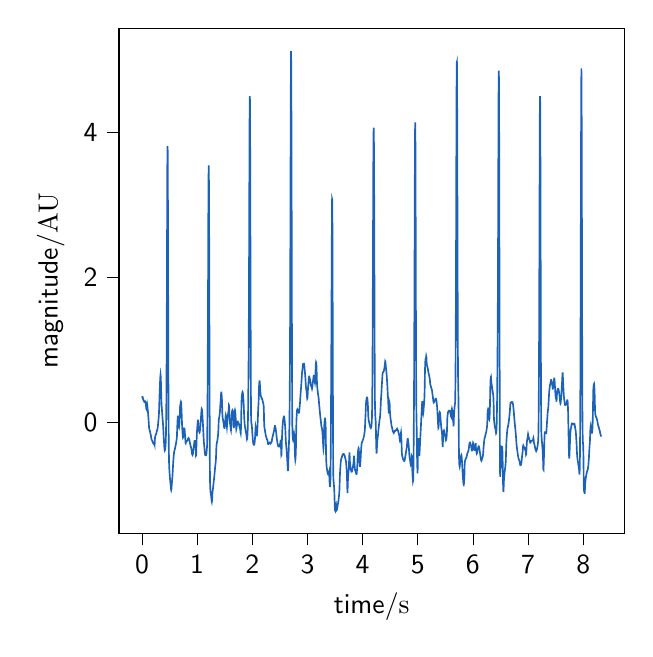
\begin{tikzpicture}
\pgfplotsset{
   every axis/.append style={
		font=\fontsize{10}{10}\sffamily},
	every non boxed x axis/.append style={
		x axis line style={->}
	},
	every non boxed y axis/.append style={
		y axis line style={->}
	},
	every non boxed z axis/.append style={
		z axis line style={->}
	}
}
\begin{axis}[
height=\figH,
tick align=outside,
tick pos=left,
width=\figW,
x grid style={white!69.0196078431373!black},
xlabel={time/$\si{\second}$},
xmin=-0.416499996185303, xmax=8.74649991989136,
xtick style={color=black},
y grid style={white!69.0196078431373!black},
ylabel={magnitude/\si{AU}},
ymin=-1.54407114386559, ymax=5.44581086039543,
ytick style={color=black},
ytick = {0, 2, 4},
yticklabels = {0, 2, 4},
xtick = {0, 1, 2, 3, 4, 5, 6, 7, 8},
xticklabels = {0, 1, 2, 3, 4, 5, 6, 7, 8},
]
\addplot [semithick, tud1b]
table {%
0 0.354356855154037
0.00333333341404796 0.349087834358215
0.00666666682809591 0.343818813562393
0.00999999977648258 0.343818813562393
0.0133333336561918 0.343818813562393
0.0166666675359011 0.333280742168427
0.0199999995529652 0.31747367978096
0.0233333334326744 0.306935638189316
0.0266666673123837 0.301666617393494
0.0299999993294477 0.296397596597672
0.0333333350718021 0.296397596597672
0.0366666652262211 0.285859555006027
0.0399999991059303 0.280590534210205
0.0433333329856396 0.275321513414383
0.0466666668653488 0.275321513414383
0.0500000007450581 0.280590534210205
0.0533333346247673 0.285859555006027
0.0566666685044765 0.285859555006027
0.0599999986588955 0.280590534210205
0.0633333325386047 0.264783471822739
0.0666666701436043 0.254245430231094
0.0700000002980232 0.243707403540611
0.0733333304524422 0.227900341153145
0.0766666680574417 0.185748174786568
0.0799999982118607 0.180479153990746
0.0833333358168602 0.201555237174034
0.0866666659712791 0.212093278765678
0.0900000035762787 0.233169361948967
0.0933333337306976 0.248976424336433
0.0966666638851166 0.233169361948967
0.100000001490116 0.201555237174034
0.103333331644535 0.175210133194923
0.106666669249535 0.154134064912796
0.109999999403954 0.127788960933685
0.113333337008953 0.0961748361587524
0.116666667163372 0.059291698038578
0.119999997317791 0.0224085561931133
0.123333334922791 -0.0144745847210288
0.126666665077209 -0.0566267482936382
0.129999995231628 -0.0882408767938614
0.133333340287209 -0.0987789109349251
0.136666670441628 -0.109316952526569
0.140000000596046 -0.114585973322392
0.143333330750465 -0.125124022364616
0.146666660904884 -0.135662049055099
0.150000005960464 -0.151469111442566
0.153333336114883 -0.16200715303421
0.156666666269302 -0.172545194625854
0.159999996423721 -0.177814215421677
0.16333332657814 -0.193621277809143
0.16666667163372 -0.214697360992432
0.170000001788139 -0.230504423379898
0.173333331942558 -0.241042464971542
0.176666662096977 -0.246311485767365
0.180000007152557 -0.251580506563187
0.183333337306976 -0.256849527359009
0.186666667461395 -0.262118548154831
0.189999997615814 -0.267387568950653
0.193333327770233 -0.277925610542297
0.196666672825813 -0.28319463133812
0.200000002980232 -0.288463652133942
0.203333333134651 -0.293732672929764
0.20666666328907 -0.299001693725586
0.209999993443489 -0.304270714521408
0.213333338499069 -0.30953973531723
0.216666668653488 -0.30953973531723
0.219999998807907 -0.304270714521408
0.223333328962326 -0.299001693725586
0.226666674017906 -0.299001693725586
0.230000004172325 -0.30953973531723
0.233333334326744 -0.251580506563187
0.236666664481163 -0.219966381788254
0.239999994635582 -0.204159319400787
0.243333339691162 -0.193621277809143
0.246666669845581 -0.183083236217499
0.25 -0.172545194625854
0.253333330154419 -0.172545194625854
0.256666660308838 -0.167276173830032
0.259999990463257 -0.16200715303421
0.263333320617676 -0.151469111442566
0.266666680574417 -0.135662049055099
0.270000010728836 -0.125124022364616
0.273333340883255 -0.114585973322392
0.276666671037674 -0.104047931730747
0.280000001192093 -0.0987789109349251
0.283333331346512 -0.0882408767938614
0.286666661500931 -0.0724338069558144
0.28999999165535 -0.0460887067019939
0.293333321809769 -0.0197436045855284
0.296666651964188 0.0118705164641142
0.300000011920929 0.0382156185805798
0.303333342075348 0.0645607188344002
0.306666672229767 0.101443856954575
0.310000002384186 0.159403070807457
0.313333332538605 0.243707403540611
0.316666662693024 0.322742700576782
0.319999992847443 0.396509021520615
0.323333323001862 0.46500626206398
0.326666653156281 0.533503532409668
0.330000013113022 0.586193740367889
0.333333343267441 0.633614897727966
0.33666667342186 0.654690980911255
0.340000003576279 0.628345906734467
0.343333333730698 0.565117657184601
0.346666663885117 0.470275282859802
0.349999994039536 0.338549792766571
0.353333324193954 0.259514451026917
0.356666654348373 0.222631320357323
0.360000014305115 0.19101719558239
0.363333344459534 0.154134064912796
0.366666674613953 0.117250919342041
0.370000004768372 0.0803677812218666
0.373333334922791 0.0434846356511116
0.376666665077209 0.0118705164641142
0.379999995231628 -0.0144745847210288
0.383333325386047 -0.0513577274978161
0.386666655540466 -0.0935098901391029
0.389999985694885 -0.151469111442566
0.393333345651627 -0.204159319400787
0.396666675806046 -0.241042464971542
0.400000005960464 -0.28319463133812
0.403333336114883 -0.325346797704697
0.406666666269302 -0.362229913473129
0.409999996423721 -0.383305996656418
0.41333332657814 -0.393844038248062
0.416666656732559 -0.38857501745224
0.419999986886978 -0.378036975860596
0.423333346843719 -0.356960892677307
0.426666676998138 -0.330615818500519
0.430000007152557 -0.293732672929764
0.433333337306976 -0.225235402584076
0.436666667461395 -0.0935098901391029
0.439999997615814 0.0961748361587524
0.443333327770233 0.407047063112259
0.446666657924652 0.87072080373764
0.449999988079071 1.49246525764465
0.453333348035812 2.23012804985046
0.456666678190231 2.98886680603027
0.46000000834465 3.6053421497345
0.463333338499069 3.81610298156738
0.466666668653488 3.74760580062866
0.469999998807907 3.19962763786316
0.473333328962326 2.26174211502075
0.476666659116745 1.23955225944519
0.479999989271164 0.407047063112259
0.483333319425583 -0.109316952526569
0.486666679382324 -0.367498934268951
0.490000009536743 -0.525569558143616
0.493333339691162 -0.62041187286377
0.496666669845581 -0.662564039230347
0.5 -0.699447214603424
0.503333330154419 -0.736330389976501
0.506666660308838 -0.773213505744934
0.509999990463257 -0.799558639526367
0.513333320617676 -0.825903713703156
0.516666650772095 -0.846979796886444
0.519999980926514 -0.878593921661377
0.523333311080933 -0.91020804643631
0.526666641235352 -0.931284129619598
0.529999971389771 -0.941822171211243
0.533333361148834 -0.931284129619598
0.536666691303253 -0.90493905544281
0.540000021457672 -0.868055880069733
0.543333351612091 -0.8364417552948
0.54666668176651 -0.804827630519867
0.550000011920929 -0.773213505744934
0.553333342075348 -0.736330389976501
0.556666672229767 -0.694178223609924
0.560000002384186 -0.646757006645203
0.563333332538605 -0.599335789680481
0.566666662693024 -0.557183682918549
0.569999992847443 -0.520300507545471
0.573333323001862 -0.488686382770538
0.576666653156281 -0.457072257995605
0.579999983310699 -0.435996174812317
0.583333313465118 -0.414920121431351
0.586666643619537 -0.404382079839706
0.589999973773956 -0.393844038248062
0.593333303928375 -0.383305996656418
0.596666693687439 -0.372767955064774
0.600000023841858 -0.362229913473129
0.603333353996277 -0.346422851085663
0.606666684150696 -0.335884839296341
0.610000014305115 -0.325346797704697
0.613333344459534 -0.314808756113052
0.616666674613953 -0.299001693725586
0.620000004768372 -0.28319463133812
0.623333334922791 -0.267387568950653
0.626666665077209 -0.251580506563187
0.629999995231628 -0.23577344417572
0.633333325386047 -0.204159319400787
0.636666655540466 -0.130393028259277
0.639999985694885 -0.0618957690894604
0.643333315849304 -0.00393654452636838
0.646666646003723 0.0434846356511116
0.649999976158142 0.0750987604260445
0.653333306312561 0.0750987604260445
0.656666696071625 0.0487536564469337
0.660000026226044 0.0224085561931133
0.663333356380463 -0.00393654452636838
0.666666686534882 -0.0302816461771727
0.670000016689301 -0.0566267482936382
0.673333346843719 -0.0671647861599922
0.676666676998138 -0.0513577274978161
0.680000007152557 -0.00393654452636838
0.683333337306976 0.0540226772427559
0.686666667461395 0.117250919342041
0.689999997615814 0.201555237174034
0.693333327770233 0.233169361948967
0.696666657924652 0.243707403540611
0.699999988079071 0.254245430231094
0.70333331823349 0.270052492618561
0.706666648387909 0.280590534210205
0.709999978542328 0.275321513414383
0.713333308696747 0.227900341153145
0.716666638851166 0.164672091603279
0.720000028610229 0.106712877750397
0.723333358764648 0.0276775769889355
0.726666688919067 -0.0355506651103497
0.730000019073486 -0.0829718485474586
0.733333349227905 -0.125124022364616
0.736666679382324 -0.167276173830032
0.740000009536743 -0.198890298604965
0.743333339691162 -0.214697360992432
0.746666669845581 -0.209428340196609
0.75 -0.193621277809143
0.753333330154419 -0.172545194625854
0.756666660308838 -0.156738132238388
0.759999990463257 -0.135662049055099
0.763333320617676 -0.109316952526569
0.766666650772095 -0.0882408767938614
0.769999980926514 -0.0882408767938614
0.773333311080933 -0.109316952526569
0.776666641235352 -0.140931069850922
0.779999971389771 -0.177814215421677
0.783333361148834 -0.209428340196609
0.786666691303253 -0.251580506563187
0.790000021457672 -0.288463652133942
0.793333351612091 -0.293732672929764
0.79666668176651 -0.28319463133812
0.800000011920929 -0.277925610542297
0.803333342075348 -0.272656589746475
0.806666672229767 -0.272656589746475
0.810000002384186 -0.267387568950653
0.813333332538605 -0.262118548154831
0.816666662693024 -0.262118548154831
0.819999992847443 -0.256849527359009
0.823333323001862 -0.256849527359009
0.826666653156281 -0.251580506563187
0.829999983310699 -0.246311485767365
0.833333313465118 -0.23577344417572
0.836666643619537 -0.23577344417572
0.839999973773956 -0.230504423379898
0.843333303928375 -0.23577344417572
0.846666693687439 -0.23577344417572
0.850000023841858 -0.230504423379898
0.853333353996277 -0.23577344417572
0.856666684150696 -0.241042464971542
0.860000014305115 -0.251580506563187
0.863333344459534 -0.267387568950653
0.866666674613953 -0.277925610542297
0.870000004768372 -0.293732672929764
0.873333334922791 -0.304270714521408
0.876666665077209 -0.314808756113052
0.879999995231628 -0.325346797704697
0.883333325386047 -0.335884839296341
0.886666655540466 -0.341153830289841
0.889999985694885 -0.351691871881485
0.893333315849304 -0.362229913473129
0.896666646003723 -0.372767955064774
0.899999976158142 -0.393844038248062
0.903333306312561 -0.409651100635529
0.906666696071625 -0.430727183818817
0.910000026226044 -0.446534216403961
0.913333356380463 -0.451803237199783
0.916666686534882 -0.457072257995605
0.920000016689301 -0.451803237199783
0.923333346843719 -0.441265195608139
0.926666676998138 -0.425458163022995
0.930000007152557 -0.404382079839706
0.933333337306976 -0.383305996656418
0.936666667461395 -0.362229913473129
0.939999997615814 -0.341153830289841
0.943333327770233 -0.320077776908875
0.946666657924652 -0.293732672929764
0.949999988079071 -0.277925610542297
0.95333331823349 -0.262118548154831
0.956666648387909 -0.262118548154831
0.959999978542328 -0.262118548154831
0.963333308696747 -0.277925610542297
0.966666638851166 -0.299001693725586
0.970000028610229 -0.325346797704697
0.973333358764648 -0.351691871881485
0.976666688919067 -0.393844038248062
0.980000019073486 -0.462341278791428
0.983333349227905 -0.457072257995605
0.986666679382324 -0.356960892677307
0.990000009536743 -0.272656589746475
0.993333339691162 -0.198890298604965
0.996666669845581 -0.140931069850922
1 -0.0987789109349251
1.00333333015442 -0.0724338069558144
1.00666666030884 -0.0408196859061718
1.00999999046326 -0.00393654452636838
1.01333332061768 0.0224085561931133
1.01666665077209 0.0224085561931133
1.01999998092651 -0.0144745847210288
1.02333331108093 -0.0566267482936382
1.02666664123535 -0.0777028277516365
1.02999997138977 -0.0935098901391029
1.03333330154419 -0.114585973322392
1.03666663169861 -0.130393028259277
1.03999996185303 -0.140931069850922
1.04333329200745 -0.146200090646744
1.04666662216187 -0.140931069850922
1.04999995231628 -0.125124022364616
1.0533332824707 -0.0987789109349251
1.05666661262512 -0.0724338069558144
1.05999994277954 -0.0408196859061718
1.06333339214325 -0.00393654452636838
1.06666672229767 0.0276775769889355
1.07000005245209 0.0645607188344002
1.07333338260651 0.101443856954575
1.07666671276093 0.13832700252533
1.08000004291534 0.164672091603279
1.08333337306976 0.180479153990746
1.08666670322418 0.175210133194923
1.0900000333786 0.154134064912796
1.09333336353302 0.122519932687283
1.09666669368744 0.0803677812218666
1.10000002384186 0.0382156185805798
1.10333335399628 -0.00393654452636838
1.1066666841507 -0.0513577274978161
1.11000001430511 -0.0987789109349251
1.11333334445953 -0.151469111442566
1.11666667461395 -0.204159319400787
1.12000000476837 -0.251580506563187
1.12333333492279 -0.288463652133942
1.12666666507721 -0.314808756113052
1.12999999523163 -0.341153830289841
1.13333332538605 -0.372767955064774
1.13666665554047 -0.404382079839706
1.13999998569489 -0.430727183818817
1.1433333158493 -0.446534216403961
1.14666664600372 -0.457072257995605
1.14999997615814 -0.462341278791428
1.15333330631256 -0.462341278791428
1.15666663646698 -0.462341278791428
1.1599999666214 -0.462341278791428
1.16333329677582 -0.462341278791428
1.16666662693024 -0.451803237199783
1.16999995708466 -0.430727183818817
1.17333328723907 -0.399113059043884
1.17666661739349 -0.367498934268951
1.17999994754791 -0.341153830289841
1.18333327770233 -0.198890298604965
1.18666660785675 0.0698297396302223
1.19000005722046 0.449199199676514
1.19333338737488 0.94975608587265
1.1966667175293 1.57150053977966
1.20000004768372 2.27228021621704
1.20333337783813 2.93617653846741
1.20666670799255 3.38931226730347
1.21000003814697 3.54738306999207
1.21333336830139 3.4051194190979
1.21666669845581 2.96252179145813
1.22000002861023 2.14582371711731
1.22333335876465 1.19740009307861
1.22666668891907 0.248976424336433
1.23000001907349 -0.509762465953827
1.23333334922791 -0.804827630519867
1.23666667938232 -0.894401013851166
1.24000000953674 -0.941822171211243
1.24333333969116 -0.968167245388031
1.24666666984558 -0.98924332857132
1.25 -1.00505042076111
1.25333333015442 -1.02085745334625
1.25666666030884 -1.04193353652954
1.25999999046326 -1.06827867031097
1.26333332061768 -1.09462380409241
1.26666665077209 -1.10516178607941
1.26999998092651 -1.08935475349426
1.27333331108093 -1.04720258712769
1.27666664123535 -0.994512379169464
1.27999997138977 -0.962898254394531
1.28333330154419 -0.941822171211243
1.28666663169861 -0.920746088027954
1.28999996185303 -0.90493905544281
1.29333329200745 -0.878593921661377
1.29666662216187 -0.857517838478088
1.29999995231628 -0.8311727643013
1.3033332824707 -0.810096681118011
1.30666661262512 -0.783751547336578
1.30999994277954 -0.76267546415329
1.31333339214325 -0.736330389976501
1.31666672229767 -0.709985256195068
1.32000005245209 -0.678371131420135
1.32333338260651 -0.652025997638702
1.32666671276093 -0.62041187286377
1.33000004291534 -0.599335789680481
1.33333337306976 -0.578259706497192
1.33666670322418 -0.551914632320404
1.3400000333786 -0.525569558143616
1.34333336353302 -0.46761029958725
1.34666669368744 -0.38857501745224
1.35000002384186 -0.335884839296341
1.35333335399628 -0.30953973531723
1.3566666841507 -0.293732672929764
1.36000001430511 -0.28319463133812
1.36333334445953 -0.272656589746475
1.36666667461395 -0.256849527359009
1.37000000476837 -0.241042464971542
1.37333333492279 -0.219966381788254
1.37666666507721 -0.198890298604965
1.37999999523163 -0.172545194625854
1.38333332538605 -0.135662049055099
1.38666665554047 -0.0882408767938614
1.38999998569489 -0.0144745847210288
1.3933333158493 0.0329465977847576
1.39666664600372 0.0487536564469337
1.39999997615814 0.0645607188344002
1.40333330631256 0.0750987604260445
1.40666663646698 0.0961748361587524
1.4099999666214 0.117250919342041
1.41333329677582 0.143596023321152
1.41666662693024 0.180479153990746
1.41999995708466 0.222631320357323
1.42333328723907 0.259514451026917
1.42666661739349 0.291128575801849
1.42999994754791 0.333280742168427
1.43333327770233 0.380701959133148
1.43666660785675 0.407047063112259
1.44000005722046 0.407047063112259
1.44333338737488 0.38597097992897
1.4466667175293 0.349087834358215
1.45000004768372 0.306935638189316
1.45333337783813 0.222631320357323
1.45666670799255 0.117250919342041
1.46000003814697 0.0803677812218666
1.46333336830139 0.059291698038578
1.46666669845581 0.0434846356511116
1.47000002861023 0.0276775769889355
1.47333335876465 0.0118705164641142
1.47666668891907 -0.00393654452636838
1.48000001907349 -0.0197436045855284
1.48333334922791 -0.0355506651103497
1.48666667938232 -0.0566267482936382
1.49000000953674 -0.0777028277516365
1.49333333969116 -0.0829718485474586
1.49666666984558 -0.0829718485474586
1.5 -0.0671647861599922
1.50333333015442 -0.0408196859061718
1.50666666030884 -0.00920556485652924
1.50999999046326 0.0118705164641142
1.51333332061768 0.0487536564469337
1.51666665077209 0.0803677812218666
1.51999998092651 0.0961748361587524
1.52333331108093 0.0856367945671082
1.52666664123535 0.059291698038578
1.52999997138977 0.0276775769889355
1.53333330154419 -0.00393654452636838
1.53666663169861 -0.0513577274978161
1.53999996185303 -0.0724338069558144
1.54333329200745 -0.0460887067019939
1.54666662216187 0.00133247557096183
1.54999995231628 0.0329465977847576
1.5533332824707 0.059291698038578
1.55666661262512 0.0856367945671082
1.55999994277954 0.106712877750397
1.56333339214325 0.122519932687283
1.56666672229767 0.13832700252533
1.57000005245209 0.159403070807457
1.57333338260651 0.185748174786568
1.57666671276093 0.233169361948967
1.58000004291534 0.227900341153145
1.58333337306976 0.154134064912796
1.58666670322418 0.0961748361587524
1.5900000333786 0.0487536564469337
1.59333336353302 0.00660149566829205
1.59666669368744 -0.0197436045855284
1.60000002384186 -0.0408196859061718
1.60333335399628 -0.0566267482936382
1.6066666841507 -0.0777028277516365
1.61000001430511 -0.104047931730747
1.61333334445953 -0.114585973322392
1.61666667461395 -0.0777028277516365
1.62000000476837 -0.00393654452636838
1.62333333492279 0.0382156185805798
1.62666666507721 0.0750987604260445
1.62999999523163 0.111981898546219
1.63333332538605 0.143596023321152
1.63666665554047 0.159403070807457
1.63999998569489 0.164672091603279
1.6433333158493 0.159403070807457
1.64666664600372 0.143596023321152
1.64999997615814 0.122519932687283
1.65333330631256 0.0909058153629303
1.65666663646698 0.0276775769889355
1.6599999666214 -0.0408196859061718
1.66333329677582 -0.0671647861599922
1.66666662693024 -0.0829718485474586
1.66999995708466 -0.00920556485652924
1.67333328723907 0.0540226772427559
1.67666661739349 0.0909058153629303
1.67999994754791 0.127788960933685
1.68333327770233 0.154134064912796
1.68666660785675 0.164672091603279
1.69000005722046 0.154134064912796
1.69333338737488 0.122519932687283
1.6966667175293 0.0856367945671082
1.70000004768372 0.0434846356511116
1.70333337783813 0.00133247557096183
1.70666670799255 -0.0671647861599922
1.71000003814697 -0.0987789109349251
1.71333336830139 -0.0882408767938614
1.71666669845581 -0.0671647861599922
1.72000002861023 -0.0513577274978161
1.72333335876465 -0.0355506651103497
1.72666668891907 -0.0144745847210288
1.73000001907349 0.00133247557096183
1.73333334922791 0.00660149566829205
1.73666667938232 0.00660149566829205
1.74000000953674 0.00133247557096183
1.74333333969116 -0.00393654452636838
1.74666666984558 -0.00920556485652924
1.75 -0.0144745847210288
1.75333333015442 -0.0197436045855284
1.75666666030884 -0.0250126253813505
1.75999999046326 -0.0355506651103497
1.76333332061768 -0.0513577274978161
1.76666665077209 -0.0618957690894604
1.76999998092651 -0.0724338069558144
1.77333331108093 -0.0777028277516365
1.77666664123535 -0.0882408767938614
1.77999997138977 -0.0987789109349251
1.78333330154419 -0.119854994118214
1.78666663169861 -0.146200090646744
1.78999996185303 -0.156738132238388
1.79333329200745 -0.119854994118214
1.79666662216187 -0.0355506651103497
1.79999995231628 0.0909058153629303
1.8033332824707 0.254245430231094
1.80666661262512 0.31747367978096
1.80999994277954 0.354356855154037
1.81333339214325 0.375432938337326
1.81666672229767 0.396509021520615
1.82000005245209 0.412316083908081
1.82333338260651 0.417585074901581
1.82666671276093 0.412316083908081
1.83000004291534 0.396509021520615
1.83333337306976 0.370163917541504
1.83666670322418 0.338549792766571
1.8400000333786 0.301666617393494
1.84333336353302 0.259514451026917
1.84666669368744 0.196286216378212
1.85000002384186 0.133057981729507
1.85333335399628 0.0698297396302223
1.8566666841507 0.0224085561931133
1.86000001430511 -0.00920556485652924
1.86333334445953 -0.0408196859061718
1.86666667461395 -0.0618957690894604
1.87000000476837 -0.0777028277516365
1.87333333492279 -0.0935098901391029
1.87666666507721 -0.109316952526569
1.87999999523163 -0.125124022364616
1.88333332538605 -0.135662049055099
1.88666665554047 -0.151469111442566
1.88999998569489 -0.16200715303421
1.8933333158493 -0.177814215421677
1.89666664600372 -0.204159319400787
1.89999997615814 -0.225235402584076
1.90333330631256 -0.241042464971542
1.90666663646698 -0.23577344417572
1.9099999666214 -0.214697360992432
1.91333329677582 -0.172545194625854
1.91666662693024 -0.114585973322392
1.91999995708466 -0.0197436045855284
1.92333328723907 0.122519932687283
1.92666661739349 0.338549792766571
1.92999994754791 0.580924689769745
1.93333327770233 0.886527836322784
1.93666660785675 1.30804944038391
1.94000005722046 1.88237273693085
1.94333338737488 2.59895944595337
1.9466667175293 3.37350535392761
1.95000004768372 4.07955408096313
1.95333337783813 4.48526859283447
1.95666670799255 4.50634479522705
1.96000003814697 4.18493461608887
1.96333336830139 3.4051194190979
1.96666669845581 2.41981291770935
1.97000002861023 1.43977510929108
1.97333335876465 0.638883948326111
1.97666668891907 0.13832700252533
1.98000001907349 0.0171395353972912
1.98333334922791 -0.00920556485652924
1.98666667938232 -0.0250126253813505
1.99000000953674 -0.0408196859061718
1.99333333969116 -0.0724338069558144
1.99666666984558 -0.104047931730747
2 -0.146200090646744
2.00333333015442 -0.183083236217499
2.00666666030884 -0.214697360992432
2.00999999046326 -0.246311485767365
2.01333332061768 -0.272656589746475
2.01666665077209 -0.293732672929764
2.01999998092651 -0.304270714521408
2.02333331108093 -0.30953973531723
2.02666664123535 -0.314808756113052
2.02999997138977 -0.314808756113052
2.03333330154419 -0.314808756113052
2.03666663169861 -0.30953973531723
2.03999996185303 -0.299001693725586
2.04333329200745 -0.277925610542297
2.04666662216187 -0.251580506563187
2.04999995231628 -0.214697360992432
2.0533332824707 -0.177814215421677
2.05666661262512 -0.104047931730747
2.05999994277954 -0.0724338069558144
2.06333327293396 -0.0882408767938614
2.06666660308838 -0.125124022364616
2.0699999332428 -0.146200090646744
2.07333326339722 -0.16200715303421
2.07666659355164 -0.177814215421677
2.07999992370605 -0.188352257013321
2.08333325386047 -0.188352257013321
2.08666658401489 -0.167276173830032
2.08999991416931 -0.125124022364616
2.09333324432373 -0.0777028277516365
2.09666657447815 -0.0302816461771727
2.09999990463257 0.0276775769889355
2.10333323478699 0.101443856954575
2.10666656494141 0.175210133194923
2.10999989509583 0.217362299561501
2.11333322525024 0.254245430231094
2.11666655540466 0.328011721372604
2.11999988555908 0.433392137289047
2.1233332157135 0.501889407634735
2.1266667842865 0.538772583007812
2.13000011444092 0.565117657184601
2.13333344459534 0.565117657184601
2.13666677474976 0.538772583007812
2.14000010490417 0.496620386838913
2.14333343505859 0.459737241268158
2.14666676521301 0.417585074901581
2.15000009536743 0.391240000724792
2.15333342552185 0.370163917541504
2.15666675567627 0.354356855154037
2.16000008583069 0.349087834358215
2.16333341598511 0.343818813562393
2.16666674613953 0.338549792766571
2.17000007629395 0.328011721372604
2.17333340644836 0.322742700576782
2.17666673660278 0.31747367978096
2.1800000667572 0.31747367978096
2.18333339691162 0.306935638189316
2.18666672706604 0.296397596597672
2.19000005722046 0.285859555006027
2.19333338737488 0.275321513414383
2.1966667175293 0.264783471822739
2.20000004768372 0.254245430231094
2.20333337783813 0.238438382744789
2.20666670799255 0.217362299561501
2.21000003814697 0.164672091603279
2.21333336830139 0.0224085561931133
2.21666669845581 -0.0513577274978161
2.22000002861023 -0.0777028277516365
2.22333335876465 -0.0882408767938614
2.22666668891907 -0.104047931730747
2.23000001907349 -0.119854994118214
2.23333334922791 -0.135662049055099
2.23666667938232 -0.151469111442566
2.24000000953674 -0.167276173830032
2.24333333969116 -0.183083236217499
2.24666666984558 -0.193621277809143
2.25 -0.198890298604965
2.25333333015442 -0.209428340196609
2.25666666030884 -0.219966381788254
2.25999999046326 -0.230504423379898
2.26333332061768 -0.23577344417572
2.26666665077209 -0.241042464971542
2.26999998092651 -0.241042464971542
2.27333331108093 -0.246311485767365
2.27666664123535 -0.262118548154831
2.27999997138977 -0.277925610542297
2.28333330154419 -0.293732672929764
2.28666663169861 -0.304270714521408
2.28999996185303 -0.304270714521408
2.29333329200745 -0.299001693725586
2.29666662216187 -0.299001693725586
2.29999995231628 -0.299001693725586
2.3033332824707 -0.299001693725586
2.30666661262512 -0.299001693725586
2.30999994277954 -0.293732672929764
2.31333327293396 -0.288463652133942
2.31666660308838 -0.28319463133812
2.3199999332428 -0.28319463133812
2.32333326339722 -0.288463652133942
2.32666659355164 -0.288463652133942
2.32999992370605 -0.293732672929764
2.33333325386047 -0.288463652133942
2.33666658401489 -0.288463652133942
2.33999991416931 -0.288463652133942
2.34333324432373 -0.288463652133942
2.34666657447815 -0.28319463133812
2.34999990463257 -0.277925610542297
2.35333323478699 -0.267387568950653
2.35666656494141 -0.251580506563187
2.35999989509583 -0.230504423379898
2.36333322525024 -0.219966381788254
2.36666655540466 -0.209428340196609
2.36999988555908 -0.198890298604965
2.3733332157135 -0.188352257013321
2.3766667842865 -0.177814215421677
2.38000011444092 -0.167276173830032
2.38333344459534 -0.156738132238388
2.38666677474976 -0.146200090646744
2.39000010490417 -0.135662049055099
2.39333343505859 -0.125124022364616
2.39666676521301 -0.109316952526569
2.40000009536743 -0.0882408767938614
2.40333342552185 -0.0777028277516365
2.40666675567627 -0.0671647861599922
2.41000008583069 -0.0566267482936382
2.41333341598511 -0.0566267482936382
2.41666674613953 -0.0671647861599922
2.42000007629395 -0.0777028277516365
2.42333340644836 -0.0882408767938614
2.42666673660278 -0.104047931730747
2.4300000667572 -0.125124022364616
2.43333339691162 -0.151469111442566
2.43666672706604 -0.172545194625854
2.44000005722046 -0.198890298604965
2.44333338737488 -0.219966381788254
2.4466667175293 -0.241042464971542
2.45000004768372 -0.256849527359009
2.45333337783813 -0.272656589746475
2.45666670799255 -0.293732672929764
2.46000003814697 -0.304270714521408
2.46333336830139 -0.314808756113052
2.46666669845581 -0.325346797704697
2.47000002861023 -0.335884839296341
2.47333335876465 -0.341153830289841
2.47666668891907 -0.341153830289841
2.48000001907349 -0.341153830289841
2.48333334922791 -0.341153830289841
2.48666667938232 -0.341153830289841
2.49000000953674 -0.330615818500519
2.49333333969116 -0.325346797704697
2.49666666984558 -0.320077776908875
2.5 -0.314808756113052
2.50333333015442 -0.304270714521408
2.50666666030884 -0.299001693725586
2.50999999046326 -0.28319463133812
2.51333332061768 -0.256849527359009
2.51666665077209 -0.256849527359009
2.51999998092651 -0.325346797704697
2.52333331108093 -0.393844038248062
2.52666664123535 -0.462341278791428
2.52999997138977 -0.457072257995605
2.53333330154419 -0.356960892677307
2.53666663169861 -0.267387568950653
2.53999996185303 -0.193621277809143
2.54333329200745 -0.130393028259277
2.54666662216187 -0.0829718485474586
2.54999995231628 -0.0460887067019939
2.5533332824707 -0.0197436045855284
2.55666661262512 0.00660149566829205
2.55999994277954 0.0276775769889355
2.56333327293396 0.0487536564469337
2.56666660308838 0.059291698038578
2.5699999332428 0.0698297396302223
2.57333326339722 0.0750987604260445
2.57666659355164 0.0750987604260445
2.57999992370605 0.0645607188344002
2.58333325386047 0.0487536564469337
2.58666658401489 0.0224085561931133
2.58999991416931 -0.00920556485652924
2.59333324432373 -0.0408196859061718
2.59666657447815 -0.0777028277516365
2.59999990463257 -0.114585973322392
2.60333323478699 -0.177814215421677
2.60666656494141 -0.241042464971542
2.60999989509583 -0.28319463133812
2.61333322525024 -0.314808756113052
2.61666655540466 -0.346422851085663
2.61999988555908 -0.372767955064774
2.6233332157135 -0.409651100635529
2.6266667842865 -0.446534216403961
2.63000011444092 -0.483417361974716
2.63333344459534 -0.520300507545471
2.63666677474976 -0.562452673912048
2.64000010490417 -0.604604840278625
2.64333343505859 -0.657295048236847
2.64666676521301 -0.678371131420135
2.65000009536743 -0.641487956047058
2.65333342552185 -0.557183682918549
2.65666675567627 -0.483417361974716
2.66000008583069 -0.399113059043884
2.66333341598511 -0.325346797704697
2.66666674613953 -0.267387568950653
2.67000007629395 -0.167276173830032
2.67333340644836 -0.0355506651103497
2.67666673660278 0.196286216378212
2.6800000667572 0.486082345247269
2.68333339691162 0.939218044281006
2.68666672706604 1.60311472415924
2.69000005722046 2.46196508407593
2.69333338737488 3.42092657089233
2.6966667175293 4.29558372497559
2.70000004768372 4.9015212059021
2.70333337783813 5.12808895111084
2.70666670799255 4.89098310470581
2.71000003814697 4.19547271728516
2.71333336830139 3.16274452209473
2.71666669845581 1.97721517086029
2.72000002861023 0.886527836322784
2.72333335876465 0.101443856954575
2.72666668891907 -0.109316952526569
2.73000001907349 -0.167276173830032
2.73333334922791 -0.209428340196609
2.73666667938232 -0.241042464971542
2.74000000953674 -0.251580506563187
2.74333333969116 -0.246311485767365
2.74666666984558 -0.241042464971542
2.75 -0.230504423379898
2.75333333015442 -0.219966381788254
2.75666666030884 -0.204159319400787
2.75999999046326 -0.172545194625854
2.76333332061768 -0.188352257013321
2.76666665077209 -0.293732672929764
2.76999998092651 -0.367498934268951
2.77333331108093 -0.441265195608139
2.77666664123535 -0.499224424362183
2.77999997138977 -0.525569558143616
2.78333330154419 -0.509762465953827
2.78666663169861 -0.462341278791428
2.78999996185303 -0.393844038248062
2.79333329200745 -0.299001693725586
2.79666662216187 -0.109316952526569
2.79999995231628 0.00660149566829205
2.8033332824707 0.0645607188344002
2.80666661262512 0.111981898546219
2.80999994277954 0.154134064912796
2.81333327293396 0.169941112399101
2.81666660308838 0.175210133194923
2.8199999332428 0.169941112399101
2.82333326339722 0.164672091603279
2.82666659355164 0.164672091603279
2.82999992370605 0.159403070807457
2.83333325386047 0.154134064912796
2.83666658401489 0.148865044116974
2.83999991416931 0.13832700252533
2.84333324432373 0.127788960933685
2.84666657447815 0.127788960933685
2.84999990463257 0.13832700252533
2.85333323478699 0.164672091603279
2.85666656494141 0.19101719558239
2.85999989509583 0.222631320357323
2.86333322525024 0.248976424336433
2.86666655540466 0.280590534210205
2.86999988555908 0.31747367978096
2.8733332157135 0.364894896745682
2.8766667842865 0.401778042316437
2.88000011444092 0.433392137289047
2.88333344459534 0.46500626206398
2.88666677474976 0.491351366043091
2.89000010490417 0.533503532409668
2.89333343505859 0.575655698776245
2.89666676521301 0.617807865142822
2.90000009536743 0.659960031509399
2.90333342552185 0.691574096679688
2.90666675567627 0.712650179862976
2.91000008583069 0.728457272052765
2.91333341598511 0.749533295631409
2.91666674613953 0.775878429412842
2.92000007629395 0.79695451259613
2.92333340644836 0.807492554187775
2.92666673660278 0.807492554187775
2.9300000667572 0.807492554187775
2.93333339691162 0.807492554187775
2.93666672706604 0.807492554187775
2.94000005722046 0.79695451259613
2.94333338737488 0.781147420406342
2.9466667175293 0.754802346229553
2.95000004768372 0.72318822145462
2.95333337783813 0.691574096679688
2.95666670799255 0.665229022502899
2.96000003814697 0.638883948326111
2.96333336830139 0.602000772953033
2.96666669845581 0.559848606586456
2.97000002861023 0.512427449226379
2.97333335876465 0.480813324451447
2.97666668891907 0.459737241268158
2.98000001907349 0.443930178880692
2.98333334922791 0.428123116493225
2.98666667938232 0.412316083908081
2.99000000953674 0.380701959133148
2.99333333969116 0.343818813562393
2.99666666984558 0.322742700576782
3 0.328011721372604
3.00333333015442 0.364894896745682
3.00666666030884 0.417585074901581
3.00999999046326 0.46500626206398
3.01333332061768 0.491351366043091
3.01666665077209 0.522965490818024
3.01999998092651 0.554579615592957
3.02333331108093 0.586193740367889
3.02666664123535 0.617807865142822
3.02999997138977 0.628345906734467
3.03333330154419 0.628345906734467
3.03666663169861 0.617807865142822
3.03999996185303 0.602000772953033
3.04333329200745 0.591462731361389
3.04666662216187 0.586193740367889
3.04999995231628 0.575655698776245
3.0533332824707 0.554579615592957
3.05666661262512 0.533503532409668
3.05999994277954 0.512427449226379
3.06333327293396 0.501889407634735
3.06666660308838 0.496620386838913
3.0699999332428 0.491351366043091
3.07333326339722 0.486082345247269
3.07666659355164 0.475544303655624
3.07999992370605 0.470275282859802
3.08333325386047 0.459737241268158
3.08666658401489 0.470275282859802
3.08999991416931 0.491351366043091
3.09333324432373 0.522965490818024
3.09666657447815 0.544041574001312
3.09999990463257 0.565117657184601
3.10333323478699 0.580924689769745
3.10666656494141 0.602000772953033
3.10999989509583 0.623076856136322
3.11333322525024 0.638883948326111
3.11666655540466 0.638883948326111
3.11999988555908 0.633614897727966
3.1233332157135 0.617807865142822
3.1266667842865 0.596731781959534
3.13000011444092 0.575655698776245
3.13333344459534 0.549310624599457
3.13666677474976 0.538772583007812
3.14000010490417 0.559848606586456
3.14333343505859 0.612538814544678
3.14666676521301 0.696843147277832
3.15000009536743 0.775878429412842
3.15333342552185 0.807492554187775
3.15666675567627 0.828568637371063
3.16000008583069 0.823299586772919
3.16333341598511 0.775878429412842
3.16666674613953 0.707381188869476
3.17000007629395 0.602000772953033
3.17333340644836 0.533503532409668
3.17666673660278 0.496620386838913
3.1800000667572 0.470275282859802
3.18333339691162 0.438661158084869
3.18666672706604 0.417585074901581
3.19000005722046 0.396509021520615
3.19333338737488 0.380701959133148
3.1966667175293 0.364894896745682
3.20000004768372 0.349087834358215
3.20333337783813 0.328011721372604
3.20666670799255 0.296397596597672
3.21000003814697 0.264783471822739
3.21333336830139 0.233169361948967
3.21666669845581 0.206824257969856
3.22000002861023 0.180479153990746
3.22333335876465 0.154134064912796
3.22666668891907 0.127788960933685
3.23000001907349 0.101443856954575
3.23333334922791 0.0750987604260445
3.23666667938232 0.0540226772427559
3.24000000953674 0.0329465977847576
3.24333333969116 0.0118705164641142
3.24666666984558 -0.0144745847210288
3.25 -0.0408196859061718
3.25333333015442 -0.0618957690894604
3.25666666030884 -0.0724338069558144
3.25999999046326 -0.0777028277516365
3.26333332061768 -0.0882408767938614
3.26666665077209 -0.104047931730747
3.26999998092651 -0.130393028259277
3.27333331108093 -0.16200715303421
3.27666664123535 -0.204159319400787
3.27999997138977 -0.251580506563187
3.28333330154419 -0.299001693725586
3.28666663169861 -0.341153830289841
3.28999996185303 -0.367498934268951
3.29333329200745 -0.346422851085663
3.29666662216187 -0.288463652133942
3.29999995231628 -0.204159319400787
3.3033332824707 -0.0829718485474586
3.30666661262512 -0.0302816461771727
3.30999994277954 0.00660149566829205
3.31333327293396 0.0329465977847576
3.31666660308838 0.0487536564469337
3.3199999332428 0.0487536564469337
3.32333326339722 0.0276775769889355
3.32666659355164 -0.00393654452636838
3.32999992370605 -0.0513577274978161
3.33333325386047 -0.209428340196609
3.33666658401489 -0.420189142227173
3.33999991416931 -0.520300507545471
3.34333324432373 -0.572990715503693
3.34666657447815 -0.609873831272125
3.34999990463257 -0.630949914455414
3.35333323478699 -0.652025997638702
3.35666656494141 -0.667833089828491
3.35999989509583 -0.678371131420135
3.36333322525024 -0.694178223609924
3.36666655540466 -0.709985256195068
3.36999988555908 -0.720523297786713
3.3733332157135 -0.725792348384857
3.3766667842865 -0.725792348384857
3.38000011444092 -0.720523297786713
3.38333344459534 -0.715254306793213
3.38666677474976 -0.709985256195068
3.39000010490417 -0.699447214603424
3.39333343505859 -0.68890917301178
3.39666676521301 -0.75740647315979
3.40000009536743 -0.815365672111511
3.40333342552185 -0.862786889076233
3.40666675567627 -0.889131963253021
3.41000008583069 -0.889131963253021
3.41333341598511 -0.857517838478088
3.41666674613953 -0.794289588928223
3.42000007629395 -0.61514288187027
3.42333340644836 -0.30953973531723
3.42666673660278 0.106712877750397
3.4300000667572 0.591462731361389
3.43333339691162 1.11309576034546
3.43666672706604 1.66634297370911
3.44000005722046 2.2459352016449
3.44333338737488 2.78337502479553
3.4466667175293 3.08370923995972
3.45000004768372 3.07317113876343
3.45333337783813 2.69380187988281
3.45666670799255 1.85602760314941
3.46000003814697 0.865451753139496
3.46333336830139 -0.0355506651103497
3.46666669845581 -0.636218965053558
3.47000002861023 -0.783751547336578
3.47333335876465 -0.815365672111511
3.47666668891907 -0.841710805892944
3.48000001907349 -0.873324930667877
3.48333334922791 -0.90493905544281
3.48666667938232 -0.947091221809387
3.49000000953674 -1.0261265039444
3.49333333969116 -1.1262378692627
3.49666666984558 -1.18419706821442
3.5 -1.22108030319214
3.50333333015442 -1.22634923458099
3.50666666030884 -1.20000422000885
3.50999999046326 -1.16839003562927
3.51333332061768 -1.13677597045898
3.51666665077209 -1.13150691986084
3.51999998092651 -1.15785205364227
3.52333331108093 -1.17892813682556
3.52666664123535 -1.19473516941071
3.52999997138977 -1.20527315139771
3.53333330154419 -1.21581125259399
3.53666663169861 -1.21054220199585
3.53999996185303 -1.19473516941071
3.54333329200745 -1.17365908622742
3.54666662216187 -1.15785205364227
3.54999995231628 -1.14204490184784
3.5533332824707 -1.13150691986084
3.55666661262512 -1.1156998872757
3.55999994277954 -1.09989273548126
3.56333327293396 -1.07881665229797
3.56666660308838 -1.05774056911469
3.5699999332428 -1.0366644859314
3.57333326339722 -1.01558840274811
3.57666659355164 -0.98397433757782
3.57999992370605 -0.941822171211243
3.58333325386047 -0.862786889076233
3.58666658401489 -0.778482556343079
3.58999991416931 -0.715254306793213
3.59333324432373 -0.673102080821991
3.59666657447815 -0.630949914455414
3.59999990463257 -0.594066798686981
3.60333323478699 -0.557183682918549
3.60666656494141 -0.53610759973526
3.60999989509583 -0.520300507545471
3.61333322525024 -0.509762465953827
3.61666655540466 -0.499224424362183
3.61999988555908 -0.49395540356636
3.6233332157135 -0.488686382770538
3.6266667842865 -0.478148341178894
3.63000011444092 -0.46761029958725
3.63333344459534 -0.462341278791428
3.63666677474976 -0.451803237199783
3.64000010490417 -0.451803237199783
3.64333343505859 -0.451803237199783
3.64666676521301 -0.446534216403961
3.65000009536743 -0.446534216403961
3.65333342552185 -0.441265195608139
3.65666675567627 -0.441265195608139
3.66000008583069 -0.446534216403961
3.66333341598511 -0.451803237199783
3.66666674613953 -0.457072257995605
3.67000007629395 -0.462341278791428
3.67333340644836 -0.462341278791428
3.67666673660278 -0.472879320383072
3.6800000667572 -0.483417361974716
3.68333339691162 -0.49395540356636
3.68666672706604 -0.504493474960327
3.69000005722046 -0.515031516551971
3.69333338737488 -0.525569558143616
3.6966667175293 -0.53610759973526
3.70000004768372 -0.557183682918549
3.70333337783813 -0.583528757095337
3.70666670799255 -0.61514288187027
3.71000003814697 -0.646757006645203
3.71333336830139 -0.68890917301178
3.71666669845581 -0.75740647315979
3.72000002861023 -0.857517838478088
3.72333335876465 -0.931284129619598
3.72666668891907 -0.98397433757782
3.73000001907349 -0.894401013851166
3.73333334922791 -0.820634722709656
3.73666667938232 -0.773213505744934
3.74000000953674 -0.736330389976501
3.74333333969116 -0.699447214603424
3.74666666984558 -0.673102080821991
3.75 -0.646757006645203
3.75333333015442 -0.578259706497192
3.75666666030884 -0.499224424362183
3.75999999046326 -0.451803237199783
3.76333332061768 -0.420189142227173
3.76666665077209 -0.499224424362183
3.76999998092651 -0.551914632320404
3.77333331108093 -0.572990715503693
3.77666664123535 -0.599335789680481
3.77999997138977 -0.625680923461914
3.78333330154419 -0.641487956047058
3.78666663169861 -0.657295048236847
3.78999996185303 -0.667833089828491
3.79333329200745 -0.678371131420135
3.79666662216187 -0.68364018201828
3.79999995231628 -0.68890917301178
3.8033332824707 -0.68890917301178
3.80666661262512 -0.68364018201828
3.80999994277954 -0.673102080821991
3.81333327293396 -0.662564039230347
3.81666660308838 -0.646757006645203
3.8199999332428 -0.636218965053558
3.82333326339722 -0.625680923461914
3.82666659355164 -0.609873831272125
3.82999992370605 -0.594066798686981
3.83333325386047 -0.578259706497192
3.83666658401489 -0.551914632320404
3.83999991416931 -0.499224424362183
3.84333324432373 -0.46761029958725
3.84666657447815 -0.49395540356636
3.84999990463257 -0.546645641326904
3.85333323478699 -0.578259706497192
3.85666656494141 -0.61514288187027
3.85999989509583 -0.646757006645203
3.86333322525024 -0.667833089828491
3.86666655540466 -0.673102080821991
3.86999988555908 -0.678371131420135
3.8733332157135 -0.68364018201828
3.8766667842865 -0.694178223609924
3.88000011444092 -0.704716265201569
3.88333344459534 -0.709985256195068
3.88666677474976 -0.720523297786713
3.89000010490417 -0.720523297786713
3.89333343505859 -0.709985256195068
3.89666676521301 -0.678371131420135
3.90000009536743 -0.646757006645203
3.90333342552185 -0.604604840278625
3.90666675567627 -0.557183682918549
3.91000008583069 -0.478148341178894
3.91333341598511 -0.430727183818817
3.91666674613953 -0.409651100635529
3.92000007629395 -0.38857501745224
3.92333340644836 -0.372767955064774
3.92666673660278 -0.362229913473129
3.9300000667572 -0.367498934268951
3.93333339691162 -0.409651100635529
3.93666672706604 -0.46761029958725
3.94000005722046 -0.504493474960327
3.94333338737488 -0.551914632320404
3.9466667175293 -0.588797748088837
3.95000004768372 -0.609873831272125
3.95333337783813 -0.609873831272125
3.95666670799255 -0.588797748088837
3.96000003814697 -0.557183682918549
3.96333336830139 -0.515031516551971
3.96666669845581 -0.478148341178894
3.97000002861023 -0.425458163022995
3.97333335876465 -0.383305996656418
3.97666668891907 -0.346422851085663
3.98000001907349 -0.314808756113052
3.98333334922791 -0.293732672929764
3.98666667938232 -0.28319463133812
3.99000000953674 -0.277925610542297
3.99333333969116 -0.272656589746475
3.99666666984558 -0.267387568950653
4 -0.262118548154831
4.003333568573 -0.251580506563187
4.00666666030884 -0.246311485767365
4.01000022888184 -0.241042464971542
4.01333332061768 -0.230504423379898
4.01666688919067 -0.219966381788254
4.01999998092651 -0.209428340196609
4.02333354949951 -0.198890298604965
4.02666664123535 -0.193621277809143
4.03000020980835 -0.177814215421677
4.03333330154419 -0.156738132238388
4.03666687011719 -0.135662049055099
4.03999996185303 -0.109316952526569
4.04333353042603 -0.0777028277516365
4.04666662216187 -0.00920556485652924
4.05000019073486 0.0487536564469337
4.0533332824707 0.0961748361587524
4.0566668510437 0.159403070807457
4.05999994277954 0.227900341153145
4.06333351135254 0.270052492618561
4.06666660308838 0.296397596597672
4.07000017166138 0.312204658985138
4.07333326339722 0.328011721372604
4.07666683197021 0.338549792766571
4.07999992370605 0.338549792766571
4.08333349227905 0.333280742168427
4.08666658401489 0.322742700576782
4.09000015258789 0.296397596597672
4.09333324432373 0.264783471822739
4.09666681289673 0.217362299561501
4.09999990463257 0.13832700252533
4.10333347320557 0.0803677812218666
4.10666656494141 0.0487536564469337
4.1100001335144 0.0276775769889355
4.11333322525024 0.0118705164641142
4.11666679382324 0.00133247557096183
4.11999988555908 -0.00920556485652924
4.12333345413208 -0.0250126253813505
4.12666654586792 -0.0355506651103497
4.13000011444092 -0.0460887067019939
4.13333320617676 -0.0513577274978161
4.13666677474976 -0.0618957690894604
4.1399998664856 -0.0724338069558144
4.14333343505859 -0.0777028277516365
4.14666652679443 -0.0777028277516365
4.15000009536743 -0.0829718485474586
4.15333318710327 -0.0777028277516365
4.15666675567627 -0.0724338069558144
4.15999984741211 -0.0566267482936382
4.16333341598511 -0.0302816461771727
4.16666650772095 0.00660149566829205
4.17000007629395 0.0750987604260445
4.17333316802979 0.222631320357323
4.17666673660278 0.501889407634735
4.17999982833862 0.897065877914429
4.18333339691162 1.43977510929108
4.18666648864746 2.09840250015259
4.19000005722046 2.79918217658997
4.1933331489563 3.43673348426819
4.1966667175293 3.90040731430054
4.19999980926514 4.06901597976685
4.20333337783813 4.04793977737427
4.20666646957397 3.72652959823608
4.21000003814697 3.08897829055786
4.21333312988281 2.27228021621704
4.21666669845581 1.41342997550964
4.21999979019165 0.675767064094543
4.22333335876465 0.285859555006027
4.22666645050049 0.159403070807457
4.23000001907349 0.0909058153629303
4.23333311080933 0.0487536564469337
4.23666667938232 0.0171395353972912
4.23999977111816 -0.0513577274978161
4.24333333969116 -0.193621277809143
4.246666431427 -0.320077776908875
4.25 -0.399113059043884
4.253333568573 -0.435996174812317
4.25666666030884 -0.404382079839706
4.26000022888184 -0.346422851085663
4.26333332061768 -0.304270714521408
4.26666688919067 -0.267387568950653
4.26999998092651 -0.23577344417572
4.27333354949951 -0.214697360992432
4.27666664123535 -0.193621277809143
4.28000020980835 -0.172545194625854
4.28333330154419 -0.146200090646744
4.28666687011719 -0.114585973322392
4.28999996185303 -0.0882408767938614
4.29333353042603 -0.0671647861599922
4.29666662216187 -0.0460887067019939
4.30000019073486 -0.0197436045855284
4.3033332824707 0.00133247557096183
4.3066668510437 0.0224085561931133
4.30999994277954 0.0382156185805798
4.31333351135254 0.0540226772427559
4.31666660308838 0.0750987604260445
4.32000017166138 0.106712877750397
4.32333326339722 0.154134064912796
4.32666683197021 0.206824257969856
4.32999992370605 0.270052492618561
4.33333349227905 0.31747367978096
4.33666658401489 0.354356855154037
4.34000015258789 0.391240000724792
4.34333324432373 0.433392137289047
4.34666681289673 0.480813324451447
4.34999990463257 0.522965490818024
4.35333347320557 0.565117657184601
4.35666656494141 0.607269823551178
4.3600001335144 0.649421989917755
4.36333322525024 0.675767064094543
4.36666679382324 0.681036055088043
4.36999988555908 0.686305105686188
4.37333345413208 0.691574096679688
4.37666654586792 0.691574096679688
4.38000011444092 0.696843147277832
4.38333320617676 0.702112138271332
4.38666677474976 0.712650179862976
4.3899998664856 0.72318822145462
4.39333343505859 0.738995313644409
4.39666652679443 0.754802346229553
4.40000009536743 0.770609378814697
4.40333318710327 0.79695451259613
4.40666675567627 0.818030595779419
4.40999984741211 0.839106678962708
4.41333341598511 0.833837628364563
4.41666650772095 0.812761545181274
4.42000007629395 0.775878429412842
4.42333316802979 0.744264304637909
4.42666673660278 0.72318822145462
4.42999982833862 0.702112138271332
4.43333339691162 0.675767064094543
4.43666648864746 0.644152939319611
4.44000005722046 0.607269823551178
4.4433331489563 0.565117657184601
4.4466667175293 0.528234541416168
4.44999980926514 0.486082345247269
4.45333337783813 0.428123116493225
4.45666646957397 0.375432938337326
4.46000003814697 0.343818813562393
4.46333312988281 0.306935638189316
4.46666669845581 0.243707403540611
4.46999979019165 0.180479153990746
4.47333335876465 0.143596023321152
4.47666645050049 0.117250919342041
4.48000001907349 0.164672091603279
4.48333311080933 0.222631320357323
4.48666667938232 0.270052492618561
4.48999977111816 0.259514451026917
4.49333333969116 0.180479153990746
4.496666431427 0.133057981729507
4.5 0.101443856954575
4.503333568573 0.0698297396302223
4.50666666030884 0.0487536564469337
4.51000022888184 0.0329465977847576
4.51333332061768 0.0118705164641142
4.51666688919067 -0.00393654452636838
4.51999998092651 -0.0250126253813505
4.52333354949951 -0.0460887067019939
4.52666664123535 -0.0566267482936382
4.53000020980835 -0.0671647861599922
4.53333330154419 -0.0777028277516365
4.53666687011719 -0.0882408767938614
4.53999996185303 -0.0987789109349251
4.54333353042603 -0.109316952526569
4.54666662216187 -0.125124022364616
4.55000019073486 -0.130393028259277
4.5533332824707 -0.135662049055099
4.5566668510437 -0.140931069850922
4.55999994277954 -0.146200090646744
4.56333351135254 -0.146200090646744
4.56666660308838 -0.151469111442566
4.57000017166138 -0.146200090646744
4.57333326339722 -0.140931069850922
4.57666683197021 -0.135662049055099
4.57999992370605 -0.130393028259277
4.58333349227905 -0.125124022364616
4.58666658401489 -0.125124022364616
4.59000015258789 -0.125124022364616
4.59333324432373 -0.119854994118214
4.59666681289673 -0.114585973322392
4.59999990463257 -0.114585973322392
4.60333347320557 -0.114585973322392
4.60666656494141 -0.114585973322392
4.6100001335144 -0.114585973322392
4.61333322525024 -0.109316952526569
4.61666679382324 -0.104047931730747
4.61999988555908 -0.0987789109349251
4.62333345413208 -0.0987789109349251
4.62666654586792 -0.0935098901391029
4.63000011444092 -0.0987789109349251
4.63333320617676 -0.104047931730747
4.63666677474976 -0.109316952526569
4.6399998664856 -0.114585973322392
4.64333343505859 -0.125124022364616
4.64666652679443 -0.130393028259277
4.65000009536743 -0.140931069850922
4.65333318710327 -0.151469111442566
4.65666675567627 -0.16200715303421
4.65999984741211 -0.172545194625854
4.66333341598511 -0.183083236217499
4.66666650772095 -0.198890298604965
4.67000007629395 -0.225235402584076
4.67333316802979 -0.251580506563187
4.67666673660278 -0.262118548154831
4.67999982833862 -0.256849527359009
4.68333339691162 -0.241042464971542
4.68666648864746 -0.219966381788254
4.69000005722046 -0.198890298604965
4.6933331489563 -0.16200715303421
4.6966667175293 -0.146200090646744
4.69999980926514 -0.172545194625854
4.70333337783813 -0.23577344417572
4.70666646957397 -0.30953973531723
4.71000003814697 -0.393844038248062
4.71333312988281 -0.446534216403961
4.71666669845581 -0.462341278791428
4.71999979019165 -0.472879320383072
4.72333335876465 -0.483417361974716
4.72666645050049 -0.49395540356636
4.73000001907349 -0.504493474960327
4.73333311080933 -0.515031516551971
4.73666667938232 -0.520300507545471
4.73999977111816 -0.520300507545471
4.74333333969116 -0.525569558143616
4.746666431427 -0.525569558143616
4.75 -0.53610759973526
4.753333568573 -0.54137659072876
4.75666666030884 -0.54137659072876
4.76000022888184 -0.53610759973526
4.76333332061768 -0.525569558143616
4.76666688919067 -0.509762465953827
4.76999998092651 -0.49395540356636
4.77333354949951 -0.483417361974716
4.77666664123535 -0.46761029958725
4.78000020980835 -0.451803237199783
4.78333330154419 -0.435996174812317
4.78666687011719 -0.420189142227173
4.78999996185303 -0.399113059043884
4.79333353042603 -0.383305996656418
4.79666662216187 -0.367498934268951
4.80000019073486 -0.356960892677307
4.8033332824707 -0.330615818500519
4.8066668510437 -0.304270714521408
4.80999994277954 -0.272656589746475
4.81333351135254 -0.246311485767365
4.81666660308838 -0.23577344417572
4.82000017166138 -0.23577344417572
4.82333326339722 -0.246311485767365
4.82666683197021 -0.267387568950653
4.82999992370605 -0.288463652133942
4.83333349227905 -0.30953973531723
4.83666658401489 -0.335884839296341
4.84000015258789 -0.367498934268951
4.84333324432373 -0.409651100635529
4.84666681289673 -0.446534216403961
4.84999990463257 -0.478148341178894
4.85333347320557 -0.49395540356636
4.85666656494141 -0.509762465953827
4.8600001335144 -0.525569558143616
4.86333322525024 -0.54137659072876
4.86666679382324 -0.562452673912048
4.86999988555908 -0.583528757095337
4.87333345413208 -0.594066798686981
4.87666654586792 -0.588797748088837
4.88000011444092 -0.567721724510193
4.88333320617676 -0.54137659072876
4.88666677474976 -0.509762465953827
4.8899998664856 -0.46761029958725
4.89333343505859 -0.472879320383072
4.89666652679443 -0.551914632320404
4.90000009536743 -0.641487956047058
4.90333318710327 -0.725792348384857
4.90666675567627 -0.75740647315979
4.90999984741211 -0.789020597934723
4.91333341598511 -0.820634722709656
4.91666650772095 -0.810096681118011
4.92000007629395 -0.736330389976501
4.92333316802979 -0.551914632320404
4.92666673660278 -0.256849527359009
4.92999982833862 0.117250919342041
4.93333339691162 0.575655698776245
4.93666648864746 1.1394407749176
4.94000005722046 1.82968258857727
4.9433331489563 2.60949754714966
4.9466667175293 3.37877440452576
4.94999980926514 3.98998069763184
4.95333337783813 4.14278221130371
4.95666646957397 4.04793977737427
4.96000003814697 3.42092657089233
4.96333312988281 2.49357914924622
4.96666669845581 1.53461742401123
4.96999979019165 0.749533295631409
4.97333335876465 0.270052492618561
4.97666645050049 0.059291698038578
4.98000001907349 -0.0513577274978161
4.98333311080933 -0.214697360992432
4.98666667938232 -0.462341278791428
4.98999977111816 -0.578259706497192
4.99333333969116 -0.662564039230347
4.996666431427 -0.709985256195068
5 -0.609873831272125
5.003333568573 -0.435996174812317
5.00666666030884 -0.314808756113052
5.01000022888184 -0.262118548154831
5.01333332061768 -0.225235402584076
5.01666688919067 -0.304270714521408
5.01999998092651 -0.378036975860596
5.02333354949951 -0.425458163022995
5.02666664123535 -0.462341278791428
5.03000020980835 -0.462341278791428
5.03333330154419 -0.420189142227173
5.03666687011719 -0.367498934268951
5.03999996185303 -0.320077776908875
5.04333353042603 -0.267387568950653
5.04666662216187 -0.219966381788254
5.05000019073486 -0.167276173830032
5.0533332824707 -0.114585973322392
5.0566668510437 -0.0671647861599922
5.05999994277954 -0.0144745847210288
5.06333351135254 0.0382156185805798
5.06666660308838 0.0909058153629303
5.07000017166138 0.143596023321152
5.07333326339722 0.19101719558239
5.07666683197021 0.238438382744789
5.07999992370605 0.275321513414383
5.08333349227905 0.275321513414383
5.08666658401489 0.248976424336433
5.09000015258789 0.217362299561501
5.09333324432373 0.185748174786568
5.09666681289673 0.148865044116974
5.09999990463257 0.127788960933685
5.10333347320557 0.143596023321152
5.10666656494141 0.185748174786568
5.1100001335144 0.217362299561501
5.11333322525024 0.243707403540611
5.11666679382324 0.280590534210205
5.11999988555908 0.322742700576782
5.12333345413208 0.391240000724792
5.12666654586792 0.512427449226379
5.13000011444092 0.675767064094543
5.13333320617676 0.770609378814697
5.13666677474976 0.833837628364563
5.1399998664856 0.865451753139496
5.14333343505859 0.87598979473114
5.14666652679443 0.881258845329285
5.15000009536743 0.891796886920929
5.15333318710327 0.912872970104218
5.15666675567627 0.902334928512573
5.15999984741211 0.839106678962708
5.16333341598511 0.807492554187775
5.16666650772095 0.786416471004486
5.17000007629395 0.775878429412842
5.17333316802979 0.765340387821198
5.17666673660278 0.754802346229553
5.17999982833862 0.744264304637909
5.18333339691162 0.733726263046265
5.18666648864746 0.717919230461121
5.19000005722046 0.702112138271332
5.1933331489563 0.686305105686188
5.1966667175293 0.675767064094543
5.19999980926514 0.665229022502899
5.20333337783813 0.654690980911255
5.20666646957397 0.644152939319611
5.21000003814697 0.628345906734467
5.21333312988281 0.617807865142822
5.21666669845581 0.602000772953033
5.21999979019165 0.575655698776245
5.22333335876465 0.544041574001312
5.22666645050049 0.522965490818024
5.23000001907349 0.512427449226379
5.23333311080933 0.501889407634735
5.23666667938232 0.491351366043091
5.23999977111816 0.486082345247269
5.24333333969116 0.475544303655624
5.246666431427 0.470275282859802
5.25 0.459737241268158
5.253333568573 0.449199199676514
5.25666666030884 0.443930178880692
5.26000022888184 0.428123116493225
5.26333332061768 0.407047063112259
5.26666688919067 0.380701959133148
5.26999998092651 0.364894896745682
5.27333354949951 0.349087834358215
5.27666664123535 0.328011721372604
5.28000020980835 0.301666617393494
5.28333330154419 0.285859555006027
5.28666687011719 0.275321513414383
5.28999996185303 0.270052492618561
5.29333353042603 0.275321513414383
5.29666662216187 0.275321513414383
5.30000019073486 0.280590534210205
5.3033332824707 0.285859555006027
5.3066668510437 0.291128575801849
5.30999994277954 0.296397596597672
5.31333351135254 0.306935638189316
5.31666660308838 0.312204658985138
5.32000017166138 0.31747367978096
5.32333326339722 0.322742700576782
5.32666683197021 0.322742700576782
5.32999992370605 0.322742700576782
5.33333349227905 0.31747367978096
5.33666658401489 0.306935638189316
5.34000015258789 0.291128575801849
5.34333324432373 0.264783471822739
5.34666681289673 0.238438382744789
5.34999990463257 0.217362299561501
5.35333347320557 0.185748174786568
5.35666656494141 0.133057981729507
5.3600001335144 0.0856367945671082
5.36333322525024 0.0329465977847576
5.36666679382324 -0.00920556485652924
5.36999988555908 -0.0566267482936382
5.37333345413208 -0.0829718485474586
5.37666654586792 -0.0777028277516365
5.38000011444092 -0.0460887067019939
5.38333320617676 0.00133247557096183
5.38666677474976 0.0329465977847576
5.3899998664856 0.0645607188344002
5.39333343505859 0.0961748361587524
5.39666652679443 0.122519932687283
5.40000009536743 0.133057981729507
5.40333318710327 0.127788960933685
5.40666675567627 0.101443856954575
5.40999984741211 0.0698297396302223
5.41333341598511 0.0382156185805798
5.41666650772095 0.0118705164641142
5.42000007629395 -0.0197436045855284
5.42333316802979 -0.0513577274978161
5.42666673660278 -0.0777028277516365
5.42999982833862 -0.0987789109349251
5.43333339691162 -0.114585973322392
5.43666648864746 -0.135662049055099
5.44000005722046 -0.156738132238388
5.4433331489563 -0.209428340196609
5.4466667175293 -0.28319463133812
5.44999980926514 -0.320077776908875
5.45333337783813 -0.346422851085663
5.45666646957397 -0.267387568950653
5.46000003814697 -0.209428340196609
5.46333312988281 -0.177814215421677
5.46666669845581 -0.146200090646744
5.46999979019165 -0.130393028259277
5.47333335876465 -0.119854994118214
5.47666645050049 -0.114585973322392
5.48000001907349 -0.119854994118214
5.48333311080933 -0.130393028259277
5.48666667938232 -0.146200090646744
5.48999977111816 -0.16200715303421
5.49333333969116 -0.172545194625854
5.496666431427 -0.188352257013321
5.5 -0.204159319400787
5.503333568573 -0.225235402584076
5.50666666030884 -0.241042464971542
5.51000022888184 -0.251580506563187
5.51333332061768 -0.246311485767365
5.51666688919067 -0.241042464971542
5.51999998092651 -0.225235402584076
5.52333354949951 -0.204159319400787
5.52666664123535 -0.172545194625854
5.53000020980835 -0.119854994118214
5.53333330154419 -0.00920556485652924
5.53666687011719 0.059291698038578
5.53999996185303 0.0856367945671082
5.54333353042603 0.106712877750397
5.54666662216187 0.122519932687283
5.55000019073486 0.13832700252533
5.5533332824707 0.143596023321152
5.5566668510437 0.148865044116974
5.55999994277954 0.154134064912796
5.56333351135254 0.154134064912796
5.56666660308838 0.154134064912796
5.57000017166138 0.154134064912796
5.57333326339722 0.154134064912796
5.57666683197021 0.154134064912796
5.57999992370605 0.154134064912796
5.58333349227905 0.148865044116974
5.58666658401489 0.13832700252533
5.59000015258789 0.122519932687283
5.59333324432373 0.117250919342041
5.59666681289673 0.106712877750397
5.59999990463257 0.0961748361587524
5.60333347320557 0.0750987604260445
5.60666656494141 0.0698297396302223
5.6100001335144 0.101443856954575
5.61333322525024 0.133057981729507
5.61666679382324 0.164672091603279
5.61999988555908 0.180479153990746
5.62333345413208 0.169941112399101
5.62666654586792 0.133057981729507
5.63000011444092 0.101443856954575
5.63333320617676 0.0698297396302223
5.63666677474976 0.0434846356511116
5.6399998664856 0.0224085561931133
5.64333343505859 0.00660149566829205
5.64666652679443 -0.0302816461771727
5.65000009536743 -0.0618957690894604
5.65333318710327 0.0224085561931133
5.65666675567627 0.0909058153629303
5.65999984741211 0.133057981729507
5.66333341598511 0.169941112399101
5.66666650772095 0.201555237174034
5.67000007629395 0.222631320357323
5.67333316802979 0.243707403540611
5.67666673660278 0.264783471822739
5.67999982833862 0.35962587594986
5.68333339691162 0.575655698776245
5.68666648864746 0.923411011695862
5.69000005722046 1.45031309127808
5.6933331489563 2.1563618183136
5.6966667175293 2.99940490722656
5.69999980926514 3.8635241985321
5.70333337783813 4.59064912796021
5.70666646957397 4.97001838684082
5.71000003814697 4.98055648803711
5.71333312988281 4.62753200531006
5.71666669845581 3.82664108276367
5.71999979019165 2.8360652923584
5.72333335876465 1.84548962116241
5.72666645050049 1.07621252536774
5.73000001907349 0.665229022502899
5.73333311080933 0.512427449226379
5.73666667938232 0.380701959133148
5.73999977111816 0.185748174786568
5.74333333969116 -0.104047931730747
5.746666431427 -0.409651100635529
5.75 -0.546645641326904
5.753333568573 -0.588797748088837
5.75666666030884 -0.609873831272125
5.76000022888184 -0.62041187286377
5.76333332061768 -0.604604840278625
5.76666688919067 -0.578259706497192
5.76999998092651 -0.546645641326904
5.77333354949951 -0.525569558143616
5.77666664123535 -0.509762465953827
5.78000020980835 -0.488686382770538
5.78333330154419 -0.472879320383072
5.78666687011719 -0.462341278791428
5.78999996185303 -0.457072257995605
5.79333353042603 -0.46761029958725
5.79666662216187 -0.488686382770538
5.80000019073486 -0.525569558143616
5.8033332824707 -0.562452673912048
5.8066668510437 -0.604604840278625
5.80999994277954 -0.657295048236847
5.81333351135254 -0.709985256195068
5.81666660308838 -0.746868431568146
5.82000017166138 -0.778482556343079
5.82333326339722 -0.810096681118011
5.82666683197021 -0.841710805892944
5.82999992370605 -0.862786889076233
5.83333349227905 -0.868055880069733
5.83666658401489 -0.857517838478088
5.84000015258789 -0.825903713703156
5.84333324432373 -0.783751547336578
5.84666681289673 -0.720523297786713
5.84999990463257 -0.604604840278625
5.85333347320557 -0.557183682918549
5.85666656494141 -0.54137659072876
5.8600001335144 -0.530838549137115
5.86333322525024 -0.520300507545471
5.86666679382324 -0.515031516551971
5.86999988555908 -0.509762465953827
5.87333345413208 -0.504493474960327
5.87666654586792 -0.499224424362183
5.88000011444092 -0.49395540356636
5.88333320617676 -0.488686382770538
5.88666677474976 -0.478148341178894
5.8899998664856 -0.46761029958725
5.89333343505859 -0.457072257995605
5.89666652679443 -0.446534216403961
5.90000009536743 -0.435996174812317
5.90333318710327 -0.430727183818817
5.90666675567627 -0.420189142227173
5.90999984741211 -0.414920121431351
5.91333341598511 -0.409651100635529
5.91666650772095 -0.399113059043884
5.92000007629395 -0.393844038248062
5.92333316802979 -0.378036975860596
5.92666673660278 -0.362229913473129
5.92999982833862 -0.341153830289841
5.93333339691162 -0.320077776908875
5.93666648864746 -0.299001693725586
5.94000005722046 -0.288463652133942
5.9433331489563 -0.28319463133812
5.9466667175293 -0.28319463133812
5.94999980926514 -0.288463652133942
5.95333337783813 -0.293732672929764
5.95666646957397 -0.304270714521408
5.96000003814697 -0.30953973531723
5.96333312988281 -0.320077776908875
5.96666669845581 -0.330615818500519
5.96999979019165 -0.351691871881485
5.97333335876465 -0.367498934268951
5.97666645050049 -0.383305996656418
5.98000001907349 -0.393844038248062
5.98333311080933 -0.393844038248062
5.98666667938232 -0.38857501745224
5.98999977111816 -0.372767955064774
5.99333333969116 -0.356960892677307
5.996666431427 -0.335884839296341
6 -0.304270714521408
6.003333568573 -0.288463652133942
6.00666666030884 -0.293732672929764
6.01000022888184 -0.30953973531723
6.01333332061768 -0.325346797704697
6.01666688919067 -0.341153830289841
6.01999998092651 -0.356960892677307
6.02333354949951 -0.378036975860596
6.02666664123535 -0.38857501745224
6.03000020980835 -0.38857501745224
6.03333330154419 -0.383305996656418
6.03666687011719 -0.378036975860596
6.03999996185303 -0.367498934268951
6.04333353042603 -0.356960892677307
6.04666662216187 -0.330615818500519
6.05000019073486 -0.293732672929764
6.0533332824707 -0.341153830289841
6.0566668510437 -0.372767955064774
6.05999994277954 -0.393844038248062
6.06333351135254 -0.409651100635529
6.06666660308838 -0.425458163022995
6.07000017166138 -0.435996174812317
6.07333326339722 -0.430727183818817
6.07666683197021 -0.414920121431351
6.07999992370605 -0.399113059043884
6.08333349227905 -0.383305996656418
6.08666658401489 -0.378036975860596
6.09000015258789 -0.367498934268951
6.09333324432373 -0.362229913473129
6.09666681289673 -0.351691871881485
6.09999990463257 -0.341153830289841
6.10333347320557 -0.335884839296341
6.10666656494141 -0.335884839296341
6.1100001335144 -0.341153830289841
6.11333322525024 -0.351691871881485
6.11666679382324 -0.367498934268951
6.11999988555908 -0.383305996656418
6.12333345413208 -0.399113059043884
6.12666654586792 -0.420189142227173
6.13000011444092 -0.435996174812317
6.13333320617676 -0.457072257995605
6.13666677474976 -0.472879320383072
6.1399998664856 -0.488686382770538
6.14333343505859 -0.504493474960327
6.14666652679443 -0.520300507545471
6.15000009536743 -0.530838549137115
6.15333318710327 -0.53610759973526
6.15666675567627 -0.530838549137115
6.15999984741211 -0.525569558143616
6.16333341598511 -0.515031516551971
6.16666650772095 -0.509762465953827
6.17000007629395 -0.499224424362183
6.17333316802979 -0.49395540356636
6.17666673660278 -0.483417361974716
6.17999982833862 -0.46761029958725
6.18333339691162 -0.451803237199783
6.18666648864746 -0.425458163022995
6.19000005722046 -0.383305996656418
6.1933331489563 -0.351691871881485
6.1966667175293 -0.320077776908875
6.19999980926514 -0.293732672929764
6.20333337783813 -0.267387568950653
6.20666646957397 -0.246311485767365
6.21000003814697 -0.230504423379898
6.21333312988281 -0.219966381788254
6.21666669845581 -0.214697360992432
6.21999979019165 -0.204159319400787
6.22333335876465 -0.193621277809143
6.22666645050049 -0.183083236217499
6.23000001907349 -0.172545194625854
6.23333311080933 -0.16200715303421
6.23666667938232 -0.151469111442566
6.23999977111816 -0.140931069850922
6.24333333969116 -0.130393028259277
6.246666431427 -0.114585973322392
6.25 -0.0935098901391029
6.253333568573 -0.0777028277516365
6.25666666030884 -0.0513577274978161
6.26000022888184 -0.0197436045855284
6.26333332061768 0.0487536564469337
6.26666688919067 0.148865044116974
6.26999998092651 0.159403070807457
6.27333354949951 0.169941112399101
6.27666664123535 0.180479153990746
6.28000020980835 0.175210133194923
6.28333330154419 0.127788960933685
6.28666687011719 0.0909058153629303
6.28999996185303 0.0645607188344002
6.29333353042603 0.0382156185805798
6.29666662216187 0.0329465977847576
6.30000019073486 0.0487536564469337
6.3033332824707 0.0909058153629303
6.3066668510437 0.154134064912796
6.30999994277954 0.259514451026917
6.31333351135254 0.422854095697403
6.31666660308838 0.522965490818024
6.32000017166138 0.586193740367889
6.32333326339722 0.623076856136322
6.32666683197021 0.628345906734467
6.32999992370605 0.596731781959534
6.33333349227905 0.559848606586456
6.33666658401489 0.533503532409668
6.34000015258789 0.517696499824524
6.34333324432373 0.501889407634735
6.34666681289673 0.486082345247269
6.34999990463257 0.470275282859802
6.35333347320557 0.449199199676514
6.35666656494141 0.428123116493225
6.3600001335144 0.412316083908081
6.36333322525024 0.396509021520615
6.36666679382324 0.380701959133148
6.36999988555908 0.354356855154037
6.37333345413208 0.312204658985138
6.37666654586792 0.222631320357323
6.38000011444092 0.0803677812218666
6.38333320617676 0.0224085561931133
6.38666677474976 -0.00393654452636838
6.3899998664856 -0.0250126253813505
6.39333343505859 -0.0460887067019939
6.39666652679443 -0.0618957690894604
6.40000009536743 -0.0777028277516365
6.40333318710327 -0.0829718485474586
6.40666675567627 -0.0935098901391029
6.40999984741211 -0.104047931730747
6.41333341598511 -0.119854994118214
6.41666650772095 -0.140931069850922
6.42000007629395 -0.156738132238388
6.42333316802979 -0.151469111442566
6.42666673660278 -0.109316952526569
6.42999982833862 -0.0513577274978161
6.43333339691162 0.0540226772427559
6.43666648864746 0.19101719558239
6.44000005722046 0.422854095697403
6.4433331489563 0.675767064094543
6.4466667175293 0.981370210647583
6.44999980926514 1.38181579113007
6.45333337783813 1.92979395389557
6.45666646957397 2.64638066291809
6.46000003814697 3.47361660003662
6.46333312988281 4.24816274642944
6.46666669845581 4.78560256958008
6.46999979019165 4.85936880111694
6.47333335876465 4.67495346069336
6.47666645050049 3.82664108276367
6.48000001907349 2.60422849655151
6.48333311080933 1.29224240779877
6.48666667938232 0.159403070807457
6.48999977111816 -0.599335789680481
6.49333333969116 -0.75740647315979
6.496666431427 -0.694178223609924
6.5 -0.457072257995605
6.503333568573 -0.325346797704697
6.50666666030884 -0.420189142227173
6.51000022888184 -0.53610759973526
6.51333332061768 -0.630949914455414
6.51666688919067 -0.630949914455414
6.51999998092651 -0.53610759973526
6.52333354949951 -0.457072257995605
6.52666664123535 -0.378036975860596
6.53000020980835 -0.335884839296341
6.53333330154419 -0.367498934268951
6.53666687011719 -0.441265195608139
6.53999996185303 -0.567721724510193
6.54333353042603 -0.741599380970001
6.54666662216187 -0.862786889076233
6.55000019073486 -0.936553180217743
6.5533332824707 -0.968167245388031
6.5566668510437 -0.920746088027954
6.55999994277954 -0.841710805892944
6.56333351135254 -0.794289588928223
6.56666660308838 -0.75740647315979
6.57000017166138 -0.731061339378357
6.57333326339722 -0.709985256195068
6.57666683197021 -0.68364018201828
6.57999992370605 -0.662564039230347
6.58333349227905 -0.646757006645203
6.58666658401489 -0.625680923461914
6.59000015258789 -0.599335789680481
6.59333324432373 -0.572990715503693
6.59666681289673 -0.520300507545471
6.59999990463257 -0.441265195608139
6.60333347320557 -0.346422851085663
6.60666656494141 -0.28319463133812
6.6100001335144 -0.23577344417572
6.61333322525024 -0.198890298604965
6.61666679382324 -0.167276173830032
6.61999988555908 -0.135662049055099
6.62333345413208 -0.114585973322392
6.62666654586792 -0.0935098901391029
6.63000011444092 -0.0777028277516365
6.63333320617676 -0.0724338069558144
6.63666677474976 -0.0566267482936382
6.6399998664856 -0.0460887067019939
6.64333343505859 -0.0302816461771727
6.64666652679443 -0.0144745847210288
6.65000009536743 0.00133247557096183
6.65333318710327 0.0224085561931133
6.65666675567627 0.0434846356511116
6.65999984741211 0.0698297396302223
6.66333341598511 0.0961748361587524
6.66666650772095 0.122519932687283
6.67000007629395 0.148865044116974
6.67333316802979 0.19101719558239
6.67666673660278 0.227900341153145
6.67999982833862 0.259514451026917
6.68333339691162 0.264783471822739
6.68666648864746 0.264783471822739
6.69000005722046 0.264783471822739
6.6933331489563 0.264783471822739
6.6966667175293 0.270052492618561
6.69999980926514 0.270052492618561
6.70333337783813 0.275321513414383
6.70666646957397 0.275321513414383
6.71000003814697 0.275321513414383
6.71333312988281 0.270052492618561
6.71666669845581 0.270052492618561
6.71999979019165 0.270052492618561
6.72333335876465 0.259514451026917
6.72666645050049 0.243707403540611
6.73000001907349 0.227900341153145
6.73333311080933 0.201555237174034
6.73666667938232 0.175210133194923
6.73999977111816 0.148865044116974
6.74333333969116 0.122519932687283
6.746666431427 0.0856367945671082
6.75 0.0540226772427559
6.753333568573 0.0224085561931133
6.75666666030884 -0.00393654452636838
6.76000022888184 -0.0302816461771727
6.76333332061768 -0.0566267482936382
6.76666688919067 -0.0777028277516365
6.76999998092651 -0.104047931730747
6.77333354949951 -0.130393028259277
6.77666664123535 -0.16200715303421
6.78000020980835 -0.193621277809143
6.78333330154419 -0.225235402584076
6.78666687011719 -0.262118548154831
6.78999996185303 -0.299001693725586
6.79333353042603 -0.325346797704697
6.79666662216187 -0.346422851085663
6.80000019073486 -0.367498934268951
6.8033332824707 -0.38857501745224
6.8066668510437 -0.409651100635529
6.80999994277954 -0.425458163022995
6.81333351135254 -0.446534216403961
6.81666660308838 -0.462341278791428
6.82000017166138 -0.478148341178894
6.82333326339722 -0.488686382770538
6.82666683197021 -0.504493474960327
6.82999992370605 -0.515031516551971
6.83333349227905 -0.520300507545471
6.83666658401489 -0.525569558143616
6.84000015258789 -0.530838549137115
6.84333324432373 -0.53610759973526
6.84666681289673 -0.546645641326904
6.84999990463257 -0.562452673912048
6.85333347320557 -0.578259706497192
6.85666656494141 -0.594066798686981
6.8600001335144 -0.599335789680481
6.86333322525024 -0.599335789680481
6.86666679382324 -0.594066798686981
6.86999988555908 -0.594066798686981
6.87333345413208 -0.588797748088837
6.87666654586792 -0.578259706497192
6.88000011444092 -0.562452673912048
6.88333320617676 -0.53610759973526
6.88666677474976 -0.509762465953827
6.8899998664856 -0.483417361974716
6.89333343505859 -0.462341278791428
6.89666652679443 -0.441265195608139
6.90000009536743 -0.420189142227173
6.90333318710327 -0.38857501745224
6.90666675567627 -0.356960892677307
6.90999984741211 -0.335884839296341
6.91333341598511 -0.325346797704697
6.91666650772095 -0.330615818500519
6.92000007629395 -0.341153830289841
6.92333316802979 -0.346422851085663
6.92666673660278 -0.351691871881485
6.92999982833862 -0.351691871881485
6.93333339691162 -0.351691871881485
6.93666648864746 -0.356960892677307
6.94000005722046 -0.367498934268951
6.9433331489563 -0.378036975860596
6.9466667175293 -0.383305996656418
6.94999980926514 -0.38857501745224
6.95333337783813 -0.393844038248062
6.95666646957397 -0.404382079839706
6.96000003814697 -0.420189142227173
6.96333312988281 -0.451803237199783
6.96666669845581 -0.446534216403961
6.96999979019165 -0.38857501745224
6.97333335876465 -0.341153830289841
6.97666645050049 -0.299001693725586
6.98000001907349 -0.267387568950653
6.98333311080933 -0.246311485767365
6.98666667938232 -0.23577344417572
6.98999977111816 -0.225235402584076
6.99333333969116 -0.209428340196609
6.996666431427 -0.183083236217499
7 -0.167276173830032
7.003333568573 -0.177814215421677
7.00666666030884 -0.198890298604965
7.01000022888184 -0.209428340196609
7.01333332061768 -0.219966381788254
7.01666688919067 -0.225235402584076
7.01999998092651 -0.23577344417572
7.02333354949951 -0.246311485767365
7.02666664123535 -0.251580506563187
7.03000020980835 -0.262118548154831
7.03333330154419 -0.272656589746475
7.03666687011719 -0.28319463133812
7.03999996185303 -0.288463652133942
7.04333353042603 -0.288463652133942
7.04666662216187 -0.28319463133812
7.05000019073486 -0.272656589746475
7.0533332824707 -0.267387568950653
7.0566668510437 -0.262118548154831
7.05999994277954 -0.262118548154831
7.06333351135254 -0.262118548154831
7.06666660308838 -0.262118548154831
7.07000017166138 -0.262118548154831
7.07333326339722 -0.256849527359009
7.07666683197021 -0.256849527359009
7.07999992370605 -0.262118548154831
7.08333349227905 -0.262118548154831
7.08666658401489 -0.262118548154831
7.09000015258789 -0.246311485767365
7.09333324432373 -0.230504423379898
7.09666681289673 -0.219966381788254
7.09999990463257 -0.230504423379898
7.10333347320557 -0.262118548154831
7.10666656494141 -0.288463652133942
7.1100001335144 -0.299001693725586
7.11333322525024 -0.304270714521408
7.11666679382324 -0.314808756113052
7.11999988555908 -0.325346797704697
7.12333345413208 -0.341153830289841
7.12666654586792 -0.351691871881485
7.13000011444092 -0.367498934268951
7.13333320617676 -0.378036975860596
7.13666677474976 -0.38857501745224
7.1399998664856 -0.393844038248062
7.14333343505859 -0.399113059043884
7.14666652679443 -0.404382079839706
7.15000009536743 -0.399113059043884
7.15333318710327 -0.393844038248062
7.15666675567627 -0.38857501745224
7.15999984741211 -0.378036975860596
7.16333341598511 -0.367498934268951
7.16666650772095 -0.356960892677307
7.17000007629395 -0.341153830289841
7.17333316802979 -0.325346797704697
7.17666673660278 -0.30953973531723
7.17999982833862 -0.28319463133812
7.18333339691162 -0.262118548154831
7.18666648864746 -0.198890298604965
7.19000005722046 -0.0460887067019939
7.1933331489563 0.238438382744789
7.1966667175293 0.628345906734467
7.19999980926514 1.19740009307861
7.20333337783813 1.93506300449371
7.20666646957397 2.79391312599182
7.21000003814697 3.64749431610107
7.21333312988281 4.31665992736816
7.21666669845581 4.50634479522705
7.21999979019165 4.4220404624939
7.22333335876465 3.81083393096924
7.22666645050049 2.80445122718811
7.23000001907349 1.66634297370911
7.23333311080933 0.681036055088043
7.23666667938232 0.0645607188344002
7.23999977111816 -0.130393028259277
7.24333333969116 -0.193621277809143
7.246666431427 -0.230504423379898
7.25 -0.262118548154831
7.253333568573 -0.288463652133942
7.25666666030884 -0.325346797704697
7.26000022888184 -0.351691871881485
7.26333332061768 -0.383305996656418
7.26666688919067 -0.430727183818817
7.26999998092651 -0.488686382770538
7.27333354949951 -0.562452673912048
7.27666664123535 -0.652025997638702
7.28000020980835 -0.657295048236847
7.28333330154419 -0.588797748088837
7.28666687011719 -0.509762465953827
7.28999996185303 -0.420189142227173
7.29333353042603 -0.314808756113052
7.29666662216187 -0.23577344417572
7.30000019073486 -0.177814215421677
7.3033332824707 -0.140931069850922
7.3066668510437 -0.140931069850922
7.30999994277954 -0.146200090646744
7.31333351135254 -0.146200090646744
7.31666660308838 -0.146200090646744
7.32000017166138 -0.151469111442566
7.32333326339722 -0.151469111442566
7.32666683197021 -0.156738132238388
7.32999992370605 -0.156738132238388
7.33333349227905 -0.125124022364616
7.33666658401489 -0.0829718485474586
7.34000015258789 -0.0408196859061718
7.34333324432373 -0.00393654452636838
7.34666681289673 0.0329465977847576
7.34999990463257 0.0698297396302223
7.35333347320557 0.106712877750397
7.35666656494141 0.13832700252533
7.3600001335144 0.159403070807457
7.36333322525024 0.180479153990746
7.36666679382324 0.201555237174034
7.36999988555908 0.238438382744789
7.37333345413208 0.291128575801849
7.37666654586792 0.333280742168427
7.38000011444092 0.380701959133148
7.38333320617676 0.412316083908081
7.38666677474976 0.438661158084869
7.3899998664856 0.46500626206398
7.39333343505859 0.486082345247269
7.39666652679443 0.50715845823288
7.40000009536743 0.517696499824524
7.40333318710327 0.528234541416168
7.40666675567627 0.538772583007812
7.40999984741211 0.554579615592957
7.41333341598511 0.570386648178101
7.41666650772095 0.580924689769745
7.42000007629395 0.580924689769745
7.42333316802979 0.570386648178101
7.42666673660278 0.554579615592957
7.42999982833862 0.544041574001312
7.43333339691162 0.533503532409668
7.43666648864746 0.522965490818024
7.44000005722046 0.501889407634735
7.4433331489563 0.480813324451447
7.4466667175293 0.459737241268158
7.44999980926514 0.459737241268158
7.45333337783813 0.475544303655624
7.45666646957397 0.496620386838913
7.46000003814697 0.522965490818024
7.46333312988281 0.544041574001312
7.46666669845581 0.565117657184601
7.46999979019165 0.586193740367889
7.47333335876465 0.602000772953033
7.47666645050049 0.602000772953033
7.48000001907349 0.580924689769745
7.48333311080933 0.544041574001312
7.48666667938232 0.501889407634735
7.48999977111816 0.46500626206398
7.49333333969116 0.417585074901581
7.496666431427 0.375432938337326
7.5 0.349087834358215
7.503333568573 0.333280742168427
7.50666666030884 0.322742700576782
7.51000022888184 0.31747367978096
7.51333332061768 0.301666617393494
7.51666688919067 0.280590534210205
7.51999998092651 0.338549792766571
7.52333354949951 0.380701959133148
7.52666664123535 0.401778042316437
7.53000020980835 0.422854095697403
7.53333330154419 0.438661158084869
7.53666687011719 0.449199199676514
7.53999996185303 0.454468220472336
7.54333353042603 0.459737241268158
7.54666662216187 0.459737241268158
7.55000019073486 0.454468220472336
7.5533332824707 0.449199199676514
7.5566668510437 0.433392137289047
7.55999994277954 0.417585074901581
7.56333351135254 0.396509021520615
7.56666660308838 0.380701959133148
7.57000017166138 0.35962587594986
7.57333326339722 0.343818813562393
7.57666683197021 0.31747367978096
7.57999992370605 0.285859555006027
7.58333349227905 0.264783471822739
7.58666658401489 0.254245430231094
7.59000015258789 0.259514451026917
7.59333324432373 0.285859555006027
7.59666681289673 0.312204658985138
7.59999990463257 0.343818813562393
7.60333347320557 0.375432938337326
7.60666656494141 0.422854095697403
7.6100001335144 0.470275282859802
7.61333322525024 0.512427449226379
7.61666679382324 0.559848606586456
7.61999988555908 0.607269823551178
7.62333345413208 0.659960031509399
7.62666654586792 0.686305105686188
7.63000011444092 0.649421989917755
7.63333320617676 0.586193740367889
7.63666677474976 0.533503532409668
7.6399998664856 0.480813324451447
7.64333343505859 0.428123116493225
7.64666652679443 0.38597097992897
7.65000009536743 0.343818813562393
7.65333318710327 0.322742700576782
7.65666675567627 0.301666617393494
7.65999984741211 0.280590534210205
7.66333341598511 0.264783471822739
7.66666650772095 0.248976424336433
7.67000007629395 0.238438382744789
7.67333316802979 0.233169361948967
7.67666673660278 0.233169361948967
7.67999982833862 0.233169361948967
7.68333339691162 0.238438382744789
7.68666648864746 0.238438382744789
7.69000005722046 0.243707403540611
7.6933331489563 0.248976424336433
7.6966667175293 0.259514451026917
7.69999980926514 0.270052492618561
7.70333337783813 0.280590534210205
7.70666646957397 0.291128575801849
7.71000003814697 0.301666617393494
7.71333312988281 0.301666617393494
7.71666669845581 0.285859555006027
7.71999979019165 0.248976424336433
7.72333335876465 0.196286216378212
7.72666645050049 0.111981898546219
7.73000001907349 -0.0302816461771727
7.73333311080933 -0.156738132238388
7.73666667938232 -0.299001693725586
7.73999977111816 -0.404382079839706
7.74333333969116 -0.472879320383072
7.746666431427 -0.504493474960327
7.75 -0.472879320383072
7.753333568573 -0.404382079839706
7.75666666030884 -0.341153830289841
7.76000022888184 -0.267387568950653
7.76333332061768 -0.204159319400787
7.76666688919067 -0.151469111442566
7.76999998092651 -0.125124022364616
7.77333354949951 -0.104047931730747
7.77666664123535 -0.0882408767938614
7.78000020980835 -0.0777028277516365
7.78333330154419 -0.0618957690894604
7.78666687011719 -0.0460887067019939
7.78999996185303 -0.0302816461771727
7.79333353042603 -0.0197436045855284
7.79666662216187 -0.0197436045855284
7.80000019073486 -0.0197436045855284
7.8033332824707 -0.0250126253813505
7.8066668510437 -0.0250126253813505
7.80999994277954 -0.0250126253813505
7.81333351135254 -0.0250126253813505
7.81666660308838 -0.0250126253813505
7.82000017166138 -0.0302816461771727
7.82333326339722 -0.0355506651103497
7.82666683197021 -0.0355506651103497
7.82999992370605 -0.0355506651103497
7.83333349227905 -0.0302816461771727
7.83666658401489 -0.0250126253813505
7.84000015258789 -0.0250126253813505
7.84333324432373 -0.0302816461771727
7.84666681289673 -0.0460887067019939
7.84999990463257 -0.0618957690894604
7.85333347320557 -0.0777028277516365
7.85666656494141 -0.0935098901391029
7.8600001335144 -0.109316952526569
7.86333322525024 -0.125124022364616
7.86666679382324 -0.151469111442566
7.86999988555908 -0.183083236217499
7.87333345413208 -0.225235402584076
7.87666654586792 -0.267387568950653
7.88000011444092 -0.314808756113052
7.88333320617676 -0.378036975860596
7.88666677474976 -0.430727183818817
7.8899998664856 -0.46761029958725
7.89333343505859 -0.49395540356636
7.89666652679443 -0.515031516551971
7.90000009536743 -0.53610759973526
7.90333318710327 -0.546645641326904
7.90666675567627 -0.562452673912048
7.90999984741211 -0.583528757095337
7.91333341598511 -0.599335789680481
7.91666650772095 -0.61514288187027
7.92000007629395 -0.630949914455414
7.92333316802979 -0.646757006645203
7.92666673660278 -0.673102080821991
7.92999982833862 -0.715254306793213
7.93333339691162 -0.715254306793213
7.93666648864746 -0.657295048236847
7.94000005722046 -0.488686382770538
7.9433331489563 -0.16200715303421
7.9466667175293 0.306935638189316
7.94999980926514 0.960294127464294
7.95333337783813 1.80860650539398
7.95666646957397 2.80445122718811
7.96000003814697 3.79502701759338
7.96333312988281 4.56430387496948
7.96666669845581 4.89098310470581
7.96999979019165 4.63807010650635
7.97333335876465 3.82137203216553
7.97666645050049 2.64638066291809
7.98000001907349 1.40289187431335
7.98333311080933 0.407047063112259
7.98666667938232 -0.0460887067019939
7.98999977111816 -0.188352257013321
7.99333333969116 -0.267387568950653
7.996666431427 -0.304270714521408
8 -0.335884839296341
8.00333309173584 -0.462341278791428
8.006667137146 -0.673102080821991
8.01000022888184 -0.878593921661377
8.01333332061768 -0.947091221809387
8.01666641235352 -0.962898254394531
8.02000045776367 -0.973436295986176
8.02333354949951 -0.98397433757782
8.02666664123535 -0.98397433757782
8.02999973297119 -0.947091221809387
8.03333377838135 -0.878593921661377
8.03666687011719 -0.841710805892944
8.03999996185303 -0.820634722709656
8.04333305358887 -0.794289588928223
8.04666709899902 -0.773213505744934
8.05000019073486 -0.75740647315979
8.0533332824707 -0.741599380970001
8.05666637420654 -0.725792348384857
8.0600004196167 -0.715254306793213
8.06333351135254 -0.704716265201569
8.06666660308838 -0.694178223609924
8.06999969482422 -0.68364018201828
8.07333374023438 -0.673102080821991
8.07666683197021 -0.667833089828491
8.07999992370605 -0.662564039230347
8.08333301544189 -0.652025997638702
8.08666706085205 -0.636218965053558
8.09000015258789 -0.62041187286377
8.09333324432373 -0.594066798686981
8.09666633605957 -0.562452673912048
8.10000038146973 -0.525569558143616
8.10333347320557 -0.488686382770538
8.10666656494141 -0.441265195608139
8.10999965667725 -0.393844038248062
8.1133337020874 -0.346422851085663
8.11666679382324 -0.314808756113052
8.11999988555908 -0.28319463133812
8.12333297729492 -0.225235402584076
8.12666702270508 -0.140931069850922
8.13000011444092 -0.0935098901391029
8.13333320617676 -0.0671647861599922
8.1366662979126 -0.0513577274978161
8.14000034332275 -0.0671647861599922
8.14333343505859 -0.0882408767938614
8.14666652679443 -0.109316952526569
8.14999961853027 -0.130393028259277
8.15333366394043 -0.146200090646744
8.15666675567627 -0.151469111442566
8.15999984741211 -0.151469111442566
8.16333293914795 -0.130393028259277
8.16666698455811 -0.0935098901391029
8.17000007629395 -0.0460887067019939
8.17333316802979 0.0382156185805798
8.17666625976562 0.19101719558239
8.18000030517578 0.35962587594986
8.18333339691162 0.459737241268158
8.18666648864746 0.486082345247269
8.1899995803833 0.512427449226379
8.19333362579346 0.522965490818024
8.1966667175293 0.528234541416168
8.19999980926514 0.50715845823288
8.20333290100098 0.454468220472336
8.20666694641113 0.391240000724792
8.21000003814697 0.301666617393494
8.21333312988281 0.180479153990746
8.21666622161865 0.122519932687283
8.22000026702881 0.101443856954575
8.22333335876465 0.0909058153629303
8.22666645050049 0.0803677812218666
8.22999954223633 0.0698297396302223
8.23333358764648 0.0698297396302223
8.23666667938232 0.0645607188344002
8.23999977111816 0.059291698038578
8.243332862854 0.0487536564469337
8.24666690826416 0.0382156185805798
8.25 0.0329465977847576
8.25333309173584 0.0224085561931133
8.256667137146 0.00660149566829205
8.26000022888184 -0.00393654452636838
8.26333332061768 -0.0197436045855284
8.26666641235352 -0.0355506651103497
8.27000045776367 -0.0460887067019939
8.27333354949951 -0.0566267482936382
8.27666664123535 -0.0618957690894604
8.27999973297119 -0.0671647861599922
8.28333377838135 -0.0777028277516365
8.28666687011719 -0.0882408767938614
8.28999996185303 -0.0987789109349251
8.29333305358887 -0.109316952526569
8.29666709899902 -0.114585973322392
8.30000019073486 -0.125124022364616
8.3033332824707 -0.135662049055099
8.30666637420654 -0.151469111442566
8.3100004196167 -0.16200715303421
8.31333351135254 -0.172545194625854
8.31666660308838 -0.183083236217499
8.31999969482422 -0.188352257013321
8.32333374023438 -0.193621277809143
8.32666683197021 -0.198890298604965
8.32999992370605 -0.198890298604965
};
\end{axis}

\end{tikzpicture}
% This file was created by tikzplotlib v0.9.6.
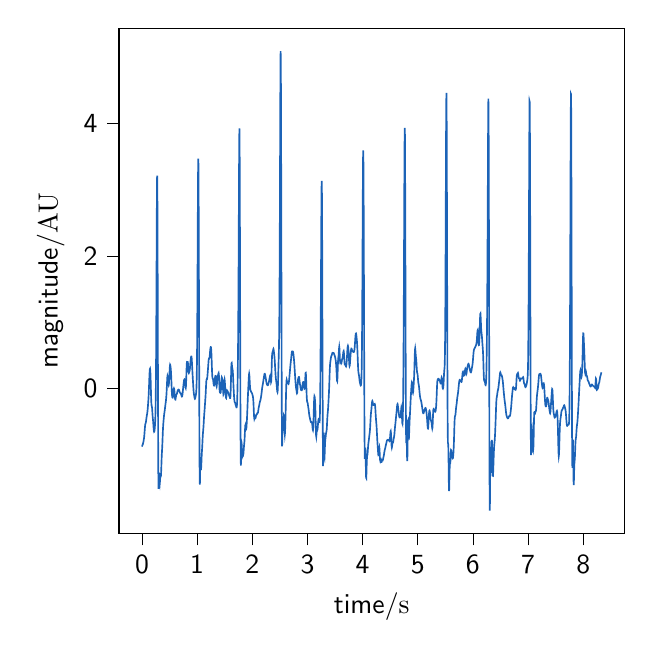
\begin{tikzpicture}
\pgfplotsset{
   every axis/.append style={
		font=\fontsize{10}{10}\sffamily},
	every non boxed x axis/.append style={
		x axis line style={->}
	},
	every non boxed y axis/.append style={
		y axis line style={->}
	},
	every non boxed z axis/.append style={
		z axis line style={->}
	}
}
\begin{axis}[
height=\figH,
tick align=outside,
tick pos=left,
width=\figW,
x grid style={white!69.0196078431373!black},
xlabel={time/$\si{\second}$},
xmin=-0.416499996185303, xmax=8.74649991989136,
xtick style={color=black},
y grid style={white!69.0196078431373!black},
ylabel={magnitude/\si{AU}},
ymin=-2.19102610318908, ymax=5.44248037929603,
ytick style={color=black},
ytick = {0, 2, 4},
yticklabels = {0, 2, 4},
xtick = {0, 1, 2, 3, 4, 5, 6, 7, 8},
xticklabels = {0, 1, 2, 3, 4, 5, 6, 7, 8},
]
\addplot [semithick, tud1b]
table {%
0 -0.875887141497869
0.00333333341404796 -0.865536337141689
0.00666666682809591 -0.858595100817909
0.00999999977648258 -0.853415151098276
0.0133333336561918 -0.847302777908773
0.0166666675359011 -0.838483188233128
0.0199999995529652 -0.827014618274032
0.0233333334326744 -0.814141066255638
0.0266666673123837 -0.800876020938007
0.0299999993294477 -0.787074836550384
0.0333333350718021 -0.771539655159133
0.0366666652262211 -0.752657329895357
0.0399999991059303 -0.728895399212196
0.0433333329856396 -0.699230123460934
0.0466666668653488 -0.663988016248374
0.0500000007450581 -0.625830282152597
0.0533333346247673 -0.589672740727012
0.0566666685044765 -0.560750886871006
0.0599999986588955 -0.541730633446391
0.0633333325386047 -0.530965146589033
0.0666666701436043 -0.523344752843231
0.0700000002980232 -0.51323090232774
0.0733333304524422 -0.49746606821868
0.0766666680574417 -0.47657927047917
0.0799999982118607 -0.453731190644993
0.0833333358168602 -0.432411973461108
0.0866666659712791 -0.41441578370085
0.0900000035762787 -0.399083941344306
0.0933333337306976 -0.383878052462684
0.0966666638851166 -0.36571019468006
0.100000001490116 -0.342333779829628
0.103333331644535 -0.313250244982893
0.106666669249535 -0.279750700268699
0.109999999403954 -0.243917352816445
0.113333337008953 -0.206869800675871
0.116666667163372 -0.167226294210774
0.119999997317791 -0.121105888317749
0.123333334922791 -0.064318441791777
0.126666665077209 0.00425707762818561
0.129999995231628 0.0804511091378703
0.133333340287209 0.155647019424894
0.136666670441628 0.220338536255665
0.140000000596046 0.267782066542253
0.143333330750465 0.294964283551946
0.146666660904884 0.300423457074161
0.150000005960464 0.281385552963128
0.153333336114883 0.233633937517347
0.156666666269302 0.155431496375307
0.159999996423721 0.053019052939979
0.16333332657814 -0.0572607445767631
0.16666667163372 -0.153754055660871
0.170000001788139 -0.219687932067678
0.173333331942558 -0.25227677877742
0.176666662096977 -0.263914902183291
0.180000007152557 -0.273982429075807
0.183333337306976 -0.296821293847915
0.186666667461395 -0.334319903116858
0.189999997615814 -0.377840610231282
0.193333327770233 -0.41700838351541
0.196666672825813 -0.448014742203807
0.200000002980232 -0.475279793488605
0.203333333134651 -0.506174163898777
0.20666666328907 -0.543953708250432
0.209999993443489 -0.584748205614136
0.213333338499069 -0.620365284084378
0.216666668653488 -0.643805510267837
0.219999998807907 -0.652842542742796
0.223333328962326 -0.649478864081552
0.226666674017906 -0.636750133853869
0.230000004172325 -0.615952226817687
0.233333334326744 -0.58601054348235
0.236666664481163 -0.544179319570119
0.239999994635582 -0.486011704955369
0.243333339691162 -0.40351353691533
0.246666669845581 -0.282459223243398
0.25 -0.101214829119763
0.253333330154419 0.166674890795714
0.256666660308838 0.544924873124507
0.259999990463257 1.04220094079474
0.263333320617676 1.63735823521966
0.266666680574417 2.26752191055716
0.270000010728836 2.82692373363091
0.273333340883255 3.183570676269
0.276666671037674 3.21454725649055
0.280000001192093 2.85105599986415
0.283333331346512 2.11612294641069
0.286666661500931 1.13569968367286
0.28999999165535 0.110386776169235
0.293333321809769 -0.749120337625778
0.296666651964188 -1.29899276174656
0.300000011920929 -1.51433973057888
0.303333342075348 -1.48656505746466
0.306666672229767 -1.36562247658502
0.310000002384186 -1.28041364107883
0.313333332538605 -1.28362557995072
0.316666662693024 -1.34916739902886
0.319999992847443 -1.41451656618655
0.323333323001862 -1.43321786246822
0.326666653156281 -1.40248668589536
0.330000013113022 -1.35395799886108
0.333333343267441 -1.32250369097587
0.33666667342186 -1.31958616584771
0.340000003576279 -1.32879940623903
0.343333333730698 -1.32218152212607
0.346666663885117 -1.28179343147776
0.349999994039536 -1.21059486412497
0.353333324193954 -1.12723533839218
0.356666654348373 -1.05142076127035
0.360000014305115 -0.991524325352889
0.363333344459534 -0.942210829352809
0.366666674613953 -0.891564360696037
0.370000004768372 -0.831019251092908
0.373333334922791 -0.760958000204326
0.376666665077209 -0.689209384936858
0.379999995231628 -0.624944925253096
0.383333325386047 -0.572974408199803
0.386666655540466 -0.532103432205657
0.389999985694885 -0.497706679031579
0.393333345651627 -0.465777860984432
0.396666675806046 -0.435297562544243
0.400000005960464 -0.407642199008429
0.403333336114883 -0.384185230495095
0.406666666269302 -0.364365299442755
0.409999996423721 -0.345719537110648
0.41333332657814 -0.325596570439038
0.416666656732559 -0.302966275892263
0.419999986886978 -0.278850921905718
0.423333346843719 -0.255162311681346
0.426666676998138 -0.23302164888738
0.430000007152557 -0.21189888627011
0.433333337306976 -0.189993503778215
0.436666667461395 -0.165106158057235
0.439999997615814 -0.135012154268154
0.443333327770233 -0.0973211751876249
0.446666657924652 -0.0498856166074955
0.449999988079071 0.00743321576302117
0.453333348035812 0.0704501875567022
0.456666678190231 0.129926400351453
0.46000000834465 0.17399352930913
0.463333338499069 0.193079847056378
0.466666668653488 0.184622062095589
0.469999998807907 0.154634347541741
0.473333328962326 0.115091880861028
0.476666659116745 0.078785920684215
0.479999989271164 0.0548767962710136
0.483333319425583 0.0475774434850373
0.486666679382324 0.0578198127383252
0.490000009536743 0.0855006198051027
0.493333339691162 0.129842918354458
0.496666669845581 0.187519508549643
0.5 0.250633703062952
0.503333330154419 0.307351444922048
0.506666660308838 0.34612321274929
0.509999990463257 0.36121971711779
0.513333320617676 0.355392869033127
0.516666650772095 0.336999555332697
0.519999980926514 0.3132307310723
0.523333311080933 0.284629076098725
0.526666641235352 0.245437042815145
0.529999971389771 0.18966431049206
0.533333361148834 0.118009887291545
0.536666691303253 0.0400095961909245
0.540000021457672 -0.0303949570821982
0.543333351612091 -0.0824886026598785
0.54666668176651 -0.113888293511427
0.550000011920929 -0.129623234245074
0.553333342075348 -0.136533133361934
0.556666672229767 -0.137793507204418
0.560000002384186 -0.131749480882231
0.563333332538605 -0.115313696914963
0.566666662693024 -0.0884818237469154
0.569999992847443 -0.0561154942043315
0.573333323001862 -0.0259676423161453
0.576666653156281 -0.00508155071455046
0.579999983310699 0.00258738603369817
0.583333313465118 -0.00371317424807828
0.586666643619537 -0.0226115534893837
0.589999973773956 -0.0513629847593556
0.593333303928375 -0.0858318336779662
0.596666693687439 -0.120388595442652
0.600000023841858 -0.148571717224037
0.603333353996277 -0.164749263435833
0.606666684150696 -0.166220845289498
0.610000014305115 -0.154633500406913
0.613333344459534 -0.135596810375793
0.616666674613953 -0.116251883892918
0.620000004768372 -0.101938099535553
0.623333334922791 -0.0939409286902931
0.626666665077209 -0.0897099184075719
0.629999995231628 -0.0852262315839721
0.633333325386047 -0.077744349998432
0.636666655540466 -0.0671040235525922
0.639999985694885 -0.0551119491399138
0.643333315849304 -0.0439285019393619
0.646666646003723 -0.034817435273832
0.649999976158142 -0.0279227810275729
0.653333306312561 -0.0227805261674254
0.656666696071625 -0.018909158644518
0.660000026226044 -0.0161259602748598
0.663333356380463 -0.0146375459340437
0.666666686534882 -0.0150103829354303
0.670000016689301 -0.0179625675844669
0.673333346843719 -0.0239144729762882
0.676666676998138 -0.0324877016264963
0.680000007152557 -0.0423488035979306
0.683333337306976 -0.0516468333706292
0.686666667461395 -0.0588519551104544
0.689999997615814 -0.0634571123664674
0.693333327770233 -0.0660885697082286
0.696666657924652 -0.0680218902517331
0.699999988079071 -0.0705182968912168
0.70333331823349 -0.0744303361675533
0.706666648387909 -0.0801888442168924
0.709999978542328 -0.0879134810088589
0.713333308696747 -0.0973264931216459
0.716666638851166 -0.107437615830622
0.720000028610229 -0.116323499073313
0.723333358764648 -0.121388387159172
0.726666688919067 -0.120161651382046
0.730000019073486 -0.111235709319022
0.733333349227905 -0.0947833375714119
0.736666679382324 -0.0723683188952416
0.740000009536743 -0.0462312440174947
0.743333339691162 -0.0185034452900454
0.746666669845581 0.00928120448915668
0.75 0.0362688835340226
0.753333330154419 0.0620391974357826
0.756666660308838 0.0861582122211824
0.759999990463257 0.107704247626327
0.763333320617676 0.125019820287377
0.766666650772095 0.13592591551999
0.769999980926514 0.138406273500978
0.773333311080933 0.131431905921665
0.776666641235352 0.115419626646094
0.779999971389771 0.0920671964418208
0.783333361148834 0.0639975760498883
0.786666691303253 0.0351749604843628
0.790000021457672 0.0123739159487039
0.793333351612091 0.00603092747886165
0.79666668176651 0.0276953351630084
0.800000011920929 0.0834571599447268
0.803333342075348 0.167237722779603
0.806666672229767 0.260107415808668
0.810000002384186 0.33836780399553
0.813333332538605 0.386068383758559
0.816666662693024 0.403139692688558
0.819999992847443 0.402891126966008
0.823333323001862 0.400639051441902
0.826666653156281 0.402213300417594
0.829999983310699 0.401141369044944
0.833333313465118 0.386202213365299
0.836666643619537 0.352639697609384
0.839999973773956 0.307689516567652
0.843333303928375 0.266258667657473
0.846666693687439 0.240861315802051
0.850000023841858 0.234147733378908
0.853333353996277 0.239440189395441
0.856666684150696 0.247777571271804
0.860000014305115 0.255137782090678
0.863333344459534 0.264329029712495
0.866666674613953 0.28103922354719
0.870000004768372 0.308128629969691
0.873333334922791 0.342919667384742
0.876666665077209 0.379115289243892
0.879999995231628 0.411108646069754
0.883333325386047 0.436924005429492
0.886666655540466 0.457648362751421
0.889999985694885 0.474279053788921
0.893333315849304 0.484897051574499
0.896666646003723 0.484600977286097
0.899999976158142 0.468322576011009
0.903333306312561 0.434397333358257
0.906666696071625 0.386238243832343
0.910000026226044 0.330896042902855
0.913333356380463 0.275504643426184
0.916666686534882 0.223997506611192
0.920000016689301 0.176159162393923
0.923333346843719 0.12940295272984
0.926666676998138 0.0818504597459218
0.930000007152557 0.0345131032130302
0.933333337306976 -0.00891884145536957
0.936666667461395 -0.0444777266648852
0.939999997615814 -0.0707267064822455
0.943333327770233 -0.0898311542747264
0.946666657924652 -0.105979660522414
0.949999988079071 -0.122257655715833
0.95333331823349 -0.138334263373805
0.956666648387909 -0.150749313740861
0.959999978542328 -0.155581138868669
0.963333308696747 -0.151440319520523
0.966666638851166 -0.140516849369451
0.970000028610229 -0.126919978867086
0.973333358764648 -0.113579024992096
0.976666688919067 -0.0999749258166286
0.980000019073486 -0.0821327583961944
0.983333349227905 -0.0541256762384238
0.986666679382324 -0.00859766247776855
0.990000009536743 0.0655058448613694
0.993333339691162 0.186571187468078
0.996666669845581 0.380861444646125
1 0.676123850716883
1.00333333015442 1.0888068902545
1.00666666030884 1.60997448475741
1.00999999046326 2.19620143393531
1.01333332061768 2.76973420547846
1.01666665077209 3.2293661437597
1.01999998092651 3.47084069735395
1.02333331108093 3.41265784321393
1.02666664123535 3.02049673219879
1.02999997138977 2.32301770962142
1.03333330154419 1.41396732495442
1.03666663169861 0.438124802146735
1.03999996185303 -0.439525656839587
1.04333329200745 -1.07817908013314
1.04666662216187 -1.40714347080811
1.04999995231628 -1.45203665162006
1.0533332824707 -1.32182372516928
1.05666661262512 -1.15653384342121
1.05999994277954 -1.06164317368797
1.06333339214325 -1.06680256660711
1.06666672229767 -1.13155391125921
1.07000005245209 -1.18892384626813
1.07333338260651 -1.19382608141186
1.07666671276093 -1.14481919924366
1.08000004291534 -1.07139797266127
1.08333337306976 -1.00430001235887
1.08666670322418 -0.954214884626847
1.0900000333786 -0.911961877075086
1.09333336353302 -0.863909601303213
1.09666669368744 -0.806341313522861
1.10000002384186 -0.747397428881696
1.10333335399628 -0.697947257352809
1.1066666841507 -0.661462011393874
1.11000001430511 -0.631644907967571
1.11333334445953 -0.598474958076723
1.11666667461395 -0.556352700017774
1.12000000476837 -0.507502399929264
1.12333333492279 -0.458794478172462
1.12666666507721 -0.41565614321127
1.12999999523163 -0.378332465959218
1.13333332538605 -0.3429475772329
1.13666665554047 -0.305592884815602
1.13999998569489 -0.26554681641202
1.1433333158493 -0.224994323837417
1.14666664600372 -0.185820459388817
1.14999997615814 -0.146573708647888
1.15333330631256 -0.102666378562667
1.15666663646698 -0.0502755138926265
1.1599999666214 0.00891994082302658
1.16333329677582 0.06637006957861
1.16666662693024 0.110680267276194
1.16999995708466 0.134740050673952
1.17333328723907 0.140778025584626
1.17666661739349 0.139398829438837
1.17999994754791 0.143183521092235
1.18333327770233 0.159542554960866
1.18666660785675 0.187865614573995
1.19000005722046 0.222455452562552
1.19333338737488 0.258224020154761
1.1966667175293 0.294243470355239
1.20000004768372 0.332416680022924
1.20333337783813 0.372958618658694
1.20666670799255 0.411310775025347
1.21000003814697 0.439892965917823
1.21333336830139 0.453687467388249
1.21666669845581 0.455001288449806
1.22000002861023 0.453190988605963
1.22333335876465 0.459230300901177
1.22666668891907 0.479108207664848
1.23000001907349 0.510786259478147
1.23333334922791 0.546516429729341
1.23666667938232 0.578285535895627
1.24000000953674 0.602094641665618
1.24333333969116 0.618083230419688
1.24666666984558 0.627025584005655
1.25 0.62663268909504
1.25333333015442 0.611032886708236
1.25666666030884 0.57397723541399
1.25999999046326 0.513362918732476
1.26333332061768 0.4340224262414
1.26666665077209 0.34725785239995
1.26999998092651 0.267412662348591
1.27333331108093 0.206791941814975
1.27666664123535 0.170859945402618
1.27999997138977 0.156036638663226
1.28333330154419 0.15171118542502
1.28666663169861 0.145829684731268
1.28999996185303 0.130946558049225
1.29333329200745 0.10714580853729
1.29666662216187 0.0804312228457887
1.29999995231628 0.0583248429699334
1.3033332824707 0.0459455611104447
1.30666661262512 0.0447514241876646
1.30999994277954 0.0536977448325843
1.31333339214325 0.070961021298824
1.31666672229767 0.0946693042276514
1.32000005245209 0.122492245686906
1.32333338260651 0.150959368468213
1.32666671276093 0.175326534461164
1.33000004291534 0.190236069425501
1.33333337306976 0.191021856446084
1.33666670322418 0.175340440332223
1.3400000333786 0.144614127584817
1.34333336353302 0.104643331909113
1.34666669368744 0.0649006930846071
1.35000002384186 0.0363553218696966
1.35333335399628 0.0280716076930717
1.3566666841507 0.0435008018170642
1.36000001430511 0.0782580297147202
1.36333334445953 0.121270717117589
1.36666667461395 0.159578942972602
1.37000000476837 0.184497060737484
1.37333333492279 0.195470817982115
1.37666666507721 0.199193867354026
1.37999999523163 0.204494806327571
1.38333332538605 0.215969510413167
1.38666665554047 0.229957832578668
1.38999998569489 0.235365950821711
1.3933333158493 0.219529736795442
1.39666664600372 0.176332259431787
1.39999997615814 0.111606391063023
1.40333330631256 0.0416483709948006
1.40666663646698 -0.015069278456509
1.4099999666214 -0.0479059453609105
1.41333329677582 -0.0590125659001357
1.41666662693024 -0.0597487871194399
1.41999995708466 -0.0610722515919687
1.42333328723907 -0.0648264391749134
1.42666661739349 -0.0623913060884964
1.42999994754791 -0.0418584689202295
1.43333327770233 0.00159977588100556
1.43666660785675 0.0601377355062037
1.44000005722046 0.116771163967309
1.44333338737488 0.155285387814791
1.4466667175293 0.169039668573238
1.45000004768372 0.162585820831454
1.45333337783813 0.145911423371782
1.45666670799255 0.12640121280479
1.46000003814697 0.10442725066556
1.46333336830139 0.0750975774265235
1.46666669845581 0.0343147347521321
1.47000002861023 -0.0151637395647076
1.47333335876465 -0.0617085903228231
1.47666668891907 -0.0886420747845565
1.48000001907349 -0.0824891159828105
1.48333334922791 -0.0412747448314186
1.48666667938232 0.0224428627945544
1.49000000953674 0.0865209652390874
1.49333333969116 0.129720604791661
1.49666666984558 0.141291723497402
1.5 0.123820718115638
1.50333333015442 0.0884107170089499
1.50666666030884 0.0464940274374431
1.50999999046326 0.00417968317406944
1.51333332061768 -0.0376611049897122
1.51666665077209 -0.0788928554814329
1.51999998092651 -0.11561545339321
1.52333331108093 -0.139792937883956
1.52666664123535 -0.143714982022483
1.52999997138977 -0.125914449477096
1.53333330154419 -0.093691735864822
1.53666663169861 -0.0599092640758961
1.53999996185303 -0.0361886581070759
1.54333329200745 -0.0273011460863871
1.54666662216187 -0.0303185883431201
1.54999995231628 -0.0383308121672734
1.5533332824707 -0.0454662019565407
1.55666661262512 -0.0497615096279066
1.55999994277954 -0.0526977716265685
1.56333339214325 -0.0567674446545972
1.56666672229767 -0.0633459267700835
1.57000005245209 -0.0721640232992769
1.57333338260651 -0.0820735744179
1.57666671276093 -0.0919967198679004
1.58000004291534 -0.10133728895191
1.58333337306976 -0.109962626216251
1.58666670322418 -0.118172772029272
1.5900000333786 -0.126621906508125
1.59333336353302 -0.135584060317973
1.59666669368744 -0.143145170784855
1.60000002384186 -0.143095876584079
1.60333335399628 -0.124634134814009
1.6066666841507 -0.0759619015506366
1.61000001430511 0.00843594750771337
1.61333334445953 0.120667642967176
1.61666667461395 0.23830938182353
1.62000000476837 0.332583200949089
1.62333333492279 0.382533128534092
1.62666666507721 0.386188761248929
1.62999999523163 0.360498457475665
1.63333332538605 0.329558246123603
1.63666665554047 0.309363609647412
1.63999998569489 0.299702611812668
1.6433333158493 0.287964064477477
1.64666664600372 0.260575319604124
1.64999997615814 0.212862587171953
1.65333330631256 0.150744918015074
1.65666663646698 0.084858267809818
1.6599999666214 0.0231968165148603
1.66333329677582 -0.031901546822386
1.66666662693024 -0.0814020335478003
1.66999995708466 -0.125435427946074
1.67333328723907 -0.161611360160415
1.67666661739349 -0.186946668907594
1.67999994754791 -0.201087358808668
1.68333327770233 -0.207617062049503
1.68666660785675 -0.21224370182346
1.69000005722046 -0.219415297878186
1.69333338737488 -0.230078123741805
1.6966667175293 -0.24215093452333
1.70000004768372 -0.253026675360611
1.70333337783813 -0.261882787798964
1.70666670799255 -0.269870835916956
1.71000003814697 -0.278029198306817
1.71333336830139 -0.284618706492846
1.71666669845581 -0.284076619428904
1.72000002861023 -0.268490365606683
1.72333335876465 -0.230402812048353
1.72666668891907 -0.164630220769698
1.73000001907349 -0.0676622114046866
1.73333334922791 0.0646556012181368
1.73666667938232 0.239173371732781
1.74000000953674 0.466016815914361
1.74333333969116 0.758022845987793
1.74666666984558 1.12919592473376
1.75 1.5902057727215
1.75333333015442 2.13793231830931
1.75666666030884 2.73961896466179
1.75999999046326 3.31948189981906
1.76333332061768 3.76052490785722
1.76666665077209 3.93032655570445
1.76999998092651 3.72664696382959
1.77333331108093 3.12473782786277
1.77666664123535 2.20299470222752
1.77999997138977 1.13105666989754
1.78333330154419 0.120677820555346
1.78666663169861 -0.643425776706095
1.78999996185303 -1.06527398870259
1.79333329200745 -1.16510010011257
1.79666662216187 -1.05895264247241
1.79999995231628 -0.89895573287861
1.8033332824707 -0.803760956222846
1.80666661262512 -0.814864530797629
1.80999994277954 -0.899165891339008
1.81333339214325 -0.98990234106451
1.81666672229767 -1.03600867979038
1.82000005245209 -1.02904217699009
1.82333338260651 -0.996143636394032
1.82666671276093 -0.9715623830339
1.83000004291534 -0.970804803567822
1.83333337306976 -0.984455785768526
1.83666670322418 -0.99132258036397
1.8400000333786 -0.976992701513143
1.84333336353302 -0.943093373744683
1.84666669368744 -0.902503492033173
1.85000002384186 -0.867080898860498
1.85333335399628 -0.838602210289044
1.8566666841507 -0.809056463635542
1.86000001430511 -0.768430175738488
1.86333334445953 -0.71328987115514
1.86666667461395 -0.650376431429952
1.87000000476837 -0.593693494883203
1.87333333492279 -0.557410186108015
1.87666666507721 -0.54855868540608
1.87999999523163 -0.563254463702576
1.88333332538605 -0.588432522129435
1.88666665554047 -0.608179028789561
1.88999998569489 -0.610947764139565
1.8933333158493 -0.59339315071104
1.89666664600372 -0.55903424969988
1.89999997615814 -0.513640588998087
1.90333330631256 -0.461103651097926
1.90666663646698 -0.402371818459443
1.9099999666214 -0.337264506934917
1.91333329677582 -0.267014896083767
1.91666662693024 -0.195273729320125
1.91999995708466 -0.126624971455005
1.92333328723907 -0.0636100160192452
1.92666661739349 -0.00482620609523607
1.92999994754791 0.0535622146982587
1.93333327770233 0.113193319405328
1.93666660785675 0.169250451667166
1.94000005722046 0.210643235024736
1.94333338737488 0.225510089727001
1.9466667175293 0.208564371415341
1.95000004768372 0.165104924045323
1.95333337783813 0.108888142514017
1.95666670799255 0.0554231836096967
1.96000003814697 0.0151434474908497
1.96333336830139 -0.00958848579010989
1.96666669845581 -0.0227351636649575
1.97000002861023 -0.0302768164151212
1.97333335876465 -0.0365327906901159
1.97666668891907 -0.0429817779405527
1.98000001907349 -0.0492657055272669
1.98333334922791 -0.0547900347625429
1.98666667938232 -0.059612625780623
1.99000000953674 -0.0643935581038599
1.99333333969116 -0.0699240485359148
1.99666666984558 -0.0767422566140625
2 -0.0849843266446215
2.00333333015442 -0.0944400188873331
2.00666666030884 -0.104879902187503
2.00999999046326 -0.116816687028209
2.01333332061768 -0.132603813072785
2.01666665077209 -0.157033614399894
2.01999998092651 -0.195956917987397
2.02333331108093 -0.252217581702415
2.02666664123535 -0.320854779768762
2.02999997138977 -0.387911768962729
2.03333330154419 -0.435907364652208
2.03666663169861 -0.453763744685664
2.03999996185303 -0.444216168094914
2.04333329200745 -0.422543633902594
2.04666662216187 -0.406904181013039
2.04999995231628 -0.407169849824455
2.0533332824707 -0.420207572561971
2.05666661262512 -0.434340148123991
2.05999994277954 -0.438812614996285
2.06333327293396 -0.430982368737287
2.06666660308838 -0.416567365726818
2.0699999332428 -0.403957374156497
2.07333326339722 -0.397721552776235
2.07666659355164 -0.396211134358717
2.07999992370605 -0.39434519353772
2.08333325386047 -0.388589350491168
2.08666658401489 -0.379863358751418
2.08999991416931 -0.37225978998849
2.09333324432373 -0.369012343231153
2.09666657447815 -0.369251310146841
2.09999990463257 -0.368228478734531
2.10333323478699 -0.360768057621963
2.10666656494141 -0.345125207906217
2.10999989509583 -0.324217761071179
2.11333322525024 -0.303388655787887
2.11666655540466 -0.286595194399279
2.11999988555908 -0.274011230900273
2.1233332157135 -0.262713503286943
2.1266667842865 -0.249600674660006
2.13000011444092 -0.234035913691726
2.13333344459534 -0.218156547584331
2.13666677474976 -0.204838285632737
2.14000010490417 -0.195180443169001
2.14333343505859 -0.187591712895934
2.14666676521301 -0.179064008852623
2.15000009536743 -0.167390456181079
2.15333342552185 -0.152451787969776
2.15666675567627 -0.135665797788485
2.16000008583069 -0.1183016872248
2.16333341598511 -0.100228745971121
2.16666674613953 -0.0801700837039878
2.17000007629395 -0.0571801769282828
2.17333340644836 -0.0320044912769634
2.17666673660278 -0.00707625288713934
2.1800000667572 0.0149361933611022
2.18333339691162 0.0328908273240206
2.18666672706604 0.0478509442917002
2.19000005722046 0.0621969450493868
2.19333338737488 0.0779392348453419
2.1966667175293 0.0955553227720457
2.20000004768372 0.114137144635103
2.20333337783813 0.132517281551719
2.20666670799255 0.150285381799394
2.21000003814697 0.167809471754703
2.21333336830139 0.185313998728443
2.21666669845581 0.201892125230093
2.22000002861023 0.215360061365712
2.22333335876465 0.223159439287878
2.22666668891907 0.223707112718751
2.23000001907349 0.217263448772761
2.23333334922791 0.205718607606179
2.23666667938232 0.191449724404873
2.24000000953674 0.176068027946333
2.24333333969116 0.159942475732543
2.24666666984558 0.142764827304435
2.25 0.124598994207226
2.25333333015442 0.106509025930374
2.25666666030884 0.0902501839916734
2.25999999046326 0.0772906636883603
2.26333332061768 0.0679690218102219
2.26666665077209 0.0614597266049956
2.26999998092651 0.0565410794388102
2.27333331108093 0.0525259958931383
2.27666664123535 0.0496641632828168
2.27999997138977 0.0488295978928572
2.28333330154419 0.0508534156648204
2.28666663169861 0.0560095489979679
2.28999996185303 0.0639288134180389
2.29333329200745 0.0738913832947003
2.29666662216187 0.0852377017100957
2.29999995231628 0.0976085638558005
2.3033332824707 0.110885491390782
2.30666661262512 0.12496639447562
2.30999994277954 0.139658894524545
2.31333327293396 0.154804809422617
2.31666660308838 0.170316861898062
2.3199999332428 0.185540579716032
2.32333326339722 0.197859606955782
2.32666659355164 0.201794864829197
2.32999992370605 0.190782320373519
2.33333325386047 0.162532987449236
2.33666658401489 0.125238219784462
2.33999991416931 0.0988566966079174
2.34333324432373 0.107349474533825
2.34666657447815 0.164525146801398
2.34999990463257 0.262920141037802
2.35333323478699 0.375014495402614
2.35666656494141 0.467683626870008
2.35999989509583 0.520580873683175
2.36333322525024 0.535847235421235
2.36666655540466 0.533038418089732
2.36999988555908 0.534013726341348
2.3733332157135 0.549067629886944
2.3766667842865 0.573259493302978
2.38000011444092 0.593471516217575
2.38333344459534 0.599221168326278
2.38666677474976 0.58900511896071
2.39000010490417 0.568811286568259
2.39333343505859 0.545753148370749
2.39666676521301 0.522640373997004
2.40000009536743 0.497255472050518
2.40333342552185 0.465671708436039
2.40666675567627 0.426024979975953
2.41000008583069 0.379763536913361
2.41333341598511 0.330294426765964
2.41666674613953 0.281102384171412
2.42000007629395 0.235033398923019
2.42333340644836 0.194505484948829
2.42666673660278 0.161321591063456
2.4300000667572 0.135593186610361
2.43333339691162 0.114823925401419
2.43666672706604 0.0945370310538347
2.44000005722046 0.0705107218651662
2.44333338737488 0.0411383800805402
2.4466667175293 0.008340141303955
2.45000004768372 -0.0230908992426462
2.45333337783813 -0.0464971119105264
2.45666670799255 -0.0539104151333926
2.46000003814697 -0.0369799987870421
2.46333336830139 0.0103270433818868
2.46666669845581 0.0877187220856888
2.47000002861023 0.186419349378253
2.47333335876465 0.29232427596631
2.47666668891907 0.394608848846949
2.48000001907349 0.495391889640244
2.48333334922791 0.614393985621708
2.48666667938232 0.785581614254429
2.49000000953674 1.04795467134898
2.49333333969116 1.43505097687755
2.49666666984558 1.96531517154667
2.5 2.63167444269695
2.50333333015442 3.38916664695455
2.50666666030884 4.14550059251382
2.50999999046326 4.76516277651422
2.51333332061768 5.09550281191035
2.51666665077209 5.01185475059209
2.51999998092651 4.46556459377635
2.52333331108093 3.51361797596392
2.52666664123535 2.31503915033076
2.52999997138977 1.09238324967638
2.53333330154419 0.0689084162363019
2.53666663169861 -0.599534474331843
2.53999996185303 -0.873591072925432
2.54333329200745 -0.837194358434997
2.54666662216187 -0.653008201413661
2.54999995231628 -0.484111072756471
2.5533332824707 -0.422428904223487
2.55666661262512 -0.463306397400438
2.55999994277954 -0.536794490016113
2.56333327293396 -0.56972760173654
2.56666660308838 -0.535812964884273
2.5699999332428 -0.46478529361536
2.57333326339722 -0.412877546565921
2.57666659355164 -0.421196687197802
2.57999992370605 -0.490943909575166
2.58333325386047 -0.587692680714621
2.58666658401489 -0.666024649592668
2.58999991416931 -0.69501898052832
2.59333324432373 -0.669033073945175
2.59666657447815 -0.601118001812538
2.59999990463257 -0.508153704762567
2.60333323478699 -0.400163855207102
2.60666656494141 -0.280545920952473
2.60999989509583 -0.154175619431556
2.61333322525024 -0.0340091479779454
2.61666655540466 0.0611880304080931
2.61999988555908 0.11691194020042
2.6233332157135 0.132415796509645
2.6266667842865 0.121558037562367
2.63000011444092 0.104178172026935
2.63333344459534 0.0946406284853505
2.63666677474976 0.0956689699689203
2.64000010490417 0.100685824972091
2.64333343505859 0.101374925733245
2.64666676521301 0.0942866683145578
2.65000009536743 0.0824378522412224
2.65333342552185 0.0723177632955109
2.65666675567627 0.0696619487455068
2.66000008583069 0.0770428386119459
2.66333341598511 0.0939744966809892
2.66666674613953 0.118293241281255
2.67000007629395 0.147397368039813
2.67333340644836 0.178916474323181
2.67666673660278 0.211114463414231
2.6800000667572 0.24317391572585
2.68333339691162 0.275069549201828
2.68666672706604 0.306875990125372
2.69000005722046 0.338027088043739
2.69333338737488 0.36735495405715
2.6966667175293 0.394089040223601
2.70000004768372 0.418920168986468
2.70333337783813 0.443894030764588
2.70666670799255 0.470815457756357
2.71000003814697 0.499277293341339
2.71333336830139 0.526046648863765
2.71666669845581 0.546663611763221
2.72000002861023 0.558326846697419
2.72333335876465 0.561896115230646
2.72666668891907 0.561289750677401
2.73000001907349 0.560539024510055
2.73333334922791 0.560734026636276
2.73666667938232 0.559306095348713
2.74000000953674 0.552201343734853
2.74333333969116 0.537077723827538
2.74666666984558 0.514851441701949
2.75 0.488447890365771
2.75333333015442 0.460075229206979
2.75666666030884 0.429527101584505
2.75999999046326 0.394941791138834
2.76333332061768 0.355152855166251
2.76666665077209 0.311353718876772
2.76999998092651 0.266523320063201
2.77333331108093 0.223226404644317
2.77666664123535 0.181970935935086
2.77999997138977 0.141759085483942
2.78333330154419 0.102285485229115
2.78666663169861 0.065509251796718
2.78999996185303 0.0347738640281833
2.79333329200745 0.0119477602323362
2.79666662216187 -0.00486070788413676
2.79999995231628 -0.02052824024314
2.8033332824707 -0.0389498317679854
2.80666661262512 -0.0586162440090135
2.80999994277954 -0.0714986686205709
2.81333327293396 -0.0670384997112259
2.81666660308838 -0.0391972158539283
2.8199999332428 0.00832997376103907
2.82333326339722 0.0629288657818644
2.82666659355164 0.109879808686921
2.82999992370605 0.140506787410825
2.83333325386047 0.155810047514086
2.83666658401489 0.163195318327113
2.83999991416931 0.169290023170989
2.84333324432373 0.174687413544922
2.84666657447815 0.174500032616148
2.84999990463257 0.163638360095332
2.85333323478699 0.14198622554013
2.85666656494141 0.115123107147116
2.85999989509583 0.0902816435898959
2.86333322525024 0.0712346750842457
2.86666655540466 0.0564207973830243
2.86999988555908 0.0415539521977447
2.8733332157135 0.0240885178417944
2.8766667842865 0.00558954348273771
2.88000011444092 -0.00979188119044017
2.88333344459534 -0.0190412837030638
2.88666677474976 -0.022743226206529
2.89000010490417 -0.0241402055854952
2.89333343505859 -0.0257089056732832
2.89666676521301 -0.0263399237106661
2.90000009536743 -0.0217135947936586
2.90333342552185 -0.00776113341494077
2.90666675567627 0.0155632076641549
2.91000008583069 0.0433456290365326
2.91333341598511 0.0684673435481661
2.91666674613953 0.085860760833163
2.92000007629395 0.0948901023836352
2.92333340644836 0.0981596781509588
2.92666673660278 0.0980892931107653
2.9300000667572 0.0943348901692429
2.93333339691162 0.0841927826933946
2.93666672706604 0.0655455490776453
2.94000005722046 0.0399968548388702
2.94333338737488 0.0139864225805568
2.9466667175293 -0.00272752714331015
2.95000004768372 -0.000400352179388899
2.95333337783813 0.0267870610740789
2.95666670799255 0.0773936496374473
2.96000003814697 0.141275460250868
2.96333336830139 0.201369141441277
2.96666669845581 0.238914492463086
2.97000002861023 0.240210800087827
2.97333335876465 0.201648240771697
2.97666668891907 0.13063903932763
2.98000001907349 0.0424835022122055
2.98333334922791 -0.0449680469239665
2.98666667938232 -0.11679584119065
2.99000000953674 -0.165147221557843
2.99333333969116 -0.1908654513244
2.99666666984558 -0.201822465988811
3 -0.208414352023516
3.00333333015442 -0.218430872752586
3.00666666030884 -0.234196920976819
3.00999999046326 -0.253472770874155
3.01333332061768 -0.27294889591834
3.01666665077209 -0.291415855330275
3.01999998092651 -0.31029402723532
3.02333331108093 -0.331598274974206
3.02666664123535 -0.355497914681115
3.02999997138977 -0.379698459427116
3.03333330154419 -0.401059697512615
3.03666663169861 -0.417903065091461
3.03999996185303 -0.431025839932614
3.04333329200745 -0.442727754858952
3.04666662216187 -0.454881525222652
3.04999995231628 -0.467723415951244
3.0533332824707 -0.480170216096911
3.05666661262512 -0.491019983791562
3.05999994277954 -0.499742943322398
3.06333327293396 -0.506249679355096
3.06666660308838 -0.510250916921944
3.0699999332428 -0.51129390977156
3.07333326339722 -0.509778652547116
3.07666659355164 -0.508041132525074
3.07999992370605 -0.510220207869846
3.08333325386047 -0.520521818706271
3.08666658401489 -0.540820651076391
3.08999991416931 -0.569068652927823
3.09333324432373 -0.599298352568956
3.09666657447815 -0.622868272547581
3.09999990463257 -0.630123985413759
3.10333323478699 -0.612187685344127
3.10666656494141 -0.563316902065684
3.10999989509583 -0.483999701307538
3.11333322525024 -0.383480311417677
3.11666655540466 -0.279170643493543
3.11999988555908 -0.191370985238593
3.1233332157135 -0.135078494892511
3.1266667842865 -0.113788215408941
3.13000011444092 -0.119872212092854
3.13333344459534 -0.141919137811584
3.13666677474976 -0.174285724111676
3.14000010490417 -0.221822151457123
3.14333343505859 -0.295268866483807
3.14666676521301 -0.399354367528863
3.15000009536743 -0.522201224387768
3.15333342552185 -0.635624193731377
3.15666675567627 -0.708670748267291
3.16000008583069 -0.725976680017741
3.16333341598511 -0.697453380892829
3.16666674613953 -0.651683707429496
3.17000007629395 -0.617708403151006
3.17333340644836 -0.608349932525482
3.17666673660278 -0.616145938459031
3.1800000667572 -0.622820689455336
3.18333339691162 -0.613672673238035
3.18666672706604 -0.586354065952914
3.19000005722046 -0.549431332056529
3.19333338737488 -0.514203589302004
3.1966667175293 -0.4873066984085
3.20000004768372 -0.469381093946691
3.20333337783813 -0.459114208613253
3.20666670799255 -0.457367645874993
3.21000003814697 -0.466596971054925
3.21333336830139 -0.485696462124699
3.21666669845581 -0.505051846941916
3.22000002861023 -0.506491527381181
3.22333335876465 -0.468214199820374
3.22666668891907 -0.370460981275603
3.23000001907349 -0.198101648361052
3.23333334922791 0.0593719825881324
3.23666667938232 0.406826197078259
3.24000000953674 0.839473781088635
3.24333333969116 1.33815110691935
3.24666666984558 1.86762507986065
3.25 2.37845142425396
3.25333333015442 2.80929815863066
3.25666666030884 3.0881539229175
3.25999999046326 3.13710543047284
3.26333332061768 2.88928649381105
3.26666665077209 2.32089630284494
3.26999998092651 1.48635242990979
3.27333331108093 0.531290957652404
3.27666664123535 -0.33935627525125
3.27999997138977 -0.936807283312706
3.28333330154419 -1.17260090977042
3.28666663169861 -1.10024044843174
3.28999996185303 -0.882766091442225
3.29333329200745 -0.701951493585938
3.29666662216187 -0.665026174981005
3.29999995231628 -0.765657368139615
3.3033332824707 -0.916312839595151
3.30666661262512 -1.02054012369538
3.30999994277954 -1.03261718231918
3.31333327293396 -0.970212937342081
3.31666660308838 -0.884027230001738
3.3199999332428 -0.816021773772791
3.32333326339722 -0.777339934860569
3.32666659355164 -0.754811963880201
3.32999992370605 -0.732072544283951
3.33333325386047 -0.704727363183781
3.33666658401489 -0.679596258276048
3.33999991416931 -0.663457908162929
3.34333324432373 -0.653836549704107
3.34666657447815 -0.639737709472139
3.34999990463257 -0.610342762311168
3.35333323478699 -0.563454947070595
3.35666656494141 -0.506933722215979
3.35999989509583 -0.452748038208772
3.36333322525024 -0.408849235512082
3.36666655540466 -0.374875252251351
3.36999988555908 -0.344045756223964
3.3733332157135 -0.308896684112378
3.3766667842865 -0.266219411332407
3.38000011444092 -0.217866050611115
3.38333344459534 -0.167481830161568
3.38666677474976 -0.116153348850914
3.39000010490417 -0.0605756812180444
3.39333343505859 0.00458819010829807
3.39666676521301 0.0816862621723436
3.40000009536743 0.166246347678764
3.40333342552185 0.247719346854398
3.40666675567627 0.314860856381272
3.41000008583069 0.362065355162112
3.41333341598511 0.39200178390186
3.41666674613953 0.412737512642934
3.42000007629395 0.431818905512192
3.42333340644836 0.45187035593793
3.42666673660278 0.47061013320177
3.4300000667572 0.48447406008647
3.43333339691162 0.492459273046748
3.43666672706604 0.497182913868165
3.44000005722046 0.502752291877259
3.44333338737488 0.511550953525384
3.4466667175293 0.522590376038101
3.45000004768372 0.532548631561664
3.45333337783813 0.538447040327916
3.45666670799255 0.539792263595351
3.46000003814697 0.538634544843591
3.46333336830139 0.53771058394758
3.46666669845581 0.538270590644209
3.47000002861023 0.539287106827494
3.47333335876465 0.538532382898865
3.47666668891907 0.534506480478774
3.48000001907349 0.527598034101173
3.48333334922791 0.519604179252131
3.48666667938232 0.512153759870485
3.49000000953674 0.505445855446559
3.49333333969116 0.498322178419293
3.49666666984558 0.489454910828097
3.5 0.478479220936227
3.50333333015442 0.466035939092836
3.50666666030884 0.452727114776325
3.50999999046326 0.43796968596085
3.51333332061768 0.41977551468153
3.51666665077209 0.395564289116419
3.51999998092651 0.363172235756821
3.52333331108093 0.321337477920545
3.52666664123535 0.270110903250461
3.52999997138977 0.212380177632865
3.53333330154419 0.15644808618374
3.53666663169861 0.116989234515893
3.53999996185303 0.110888411879448
3.54333329200745 0.147961870574907
3.54666662216187 0.22229501983975
3.54999995231628 0.31199909828628
3.5533332824707 0.390043543763161
3.55666661262512 0.439921008796896
3.55999994277954 0.464986611224657
3.56333327293396 0.484087397220949
3.56666660308838 0.515997503402101
3.5699999332428 0.563703530338934
3.57333326339722 0.610249601738119
3.57666659355164 0.629800108795569
3.57999992370605 0.606311286852377
3.58333325386047 0.546113644031272
3.58666658401489 0.474932617195049
3.58999991416931 0.421569929959038
3.59333324432373 0.400397364327794
3.59666657447815 0.405052354421041
3.59999990463257 0.416536887078742
3.60333323478699 0.418206219852869
3.60666656494141 0.406266615944977
3.60999989509583 0.389402977907759
3.61333322525024 0.379952150318597
3.61666655540466 0.384498006355448
3.61999988555908 0.400521890637165
3.6233332157135 0.420039730116552
3.6266667842865 0.436060864676399
3.63000011444092 0.446744321126809
3.63333344459534 0.455030341209563
3.63666677474976 0.465282738893171
3.64000010490417 0.480157477012571
3.64333343505859 0.499709813196601
3.64666676521301 0.522189622068485
3.65000009536743 0.544564298480215
3.65333342552185 0.561922043910438
3.65666675567627 0.567253662924444
3.66000008583069 0.55374426622456
3.66333341598511 0.519332230535773
3.66666674613953 0.470183341154458
3.67000007629395 0.419450230470391
3.67333340644836 0.381064219480687
3.67666673660278 0.362407973834899
3.6800000667572 0.360863670901561
3.68333339691162 0.366472305643918
3.68666672706604 0.368624424587067
3.69000005722046 0.362193267844639
3.69333338737488 0.349463936012346
3.6966667175293 0.337504003500707
3.70000004768372 0.333573402905296
3.70333337783813 0.341764411218074
3.70666670799255 0.362404543779856
3.71000003814697 0.393564972210853
3.71333336830139 0.432879500212421
3.71666669845581 0.478177036106753
3.72000002861023 0.526659157098008
3.72333335876465 0.573714014664006
3.72666668891907 0.612989491563571
3.73000001907349 0.638373552208709
3.73333334922791 0.646624917486269
3.73666667938232 0.638411280927718
3.74000000953674 0.61676189597259
3.74333333969116 0.584424573757342
3.74666666984558 0.542755114576146
3.75 0.493236059428671
3.75333333015442 0.440041311019531
3.75666666030884 0.390937995624084
3.75999999046326 0.355245772950404
3.76333332061768 0.340053573542217
3.76666665077209 0.347215867005694
3.76999998092651 0.372958729558515
3.77333331108093 0.410073358416282
3.77666664123535 0.451126639847444
3.77999997138977 0.490799626085784
3.78333330154419 0.526351523113726
3.78666663169861 0.55655478756501
3.78999996185303 0.580335638742344
3.79333329200745 0.596274668897892
3.79666662216187 0.603262245359944
3.79999995231628 0.601643098680289
3.8033332824707 0.593796815116042
3.80666661262512 0.583517578770502
3.80999994277954 0.574447103625465
3.81333327293396 0.568532016572313
3.81666660308838 0.565501217716002
3.8199999332428 0.563656530569251
3.82333326339722 0.561346080801882
3.82666659355164 0.558055429248909
3.82999992370605 0.554460504906949
3.83333325386047 0.551680309170487
3.83666658401489 0.550548676045928
3.83999991416931 0.551515418167572
3.84333324432373 0.55510468372235
3.84666657447815 0.562411426691893
3.84999990463257 0.575190643010504
3.85333323478699 0.595389840437091
3.85666656494141 0.624226099067276
3.85999989509583 0.661175729777048
3.86333322525024 0.703462311611902
3.86666655540466 0.746451353290101
3.86999988555908 0.784782430527471
3.8733332157135 0.81366477832425
3.8766667842865 0.829902274107364
3.88000011444092 0.83252784809727
3.88333344459534 0.822928048450969
3.88666677474976 0.804192535945563
3.89000010490417 0.779649876921464
3.89333343505859 0.751163179488282
3.89666676521301 0.718142981376963
3.90000009536743 0.677916205471806
3.90333342552185 0.627331343325887
3.90666675567627 0.564915415495825
3.91000008583069 0.492731388365853
3.91333341598511 0.417042373644285
3.91666674613953 0.346987639574148
3.92000007629395 0.29122204194393
3.92333340644836 0.253908559669596
3.92666673660278 0.232496106638142
3.9300000667572 0.219065540276753
3.93333339691162 0.204741419917274
3.93666672706604 0.184427306782841
3.94000005722046 0.158810215130868
3.94333338737488 0.132562456716851
3.9466667175293 0.110404982942114
3.95000004768372 0.0940225242184781
3.95333337783813 0.0817993539453425
3.95666670799255 0.0710068723666291
3.96000003814697 0.0603971706365103
3.96333336830139 0.0513121615494411
3.96666669845581 0.0469660086632557
3.97000002861023 0.0511321908485887
3.97333335876465 0.067984503287679
3.97666668891907 0.104063166578876
3.98000001907349 0.171668984850608
3.98333334922791 0.291265091334595
3.98666667938232 0.489834464704361
3.99000000953674 0.793446992095693
3.99333333969116 1.21517171309742
3.99666666984558 1.74238594083529
4 2.32894822492227
4.003333568573 2.89698281705333
4.00666666030884 3.35014530817212
4.01000022888184 3.59562444489653
4.01333332061768 3.56764843001015
4.01666688919067 3.24421803555542
4.01999998092651 2.65280841003721
4.02333354949951 1.86664425500515
4.02666664123535 0.995000545773614
4.03000020980835 0.167144760690646
4.03333330154419 -0.493915985314813
4.03666687011719 -0.906856115213134
4.03999996185303 -1.06330750091176
4.04333353042603 -1.03419592196935
4.04666662216187 -0.93949199869923
4.05000019073486 -0.892551352543453
4.0533332824707 -0.949184254782903
4.0566668510437 -1.0904393002812
4.05999994277954 -1.24675009284665
4.06333351135254 -1.34539941000406
4.06666660308838 -1.35124652540582
4.07000017166138 -1.27887349006754
4.07333326339722 -1.17469948191386
4.07666683197021 -1.08543201857859
4.07999992370605 -1.03389485212255
4.08333349227905 -1.01437866497952
4.08666658401489 -1.00531237398991
4.09000015258789 -0.987228934898591
4.09333324432373 -0.953863218658036
4.09666681289673 -0.91166838723995
4.09999990463257 -0.871517388089936
4.10333347320557 -0.840182543541628
4.10666656494141 -0.817136377932358
4.1100001335144 -0.797199189913423
4.11333322525024 -0.77558445955996
4.11666679382324 -0.751202862361448
4.11999988555908 -0.726263155857442
4.12333345413208 -0.703179719934575
4.12666654586792 -0.68151303156464
4.13000011444092 -0.657303650064653
4.13333320617676 -0.625298278572122
4.13666677474976 -0.582560013094443
4.1399998664856 -0.531016839059343
4.14333343505859 -0.477116025800486
4.14666652679443 -0.428557433226875
4.15000009536743 -0.390042380093111
4.15333318710327 -0.360801751949213
4.15666675567627 -0.33560069874187
4.15999984741211 -0.308542409149233
4.16333341598511 -0.277067663549422
4.16666650772095 -0.243575400009595
4.17000007629395 -0.213927114095083
4.17333316802979 -0.194144696618309
4.17666673660278 -0.187400811284223
4.17999982833862 -0.192772566644758
4.18333339691162 -0.206012264089611
4.18666648864746 -0.221603599461621
4.19000005722046 -0.234955081094326
4.1933331489563 -0.243734672860705
4.1966667175293 -0.247918532283362
4.19999980926514 -0.248822136390431
4.20333337783813 -0.247841403997394
4.20666646957397 -0.245640004657598
4.21000003814697 -0.242168123908307
4.21333312988281 -0.23745469802703
4.21666669845581 -0.232745897322306
4.21999979019165 -0.231284112650728
4.22333335876465 -0.237942027360797
4.22666645050049 -0.257347191696599
4.23000001907349 -0.291164008015746
4.23333311080933 -0.336257158554761
4.23666667938232 -0.385460601569419
4.23999977111816 -0.431109028832106
4.24333333969116 -0.469303230587929
4.246666431427 -0.5019536848467
4.25 -0.535052804752185
4.253333568573 -0.574414742840582
4.25666666030884 -0.621978046965894
4.26000022888184 -0.675111419687822
4.26333332061768 -0.728890745572542
4.26666688919067 -0.779286423891386
4.26999998092651 -0.825111623312375
4.27333354949951 -0.867865503304213
4.27666664123535 -0.909789880723383
4.28000020980835 -0.951027920264395
4.28333330154419 -0.987258873419405
4.28666687011719 -1.00971882133284
4.28999996185303 -1.00911153043411
4.29333353042603 -0.982581357826715
4.29666662216187 -0.939553565138014
4.30000019073486 -0.900920546924492
4.3033332824707 -0.889468362673496
4.3066668510437 -0.916315718830395
4.30999994277954 -0.972845175870564
4.31333351135254 -1.03498953561961
4.31666660308838 -1.07782356502769
4.32000017166138 -1.09039120322501
4.32333326339722 -1.08046158476531
4.32666683197021 -1.06665576638536
4.32999992370605 -1.06463101419047
4.33333349227905 -1.07750329070544
4.33666658401489 -1.09639142358818
4.34000015258789 -1.10901717894615
4.34333324432373 -1.10899890517842
4.34666681289673 -1.0992562936447
4.34999990463257 -1.08825002541715
4.35333347320557 -1.08303727955437
4.35666656494141 -1.08460364416105
4.3600001335144 -1.08830013559877
4.36333322525024 -1.08810653392437
4.36666679382324 -1.08101109727458
4.36999988555908 -1.06841838157656
4.37333345413208 -1.05416964284235
4.37666654586792 -1.04124061254313
4.38000011444092 -1.02975811326794
4.38333320617676 -1.01756505066202
4.38666677474976 -1.00249470947182
4.3899998664856 -0.984378282549898
4.39333343505859 -0.965281259278584
4.39666652679443 -0.94797243157787
4.40000009536743 -0.933952677458662
4.40333318710327 -0.922574878318969
4.40666675567627 -0.911822303909782
4.40999984741211 -0.899986051380159
4.41333341598511 -0.886842552105737
4.41666650772095 -0.87345791710462
4.42000007629395 -0.860949730603928
4.42333316802979 -0.84938057375926
4.42666673660278 -0.837750750035001
4.42999982833862 -0.825043988104292
4.43333339691162 -0.811377281286329
4.43666648864746 -0.79826048909905
4.44000005722046 -0.787740144706891
4.4433331489563 -0.781092555358486
4.4466667175293 -0.778042543252229
4.44999980926514 -0.777037118410363
4.45333337783813 -0.776304313764108
4.45666646957397 -0.774900144261098
4.46000003814697 -0.77304706318938
4.46333312988281 -0.771656705083012
4.46666669845581 -0.77153622762405
4.46999979019165 -0.772949419011562
4.47333335876465 -0.77580408341323
4.47666645050049 -0.780067518314174
4.48000001907349 -0.785679914466175
4.48333311080933 -0.791687462082763
4.48666667938232 -0.795284193568646
4.48999977111816 -0.791978073319736
4.49333333969116 -0.777449174040977
4.496666431427 -0.750278261606785
4.5 -0.713895371339981
4.503333568573 -0.676573057190023
4.50666666030884 -0.649432791452283
4.51000022888184 -0.643143392283088
4.51333332061768 -0.664090878142032
4.51666688919067 -0.711003173185828
4.51999998092651 -0.77360715447855
4.52333354949951 -0.835008254814628
4.52666664123535 -0.878006899368809
4.53000020980835 -0.892801789783331
4.53333330154419 -0.881604255547298
4.53666687011719 -0.856815293850054
4.53999996185303 -0.833470460033883
4.54333353042603 -0.82072266753348
4.54666662216187 -0.81787613729942
4.55000019073486 -0.817156006648944
4.5533332824707 -0.810568128666579
4.5566668510437 -0.795592821536727
4.55999994277954 -0.775886710412532
4.56333351135254 -0.757243561710024
4.56666660308838 -0.742502897717518
4.57000017166138 -0.729402645858591
4.57333326339722 -0.7126731170785
4.57666683197021 -0.688328504658791
4.57999992370605 -0.656692878627259
4.58333349227905 -0.622026279380589
4.58666658401489 -0.589377738299779
4.59000015258789 -0.561257828802045
4.59333324432373 -0.536529870438826
4.59666681289673 -0.511993298288748
4.59999990463257 -0.485124650081152
4.60333347320557 -0.455809872329964
4.60666656494141 -0.425910981795735
4.6100001335144 -0.397264650129088
4.61333322525024 -0.369905620498129
4.61666679382324 -0.342097329171139
4.61999988555908 -0.312291945889522
4.62333345413208 -0.281519333798417
4.62666654586792 -0.254190837327128
4.63000011444092 -0.236374124132067
4.63333320617676 -0.232489494395102
4.63666677474976 -0.242653682094625
4.6399998664856 -0.262558872481561
4.64333343505859 -0.286036216406676
4.64666652679443 -0.308556842406089
4.65000009536743 -0.329240537515338
4.65333318710327 -0.350015327401297
4.65666675567627 -0.372690603359851
4.65999984741211 -0.396319045288466
4.66333341598511 -0.417029907706746
4.66666650772095 -0.430559855845286
4.67000007629395 -0.435487424106397
4.67333316802979 -0.434497201538598
4.67666673660278 -0.43245532313226
4.67999982833862 -0.432550575762238
4.68333339691162 -0.43333360256102
4.68666648864746 -0.428966654097152
4.69000005722046 -0.412794237017649
4.6933331489563 -0.382152060891726
4.6966667175293 -0.341678950020015
4.69999980926514 -0.303340956292614
4.70333337783813 -0.282802463335207
4.70666646957397 -0.293012812801486
4.71000003814697 -0.337257398062328
4.71333312988281 -0.405277986892967
4.71666669845581 -0.475647758540169
4.71999979019165 -0.52402063540466
4.72333335876465 -0.532112699222892
4.72666645050049 -0.490895276712924
4.73000001907349 -0.395890466482541
4.73333311080933 -0.239343905491185
4.73666667938232 -0.00691480522243471
4.73999977111816 0.317650284689552
4.74333333969116 0.743559117082608
4.746666431427 1.2663156436878
4.75 1.86572848792382
4.753333568573 2.50465525269986
4.75666666030884 3.12408326266884
4.76000022888184 3.63751350127222
4.76333332061768 3.93567154411179
4.76666688919067 3.91160730867759
4.76999998092651 3.50383060774537
4.77333354949951 2.73897840926502
4.77666664123535 1.74753666543309
4.78000020980835 0.734153348577734
4.78333330154419 -0.093327512289321
4.78666687011719 -0.605958863842677
4.78999996185303 -0.803721139617222
4.79333353042603 -0.802509897241943
4.79666662216187 -0.762029610487838
4.80000019073486 -0.795702818469155
4.8033332824707 -0.916433189108252
4.8066668510437 -1.04882745206918
4.80999994277954 -1.09463508797875
4.81333351135254 -1.00492584794792
4.81666660308838 -0.812421748621792
4.82000017166138 -0.60793196684254
4.82333326339722 -0.48248539422184
4.82666683197021 -0.47570626047861
4.82999992370605 -0.561234936377547
4.83333349227905 -0.672106615169184
4.83666658401489 -0.743918790664919
4.84000015258789 -0.747018724990383
4.84333324432373 -0.691636293043592
4.84666681289673 -0.609870052718433
4.84999990463257 -0.531327964840585
4.85333347320557 -0.468454515092525
4.85666656494141 -0.417069010513036
4.8600001335144 -0.366663498284967
4.86333322525024 -0.310666959728185
4.86666679382324 -0.250058397124247
4.86999988555908 -0.190207407981577
4.87333345413208 -0.135454165410176
4.87666654586792 -0.0861664932417902
4.88000011444092 -0.0399160487107228
4.88333320617676 0.00495522042088604
4.88666677474976 0.0463988290314936
4.8899998664856 0.0783950779919977
4.89333343505859 0.0934919314373371
4.89666652679443 0.0867401351526283
4.90000009536743 0.0589813743255291
4.90333318710327 0.0177894085216916
4.90666675567627 -0.0244898056595996
4.90999984741211 -0.0547917273215516
4.91333341598511 -0.0638178688970965
4.91666650772095 -0.0491622049207015
4.92000007629395 -0.0156639549502764
4.92333316802979 0.0275932745004725
4.92666673660278 0.0727385025595772
4.92999982833862 0.118344442385512
4.93333339691162 0.170866178448488
4.93666648864746 0.240120292101518
4.94000005722046 0.330464758907691
4.9433331489563 0.433397484551727
4.9466667175293 0.527906007102139
4.94999980926514 0.590218794347495
4.95333337783813 0.607372948724495
4.95666646957397 0.585088120490113
4.96000003814697 0.543727412074364
4.96333312988281 0.504753122202381
4.96666669845581 0.477449954244782
4.96999979019165 0.455644871915131
4.97333335876465 0.42629694180476
4.97666645050049 0.382423744846854
4.98000001907349 0.32976476747798
4.98333311080933 0.282330862474435
4.98666667938232 0.251325519880408
4.98999977111816 0.236829227363632
4.99333333969116 0.228512253592066
4.996666431427 0.213926036999047
5 0.187325964097992
5.003333568573 0.152534470117539
5.00666666030884 0.118679489061064
5.01000022888184 0.092971173799563
5.01333332061768 0.0760861218993628
5.01666688919067 0.0628786635556774
5.01999998092651 0.0468563475985828
5.02333354949951 0.0245133949337061
5.02666664123535 -0.0034068534839912
5.03000020980835 -0.0336984747104352
5.03333330154419 -0.0632639881647134
5.03666687011719 -0.0903366035898167
5.03999996185303 -0.114074675577487
5.04333353042603 -0.133784205961097
5.04666662216187 -0.148925259731238
5.05000019073486 -0.159825677048604
5.0533332824707 -0.168124416577935
5.0566668510437 -0.176236578014451
5.05999994277954 -0.186143146515854
5.06333351135254 -0.198504075567726
5.06666660308838 -0.212822517995503
5.07000017166138 -0.228421656878257
5.07333326339722 -0.245252546962618
5.07666683197021 -0.263767505551257
5.07999992370605 -0.284069499976185
5.08333349227905 -0.305272419334124
5.08666658401489 -0.325719294954757
5.09000015258789 -0.343766083619279
5.09333324432373 -0.358313040766438
5.09666681289673 -0.368685058757315
5.09999990463257 -0.374263908397828
5.10333347320557 -0.374525610620044
5.10666656494141 -0.369592795257433
5.1100001335144 -0.360721419462254
5.11333322525024 -0.350071488605869
5.11666679382324 -0.339745742210991
5.11999988555908 -0.330788321537844
5.12333345413208 -0.322934554577661
5.12666654586792 -0.315300983167105
5.13000011444092 -0.307449553134182
5.13333320617676 -0.300007828482576
5.13666677474976 -0.294453610055545
5.1399998664856 -0.292359817934751
5.14333343505859 -0.29474717438671
5.14666652679443 -0.301956825130242
5.15000009536743 -0.313921600811846
5.15333318710327 -0.330430398275286
5.15666675567627 -0.351197063278953
5.15999984741211 -0.375917118567487
5.16333341598511 -0.404476275395593
5.16666650772095 -0.437058890314629
5.17000007629395 -0.473703319579417
5.17333316802979 -0.513268922506368
5.17666673660278 -0.552422612059549
5.17999982833862 -0.585441612171913
5.18333339691162 -0.605245447428301
5.18666648864746 -0.605520558659946
5.19000005722046 -0.583322928891113
5.1933331489563 -0.541080480599228
5.1966667175293 -0.486704731648349
5.19999980926514 -0.431174418642436
5.20333337783813 -0.384526248741329
5.20666646957397 -0.35252873065882
5.21000003814697 -0.336003954863236
5.21333312988281 -0.332775907285284
5.21666669845581 -0.340261872900726
5.21999979019165 -0.356588644084004
5.22333335876465 -0.379848900167983
5.22666645050049 -0.406943715540434
5.23000001907349 -0.433644692748668
5.23333311080933 -0.456083204884196
5.23666667938232 -0.472432436938818
5.23999977111816 -0.483484501917053
5.24333333969116 -0.49197360039503
5.246666431427 -0.501484500162755
5.25 -0.515555360050926
5.253333568573 -0.536548912020131
5.25666666030884 -0.563568492923725
5.26000022888184 -0.590088224761653
5.26333332061768 -0.603885287102864
5.26666688919067 -0.591656057048376
5.26999998092651 -0.5471800776745
5.27333354949951 -0.477655583002433
5.27666664123535 -0.402438576339321
5.28000020980835 -0.343495229193798
5.28333330154419 -0.313561657030649
5.28666687011719 -0.310275717908567
5.28999996185303 -0.320124527771067
5.29333353042603 -0.328656345881224
5.29666662216187 -0.329219716281459
5.30000019073486 -0.324593230856671
5.3033332824707 -0.32188349519889
5.3066668510437 -0.325781430391752
5.30999994277954 -0.335293324373937
5.31333351135254 -0.345305804753118
5.31666660308838 -0.350496503007661
5.32000017166138 -0.348121517578013
5.32333326339722 -0.338090568108981
5.32666683197021 -0.321208701430701
5.32999992370605 -0.297421379344521
5.33333349227905 -0.265172698867688
5.33666658401489 -0.221955484077537
5.34000015258789 -0.1658567839467
5.34333324432373 -0.0978793727036436
5.34666681289673 -0.0240340532822483
5.34999990463257 0.0448238118278997
5.35333347320557 0.096796304103752
5.35666656494141 0.1249410836461
5.3600001335144 0.131413112805112
5.36333322525024 0.126289365386413
5.36666679382324 0.121463225737905
5.36999988555908 0.123841556000672
5.37333345413208 0.132544068902639
5.37666654586792 0.14157371598583
5.38000011444092 0.145323447546028
5.38333320617676 0.142590750012169
5.38666677474976 0.136503213065152
5.3899998664856 0.131168022520451
5.39333343505859 0.128167615698996
5.39666652679443 0.125653811969067
5.40000009536743 0.12037284576878
5.40333318710327 0.110613539960652
5.40666675567627 0.097683085223912
5.40999984741211 0.0851623856198664
5.41333341598511 0.0771265257081364
5.41666650772095 0.0768643158394165
5.42000007629395 0.0863389882359415
5.42333316802979 0.105472239796136
5.42666673660278 0.130824362015766
5.42999982833862 0.154844208718883
5.43333339691162 0.167535924691091
5.43666648864746 0.160873667929643
5.44000005722046 0.133637586513041
5.4433331489563 0.0930768614199462
5.4466667175293 0.0515410622418182
5.44999980926514 0.0199774349181946
5.45333337783813 0.00296846009864254
5.45666646957397 -0.00091301080191401
5.46000003814697 0.00588639601581652
5.46333312988281 0.0244662124325897
5.46666669845581 0.0587122834633865
5.46999979019165 0.109526855063008
5.47333335876465 0.169795619241533
5.47666645050049 0.225970733482183
5.48000001907349 0.266723575531585
5.48333311080933 0.29329734562825
5.48666667938232 0.324980831896472
5.48999977111816 0.396746265391386
5.49333333969116 0.550769698101081
5.496666431427 0.825652354423744
5.5 1.24601912726262
5.503333568573 1.81284970628557
5.50666666030884 2.49422307952857
5.51000022888184 3.21848357394596
5.51333332061768 3.87548305954277
5.51666688919067 4.3323522570349
5.51999998092651 4.46514231123033
5.52333354949951 4.19855337316181
5.52666664123535 3.53891906519625
5.53000020980835 2.58550223794893
5.53333330154419 1.51177104383964
5.53666687011719 0.518322761725872
5.53999996185303 -0.230033186438988
5.54333353042603 -0.660706764851832
5.54666662216187 -0.816911880342318
5.55000019073486 -0.831078993759918
5.5533332824707 -0.854880499964378
5.5566668510437 -0.980576229582865
5.55999994277954 -1.19924303815794
5.56333351135254 -1.42164993819842
5.56666660308838 -1.54667742933933
5.57000017166138 -1.52984417951747
5.57333326339722 -1.40651605163659
5.57666683197021 -1.25942874291945
5.57999992370605 -1.16012415636572
5.58333349227905 -1.1281588338593
5.58666658401489 -1.1326889277651
5.59000015258789 -1.12714491570866
5.59333324432373 -1.08636331531466
5.59666681289673 -1.02004583468877
5.59999990463257 -0.958568812627679
5.60333347320557 -0.927442772680395
5.60666656494141 -0.930973914737047
5.6100001335144 -0.954396022897933
5.61333322525024 -0.978496888712991
5.61666679382324 -0.993328310770274
5.61999988555908 -1.00145110938722
5.62333345413208 -1.01099952440008
5.62666654586792 -1.0262666514622
5.63000011444092 -1.04361745732708
5.63333320617676 -1.05472352104461
5.63666677474976 -1.05294541645336
5.6399998664856 -1.03702695527923
5.64333343505859 -1.00959659144712
5.64666652679443 -0.972708144277456
5.65000009536743 -0.92475948869588
5.65333318710327 -0.861508756748225
5.65666675567627 -0.780536901425378
5.65999984741211 -0.685947592211238
5.66333341598511 -0.589656423290824
5.66666650772095 -0.507456682157503
5.67000007629395 -0.451451480054411
5.67333316802979 -0.423445333251275
5.67666673660278 -0.413957095599317
5.67999982833862 -0.407922263765384
5.68333339691162 -0.393371086776673
5.68666648864746 -0.367250424010386
5.69000005722046 -0.334855807900486
5.6933331489563 -0.304128525800495
5.6966667175293 -0.279507715172737
5.69999980926514 -0.259639678985902
5.70333337783813 -0.239786198004511
5.70666646957397 -0.216246869929461
5.71000003814697 -0.18914591412798
5.71333312988281 -0.161818841520702
5.71666669845581 -0.137868791754044
5.71999979019165 -0.118469585304227
5.72333335876465 -0.101809617670868
5.72666645050049 -0.0846394679183585
5.73000001907349 -0.0643966242243555
5.73333311080933 -0.0403472769392886
5.73666667938232 -0.0133114992129813
5.73999977111816 0.0152947618748617
5.74333333969116 0.0440806736313113
5.746666431427 0.0715837873895412
5.75 0.0959222787447231
5.753333568573 0.11492603127424
5.75666666030884 0.126965278068282
5.76000022888184 0.131935354218812
5.76333332061768 0.131565564026477
5.76666688919067 0.128657675641268
5.76999998092651 0.12564842706704
5.77333354949951 0.123409843190609
5.77666664123535 0.121087953275352
5.78000020980835 0.117125805303653
5.78333330154419 0.110845958889936
5.78666687011719 0.103576175800473
5.78999996185303 0.0985589917126434
5.79333353042603 0.0996427256148764
5.79666662216187 0.109517183280888
5.80000019073486 0.128515823580743
5.8033332824707 0.154563833914462
5.8066668510437 0.184024689581209
5.80999994277954 0.212674254666438
5.81333351135254 0.236300023052103
5.81666660308838 0.251167462697859
5.82000017166138 0.254890346639168
5.82333326339722 0.247625111801843
5.82666683197021 0.23267129687503
5.82999992370605 0.215604269993366
5.83333349227905 0.202143166952349
5.83666658401489 0.196017286899032
5.84000015258789 0.198091319917341
5.84333324432373 0.207026373717378
5.84666681289673 0.220739894829092
5.84999990463257 0.237580608184854
5.85333347320557 0.256425168096966
5.85666656494141 0.275609879773551
5.8600001335144 0.291621347127775
5.86333322525024 0.299192242746123
5.86666679382324 0.293775699158787
5.86999988555908 0.275203187490952
5.87333345413208 0.249568252129246
5.87666654586792 0.227171881893739
5.88000011444092 0.217408821044231
5.88333320617676 0.224012448055211
5.88666677474976 0.243790853151083
5.8899998664856 0.269295600174214
5.89333343505859 0.293210487561738
5.89666652679443 0.311607781893014
5.90000009536743 0.324578582396796
5.90333318710327 0.334641996784549
5.90666675567627 0.344406538975699
5.90999984741211 0.354863741462262
5.91333341598511 0.364952631217025
5.91666650772095 0.372282152137447
5.92000007629395 0.374446465750688
5.92333316802979 0.370237568322029
5.92666673660278 0.360196266986843
5.92999982833862 0.346291197384732
5.93333339691162 0.330960980907562
5.93666648864746 0.316084829182264
5.94000005722046 0.302450180787165
5.9433331489563 0.289932997399698
5.9466667175293 0.278134855154195
5.94999980926514 0.266983084848588
5.95333337783813 0.256958797308819
5.95666646957397 0.248980225463469
5.96000003814697 0.244172369374233
5.96333312988281 0.243646448326595
5.96666669845581 0.248210569975618
5.96999979019165 0.257951487699679
5.97333335876465 0.271886936053913
5.97666645050049 0.288069416865633
5.98000001907349 0.304330615217768
5.98333311080933 0.319375713232695
5.98666667938232 0.333582526601823
5.98999977111816 0.3489670788513
5.99333333969116 0.36826548784069
5.996666431427 0.393565492073292
6 0.425120145843935
6.003333568573 0.460898503536477
6.00666666030884 0.497152588579433
6.01000022888184 0.529818725869229
6.01333332061768 0.556068393860241
6.01666688919067 0.575158633961042
6.01999998092651 0.588167807011137
6.02333354949951 0.596972533298064
6.02666664123535 0.603276640245511
6.03000020980835 0.608258246987916
6.03333330154419 0.612749780595429
6.03666687011719 0.617457853290745
6.03999996185303 0.622891397151748
6.04333353042603 0.629125509409842
6.04666662216187 0.635777433298493
6.05000019073486 0.642383263295962
6.0533332824707 0.648955009505188
6.0566668510437 0.656288841894835
6.05999994277954 0.665829772941327
6.06333351135254 0.679356851076337
6.06666660308838 0.698840731482857
6.07000017166138 0.726231998049389
6.07333326339722 0.762363108937677
6.07666683197021 0.804787051368708
6.07999992370605 0.846109431553338
6.08333349227905 0.875152628621009
6.08666658401489 0.881504732430879
6.09000015258789 0.860963341839443
6.09333324432373 0.818164952878505
6.09666681289673 0.764618691588858
6.09999990463257 0.713659936551871
6.10333347320557 0.675702838845155
6.10666656494141 0.656405183523337
6.1100001335144 0.657975335537422
6.11333322525024 0.681732110680796
6.11666679382324 0.729376420111276
6.11999988555908 0.801400403918391
6.12333345413208 0.893218444787877
6.12666654586792 0.991936727698036
6.13000011444092 1.07737538580458
6.13333320617676 1.12866069258465
6.13666677474976 1.13351031894964
6.1399998664856 1.09457723909419
6.14333343505859 1.02847176411254
6.14666652679443 0.957641099587733
6.15000009536743 0.899810652159924
6.15333318710327 0.861022428280877
6.15666675567627 0.835739138478877
6.15999984741211 0.812976031770654
6.16333341598511 0.784013266480035
6.16666650772095 0.746945210978212
6.17000007629395 0.7059272321253
6.17333316802979 0.666455091585259
6.17666673660278 0.630117408183815
6.17999982833862 0.592111131889941
6.18333339691162 0.54310857572512
6.18666648864746 0.474897494496378
6.19000005722046 0.387067334962967
6.1933331489563 0.29049939752494
6.1966667175293 0.204151564851831
6.19999980926514 0.145626472828086
6.20333337783813 0.121090684364801
6.20666646957397 0.121704684847106
6.21000003814697 0.12948986447487
6.21333312988281 0.12851919934684
6.21666669845581 0.113432245222472
6.21999979019165 0.0898334853005181
6.22333335876465 0.0677599778784088
6.22666645050049 0.0544101279253531
6.23000001907349 0.051826679713564
6.23333311080933 0.0602828696417716
6.23666667938232 0.0833647809688914
6.23999977111816 0.130046841603301
6.24333333969116 0.212295583154448
6.246666431427 0.340556387103797
6.25 0.520861709888953
6.253333568573 0.75589125582099
6.25666666030884 1.0495081901952
6.26000022888184 1.41134470100795
6.26333332061768 1.85597509171141
6.26666688919067 2.39196468071074
6.26999998092651 3.00144149277625
6.27333354949951 3.61946287673092
6.27666664123535 4.12829717696698
6.28000020980835 4.37817289534633
6.28333330154419 4.23300952959805
6.28666687011719 3.62521757502053
6.28999996185303 2.59686777624504
6.29333353042603 1.30795289326843
6.29666662216187 0.00293057971125965
6.30000019073486 -1.05922762634606
6.3033332824707 -1.69082887892684
6.3066668510437 -1.84404853580339
6.30999994277954 -1.62842100774467
6.31333351135254 -1.261205296014
6.31666660308838 -0.96773757821916
6.32000017166138 -0.879843255138174
6.32333326339722 -0.986870602346105
6.32666683197021 -1.16616758271079
6.32999992370605 -1.2721969636293
6.33333349227905 -1.22759989878698
6.33666658401489 -1.06119326548073
6.34000015258789 -0.876030355468264
6.34333324432373 -0.777128502176437
6.34666681289673 -0.810152836458444
6.34999990463257 -0.946809780873073
6.35333347320557 -1.11593926672582
6.35666656494141 -1.25039057906018
6.3600001335144 -1.31724576616121
6.36333322525024 -1.31880252510441
6.36666679382324 -1.274660287392
6.36999988555908 -1.20412072288902
6.37333345413208 -1.12029334050599
6.37666654586792 -1.03354287823303
6.38000011444092 -0.954930828712675
6.38333320617676 -0.893969057061271
6.38666677474976 -0.853131499856169
6.3899998664856 -0.825519658835867
6.39333343505859 -0.79888982609708
6.39666652679443 -0.763072184511572
6.40000009536743 -0.714814898484592
6.40333318710327 -0.656695741648745
6.40666675567627 -0.592144842411532
6.40999984741211 -0.521806127831719
6.41333341598511 -0.444678547570708
6.41666650772095 -0.362529117236421
6.42000007629395 -0.282666220166921
6.42333316802979 -0.215551959371773
6.42666673660278 -0.168596301391055
6.42999982833862 -0.141200729679656
6.43333339691162 -0.125259450083008
6.43666648864746 -0.110771556983374
6.44000005722046 -0.0921097385726748
6.4433331489563 -0.0702883270140083
6.4466667175293 -0.0501180578391667
6.44999980926514 -0.0351634091633517
6.45333337783813 -0.0246474439706013
6.45666646957397 -0.014290769714223
6.46000003814697 0.000261375496497011
6.46333312988281 0.0204824572041548
6.46666669845581 0.0445962533689267
6.46999979019165 0.0695626814941084
6.47333335876465 0.0935095042192387
6.47666645050049 0.116790359949621
6.48000001907349 0.14116175588613
6.48333311080933 0.167853504982783
6.48666667938232 0.195827716375777
6.48999977111816 0.221340181675927
6.49333333969116 0.239285037055958
6.496666431427 0.245829484746056
6.5 0.240863706614768
6.503333568573 0.228557182604758
6.50666666030884 0.215348207271046
6.51000022888184 0.206470765539199
6.51333332061768 0.203268192419544
6.51666688919067 0.2030484781879
6.51999998092651 0.20142288149899
6.52333354949951 0.195330861728485
6.52666664123535 0.184601272420475
6.53000020980835 0.171148239035044
6.53333330154419 0.1567362309103
6.53666687011719 0.141233460797574
6.53999996185303 0.122694594789006
6.54333353042603 0.0990425829956895
6.54666662216187 0.0698717602573475
6.55000019073486 0.0369265503151124
6.5533332824707 0.00299353841078996
6.5566668510437 -0.0297646562661972
6.55999994277954 -0.0606802637446446
6.56333351135254 -0.0901352834308711
6.56666660308838 -0.118446452833249
6.57000017166138 -0.145188962320324
6.57333326339722 -0.169524157532639
6.57666683197021 -0.191148006933199
6.57999992370605 -0.210965782353706
6.58333349227905 -0.230874658682258
6.58666658401489 -0.252779752937967
6.59000015258789 -0.277545215816418
6.59333324432373 -0.304558038627579
6.59666681289673 -0.332056519981575
6.59999990463257 -0.357863732227107
6.60333347320557 -0.380086153673174
6.60666656494141 -0.397595966878264
6.6100001335144 -0.410302724119938
6.61333322525024 -0.419161807913363
6.61666679382324 -0.425795993982386
6.61999988555908 -0.431770270842173
6.62333345413208 -0.437858831483117
6.62666654586792 -0.44375270969681
6.63000011444092 -0.448405643461957
6.63333320617676 -0.450769554171999
6.63666677474976 -0.450395487600407
6.6399998664856 -0.44752306017573
6.64333343505859 -0.442737072221913
6.64666652679443 -0.436620941638009
6.65000009536743 -0.429757092890984
6.65333318710327 -0.422997533121948
6.65666675567627 -0.417564915415921
6.65999984741211 -0.414605527831801
6.66333341598511 -0.414297827242163
6.66666650772095 -0.415146737820444
6.67000007629395 -0.414184927062928
6.67333316802979 -0.40825268945508
6.67666673660278 -0.395656477186018
6.67999982833862 -0.377022806692502
6.68333339691162 -0.354610233965554
6.68666648864746 -0.33050862072042
6.69000005722046 -0.305112988784076
6.6933331489563 -0.277125456923174
6.6966667175293 -0.245114801037897
6.69999980926514 -0.209328005856852
6.70333337783813 -0.172160171769621
6.70666646957397 -0.136777310241579
6.71000003814697 -0.105003116296184
6.71333312988281 -0.0763398340537153
6.71666669845581 -0.0491302929060853
6.71999979019165 -0.0229896492502205
6.72333335876465 -0.000338604587146997
6.72666645050049 0.0145955908751584
6.73000001907349 0.0188630381582249
6.73333311080933 0.0135986201633193
6.73666667938232 0.00414809706777961
6.73999977111816 -0.00289868870797992
6.74333333969116 -0.00372685142143368
6.746666431427 0.000578768597820793
6.75 0.00534565988987184
6.753333568573 0.00598953605408586
6.75666666030884 0.00122328581722641
6.76000022888184 -0.00654868724495978
6.76333332061768 -0.0136638356704827
6.76666688919067 -0.0181316711345986
6.76999998092651 -0.0202935959969092
6.77333354949951 -0.0204748881329236
6.77666664123535 -0.0159147063204223
6.78000020980835 -0.000535545284569852
6.78333330154419 0.0310434220896919
6.78666687011719 0.0779495496678635
6.78999996185303 0.130884364878918
6.79333353042603 0.176115100654206
6.79666662216187 0.203423225544526
6.80000019073486 0.212258672092109
6.8033332824707 0.211356343275292
6.8066668510437 0.211929030473028
6.80999994277954 0.219457792209255
6.81333351135254 0.23020305983219
6.81666660308838 0.23491344834329
6.82000017166138 0.226616862847909
6.82333326339722 0.206310369159374
6.82666683197021 0.182289085310118
6.82999992370605 0.164059390357767
6.83333349227905 0.155873205982492
6.83666658401489 0.154709069533642
6.84000015258789 0.153638924371234
6.84333324432373 0.147445191905474
6.84666681289673 0.136202553557368
6.84999990463257 0.124664908867439
6.85333347320557 0.118556347112725
6.85666656494141 0.120737363582973
6.8600001335144 0.12972107653347
6.86333322525024 0.14102211474927
6.86666679382324 0.149981794994582
6.86999988555908 0.154140475937854
6.87333345413208 0.153935040748811
6.87666654586792 0.151719674486957
6.88000011444092 0.150009299269481
6.88333320617676 0.150052341533909
6.88666677474976 0.151468128580368
6.8899998664856 0.153034438299339
6.89333343505859 0.154040374587641
6.89666652679443 0.155186976778748
6.90000009536743 0.15814952980648
6.90333318710327 0.163789209522346
6.90666675567627 0.17024282124166
6.90999984741211 0.172734087712991
6.91333341598511 0.166025940628863
6.91666650772095 0.148250753137422
6.92000007629395 0.123175795411799
6.92333316802979 0.098631987148121
6.92666673660278 0.0817542229054671
6.92999982833862 0.0744489050268763
6.93333339691162 0.0725506392930425
6.93666648864746 0.0692682922426326
6.94000005722046 0.0601921885230917
6.9433331489563 0.0461200233216515
6.9466667175293 0.0319198388122426
6.94999980926514 0.022763912277592
6.95333337783813 0.0208001634632646
6.95666646957397 0.0245298591013319
6.96000003814697 0.0307971864054845
6.96333312988281 0.0374094383479005
6.96666669845581 0.0443532797939669
6.96999979019165 0.0530564379588034
6.97333335876465 0.0647323529006427
6.97666645050049 0.0793085525122822
6.98000001907349 0.0956794305837088
6.98333311080933 0.112941375860354
6.98666667938232 0.131869470096568
6.98999977111816 0.156392368358101
6.99333333969116 0.195407033588841
6.996666431427 0.264913256755883
7 0.389173503960959
7.003333568573 0.598780191913495
7.00666666030884 0.924297070829032
7.01000022888184 1.38594992266269
7.01333332061768 1.98116620771765
7.01666688919067 2.67246018394827
7.01999998092651 3.37964073395386
7.02333354949951 3.98260405480184
7.02666664123535 4.34085002726437
7.03000020980835 4.33014424645263
7.03333330154419 3.88711290291171
7.03666687011719 3.04492923403061
7.03999996185303 1.94238569892905
7.04333353042603 0.795404443474423
7.04666662216187 -0.166630754763514
7.05000019073486 -0.779833859238197
7.0533332824707 -1.00579645334089
7.0566668510437 -0.939359321356587
7.05999994277954 -0.754631010375798
7.06333351135254 -0.61592008630516
7.06666660308838 -0.603861204338351
7.07000017166138 -0.697885890412354
7.07333326339722 -0.818590286622925
7.07666683197021 -0.894757327429152
7.07999992370605 -0.908004430416646
7.08333349227905 -0.889850670221921
7.08666658401489 -0.882700499600212
7.09000015258789 -0.899990272977729
7.09333324432373 -0.915960802289834
7.09666681289673 -0.889086847018952
7.09999990463257 -0.797237644355879
7.10333347320557 -0.656470573981677
7.10666656494141 -0.511033241720296
7.1100001335144 -0.404878960096246
7.11333322525024 -0.356778244018881
7.11666679382324 -0.355036603707878
7.11999988555908 -0.371526160501631
7.12333345413208 -0.381888649361584
7.12666654586792 -0.377679383223114
7.13000011444092 -0.364940769355875
7.13333320617676 -0.353883816687268
7.13666677474976 -0.348840124042233
7.1399998664856 -0.345058479579777
7.14333343505859 -0.332888814756483
7.14666652679443 -0.305080587146144
7.15000009536743 -0.261829325826504
7.15333318710327 -0.210565972125132
7.15666675567627 -0.161277150637786
7.15999984741211 -0.120920750860988
7.16333341598511 -0.090620508831544
7.16666650772095 -0.0669152865857418
7.17000007629395 -0.045306653303862
7.17333316802979 -0.0230263120122319
7.17666673660278 0.000765608336811385
7.17999982833862 0.0265560247577699
7.18333339691162 0.0555384456428486
7.18666648864746 0.0887424453284351
7.19000005722046 0.125070351195653
7.1933331489563 0.160440589055263
7.1966667175293 0.189372501389826
7.19999980926514 0.208092544541315
7.20333337783813 0.216748928088266
7.20666646957397 0.218990132005131
7.21000003814697 0.21934832159683
7.21333312988281 0.220559879374735
7.21666669845581 0.222703731733231
7.21999979019165 0.224261410736676
7.22333335876465 0.223655838947342
7.22666645050049 0.219857473820086
7.23000001907349 0.211976866789885
7.23333311080933 0.198901128789624
7.23666667938232 0.179827205303054
7.23999977111816 0.155317428737659
7.24333333969116 0.127661220323053
7.246666431427 0.0998725706699525
7.25 0.0740911000061578
7.253333568573 0.0509502336920339
7.25666666030884 0.0306456856816195
7.26000022888184 0.0146691355245697
7.26333332061768 0.00625338323106147
7.26666688919067 0.00859223116755827
7.26999998092651 0.0220224306556836
7.27333354949951 0.0425516396608991
7.27666664123535 0.0631431510249763
7.28000020980835 0.0768584154222801
7.28333330154419 0.0794623245049038
7.28666687011719 0.0697890343348566
7.28999996185303 0.0482959145132526
7.29333353042603 0.0156987382632593
7.29666662216187 -0.0269305266750338
7.30000019073486 -0.0769799369919551
7.3033332824707 -0.129564632647671
7.3066668510437 -0.178352601379545
7.30999994277954 -0.217688127290385
7.31333351135254 -0.244736240778053
7.31666660308838 -0.260322920072225
7.32000017166138 -0.26782636017096
7.32333326339722 -0.270525308431022
7.32666683197021 -0.268976042068816
7.32999992370605 -0.260528343696162
7.33333349227905 -0.241945226279849
7.33666658401489 -0.213489986876585
7.34000015258789 -0.181031296855998
7.34333324432373 -0.153868848392767
7.34666681289673 -0.1394933781841
7.34999990463257 -0.139226589881167
7.35333347320557 -0.148092889864419
7.35666656494141 -0.158892023067416
7.3600001335144 -0.167237342564955
7.36333322525024 -0.173883180731975
7.36666679382324 -0.18305421487601
7.36999988555908 -0.19854406504035
7.37333345413208 -0.220706407971005
7.37666654586792 -0.246378366572186
7.38000011444092 -0.271383913518692
7.38333320617676 -0.293424339640635
7.38666677474976 -0.313077779739633
7.3899998664856 -0.33219085019798
7.39333343505859 -0.350972547771856
7.39666652679443 -0.366151546468886
7.40000009536743 -0.371854884708711
7.40333318710327 -0.362850096415791
7.40666675567627 -0.337914342449304
7.40999984741211 -0.300837378103836
7.41333341598511 -0.25826110453824
7.41666650772095 -0.215933467904682
7.42000007629395 -0.176074906625442
7.42333316802979 -0.137560763778584
7.42666673660278 -0.0985251067785913
7.42999982833862 -0.0595594556618456
7.43333339691162 -0.025642648081719
7.43666648864746 -0.00566657327683463
7.44000005722046 -0.0092895705422242
7.4433331489563 -0.0420486318135766
7.4466667175293 -0.101169328510622
7.44999980926514 -0.175056350481602
7.45333337783813 -0.24768137529893
7.45666646957397 -0.305722497854411
7.46000003814697 -0.344082835009908
7.46333312988281 -0.366436650783759
7.46666669845581 -0.380979431567216
7.46999979019165 -0.394697294500672
7.47333335876465 -0.409887107560009
7.47666645050049 -0.424461749699712
7.48000001907349 -0.4348177264103
7.48333311080933 -0.438756198432988
7.48666667938232 -0.436639419661238
7.48999977111816 -0.430625888869832
7.49333333969116 -0.4230672953127
7.496666431427 -0.415291515426234
7.5 -0.407333768826422
7.503333568573 -0.398440148443753
7.50666666030884 -0.387836408471683
7.51000022888184 -0.375339069779627
7.51333332061768 -0.361651003895854
7.51666688919067 -0.348422568747537
7.51999998092651 -0.33825212313884
7.52333354949951 -0.334708202228464
7.52666664123535 -0.342278651463572
7.53000020980835 -0.366058061557891
7.53333330154419 -0.410994572066183
7.53666687011719 -0.480532741116953
7.53999996185303 -0.574616880930766
7.54333353042603 -0.687526118385929
7.54666662216187 -0.806743705594432
7.55000019073486 -0.914252248975762
7.5533332824707 -0.990702579462754
7.5566668510437 -1.02125245820055
7.55999994277954 -1.00067085796547
7.56333351135254 -0.935376380571809
7.56666660308838 -0.841358143097677
7.57000017166138 -0.738753980401978
7.57333326339722 -0.645381556627071
7.57666683197021 -0.571938262471628
7.57999992370605 -0.520604708065853
7.58333349227905 -0.486976195929998
7.58666658401489 -0.463738558245812
7.59000015258789 -0.444130885995667
7.59333324432373 -0.423959793077658
7.59666681289673 -0.402019881301706
7.59999990463257 -0.379466447912203
7.60333347320557 -0.358730713712573
7.60666656494141 -0.342294943639187
7.6100001335144 -0.331528169086352
7.61333322525024 -0.325934097811746
7.61666679382324 -0.323254028444496
7.61999988555908 -0.320549988339271
7.62333345413208 -0.315749186938801
7.62666654586792 -0.308677331119926
7.63000011444092 -0.300832448241072
7.63333320617676 -0.294013818232655
7.63666677474976 -0.288802039697482
7.6399998664856 -0.284063216545713
7.64333343505859 -0.277919104035567
7.64666652679443 -0.269507417013665
7.65000009536743 -0.260198667018797
7.65333318710327 -0.253255190156601
7.65666675567627 -0.252017769723886
7.65999984741211 -0.257808758328754
7.66333341598511 -0.269033641401748
7.66666650772095 -0.282191207238794
7.67000007629395 -0.294189990335535
7.67333316802979 -0.304448303137288
7.67666673660278 -0.315382914559802
7.67999982833862 -0.33098072417126
7.68333339691162 -0.354429575527028
7.68666648864746 -0.386327020581696
7.69000005722046 -0.424399509748938
7.6933331489563 -0.464497935283765
7.6966667175293 -0.50193893100481
7.69999980926514 -0.532534552488248
7.70333337783813 -0.553336637685968
7.70666646957397 -0.563331823595461
7.71000003814697 -0.563918153522154
7.71333312988281 -0.558636129271249
7.71666669845581 -0.551892336629657
7.71999979019165 -0.547150990036581
7.72333335876465 -0.545620109384636
7.72666645050049 -0.546288185950017
7.73000001907349 -0.547254306345001
7.73333311080933 -0.547145132949359
7.73666667938232 -0.544835637075945
7.73999977111816 -0.536391133982523
7.74333333969116 -0.51010934821924
7.746666431427 -0.442622568510682
7.75 -0.299483217608085
7.753333568573 -0.0416552885303239
7.75666666030884 0.363851799423941
7.76000022888184 0.932620621380367
7.76333332061768 1.65282617829208
7.76666688919067 2.47640718044716
7.76999998092651 3.31189315650819
7.77333354949951 4.0241964587776
7.77666664123535 4.45120692474323
7.78000020980835 4.44414799660849
7.78333330154419 3.9256130862952
7.78666687011719 2.94214318171039
7.78999996185303 1.67944265002988
7.79333353042603 0.418136851946672
7.79666662216187 -0.563437859703304
7.80000019073486 -1.09895156640774
7.8033332824707 -1.19912038102638
7.8066668510437 -1.03269940921751
7.80999994277954 -0.831082704682575
7.81333351135254 -0.770410055635446
7.81666660308838 -0.897452509582665
7.82000017166138 -1.13526734895008
7.82333326339722 -1.35406528350865
7.82666683197021 -1.45650341023265
7.82999992370605 -1.42587999429055
7.83333349227905 -1.31630688580253
7.83666658401489 -1.2027645048223
7.84000015258789 -1.13060866822177
7.84333324432373 -1.09695539084104
7.84666681289673 -1.06897905466796
7.84999990463257 -1.01804886605971
7.85333347320557 -0.941939836659655
7.85666656494141 -0.861736842009247
7.8600001335144 -0.801331464650215
7.86333322525024 -0.76861858841219
7.86666679382324 -0.752259541397922
7.86999988555908 -0.733376318264182
7.87333345413208 -0.70050142874321
7.87666654586792 -0.656077136752236
7.88000011444092 -0.611492279825615
7.88333320617676 -0.576711765612853
7.88666677474976 -0.553169068813179
7.8899998664856 -0.534268991576313
7.89333343505859 -0.511362464549777
7.89666652679443 -0.479650853579729
7.90000009536743 -0.439889089926979
7.90333318710327 -0.395802876299639
7.90666675567627 -0.350245988443623
7.90999984741211 -0.303266009393022
7.91333341598511 -0.253053777499434
7.91666650772095 -0.198401007857402
7.92000007629395 -0.140465622601406
7.92333316802979 -0.0824696809757451
7.92666673660278 -0.0275353338690943
7.92999982833862 0.0237264162491999
7.93333339691162 0.0737637059975023
7.93666648864746 0.125694506488447
7.94000005722046 0.179255253747252
7.9433331489563 0.228314030344528
7.9466667175293 0.262664301110908
7.94999980926514 0.27370107768228
7.95333337783813 0.260286436749903
7.95666646957397 0.230542027746174
7.96000003814697 0.198131015011882
7.96333312988281 0.17558446709067
7.96666669845581 0.169212074354434
7.96999979019165 0.178688176323932
7.97333335876465 0.200909928470719
7.97666645050049 0.234952777358937
7.98000001907349 0.284571125607032
7.98333311080933 0.35631307292601
7.98666667938232 0.45375594424648
7.98999977111816 0.570921922164374
7.99333333969116 0.689649762632716
7.996666431427 0.784600495722343
8 0.83470004393584
8.00333309173584 0.834081031954158
8.006667137146 0.794403114371404
8.01000022888184 0.736157221356936
8.01333332061768 0.675075839327064
8.01666641235352 0.613825236496684
8.02000045776367 0.545073504452245
8.02333354949951 0.462976205955841
8.02666664123535 0.373347573914017
8.02999973297119 0.293790126730873
8.03333377838135 0.243192611469714
8.03666687011719 0.22873356987196
8.03999996185303 0.240614245664373
8.04333305358887 0.258506931826026
8.04666709899902 0.264538437820285
8.05000019073486 0.253128172796475
8.0533332824707 0.231319823227
8.05666637420654 0.210899958281351
8.0600004196167 0.199172074331992
8.06333351135254 0.194946804240453
8.06666660308838 0.191387815337808
8.06999969482422 0.18223874302861
8.07333374023438 0.166340626595277
8.07666683197021 0.147652681727301
8.07999992370605 0.131731247096614
8.08333301544189 0.121837838373149
8.08666706085205 0.117349529681879
8.09000015258789 0.114961648001815
8.09333324432373 0.111241235034108
8.09666633605957 0.104622748030629
8.10000038146973 0.0957941130287661
8.10333347320557 0.0866539849914778
8.10666656494141 0.0787920140158208
8.10999965667725 0.0724911433614047
8.1133337020874 0.0667658310614024
8.11666679382324 0.0602755163985717
8.11999988555908 0.0524348588750961
8.12333297729492 0.0439610839623155
8.12666702270508 0.0365154487463232
8.13000011444092 0.0317391329677659
8.13333320617676 0.0303900078490932
8.1366662979126 0.0321472203639096
8.14000034332275 0.0360835597017542
8.14333343505859 0.0412910507822851
8.14666652679443 0.047119532501577
8.14999961853027 0.0529412568898329
8.15333366394043 0.0578407682452412
8.15666675567627 0.0606941611336988
8.15999984741211 0.06070030383044
8.16333293914795 0.0579461094367846
8.16666698455811 0.0534841721654422
8.17000007629395 0.048780000136871
8.17333316802979 0.0449085016864821
8.17666625976562 0.0420833207343193
8.18000030517578 0.03982611482145
8.18333339691162 0.0375791088113518
8.18666648864746 0.0352466516130094
8.1899995803833 0.033248182893521
8.19333362579346 0.0320634131160905
8.1966667175293 0.0316180746561566
8.19999980926514 0.0309499451626887
8.20333290100098 0.0284826796024138
8.20666694641113 0.0231118042513371
8.21000003814697 0.0159909968899621
8.21333312988281 0.0120072529980707
8.21666622161865 0.0189695731658855
8.22000026702881 0.0431848467134076
8.22333335876465 0.0831325194733128
8.22666645050049 0.126158477973148
8.22999954223633 0.152674298189995
8.23333358764648 0.147105754453462
8.23666667938232 0.108598842219011
8.23999977111816 0.0531620935144531
8.243332862854 0.00466868003032403
8.24666690826416 -0.0193516270022702
8.25 -0.0171204162299057
8.25333309173584 -0.00101838027588901
8.256667137146 0.0128358421585794
8.26000022888184 0.0156211926747621
8.26333332061768 0.00991353044627626
8.26666641235352 0.00529648604956386
8.27000045776367 0.0100679557970191
8.27333354949951 0.0254818484924865
8.27666664123535 0.0460041696497826
8.27999973297119 0.0642535182405586
8.28333377838135 0.0763249283948482
8.28666687011719 0.0837590672612711
8.28999996185303 0.0914355317993086
8.29333305358887 0.103583577208641
8.29666709899902 0.120952721571141
8.30000019073486 0.140815835346501
8.3033332824707 0.159258091137026
8.30666637420654 0.173793559430487
8.3100004196167 0.184533609169861
8.31333351135254 0.193463178016473
8.31666660308838 0.202724611359609
8.31999969482422 0.213255902756881
8.32333374023438 0.224578835237313
8.32666683197021 0.235580797601652
8.32999992370605 0.245522621807311
};
\end{axis}

\end{tikzpicture}

        \caption{Different augmentations applied to ECG signal of the 2017 PhysioNet/CinC Challenge dataset \cite{Clifford2017}.}
        \label{fig:ecg_aug_1}
    \end{figure}
\end{frame}

\begin{frame}{Method}
\framesubtitle{Augmentation Pipeline}
    \vspace{-0.24cm}
    \begin{figure}[!ht]
        \setlength{\figH}{4.5cm}
        \setlength{\figW}{0.33\textwidth}
        \centering
        \input{artwork/drop}% This file was created by tikzplotlib v0.9.6.
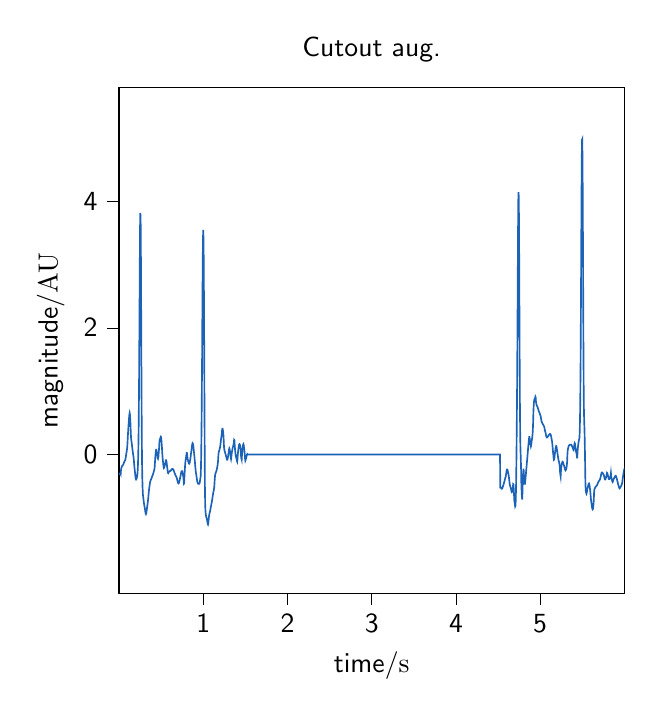
\begin{tikzpicture}
\pgfplotsset{
   every axis/.append style={
		font=\fontsize{10}{10}\sffamily},
	every non boxed x axis/.append style={
		x axis line style={->}
	},
	every non boxed y axis/.append style={
		y axis line style={->}
	},
	every non boxed z axis/.append style={
		z axis line style={->}
	}
}
\begin{axis}[
height=\figH,
tick align=outside,
tick pos=left,
width=\figW,
x grid style={white!69.0196078431373!black},
xlabel={time/$\si{\second}$},
xmin=0, xmax=6,
xtick style={color=black},
y grid style={white!69.0196078431373!black},
ylabel={magnitude/\si{AU}},
ymin=-2.19102610318908, ymax=5.78890501260757,
ytick style={color=black},
ytick = {0, 2, 4},
yticklabels = {0, 2, 4},
xtick = {1, 2, 3, 4, 5},
xticklabels = {1, 2, 3, 4, 5},
title = {Cutout aug.},
]
\addplot [semithick, tud1b]
table {%
0 -0.304270714521408
0.00333333341404796 -0.30953973531723
0.00666666682809591 -0.30953973531723
0.00999999977648258 -0.304270714521408
0.0133333336561918 -0.299001693725586
0.0166666675359011 -0.299001693725586
0.0199999995529652 -0.30953973531723
0.0233333334326744 -0.251580506563187
0.0266666673123837 -0.219966381788254
0.0299999993294477 -0.204159319400787
0.0333333350718021 -0.193621277809143
0.0366666652262211 -0.183083236217499
0.0399999991059303 -0.172545194625854
0.0433333329856396 -0.172545194625854
0.0466666668653488 -0.167276173830032
0.0500000007450581 -0.16200715303421
0.0533333346247673 -0.151469111442566
0.0566666685044765 -0.135662049055099
0.0599999986588955 -0.125124022364616
0.0633333325386047 -0.114585973322392
0.0666666701436043 -0.104047931730747
0.0700000002980232 -0.0987789109349251
0.0733333304524422 -0.0882408767938614
0.0766666680574417 -0.0724338069558144
0.0799999982118607 -0.0460887067019939
0.0833333358168602 -0.0197436045855284
0.0866666659712791 0.0118705164641142
0.0900000035762787 0.0382156185805798
0.0933333337306976 0.0645607188344002
0.0966666638851166 0.101443856954575
0.100000001490116 0.159403070807457
0.103333331644535 0.243707403540611
0.106666669249535 0.322742700576782
0.109999999403954 0.396509021520615
0.113333337008953 0.46500626206398
0.116666667163372 0.533503532409668
0.119999997317791 0.586193740367889
0.123333334922791 0.633614897727966
0.126666665077209 0.654690980911255
0.129999995231628 0.628345906734467
0.133333340287209 0.565117657184601
0.136666670441628 0.470275282859802
0.140000000596046 0.338549792766571
0.143333330750465 0.259514451026917
0.146666660904884 0.222631320357323
0.150000005960464 0.19101719558239
0.153333336114883 0.154134064912796
0.156666666269302 0.117250919342041
0.159999996423721 0.0803677812218666
0.16333332657814 0.0434846356511116
0.16666667163372 0.0118705164641142
0.170000001788139 -0.0144745847210288
0.173333331942558 -0.0513577274978161
0.176666662096977 -0.0935098901391029
0.180000007152557 -0.151469111442566
0.183333337306976 -0.204159319400787
0.186666667461395 -0.241042464971542
0.189999997615814 -0.28319463133812
0.193333327770233 -0.325346797704697
0.196666672825813 -0.362229913473129
0.200000002980232 -0.383305996656418
0.203333333134651 -0.393844038248062
0.20666666328907 -0.38857501745224
0.209999993443489 -0.378036975860596
0.213333338499069 -0.356960892677307
0.216666668653488 -0.330615818500519
0.219999998807907 -0.293732672929764
0.223333328962326 -0.225235402584076
0.226666674017906 -0.0935098901391029
0.230000004172325 0.0961748361587524
0.233333334326744 0.407047063112259
0.236666664481163 0.87072080373764
0.239999994635582 1.49246525764465
0.243333339691162 2.23012804985046
0.246666669845581 2.98886680603027
0.25 3.6053421497345
0.253333330154419 3.81610298156738
0.256666660308838 3.74760580062866
0.259999990463257 3.19962763786316
0.263333320617676 2.26174211502075
0.266666680574417 1.23955225944519
0.270000010728836 0.407047063112259
0.273333340883255 -0.109316952526569
0.276666671037674 -0.367498934268951
0.280000001192093 -0.525569558143616
0.283333331346512 -0.62041187286377
0.286666661500931 -0.662564039230347
0.28999999165535 -0.699447214603424
0.293333321809769 -0.736330389976501
0.296666651964188 -0.773213505744934
0.300000011920929 -0.799558639526367
0.303333342075348 -0.825903713703156
0.306666672229767 -0.846979796886444
0.310000002384186 -0.878593921661377
0.313333332538605 -0.91020804643631
0.316666662693024 -0.931284129619598
0.319999992847443 -0.941822171211243
0.323333323001862 -0.931284129619598
0.326666653156281 -0.90493905544281
0.330000013113022 -0.868055880069733
0.333333343267441 -0.8364417552948
0.33666667342186 -0.804827630519867
0.340000003576279 -0.773213505744934
0.343333333730698 -0.736330389976501
0.346666663885117 -0.694178223609924
0.349999994039536 -0.646757006645203
0.353333324193954 -0.599335789680481
0.356666654348373 -0.557183682918549
0.360000014305115 -0.520300507545471
0.363333344459534 -0.488686382770538
0.366666674613953 -0.457072257995605
0.370000004768372 -0.435996174812317
0.373333334922791 -0.414920121431351
0.376666665077209 -0.404382079839706
0.379999995231628 -0.393844038248062
0.383333325386047 -0.383305996656418
0.386666655540466 -0.372767955064774
0.389999985694885 -0.362229913473129
0.393333345651627 -0.346422851085663
0.396666675806046 -0.335884839296341
0.400000005960464 -0.325346797704697
0.403333336114883 -0.314808756113052
0.406666666269302 -0.299001693725586
0.409999996423721 -0.28319463133812
0.41333332657814 -0.267387568950653
0.416666656732559 -0.251580506563187
0.419999986886978 -0.23577344417572
0.423333346843719 -0.204159319400787
0.426666676998138 -0.130393028259277
0.430000007152557 -0.0618957690894604
0.433333337306976 -0.00393654452636838
0.436666667461395 0.0434846356511116
0.439999997615814 0.0750987604260445
0.443333327770233 0.0750987604260445
0.446666657924652 0.0487536564469337
0.449999988079071 0.0224085561931133
0.453333348035812 -0.00393654452636838
0.456666678190231 -0.0302816461771727
0.46000000834465 -0.0566267482936382
0.463333338499069 -0.0671647861599922
0.466666668653488 -0.0513577274978161
0.469999998807907 -0.00393654452636838
0.473333328962326 0.0540226772427559
0.476666659116745 0.117250919342041
0.479999989271164 0.201555237174034
0.483333319425583 0.233169361948967
0.486666679382324 0.243707403540611
0.490000009536743 0.254245430231094
0.493333339691162 0.270052492618561
0.496666669845581 0.280590534210205
0.5 0.275321513414383
0.503333330154419 0.227900341153145
0.506666660308838 0.164672091603279
0.509999990463257 0.106712877750397
0.513333320617676 0.0276775769889355
0.516666650772095 -0.0355506651103497
0.519999980926514 -0.0829718485474586
0.523333311080933 -0.125124022364616
0.526666641235352 -0.167276173830032
0.529999971389771 -0.198890298604965
0.533333361148834 -0.214697360992432
0.536666691303253 -0.209428340196609
0.540000021457672 -0.193621277809143
0.543333351612091 -0.172545194625854
0.54666668176651 -0.156738132238388
0.550000011920929 -0.135662049055099
0.553333342075348 -0.109316952526569
0.556666672229767 -0.0882408767938614
0.560000002384186 -0.0882408767938614
0.563333332538605 -0.109316952526569
0.566666662693024 -0.140931069850922
0.569999992847443 -0.177814215421677
0.573333323001862 -0.209428340196609
0.576666653156281 -0.251580506563187
0.579999983310699 -0.288463652133942
0.583333313465118 -0.293732672929764
0.586666643619537 -0.28319463133812
0.589999973773956 -0.277925610542297
0.593333303928375 -0.272656589746475
0.596666693687439 -0.272656589746475
0.600000023841858 -0.267387568950653
0.603333353996277 -0.262118548154831
0.606666684150696 -0.262118548154831
0.610000014305115 -0.256849527359009
0.613333344459534 -0.256849527359009
0.616666674613953 -0.251580506563187
0.620000004768372 -0.246311485767365
0.623333334922791 -0.23577344417572
0.626666665077209 -0.23577344417572
0.629999995231628 -0.230504423379898
0.633333325386047 -0.23577344417572
0.636666655540466 -0.23577344417572
0.639999985694885 -0.230504423379898
0.643333315849304 -0.23577344417572
0.646666646003723 -0.241042464971542
0.649999976158142 -0.251580506563187
0.653333306312561 -0.267387568950653
0.656666696071625 -0.277925610542297
0.660000026226044 -0.293732672929764
0.663333356380463 -0.304270714521408
0.666666686534882 -0.314808756113052
0.670000016689301 -0.325346797704697
0.673333346843719 -0.335884839296341
0.676666676998138 -0.341153830289841
0.680000007152557 -0.351691871881485
0.683333337306976 -0.362229913473129
0.686666667461395 -0.372767955064774
0.689999997615814 -0.393844038248062
0.693333327770233 -0.409651100635529
0.696666657924652 -0.430727183818817
0.699999988079071 -0.446534216403961
0.70333331823349 -0.451803237199783
0.706666648387909 -0.457072257995605
0.709999978542328 -0.451803237199783
0.713333308696747 -0.441265195608139
0.716666638851166 -0.425458163022995
0.720000028610229 -0.404382079839706
0.723333358764648 -0.383305996656418
0.726666688919067 -0.362229913473129
0.730000019073486 -0.341153830289841
0.733333349227905 -0.320077776908875
0.736666679382324 -0.293732672929764
0.740000009536743 -0.277925610542297
0.743333339691162 -0.262118548154831
0.746666669845581 -0.262118548154831
0.75 -0.262118548154831
0.753333330154419 -0.277925610542297
0.756666660308838 -0.299001693725586
0.759999990463257 -0.325346797704697
0.763333320617676 -0.351691871881485
0.766666650772095 -0.393844038248062
0.769999980926514 -0.462341278791428
0.773333311080933 -0.457072257995605
0.776666641235352 -0.356960892677307
0.779999971389771 -0.272656589746475
0.783333361148834 -0.198890298604965
0.786666691303253 -0.140931069850922
0.790000021457672 -0.0987789109349251
0.793333351612091 -0.0724338069558144
0.79666668176651 -0.0408196859061718
0.800000011920929 -0.00393654452636838
0.803333342075348 0.0224085561931133
0.806666672229767 0.0224085561931133
0.810000002384186 -0.0144745847210288
0.813333332538605 -0.0566267482936382
0.816666662693024 -0.0777028277516365
0.819999992847443 -0.0935098901391029
0.823333323001862 -0.114585973322392
0.826666653156281 -0.130393028259277
0.829999983310699 -0.140931069850922
0.833333313465118 -0.146200090646744
0.836666643619537 -0.140931069850922
0.839999973773956 -0.125124022364616
0.843333303928375 -0.0987789109349251
0.846666693687439 -0.0724338069558144
0.850000023841858 -0.0408196859061718
0.853333353996277 -0.00393654452636838
0.856666684150696 0.0276775769889355
0.860000014305115 0.0645607188344002
0.863333344459534 0.101443856954575
0.866666674613953 0.13832700252533
0.870000004768372 0.164672091603279
0.873333334922791 0.180479153990746
0.876666665077209 0.175210133194923
0.879999995231628 0.154134064912796
0.883333325386047 0.122519932687283
0.886666655540466 0.0803677812218666
0.889999985694885 0.0382156185805798
0.893333315849304 -0.00393654452636838
0.896666646003723 -0.0513577274978161
0.899999976158142 -0.0987789109349251
0.903333306312561 -0.151469111442566
0.906666696071625 -0.204159319400787
0.910000026226044 -0.251580506563187
0.913333356380463 -0.288463652133942
0.916666686534882 -0.314808756113052
0.920000016689301 -0.341153830289841
0.923333346843719 -0.372767955064774
0.926666676998138 -0.404382079839706
0.930000007152557 -0.430727183818817
0.933333337306976 -0.446534216403961
0.936666667461395 -0.457072257995605
0.939999997615814 -0.462341278791428
0.943333327770233 -0.462341278791428
0.946666657924652 -0.462341278791428
0.949999988079071 -0.462341278791428
0.95333331823349 -0.462341278791428
0.956666648387909 -0.451803237199783
0.959999978542328 -0.430727183818817
0.963333308696747 -0.399113059043884
0.966666638851166 -0.367498934268951
0.970000028610229 -0.341153830289841
0.973333358764648 -0.198890298604965
0.976666688919067 0.0698297396302223
0.980000019073486 0.449199199676514
0.983333349227905 0.94975608587265
0.986666679382324 1.57150053977966
0.990000009536743 2.27228021621704
0.993333339691162 2.93617653846741
0.996666669845581 3.38931226730347
1 3.54738306999207
1.00333333015442 3.4051194190979
1.00666666030884 2.96252179145813
1.00999999046326 2.14582371711731
1.01333332061768 1.19740009307861
1.01666665077209 0.248976424336433
1.01999998092651 -0.509762465953827
1.02333331108093 -0.804827630519867
1.02666664123535 -0.894401013851166
1.02999997138977 -0.941822171211243
1.03333330154419 -0.968167245388031
1.03666663169861 -0.98924332857132
1.03999996185303 -1.00505042076111
1.04333329200745 -1.02085745334625
1.04666662216187 -1.04193353652954
1.04999995231628 -1.06827867031097
1.0533332824707 -1.09462380409241
1.05666661262512 -1.10516178607941
1.05999994277954 -1.08935475349426
1.06333339214325 -1.04720258712769
1.06666672229767 -0.994512379169464
1.07000005245209 -0.962898254394531
1.07333338260651 -0.941822171211243
1.07666671276093 -0.920746088027954
1.08000004291534 -0.90493905544281
1.08333337306976 -0.878593921661377
1.08666670322418 -0.857517838478088
1.0900000333786 -0.8311727643013
1.09333336353302 -0.810096681118011
1.09666669368744 -0.783751547336578
1.10000002384186 -0.76267546415329
1.10333335399628 -0.736330389976501
1.1066666841507 -0.709985256195068
1.11000001430511 -0.678371131420135
1.11333334445953 -0.652025997638702
1.11666667461395 -0.62041187286377
1.12000000476837 -0.599335789680481
1.12333333492279 -0.578259706497192
1.12666666507721 -0.551914632320404
1.12999999523163 -0.525569558143616
1.13333332538605 -0.46761029958725
1.13666665554047 -0.38857501745224
1.13999998569489 -0.335884839296341
1.1433333158493 -0.30953973531723
1.14666664600372 -0.293732672929764
1.14999997615814 -0.28319463133812
1.15333330631256 -0.272656589746475
1.15666663646698 -0.256849527359009
1.1599999666214 -0.241042464971542
1.16333329677582 -0.219966381788254
1.16666662693024 -0.198890298604965
1.16999995708466 -0.172545194625854
1.17333328723907 -0.135662049055099
1.17666661739349 -0.0882408767938614
1.17999994754791 -0.0144745847210288
1.18333327770233 0.0329465977847576
1.18666660785675 0.0487536564469337
1.19000005722046 0.0645607188344002
1.19333338737488 0.0750987604260445
1.1966667175293 0.0961748361587524
1.20000004768372 0.117250919342041
1.20333337783813 0.143596023321152
1.20666670799255 0.180479153990746
1.21000003814697 0.222631320357323
1.21333336830139 0.259514451026917
1.21666669845581 0.291128575801849
1.22000002861023 0.333280742168427
1.22333335876465 0.380701959133148
1.22666668891907 0.407047063112259
1.23000001907349 0.407047063112259
1.23333334922791 0.38597097992897
1.23666667938232 0.349087834358215
1.24000000953674 0.306935638189316
1.24333333969116 0.222631320357323
1.24666666984558 0.117250919342041
1.25 0.0803677812218666
1.25333333015442 0.059291698038578
1.25666666030884 0.0434846356511116
1.25999999046326 0.0276775769889355
1.26333332061768 0.0118705164641142
1.26666665077209 -0.00393654452636838
1.26999998092651 -0.0197436045855284
1.27333331108093 -0.0355506651103497
1.27666664123535 -0.0566267482936382
1.27999997138977 -0.0777028277516365
1.28333330154419 -0.0829718485474586
1.28666663169861 -0.0829718485474586
1.28999996185303 -0.0671647861599922
1.29333329200745 -0.0408196859061718
1.29666662216187 -0.00920556485652924
1.29999995231628 0.0118705164641142
1.3033332824707 0.0487536564469337
1.30666661262512 0.0803677812218666
1.30999994277954 0.0961748361587524
1.31333339214325 0.0856367945671082
1.31666672229767 0.059291698038578
1.32000005245209 0.0276775769889355
1.32333338260651 -0.00393654452636838
1.32666671276093 -0.0513577274978161
1.33000004291534 -0.0724338069558144
1.33333337306976 -0.0460887067019939
1.33666670322418 0.00133247557096183
1.3400000333786 0.0329465977847576
1.34333336353302 0.059291698038578
1.34666669368744 0.0856367945671082
1.35000002384186 0.106712877750397
1.35333335399628 0.122519932687283
1.3566666841507 0.13832700252533
1.36000001430511 0.159403070807457
1.36333334445953 0.185748174786568
1.36666667461395 0.233169361948967
1.37000000476837 0.227900341153145
1.37333333492279 0.154134064912796
1.37666666507721 0.0961748361587524
1.37999999523163 0.0487536564469337
1.38333332538605 0.00660149566829205
1.38666665554047 -0.0197436045855284
1.38999998569489 -0.0408196859061718
1.3933333158493 -0.0566267482936382
1.39666664600372 -0.0777028277516365
1.39999997615814 -0.104047931730747
1.40333330631256 -0.114585973322392
1.40666663646698 -0.0777028277516365
1.4099999666214 -0.00393654452636838
1.41333329677582 0.0382156185805798
1.41666662693024 0.0750987604260445
1.41999995708466 0.111981898546219
1.42333328723907 0.143596023321152
1.42666661739349 0.159403070807457
1.42999994754791 0.164672091603279
1.43333327770233 0.159403070807457
1.43666660785675 0.143596023321152
1.44000005722046 0.122519932687283
1.44333338737488 0.0909058153629303
1.4466667175293 0.0276775769889355
1.45000004768372 -0.0408196859061718
1.45333337783813 -0.0671647861599922
1.45666670799255 -0.0829718485474586
1.46000003814697 -0.00920556485652924
1.46333336830139 0.0540226772427559
1.46666669845581 0.0909058153629303
1.47000002861023 0.127788960933685
1.47333335876465 0.154134064912796
1.47666668891907 0.164672091603279
1.48000001907349 0.154134064912796
1.48333334922791 0.122519932687283
1.48666667938232 0.0856367945671082
1.49000000953674 0.0434846356511116
1.49333333969116 0.00133247557096183
1.49666666984558 -0.0671647861599922
1.5 -0.0987789109349251
1.50333333015442 -0.0882408767938614
1.50666666030884 -0.0671647861599922
1.50999999046326 -0.0513577274978161
1.51333332061768 -0.0355506651103497
1.51666665077209 -0.0144745847210288
1.51999998092651 0.00133247557096183
1.52333331108093 0.00660149566829205
1.52666664123535 0
1.52999997138977 0
1.53333330154419 0
1.53666663169861 0
1.53999996185303 0
1.54333329200745 0
1.54666662216187 0
1.54999995231628 0
1.5533332824707 0
1.55666661262512 0
1.55999994277954 0
1.56333339214325 0
1.56666672229767 0
1.57000005245209 0
1.57333338260651 0
1.57666671276093 0
1.58000004291534 0
1.58333337306976 0
1.58666670322418 0
1.5900000333786 0
1.59333336353302 0
1.59666669368744 0
1.60000002384186 0
1.60333335399628 0
1.6066666841507 0
1.61000001430511 0
1.61333334445953 0
1.61666667461395 0
1.62000000476837 0
1.62333333492279 0
1.62666666507721 0
1.62999999523163 0
1.63333332538605 0
1.63666665554047 0
1.63999998569489 0
1.6433333158493 0
1.64666664600372 0
1.64999997615814 0
1.65333330631256 0
1.65666663646698 0
1.6599999666214 0
1.66333329677582 0
1.66666662693024 0
1.66999995708466 0
1.67333328723907 0
1.67666661739349 0
1.67999994754791 0
1.68333327770233 0
1.68666660785675 0
1.69000005722046 0
1.69333338737488 0
1.6966667175293 0
1.70000004768372 0
1.70333337783813 0
1.70666670799255 0
1.71000003814697 0
1.71333336830139 0
1.71666669845581 0
1.72000002861023 0
1.72333335876465 0
1.72666668891907 0
1.73000001907349 0
1.73333334922791 0
1.73666667938232 0
1.74000000953674 0
1.74333333969116 0
1.74666666984558 0
1.75 0
1.75333333015442 0
1.75666666030884 0
1.75999999046326 0
1.76333332061768 0
1.76666665077209 0
1.76999998092651 0
1.77333331108093 0
1.77666664123535 0
1.77999997138977 0
1.78333330154419 0
1.78666663169861 0
1.78999996185303 0
1.79333329200745 0
1.79666662216187 0
1.79999995231628 0
1.8033332824707 0
1.80666661262512 0
1.80999994277954 0
1.81333339214325 0
1.81666672229767 0
1.82000005245209 0
1.82333338260651 0
1.82666671276093 0
1.83000004291534 0
1.83333337306976 0
1.83666670322418 0
1.8400000333786 0
1.84333336353302 0
1.84666669368744 0
1.85000002384186 0
1.85333335399628 0
1.8566666841507 0
1.86000001430511 0
1.86333334445953 0
1.86666667461395 0
1.87000000476837 0
1.87333333492279 0
1.87666666507721 0
1.87999999523163 0
1.88333332538605 0
1.88666665554047 0
1.88999998569489 0
1.8933333158493 0
1.89666664600372 0
1.89999997615814 0
1.90333330631256 0
1.90666663646698 0
1.9099999666214 0
1.91333329677582 0
1.91666662693024 0
1.91999995708466 0
1.92333328723907 0
1.92666661739349 0
1.92999994754791 0
1.93333327770233 0
1.93666660785675 0
1.94000005722046 0
1.94333338737488 0
1.9466667175293 0
1.95000004768372 0
1.95333337783813 0
1.95666670799255 0
1.96000003814697 0
1.96333336830139 0
1.96666669845581 0
1.97000002861023 0
1.97333335876465 0
1.97666668891907 0
1.98000001907349 0
1.98333334922791 0
1.98666667938232 0
1.99000000953674 0
1.99333333969116 0
1.99666666984558 0
2 0
2.00333333015442 0
2.00666666030884 0
2.00999999046326 0
2.01333332061768 0
2.01666665077209 0
2.01999998092651 0
2.02333331108093 0
2.02666664123535 0
2.02999997138977 0
2.03333330154419 0
2.03666663169861 0
2.03999996185303 0
2.04333329200745 0
2.04666662216187 0
2.04999995231628 0
2.0533332824707 0
2.05666661262512 0
2.05999994277954 0
2.06333327293396 0
2.06666660308838 0
2.0699999332428 0
2.07333326339722 0
2.07666659355164 0
2.07999992370605 0
2.08333325386047 0
2.08666658401489 0
2.08999991416931 0
2.09333324432373 0
2.09666657447815 0
2.09999990463257 0
2.10333323478699 0
2.10666656494141 0
2.10999989509583 0
2.11333322525024 0
2.11666655540466 0
2.11999988555908 0
2.1233332157135 0
2.1266667842865 0
2.13000011444092 0
2.13333344459534 0
2.13666677474976 0
2.14000010490417 0
2.14333343505859 0
2.14666676521301 0
2.15000009536743 0
2.15333342552185 0
2.15666675567627 0
2.16000008583069 0
2.16333341598511 0
2.16666674613953 0
2.17000007629395 0
2.17333340644836 0
2.17666673660278 0
2.1800000667572 0
2.18333339691162 0
2.18666672706604 0
2.19000005722046 0
2.19333338737488 0
2.1966667175293 0
2.20000004768372 0
2.20333337783813 0
2.20666670799255 0
2.21000003814697 0
2.21333336830139 0
2.21666669845581 0
2.22000002861023 0
2.22333335876465 0
2.22666668891907 0
2.23000001907349 0
2.23333334922791 0
2.23666667938232 0
2.24000000953674 0
2.24333333969116 0
2.24666666984558 0
2.25 0
2.25333333015442 0
2.25666666030884 0
2.25999999046326 0
2.26333332061768 0
2.26666665077209 0
2.26999998092651 0
2.27333331108093 0
2.27666664123535 0
2.27999997138977 0
2.28333330154419 0
2.28666663169861 0
2.28999996185303 0
2.29333329200745 0
2.29666662216187 0
2.29999995231628 0
2.3033332824707 0
2.30666661262512 0
2.30999994277954 0
2.31333327293396 0
2.31666660308838 0
2.3199999332428 0
2.32333326339722 0
2.32666659355164 0
2.32999992370605 0
2.33333325386047 0
2.33666658401489 0
2.33999991416931 0
2.34333324432373 0
2.34666657447815 0
2.34999990463257 0
2.35333323478699 0
2.35666656494141 0
2.35999989509583 0
2.36333322525024 0
2.36666655540466 0
2.36999988555908 0
2.3733332157135 0
2.3766667842865 0
2.38000011444092 0
2.38333344459534 0
2.38666677474976 0
2.39000010490417 0
2.39333343505859 0
2.39666676521301 0
2.40000009536743 0
2.40333342552185 0
2.40666675567627 0
2.41000008583069 0
2.41333341598511 0
2.41666674613953 0
2.42000007629395 0
2.42333340644836 0
2.42666673660278 0
2.4300000667572 0
2.43333339691162 0
2.43666672706604 0
2.44000005722046 0
2.44333338737488 0
2.4466667175293 0
2.45000004768372 0
2.45333337783813 0
2.45666670799255 0
2.46000003814697 0
2.46333336830139 0
2.46666669845581 0
2.47000002861023 0
2.47333335876465 0
2.47666668891907 0
2.48000001907349 0
2.48333334922791 0
2.48666667938232 0
2.49000000953674 0
2.49333333969116 0
2.49666666984558 0
2.5 0
2.50333333015442 0
2.50666666030884 0
2.50999999046326 0
2.51333332061768 0
2.51666665077209 0
2.51999998092651 0
2.52333331108093 0
2.52666664123535 0
2.52999997138977 0
2.53333330154419 0
2.53666663169861 0
2.53999996185303 0
2.54333329200745 0
2.54666662216187 0
2.54999995231628 0
2.5533332824707 0
2.55666661262512 0
2.55999994277954 0
2.56333327293396 0
2.56666660308838 0
2.5699999332428 0
2.57333326339722 0
2.57666659355164 0
2.57999992370605 0
2.58333325386047 0
2.58666658401489 0
2.58999991416931 0
2.59333324432373 0
2.59666657447815 0
2.59999990463257 0
2.60333323478699 0
2.60666656494141 0
2.60999989509583 0
2.61333322525024 0
2.61666655540466 0
2.61999988555908 0
2.6233332157135 0
2.6266667842865 0
2.63000011444092 0
2.63333344459534 0
2.63666677474976 0
2.64000010490417 0
2.64333343505859 0
2.64666676521301 0
2.65000009536743 0
2.65333342552185 0
2.65666675567627 0
2.66000008583069 0
2.66333341598511 0
2.66666674613953 0
2.67000007629395 0
2.67333340644836 0
2.67666673660278 0
2.6800000667572 0
2.68333339691162 0
2.68666672706604 0
2.69000005722046 0
2.69333338737488 0
2.6966667175293 0
2.70000004768372 0
2.70333337783813 0
2.70666670799255 0
2.71000003814697 0
2.71333336830139 0
2.71666669845581 0
2.72000002861023 0
2.72333335876465 0
2.72666668891907 0
2.73000001907349 0
2.73333334922791 0
2.73666667938232 0
2.74000000953674 0
2.74333333969116 0
2.74666666984558 0
2.75 0
2.75333333015442 0
2.75666666030884 0
2.75999999046326 0
2.76333332061768 0
2.76666665077209 0
2.76999998092651 0
2.77333331108093 0
2.77666664123535 0
2.77999997138977 0
2.78333330154419 0
2.78666663169861 0
2.78999996185303 0
2.79333329200745 0
2.79666662216187 0
2.79999995231628 0
2.8033332824707 0
2.80666661262512 0
2.80999994277954 0
2.81333327293396 0
2.81666660308838 0
2.8199999332428 0
2.82333326339722 0
2.82666659355164 0
2.82999992370605 0
2.83333325386047 0
2.83666658401489 0
2.83999991416931 0
2.84333324432373 0
2.84666657447815 0
2.84999990463257 0
2.85333323478699 0
2.85666656494141 0
2.85999989509583 0
2.86333322525024 0
2.86666655540466 0
2.86999988555908 0
2.8733332157135 0
2.8766667842865 0
2.88000011444092 0
2.88333344459534 0
2.88666677474976 0
2.89000010490417 0
2.89333343505859 0
2.89666676521301 0
2.90000009536743 0
2.90333342552185 0
2.90666675567627 0
2.91000008583069 0
2.91333341598511 0
2.91666674613953 0
2.92000007629395 0
2.92333340644836 0
2.92666673660278 0
2.9300000667572 0
2.93333339691162 0
2.93666672706604 0
2.94000005722046 0
2.94333338737488 0
2.9466667175293 0
2.95000004768372 0
2.95333337783813 0
2.95666670799255 0
2.96000003814697 0
2.96333336830139 0
2.96666669845581 0
2.97000002861023 0
2.97333335876465 0
2.97666668891907 0
2.98000001907349 0
2.98333334922791 0
2.98666667938232 0
2.99000000953674 0
2.99333333969116 0
2.99666666984558 0
3 0
3.00333333015442 0
3.00666666030884 0
3.00999999046326 0
3.01333332061768 0
3.01666665077209 0
3.01999998092651 0
3.02333331108093 0
3.02666664123535 0
3.02999997138977 0
3.03333330154419 0
3.03666663169861 0
3.03999996185303 0
3.04333329200745 0
3.04666662216187 0
3.04999995231628 0
3.0533332824707 0
3.05666661262512 0
3.05999994277954 0
3.06333327293396 0
3.06666660308838 0
3.0699999332428 0
3.07333326339722 0
3.07666659355164 0
3.07999992370605 0
3.08333325386047 0
3.08666658401489 0
3.08999991416931 0
3.09333324432373 0
3.09666657447815 0
3.09999990463257 0
3.10333323478699 0
3.10666656494141 0
3.10999989509583 0
3.11333322525024 0
3.11666655540466 0
3.11999988555908 0
3.1233332157135 0
3.1266667842865 0
3.13000011444092 0
3.13333344459534 0
3.13666677474976 0
3.14000010490417 0
3.14333343505859 0
3.14666676521301 0
3.15000009536743 0
3.15333342552185 0
3.15666675567627 0
3.16000008583069 0
3.16333341598511 0
3.16666674613953 0
3.17000007629395 0
3.17333340644836 0
3.17666673660278 0
3.1800000667572 0
3.18333339691162 0
3.18666672706604 0
3.19000005722046 0
3.19333338737488 0
3.1966667175293 0
3.20000004768372 0
3.20333337783813 0
3.20666670799255 0
3.21000003814697 0
3.21333336830139 0
3.21666669845581 0
3.22000002861023 0
3.22333335876465 0
3.22666668891907 0
3.23000001907349 0
3.23333334922791 0
3.23666667938232 0
3.24000000953674 0
3.24333333969116 0
3.24666666984558 0
3.25 0
3.25333333015442 0
3.25666666030884 0
3.25999999046326 0
3.26333332061768 0
3.26666665077209 0
3.26999998092651 0
3.27333331108093 0
3.27666664123535 0
3.27999997138977 0
3.28333330154419 0
3.28666663169861 0
3.28999996185303 0
3.29333329200745 0
3.29666662216187 0
3.29999995231628 0
3.3033332824707 0
3.30666661262512 0
3.30999994277954 0
3.31333327293396 0
3.31666660308838 0
3.3199999332428 0
3.32333326339722 0
3.32666659355164 0
3.32999992370605 0
3.33333325386047 0
3.33666658401489 0
3.33999991416931 0
3.34333324432373 0
3.34666657447815 0
3.34999990463257 0
3.35333323478699 0
3.35666656494141 0
3.35999989509583 0
3.36333322525024 0
3.36666655540466 0
3.36999988555908 0
3.3733332157135 0
3.3766667842865 0
3.38000011444092 0
3.38333344459534 0
3.38666677474976 0
3.39000010490417 0
3.39333343505859 0
3.39666676521301 0
3.40000009536743 0
3.40333342552185 0
3.40666675567627 0
3.41000008583069 0
3.41333341598511 0
3.41666674613953 0
3.42000007629395 0
3.42333340644836 0
3.42666673660278 0
3.4300000667572 0
3.43333339691162 0
3.43666672706604 0
3.44000005722046 0
3.44333338737488 0
3.4466667175293 0
3.45000004768372 0
3.45333337783813 0
3.45666670799255 0
3.46000003814697 0
3.46333336830139 0
3.46666669845581 0
3.47000002861023 0
3.47333335876465 0
3.47666668891907 0
3.48000001907349 0
3.48333334922791 0
3.48666667938232 0
3.49000000953674 0
3.49333333969116 0
3.49666666984558 0
3.5 0
3.50333333015442 0
3.50666666030884 0
3.50999999046326 0
3.51333332061768 0
3.51666665077209 0
3.51999998092651 0
3.52333331108093 0
3.52666664123535 0
3.52999997138977 0
3.53333330154419 0
3.53666663169861 0
3.53999996185303 0
3.54333329200745 0
3.54666662216187 0
3.54999995231628 0
3.5533332824707 0
3.55666661262512 0
3.55999994277954 0
3.56333327293396 0
3.56666660308838 0
3.5699999332428 0
3.57333326339722 0
3.57666659355164 0
3.57999992370605 0
3.58333325386047 0
3.58666658401489 0
3.58999991416931 0
3.59333324432373 0
3.59666657447815 0
3.59999990463257 0
3.60333323478699 0
3.60666656494141 0
3.60999989509583 0
3.61333322525024 0
3.61666655540466 0
3.61999988555908 0
3.6233332157135 0
3.6266667842865 0
3.63000011444092 0
3.63333344459534 0
3.63666677474976 0
3.64000010490417 0
3.64333343505859 0
3.64666676521301 0
3.65000009536743 0
3.65333342552185 0
3.65666675567627 0
3.66000008583069 0
3.66333341598511 0
3.66666674613953 0
3.67000007629395 0
3.67333340644836 0
3.67666673660278 0
3.6800000667572 0
3.68333339691162 0
3.68666672706604 0
3.69000005722046 0
3.69333338737488 0
3.6966667175293 0
3.70000004768372 0
3.70333337783813 0
3.70666670799255 0
3.71000003814697 0
3.71333336830139 0
3.71666669845581 0
3.72000002861023 0
3.72333335876465 0
3.72666668891907 0
3.73000001907349 0
3.73333334922791 0
3.73666667938232 0
3.74000000953674 0
3.74333333969116 0
3.74666666984558 0
3.75 0
3.75333333015442 0
3.75666666030884 0
3.75999999046326 0
3.76333332061768 0
3.76666665077209 0
3.76999998092651 0
3.77333331108093 0
3.77666664123535 0
3.77999997138977 0
3.78333330154419 0
3.78666663169861 0
3.78999996185303 0
3.79333329200745 0
3.79666662216187 0
3.79999995231628 0
3.8033332824707 0
3.80666661262512 0
3.80999994277954 0
3.81333327293396 0
3.81666660308838 0
3.8199999332428 0
3.82333326339722 0
3.82666659355164 0
3.82999992370605 0
3.83333325386047 0
3.83666658401489 0
3.83999991416931 0
3.84333324432373 0
3.84666657447815 0
3.84999990463257 0
3.85333323478699 0
3.85666656494141 0
3.85999989509583 0
3.86333322525024 0
3.86666655540466 0
3.86999988555908 0
3.8733332157135 0
3.8766667842865 0
3.88000011444092 0
3.88333344459534 0
3.88666677474976 0
3.89000010490417 0
3.89333343505859 0
3.89666676521301 0
3.90000009536743 0
3.90333342552185 0
3.90666675567627 0
3.91000008583069 0
3.91333341598511 0
3.91666674613953 0
3.92000007629395 0
3.92333340644836 0
3.92666673660278 0
3.9300000667572 0
3.93333339691162 0
3.93666672706604 0
3.94000005722046 0
3.94333338737488 0
3.9466667175293 0
3.95000004768372 0
3.95333337783813 0
3.95666670799255 0
3.96000003814697 0
3.96333336830139 0
3.96666669845581 0
3.97000002861023 0
3.97333335876465 0
3.97666668891907 0
3.98000001907349 0
3.98333334922791 0
3.98666667938232 0
3.99000000953674 0
3.99333333969116 0
3.99666666984558 0
4 0
4.003333568573 0
4.00666666030884 0
4.01000022888184 0
4.01333332061768 0
4.01666688919067 0
4.01999998092651 0
4.02333354949951 0
4.02666664123535 0
4.03000020980835 0
4.03333330154419 0
4.03666687011719 0
4.03999996185303 0
4.04333353042603 0
4.04666662216187 0
4.05000019073486 0
4.0533332824707 0
4.0566668510437 0
4.05999994277954 0
4.06333351135254 0
4.06666660308838 0
4.07000017166138 0
4.07333326339722 0
4.07666683197021 0
4.07999992370605 0
4.08333349227905 0
4.08666658401489 0
4.09000015258789 0
4.09333324432373 0
4.09666681289673 0
4.09999990463257 0
4.10333347320557 0
4.10666656494141 0
4.1100001335144 0
4.11333322525024 0
4.11666679382324 0
4.11999988555908 0
4.12333345413208 0
4.12666654586792 0
4.13000011444092 0
4.13333320617676 0
4.13666677474976 0
4.1399998664856 0
4.14333343505859 0
4.14666652679443 0
4.15000009536743 0
4.15333318710327 0
4.15666675567627 0
4.15999984741211 0
4.16333341598511 0
4.16666650772095 0
4.17000007629395 0
4.17333316802979 0
4.17666673660278 0
4.17999982833862 0
4.18333339691162 0
4.18666648864746 0
4.19000005722046 0
4.1933331489563 0
4.1966667175293 0
4.19999980926514 0
4.20333337783813 0
4.20666646957397 0
4.21000003814697 0
4.21333312988281 0
4.21666669845581 0
4.21999979019165 0
4.22333335876465 0
4.22666645050049 0
4.23000001907349 0
4.23333311080933 0
4.23666667938232 0
4.23999977111816 0
4.24333333969116 0
4.246666431427 0
4.25 0
4.253333568573 0
4.25666666030884 0
4.26000022888184 0
4.26333332061768 0
4.26666688919067 0
4.26999998092651 0
4.27333354949951 0
4.27666664123535 0
4.28000020980835 0
4.28333330154419 0
4.28666687011719 0
4.28999996185303 0
4.29333353042603 0
4.29666662216187 0
4.30000019073486 0
4.3033332824707 0
4.3066668510437 0
4.30999994277954 0
4.31333351135254 0
4.31666660308838 0
4.32000017166138 0
4.32333326339722 0
4.32666683197021 0
4.32999992370605 0
4.33333349227905 0
4.33666658401489 0
4.34000015258789 0
4.34333324432373 0
4.34666681289673 0
4.34999990463257 0
4.35333347320557 0
4.35666656494141 0
4.3600001335144 0
4.36333322525024 0
4.36666679382324 0
4.36999988555908 0
4.37333345413208 0
4.37666654586792 0
4.38000011444092 0
4.38333320617676 0
4.38666677474976 0
4.3899998664856 0
4.39333343505859 0
4.39666652679443 0
4.40000009536743 0
4.40333318710327 0
4.40666675567627 0
4.40999984741211 0
4.41333341598511 0
4.41666650772095 0
4.42000007629395 0
4.42333316802979 0
4.42666673660278 0
4.42999982833862 0
4.43333339691162 0
4.43666648864746 0
4.44000005722046 0
4.4433331489563 0
4.4466667175293 0
4.44999980926514 0
4.45333337783813 0
4.45666646957397 0
4.46000003814697 0
4.46333312988281 0
4.46666669845581 0
4.46999979019165 0
4.47333335876465 0
4.47666645050049 0
4.48000001907349 0
4.48333311080933 0
4.48666667938232 0
4.48999977111816 0
4.49333333969116 0
4.496666431427 0
4.5 0
4.503333568573 0
4.50666666030884 0
4.51000022888184 0
4.51333332061768 0
4.51666688919067 0
4.51999998092651 0
4.52333354949951 0
4.52666664123535 -0.520300507545471
4.53000020980835 -0.520300507545471
4.53333330154419 -0.525569558143616
4.53666687011719 -0.525569558143616
4.53999996185303 -0.53610759973526
4.54333353042603 -0.54137659072876
4.54666662216187 -0.54137659072876
4.55000019073486 -0.53610759973526
4.5533332824707 -0.525569558143616
4.5566668510437 -0.509762465953827
4.55999994277954 -0.49395540356636
4.56333351135254 -0.483417361974716
4.56666660308838 -0.46761029958725
4.57000017166138 -0.451803237199783
4.57333326339722 -0.435996174812317
4.57666683197021 -0.420189142227173
4.57999992370605 -0.399113059043884
4.58333349227905 -0.383305996656418
4.58666658401489 -0.367498934268951
4.59000015258789 -0.356960892677307
4.59333324432373 -0.330615818500519
4.59666681289673 -0.304270714521408
4.59999990463257 -0.272656589746475
4.60333347320557 -0.246311485767365
4.60666656494141 -0.23577344417572
4.6100001335144 -0.23577344417572
4.61333322525024 -0.246311485767365
4.61666679382324 -0.267387568950653
4.61999988555908 -0.288463652133942
4.62333345413208 -0.30953973531723
4.62666654586792 -0.335884839296341
4.63000011444092 -0.367498934268951
4.63333320617676 -0.409651100635529
4.63666677474976 -0.446534216403961
4.6399998664856 -0.478148341178894
4.64333343505859 -0.49395540356636
4.64666652679443 -0.509762465953827
4.65000009536743 -0.525569558143616
4.65333318710327 -0.54137659072876
4.65666675567627 -0.562452673912048
4.65999984741211 -0.583528757095337
4.66333341598511 -0.594066798686981
4.66666650772095 -0.588797748088837
4.67000007629395 -0.567721724510193
4.67333316802979 -0.54137659072876
4.67666673660278 -0.509762465953827
4.67999982833862 -0.46761029958725
4.68333339691162 -0.472879320383072
4.68666648864746 -0.551914632320404
4.69000005722046 -0.641487956047058
4.6933331489563 -0.725792348384857
4.6966667175293 -0.75740647315979
4.69999980926514 -0.789020597934723
4.70333337783813 -0.820634722709656
4.70666646957397 -0.810096681118011
4.71000003814697 -0.736330389976501
4.71333312988281 -0.551914632320404
4.71666669845581 -0.256849527359009
4.71999979019165 0.117250919342041
4.72333335876465 0.575655698776245
4.72666645050049 1.1394407749176
4.73000001907349 1.82968258857727
4.73333311080933 2.60949754714966
4.73666667938232 3.37877440452576
4.73999977111816 3.98998069763184
4.74333333969116 4.14278221130371
4.746666431427 4.04793977737427
4.75 3.42092657089233
4.753333568573 2.49357914924622
4.75666666030884 1.53461742401123
4.76000022888184 0.749533295631409
4.76333332061768 0.270052492618561
4.76666688919067 0.059291698038578
4.76999998092651 -0.0513577274978161
4.77333354949951 -0.214697360992432
4.77666664123535 -0.462341278791428
4.78000020980835 -0.578259706497192
4.78333330154419 -0.662564039230347
4.78666687011719 -0.709985256195068
4.78999996185303 -0.609873831272125
4.79333353042603 -0.435996174812317
4.79666662216187 -0.314808756113052
4.80000019073486 -0.262118548154831
4.8033332824707 -0.225235402584076
4.8066668510437 -0.304270714521408
4.80999994277954 -0.378036975860596
4.81333351135254 -0.425458163022995
4.81666660308838 -0.462341278791428
4.82000017166138 -0.462341278791428
4.82333326339722 -0.420189142227173
4.82666683197021 -0.367498934268951
4.82999992370605 -0.320077776908875
4.83333349227905 -0.267387568950653
4.83666658401489 -0.219966381788254
4.84000015258789 -0.167276173830032
4.84333324432373 -0.114585973322392
4.84666681289673 -0.0671647861599922
4.84999990463257 -0.0144745847210288
4.85333347320557 0.0382156185805798
4.85666656494141 0.0909058153629303
4.8600001335144 0.143596023321152
4.86333322525024 0.19101719558239
4.86666679382324 0.238438382744789
4.86999988555908 0.275321513414383
4.87333345413208 0.275321513414383
4.87666654586792 0.248976424336433
4.88000011444092 0.217362299561501
4.88333320617676 0.185748174786568
4.88666677474976 0.148865044116974
4.8899998664856 0.127788960933685
4.89333343505859 0.143596023321152
4.89666652679443 0.185748174786568
4.90000009536743 0.217362299561501
4.90333318710327 0.243707403540611
4.90666675567627 0.280590534210205
4.90999984741211 0.322742700576782
4.91333341598511 0.391240000724792
4.91666650772095 0.512427449226379
4.92000007629395 0.675767064094543
4.92333316802979 0.770609378814697
4.92666673660278 0.833837628364563
4.92999982833862 0.865451753139496
4.93333339691162 0.87598979473114
4.93666648864746 0.881258845329285
4.94000005722046 0.891796886920929
4.9433331489563 0.912872970104218
4.9466667175293 0.902334928512573
4.94999980926514 0.839106678962708
4.95333337783813 0.807492554187775
4.95666646957397 0.786416471004486
4.96000003814697 0.775878429412842
4.96333312988281 0.765340387821198
4.96666669845581 0.754802346229553
4.96999979019165 0.744264304637909
4.97333335876465 0.733726263046265
4.97666645050049 0.717919230461121
4.98000001907349 0.702112138271332
4.98333311080933 0.686305105686188
4.98666667938232 0.675767064094543
4.98999977111816 0.665229022502899
4.99333333969116 0.654690980911255
4.996666431427 0.644152939319611
5 0.628345906734467
5.003333568573 0.617807865142822
5.00666666030884 0.602000772953033
5.01000022888184 0.575655698776245
5.01333332061768 0.544041574001312
5.01666688919067 0.522965490818024
5.01999998092651 0.512427449226379
5.02333354949951 0.501889407634735
5.02666664123535 0.491351366043091
5.03000020980835 0.486082345247269
5.03333330154419 0.475544303655624
5.03666687011719 0.470275282859802
5.03999996185303 0.459737241268158
5.04333353042603 0.449199199676514
5.04666662216187 0.443930178880692
5.05000019073486 0.428123116493225
5.0533332824707 0.407047063112259
5.0566668510437 0.380701959133148
5.05999994277954 0.364894896745682
5.06333351135254 0.349087834358215
5.06666660308838 0.328011721372604
5.07000017166138 0.301666617393494
5.07333326339722 0.285859555006027
5.07666683197021 0.275321513414383
5.07999992370605 0.270052492618561
5.08333349227905 0.275321513414383
5.08666658401489 0.275321513414383
5.09000015258789 0.280590534210205
5.09333324432373 0.285859555006027
5.09666681289673 0.291128575801849
5.09999990463257 0.296397596597672
5.10333347320557 0.306935638189316
5.10666656494141 0.312204658985138
5.1100001335144 0.31747367978096
5.11333322525024 0.322742700576782
5.11666679382324 0.322742700576782
5.11999988555908 0.322742700576782
5.12333345413208 0.31747367978096
5.12666654586792 0.306935638189316
5.13000011444092 0.291128575801849
5.13333320617676 0.264783471822739
5.13666677474976 0.238438382744789
5.1399998664856 0.217362299561501
5.14333343505859 0.185748174786568
5.14666652679443 0.133057981729507
5.15000009536743 0.0856367945671082
5.15333318710327 0.0329465977847576
5.15666675567627 -0.00920556485652924
5.15999984741211 -0.0566267482936382
5.16333341598511 -0.0829718485474586
5.16666650772095 -0.0777028277516365
5.17000007629395 -0.0460887067019939
5.17333316802979 0.00133247557096183
5.17666673660278 0.0329465977847576
5.17999982833862 0.0645607188344002
5.18333339691162 0.0961748361587524
5.18666648864746 0.122519932687283
5.19000005722046 0.133057981729507
5.1933331489563 0.127788960933685
5.1966667175293 0.101443856954575
5.19999980926514 0.0698297396302223
5.20333337783813 0.0382156185805798
5.20666646957397 0.0118705164641142
5.21000003814697 -0.0197436045855284
5.21333312988281 -0.0513577274978161
5.21666669845581 -0.0777028277516365
5.21999979019165 -0.0987789109349251
5.22333335876465 -0.114585973322392
5.22666645050049 -0.135662049055099
5.23000001907349 -0.156738132238388
5.23333311080933 -0.209428340196609
5.23666667938232 -0.28319463133812
5.23999977111816 -0.320077776908875
5.24333333969116 -0.346422851085663
5.246666431427 -0.267387568950653
5.25 -0.209428340196609
5.253333568573 -0.177814215421677
5.25666666030884 -0.146200090646744
5.26000022888184 -0.130393028259277
5.26333332061768 -0.119854994118214
5.26666688919067 -0.114585973322392
5.26999998092651 -0.119854994118214
5.27333354949951 -0.130393028259277
5.27666664123535 -0.146200090646744
5.28000020980835 -0.16200715303421
5.28333330154419 -0.172545194625854
5.28666687011719 -0.188352257013321
5.28999996185303 -0.204159319400787
5.29333353042603 -0.225235402584076
5.29666662216187 -0.241042464971542
5.30000019073486 -0.251580506563187
5.3033332824707 -0.246311485767365
5.3066668510437 -0.241042464971542
5.30999994277954 -0.225235402584076
5.31333351135254 -0.204159319400787
5.31666660308838 -0.172545194625854
5.32000017166138 -0.119854994118214
5.32333326339722 -0.00920556485652924
5.32666683197021 0.059291698038578
5.32999992370605 0.0856367945671082
5.33333349227905 0.106712877750397
5.33666658401489 0.122519932687283
5.34000015258789 0.13832700252533
5.34333324432373 0.143596023321152
5.34666681289673 0.148865044116974
5.34999990463257 0.154134064912796
5.35333347320557 0.154134064912796
5.35666656494141 0.154134064912796
5.3600001335144 0.154134064912796
5.36333322525024 0.154134064912796
5.36666679382324 0.154134064912796
5.36999988555908 0.154134064912796
5.37333345413208 0.148865044116974
5.37666654586792 0.13832700252533
5.38000011444092 0.122519932687283
5.38333320617676 0.117250919342041
5.38666677474976 0.106712877750397
5.3899998664856 0.0961748361587524
5.39333343505859 0.0750987604260445
5.39666652679443 0.0698297396302223
5.40000009536743 0.101443856954575
5.40333318710327 0.133057981729507
5.40666675567627 0.164672091603279
5.40999984741211 0.180479153990746
5.41333341598511 0.169941112399101
5.41666650772095 0.133057981729507
5.42000007629395 0.101443856954575
5.42333316802979 0.0698297396302223
5.42666673660278 0.0434846356511116
5.42999982833862 0.0224085561931133
5.43333339691162 0.00660149566829205
5.43666648864746 -0.0302816461771727
5.44000005722046 -0.0618957690894604
5.4433331489563 0.0224085561931133
5.4466667175293 0.0909058153629303
5.44999980926514 0.133057981729507
5.45333337783813 0.169941112399101
5.45666646957397 0.201555237174034
5.46000003814697 0.222631320357323
5.46333312988281 0.243707403540611
5.46666669845581 0.264783471822739
5.46999979019165 0.35962587594986
5.47333335876465 0.575655698776245
5.47666645050049 0.923411011695862
5.48000001907349 1.45031309127808
5.48333311080933 2.1563618183136
5.48666667938232 2.99940490722656
5.48999977111816 3.8635241985321
5.49333333969116 4.59064912796021
5.496666431427 4.97001838684082
5.5 4.98055648803711
5.503333568573 4.62753200531006
5.50666666030884 3.82664108276367
5.51000022888184 2.8360652923584
5.51333332061768 1.84548962116241
5.51666688919067 1.07621252536774
5.51999998092651 0.665229022502899
5.52333354949951 0.512427449226379
5.52666664123535 0.380701959133148
5.53000020980835 0.185748174786568
5.53333330154419 -0.104047931730747
5.53666687011719 -0.409651100635529
5.53999996185303 -0.546645641326904
5.54333353042603 -0.588797748088837
5.54666662216187 -0.609873831272125
5.55000019073486 -0.62041187286377
5.5533332824707 -0.604604840278625
5.5566668510437 -0.578259706497192
5.55999994277954 -0.546645641326904
5.56333351135254 -0.525569558143616
5.56666660308838 -0.509762465953827
5.57000017166138 -0.488686382770538
5.57333326339722 -0.472879320383072
5.57666683197021 -0.462341278791428
5.57999992370605 -0.457072257995605
5.58333349227905 -0.46761029958725
5.58666658401489 -0.488686382770538
5.59000015258789 -0.525569558143616
5.59333324432373 -0.562452673912048
5.59666681289673 -0.604604840278625
5.59999990463257 -0.657295048236847
5.60333347320557 -0.709985256195068
5.60666656494141 -0.746868431568146
5.6100001335144 -0.778482556343079
5.61333322525024 -0.810096681118011
5.61666679382324 -0.841710805892944
5.61999988555908 -0.862786889076233
5.62333345413208 -0.868055880069733
5.62666654586792 -0.857517838478088
5.63000011444092 -0.825903713703156
5.63333320617676 -0.783751547336578
5.63666677474976 -0.720523297786713
5.6399998664856 -0.604604840278625
5.64333343505859 -0.557183682918549
5.64666652679443 -0.54137659072876
5.65000009536743 -0.530838549137115
5.65333318710327 -0.520300507545471
5.65666675567627 -0.515031516551971
5.65999984741211 -0.509762465953827
5.66333341598511 -0.504493474960327
5.66666650772095 -0.499224424362183
5.67000007629395 -0.49395540356636
5.67333316802979 -0.488686382770538
5.67666673660278 -0.478148341178894
5.67999982833862 -0.46761029958725
5.68333339691162 -0.457072257995605
5.68666648864746 -0.446534216403961
5.69000005722046 -0.435996174812317
5.6933331489563 -0.430727183818817
5.6966667175293 -0.420189142227173
5.69999980926514 -0.414920121431351
5.70333337783813 -0.409651100635529
5.70666646957397 -0.399113059043884
5.71000003814697 -0.393844038248062
5.71333312988281 -0.378036975860596
5.71666669845581 -0.362229913473129
5.71999979019165 -0.341153830289841
5.72333335876465 -0.320077776908875
5.72666645050049 -0.299001693725586
5.73000001907349 -0.288463652133942
5.73333311080933 -0.28319463133812
5.73666667938232 -0.28319463133812
5.73999977111816 -0.288463652133942
5.74333333969116 -0.293732672929764
5.746666431427 -0.304270714521408
5.75 -0.30953973531723
5.753333568573 -0.320077776908875
5.75666666030884 -0.330615818500519
5.76000022888184 -0.351691871881485
5.76333332061768 -0.367498934268951
5.76666688919067 -0.383305996656418
5.76999998092651 -0.393844038248062
5.77333354949951 -0.393844038248062
5.77666664123535 -0.38857501745224
5.78000020980835 -0.372767955064774
5.78333330154419 -0.356960892677307
5.78666687011719 -0.335884839296341
5.78999996185303 -0.304270714521408
5.79333353042603 -0.288463652133942
5.79666662216187 -0.293732672929764
5.80000019073486 -0.30953973531723
5.8033332824707 -0.325346797704697
5.8066668510437 -0.341153830289841
5.80999994277954 -0.356960892677307
5.81333351135254 -0.378036975860596
5.81666660308838 -0.38857501745224
5.82000017166138 -0.38857501745224
5.82333326339722 -0.383305996656418
5.82666683197021 -0.378036975860596
5.82999992370605 -0.367498934268951
5.83333349227905 -0.356960892677307
5.83666658401489 -0.330615818500519
5.84000015258789 -0.293732672929764
5.84333324432373 -0.341153830289841
5.84666681289673 -0.372767955064774
5.84999990463257 -0.393844038248062
5.85333347320557 -0.409651100635529
5.85666656494141 -0.425458163022995
5.8600001335144 -0.435996174812317
5.86333322525024 -0.430727183818817
5.86666679382324 -0.414920121431351
5.86999988555908 -0.399113059043884
5.87333345413208 -0.383305996656418
5.87666654586792 -0.378036975860596
5.88000011444092 -0.367498934268951
5.88333320617676 -0.362229913473129
5.88666677474976 -0.351691871881485
5.8899998664856 -0.341153830289841
5.89333343505859 -0.335884839296341
5.89666652679443 -0.335884839296341
5.90000009536743 -0.341153830289841
5.90333318710327 -0.351691871881485
5.90666675567627 -0.367498934268951
5.90999984741211 -0.383305996656418
5.91333341598511 -0.399113059043884
5.91666650772095 -0.420189142227173
5.92000007629395 -0.435996174812317
5.92333316802979 -0.457072257995605
5.92666673660278 -0.472879320383072
5.92999982833862 -0.488686382770538
5.93333339691162 -0.504493474960327
5.93666648864746 -0.520300507545471
5.94000005722046 -0.530838549137115
5.9433331489563 -0.53610759973526
5.9466667175293 -0.530838549137115
5.94999980926514 -0.525569558143616
5.95333337783813 -0.515031516551971
5.95666646957397 -0.509762465953827
5.96000003814697 -0.499224424362183
5.96333312988281 -0.49395540356636
5.96666669845581 -0.483417361974716
5.96999979019165 -0.46761029958725
5.97333335876465 -0.451803237199783
5.97666645050049 -0.425458163022995
5.98000001907349 -0.383305996656418
5.98333311080933 -0.351691871881485
5.98666667938232 -0.320077776908875
5.98999977111816 -0.293732672929764
5.99333333969116 -0.267387568950653
5.996666431427 -0.246311485767365
6 -0.230504423379898
6.003333568573 -0.219966381788254
6.00666666030884 -0.214697360992432
6.01000022888184 -0.204159319400787
6.01333332061768 -0.193621277809143
6.01666688919067 -0.183083236217499
6.01999998092651 -0.172545194625854
6.02333354949951 -0.16200715303421
6.02666664123535 -0.151469111442566
6.03000020980835 -0.140931069850922
6.03333330154419 -0.130393028259277
6.03666687011719 -0.114585973322392
6.03999996185303 -0.0935098901391029
6.04333353042603 -0.0777028277516365
6.04666662216187 -0.0513577274978161
6.05000019073486 -0.0197436045855284
6.0533332824707 0.0487536564469337
6.0566668510437 0.148865044116974
6.05999994277954 0.159403070807457
6.06333351135254 0.169941112399101
6.06666660308838 0.180479153990746
6.07000017166138 0.175210133194923
6.07333326339722 0.127788960933685
6.07666683197021 0.0909058153629303
6.07999992370605 0.0645607188344002
6.08333349227905 0.0382156185805798
6.08666658401489 0.0329465977847576
6.09000015258789 0.0487536564469337
6.09333324432373 0.0909058153629303
6.09666681289673 0.154134064912796
6.09999990463257 0.259514451026917
6.10333347320557 0.422854095697403
6.10666656494141 0.522965490818024
6.1100001335144 0.586193740367889
6.11333322525024 0.623076856136322
6.11666679382324 0.628345906734467
6.11999988555908 0.596731781959534
6.12333345413208 0.559848606586456
6.12666654586792 0.533503532409668
6.13000011444092 0.517696499824524
6.13333320617676 0.501889407634735
6.13666677474976 0.486082345247269
6.1399998664856 0.470275282859802
6.14333343505859 0.449199199676514
6.14666652679443 0.428123116493225
6.15000009536743 0.412316083908081
6.15333318710327 0.396509021520615
6.15666675567627 0.380701959133148
6.15999984741211 0.354356855154037
6.16333341598511 0.312204658985138
6.16666650772095 0.222631320357323
6.17000007629395 0.0803677812218666
6.17333316802979 0.0224085561931133
6.17666673660278 -0.00393654452636838
6.17999982833862 -0.0250126253813505
6.18333339691162 -0.0460887067019939
6.18666648864746 -0.0618957690894604
6.19000005722046 -0.0777028277516365
6.1933331489563 -0.0829718485474586
6.1966667175293 -0.0935098901391029
6.19999980926514 -0.104047931730747
6.20333337783813 -0.119854994118214
6.20666646957397 -0.140931069850922
6.21000003814697 -0.156738132238388
6.21333312988281 -0.151469111442566
6.21666669845581 -0.109316952526569
6.21999979019165 -0.0513577274978161
6.22333335876465 0.0540226772427559
6.22666645050049 0.19101719558239
6.23000001907349 0.422854095697403
6.23333311080933 0.675767064094543
6.23666667938232 0.981370210647583
6.23999977111816 1.38181579113007
6.24333333969116 1.92979395389557
6.246666431427 2.64638066291809
6.25 3.47361660003662
6.253333568573 4.24816274642944
6.25666666030884 4.78560256958008
6.26000022888184 4.85936880111694
6.26333332061768 4.67495346069336
6.26666688919067 3.82664108276367
6.26999998092651 2.60422849655151
6.27333354949951 1.29224240779877
6.27666664123535 0.159403070807457
6.28000020980835 -0.599335789680481
6.28333330154419 -0.75740647315979
6.28666687011719 -0.694178223609924
6.28999996185303 -0.457072257995605
6.29333353042603 -0.325346797704697
6.29666662216187 -0.420189142227173
6.30000019073486 -0.53610759973526
6.3033332824707 -0.630949914455414
6.3066668510437 -0.630949914455414
6.30999994277954 -0.53610759973526
6.31333351135254 -0.457072257995605
6.31666660308838 -0.378036975860596
6.32000017166138 -0.335884839296341
6.32333326339722 -0.367498934268951
6.32666683197021 -0.441265195608139
6.32999992370605 -0.567721724510193
6.33333349227905 -0.741599380970001
6.33666658401489 -0.862786889076233
6.34000015258789 -0.936553180217743
6.34333324432373 -0.968167245388031
6.34666681289673 -0.920746088027954
6.34999990463257 -0.841710805892944
6.35333347320557 -0.794289588928223
6.35666656494141 -0.75740647315979
6.3600001335144 -0.731061339378357
6.36333322525024 -0.709985256195068
6.36666679382324 -0.68364018201828
6.36999988555908 -0.662564039230347
6.37333345413208 -0.646757006645203
6.37666654586792 -0.625680923461914
6.38000011444092 -0.599335789680481
6.38333320617676 -0.572990715503693
6.38666677474976 -0.520300507545471
6.3899998664856 -0.441265195608139
6.39333343505859 -0.346422851085663
6.39666652679443 -0.28319463133812
6.40000009536743 -0.23577344417572
6.40333318710327 -0.198890298604965
6.40666675567627 -0.167276173830032
6.40999984741211 -0.135662049055099
6.41333341598511 -0.114585973322392
6.41666650772095 -0.0935098901391029
6.42000007629395 -0.0777028277516365
6.42333316802979 -0.0724338069558144
6.42666673660278 -0.0566267482936382
6.42999982833862 -0.0460887067019939
6.43333339691162 -0.0302816461771727
6.43666648864746 -0.0144745847210288
6.44000005722046 0.00133247557096183
6.4433331489563 0.0224085561931133
6.4466667175293 0.0434846356511116
6.44999980926514 0.0698297396302223
6.45333337783813 0.0961748361587524
6.45666646957397 0.122519932687283
6.46000003814697 0.148865044116974
6.46333312988281 0.19101719558239
6.46666669845581 0.227900341153145
6.46999979019165 0.259514451026917
6.47333335876465 0.264783471822739
6.47666645050049 0.264783471822739
6.48000001907349 0.264783471822739
6.48333311080933 0.264783471822739
6.48666667938232 0.270052492618561
6.48999977111816 0.270052492618561
6.49333333969116 0.275321513414383
6.496666431427 0.275321513414383
6.5 0.275321513414383
6.503333568573 0.270052492618561
6.50666666030884 0.270052492618561
6.51000022888184 0.270052492618561
6.51333332061768 0.259514451026917
6.51666688919067 0.243707403540611
6.51999998092651 0.227900341153145
6.52333354949951 0.201555237174034
6.52666664123535 0.175210133194923
6.53000020980835 0.148865044116974
6.53333330154419 0.122519932687283
6.53666687011719 0.0856367945671082
6.53999996185303 0.0540226772427559
6.54333353042603 0.0224085561931133
6.54666662216187 -0.00393654452636838
6.55000019073486 -0.0302816461771727
6.5533332824707 -0.0566267482936382
6.5566668510437 -0.0777028277516365
6.55999994277954 -0.104047931730747
6.56333351135254 -0.130393028259277
6.56666660308838 -0.16200715303421
6.57000017166138 -0.193621277809143
6.57333326339722 -0.225235402584076
6.57666683197021 -0.262118548154831
6.57999992370605 -0.299001693725586
6.58333349227905 -0.325346797704697
6.58666658401489 -0.346422851085663
6.59000015258789 -0.367498934268951
6.59333324432373 -0.38857501745224
6.59666681289673 -0.409651100635529
6.59999990463257 -0.425458163022995
6.60333347320557 -0.446534216403961
6.60666656494141 -0.462341278791428
6.6100001335144 -0.478148341178894
6.61333322525024 -0.488686382770538
6.61666679382324 -0.504493474960327
6.61999988555908 -0.515031516551971
6.62333345413208 -0.520300507545471
6.62666654586792 -0.525569558143616
6.63000011444092 -0.530838549137115
6.63333320617676 -0.53610759973526
6.63666677474976 -0.546645641326904
6.6399998664856 -0.562452673912048
6.64333343505859 -0.578259706497192
6.64666652679443 -0.594066798686981
6.65000009536743 -0.599335789680481
6.65333318710327 -0.599335789680481
6.65666675567627 -0.594066798686981
6.65999984741211 -0.594066798686981
6.66333341598511 -0.588797748088837
6.66666650772095 -0.578259706497192
6.67000007629395 -0.562452673912048
6.67333316802979 -0.53610759973526
6.67666673660278 -0.509762465953827
6.67999982833862 -0.483417361974716
6.68333339691162 -0.462341278791428
6.68666648864746 -0.441265195608139
6.69000005722046 -0.420189142227173
6.6933331489563 -0.38857501745224
6.6966667175293 -0.356960892677307
6.69999980926514 -0.335884839296341
6.70333337783813 -0.325346797704697
6.70666646957397 -0.330615818500519
6.71000003814697 -0.341153830289841
6.71333312988281 -0.346422851085663
6.71666669845581 -0.351691871881485
6.71999979019165 -0.351691871881485
6.72333335876465 -0.351691871881485
6.72666645050049 -0.356960892677307
6.73000001907349 -0.367498934268951
6.73333311080933 -0.378036975860596
6.73666667938232 -0.383305996656418
6.73999977111816 -0.38857501745224
6.74333333969116 -0.393844038248062
6.746666431427 -0.404382079839706
6.75 -0.420189142227173
6.753333568573 -0.451803237199783
6.75666666030884 -0.446534216403961
6.76000022888184 -0.38857501745224
6.76333332061768 -0.341153830289841
6.76666688919067 -0.299001693725586
6.76999998092651 -0.267387568950653
6.77333354949951 -0.246311485767365
6.77666664123535 -0.23577344417572
6.78000020980835 -0.225235402584076
6.78333330154419 -0.209428340196609
6.78666687011719 -0.183083236217499
6.78999996185303 -0.167276173830032
6.79333353042603 -0.177814215421677
6.79666662216187 -0.198890298604965
6.80000019073486 -0.209428340196609
6.8033332824707 -0.219966381788254
6.8066668510437 -0.225235402584076
6.80999994277954 -0.23577344417572
6.81333351135254 -0.246311485767365
6.81666660308838 -0.251580506563187
6.82000017166138 -0.262118548154831
6.82333326339722 -0.272656589746475
6.82666683197021 -0.28319463133812
6.82999992370605 -0.288463652133942
6.83333349227905 -0.288463652133942
6.83666658401489 -0.28319463133812
6.84000015258789 -0.272656589746475
6.84333324432373 -0.267387568950653
6.84666681289673 -0.262118548154831
6.84999990463257 -0.262118548154831
6.85333347320557 -0.262118548154831
6.85666656494141 -0.262118548154831
6.8600001335144 -0.262118548154831
6.86333322525024 -0.256849527359009
6.86666679382324 -0.256849527359009
6.86999988555908 -0.262118548154831
6.87333345413208 -0.262118548154831
6.87666654586792 -0.262118548154831
6.88000011444092 -0.246311485767365
6.88333320617676 -0.230504423379898
6.88666677474976 -0.219966381788254
6.8899998664856 -0.230504423379898
6.89333343505859 -0.262118548154831
6.89666652679443 -0.288463652133942
6.90000009536743 -0.299001693725586
6.90333318710327 -0.304270714521408
6.90666675567627 -0.314808756113052
6.90999984741211 -0.325346797704697
6.91333341598511 -0.341153830289841
6.91666650772095 -0.351691871881485
6.92000007629395 -0.367498934268951
6.92333316802979 -0.378036975860596
6.92666673660278 -0.38857501745224
6.92999982833862 -0.393844038248062
6.93333339691162 -0.399113059043884
6.93666648864746 -0.404382079839706
6.94000005722046 -0.399113059043884
6.9433331489563 -0.393844038248062
6.9466667175293 -0.38857501745224
6.94999980926514 -0.378036975860596
6.95333337783813 -0.367498934268951
6.95666646957397 -0.356960892677307
6.96000003814697 -0.341153830289841
6.96333312988281 -0.325346797704697
6.96666669845581 -0.30953973531723
6.96999979019165 -0.28319463133812
6.97333335876465 -0.262118548154831
6.97666645050049 -0.198890298604965
6.98000001907349 -0.0460887067019939
6.98333311080933 0.238438382744789
6.98666667938232 0.628345906734467
6.98999977111816 1.19740009307861
6.99333333969116 1.93506300449371
6.996666431427 2.79391312599182
7 3.64749431610107
7.003333568573 4.31665992736816
7.00666666030884 4.50634479522705
7.01000022888184 4.4220404624939
7.01333332061768 3.81083393096924
7.01666688919067 2.80445122718811
7.01999998092651 1.66634297370911
7.02333354949951 0.681036055088043
7.02666664123535 0.0645607188344002
7.03000020980835 -0.130393028259277
7.03333330154419 -0.193621277809143
7.03666687011719 -0.230504423379898
7.03999996185303 -0.262118548154831
7.04333353042603 -0.288463652133942
7.04666662216187 -0.325346797704697
7.05000019073486 -0.351691871881485
7.0533332824707 -0.383305996656418
7.0566668510437 -0.430727183818817
7.05999994277954 -0.488686382770538
7.06333351135254 -0.562452673912048
7.06666660308838 -0.652025997638702
7.07000017166138 -0.657295048236847
7.07333326339722 -0.588797748088837
7.07666683197021 -0.509762465953827
7.07999992370605 -0.420189142227173
7.08333349227905 -0.314808756113052
7.08666658401489 -0.23577344417572
7.09000015258789 -0.177814215421677
7.09333324432373 -0.140931069850922
7.09666681289673 -0.140931069850922
7.09999990463257 -0.146200090646744
7.10333347320557 -0.146200090646744
7.10666656494141 -0.146200090646744
7.1100001335144 -0.151469111442566
7.11333322525024 -0.151469111442566
7.11666679382324 -0.156738132238388
7.11999988555908 -0.156738132238388
7.12333345413208 -0.125124022364616
7.12666654586792 -0.0829718485474586
7.13000011444092 -0.0408196859061718
7.13333320617676 -0.00393654452636838
7.13666677474976 0.0329465977847576
7.1399998664856 0.0698297396302223
7.14333343505859 0.106712877750397
7.14666652679443 0.13832700252533
7.15000009536743 0.159403070807457
7.15333318710327 0.180479153990746
7.15666675567627 0.201555237174034
7.15999984741211 0.238438382744789
7.16333341598511 0.291128575801849
7.16666650772095 0.333280742168427
7.17000007629395 0.380701959133148
7.17333316802979 0.412316083908081
7.17666673660278 0.438661158084869
7.17999982833862 0.46500626206398
7.18333339691162 0.486082345247269
7.18666648864746 0.50715845823288
7.19000005722046 0.517696499824524
7.1933331489563 0.528234541416168
7.1966667175293 0.538772583007812
7.19999980926514 0.554579615592957
7.20333337783813 0.570386648178101
7.20666646957397 0.580924689769745
7.21000003814697 0.580924689769745
7.21333312988281 0.570386648178101
7.21666669845581 0.554579615592957
7.21999979019165 0.544041574001312
7.22333335876465 0.533503532409668
7.22666645050049 0.522965490818024
7.23000001907349 0.501889407634735
7.23333311080933 0.480813324451447
7.23666667938232 0.459737241268158
7.23999977111816 0.459737241268158
7.24333333969116 0.475544303655624
7.246666431427 0.496620386838913
7.25 0.522965490818024
7.253333568573 0.544041574001312
7.25666666030884 0.565117657184601
7.26000022888184 0.586193740367889
7.26333332061768 0.602000772953033
7.26666688919067 0.602000772953033
7.26999998092651 0.580924689769745
7.27333354949951 0.544041574001312
7.27666664123535 0.501889407634735
7.28000020980835 0.46500626206398
7.28333330154419 0.417585074901581
7.28666687011719 0.375432938337326
7.28999996185303 0.349087834358215
7.29333353042603 0.333280742168427
7.29666662216187 0.322742700576782
7.30000019073486 0.31747367978096
7.3033332824707 0.301666617393494
7.3066668510437 0.280590534210205
7.30999994277954 0.338549792766571
7.31333351135254 0.380701959133148
7.31666660308838 0.401778042316437
7.32000017166138 0.422854095697403
7.32333326339722 0.438661158084869
7.32666683197021 0.449199199676514
7.32999992370605 0.454468220472336
7.33333349227905 0.459737241268158
7.33666658401489 0.459737241268158
7.34000015258789 0.454468220472336
7.34333324432373 0.449199199676514
7.34666681289673 0.433392137289047
7.34999990463257 0.417585074901581
7.35333347320557 0.396509021520615
7.35666656494141 0.380701959133148
7.3600001335144 0.35962587594986
7.36333322525024 0.343818813562393
7.36666679382324 0.31747367978096
7.36999988555908 0.285859555006027
7.37333345413208 0.264783471822739
7.37666654586792 0.254245430231094
7.38000011444092 0.259514451026917
7.38333320617676 0.285859555006027
7.38666677474976 0.312204658985138
7.3899998664856 0.343818813562393
7.39333343505859 0.375432938337326
7.39666652679443 0.422854095697403
7.40000009536743 0.470275282859802
7.40333318710327 0.512427449226379
7.40666675567627 0.559848606586456
7.40999984741211 0.607269823551178
7.41333341598511 0.659960031509399
7.41666650772095 0.686305105686188
7.42000007629395 0.649421989917755
7.42333316802979 0.586193740367889
7.42666673660278 0.533503532409668
7.42999982833862 0.480813324451447
7.43333339691162 0.428123116493225
7.43666648864746 0.38597097992897
7.44000005722046 0.343818813562393
7.4433331489563 0.322742700576782
7.4466667175293 0.301666617393494
7.44999980926514 0.280590534210205
7.45333337783813 0.264783471822739
7.45666646957397 0.248976424336433
7.46000003814697 0.238438382744789
7.46333312988281 0.233169361948967
7.46666669845581 0.233169361948967
7.46999979019165 0.233169361948967
7.47333335876465 0.238438382744789
7.47666645050049 0.238438382744789
7.48000001907349 0.243707403540611
7.48333311080933 0.248976424336433
7.48666667938232 0.259514451026917
7.48999977111816 0.270052492618561
7.49333333969116 0.280590534210205
7.496666431427 0.291128575801849
7.5 0.301666617393494
7.503333568573 0.301666617393494
7.50666666030884 0.285859555006027
7.51000022888184 0.248976424336433
7.51333332061768 0.196286216378212
7.51666688919067 0.111981898546219
7.51999998092651 -0.0302816461771727
7.52333354949951 -0.156738132238388
7.52666664123535 -0.299001693725586
7.53000020980835 -0.404382079839706
7.53333330154419 -0.472879320383072
7.53666687011719 -0.504493474960327
7.53999996185303 -0.472879320383072
7.54333353042603 -0.404382079839706
7.54666662216187 -0.341153830289841
7.55000019073486 -0.267387568950653
7.5533332824707 -0.204159319400787
7.5566668510437 -0.151469111442566
7.55999994277954 -0.125124022364616
7.56333351135254 -0.104047931730747
7.56666660308838 -0.0882408767938614
7.57000017166138 -0.0777028277516365
7.57333326339722 -0.0618957690894604
7.57666683197021 -0.0460887067019939
7.57999992370605 -0.0302816461771727
7.58333349227905 -0.0197436045855284
7.58666658401489 -0.0197436045855284
7.59000015258789 -0.0197436045855284
7.59333324432373 -0.0250126253813505
7.59666681289673 -0.0250126253813505
7.59999990463257 -0.0250126253813505
7.60333347320557 -0.0250126253813505
7.60666656494141 -0.0250126253813505
7.6100001335144 -0.0302816461771727
7.61333322525024 -0.0355506651103497
7.61666679382324 -0.0355506651103497
7.61999988555908 -0.0355506651103497
7.62333345413208 -0.0302816461771727
7.62666654586792 -0.0250126253813505
7.63000011444092 -0.0250126253813505
7.63333320617676 -0.0302816461771727
7.63666677474976 -0.0460887067019939
7.6399998664856 -0.0618957690894604
7.64333343505859 -0.0777028277516365
7.64666652679443 -0.0935098901391029
7.65000009536743 -0.109316952526569
7.65333318710327 -0.125124022364616
7.65666675567627 -0.151469111442566
7.65999984741211 -0.183083236217499
7.66333341598511 -0.225235402584076
7.66666650772095 -0.267387568950653
7.67000007629395 -0.314808756113052
7.67333316802979 -0.378036975860596
7.67666673660278 -0.430727183818817
7.67999982833862 -0.46761029958725
7.68333339691162 -0.49395540356636
7.68666648864746 -0.515031516551971
7.69000005722046 -0.53610759973526
7.6933331489563 -0.546645641326904
7.6966667175293 -0.562452673912048
7.69999980926514 -0.583528757095337
7.70333337783813 -0.599335789680481
7.70666646957397 -0.61514288187027
7.71000003814697 -0.630949914455414
7.71333312988281 -0.646757006645203
7.71666669845581 -0.673102080821991
7.71999979019165 -0.715254306793213
7.72333335876465 -0.715254306793213
7.72666645050049 -0.657295048236847
7.73000001907349 -0.488686382770538
7.73333311080933 -0.16200715303421
7.73666667938232 0.306935638189316
7.73999977111816 0.960294127464294
7.74333333969116 1.80860650539398
7.746666431427 2.80445122718811
7.75 3.79502701759338
7.753333568573 4.56430387496948
7.75666666030884 4.89098310470581
7.76000022888184 4.63807010650635
7.76333332061768 3.82137203216553
7.76666688919067 2.64638066291809
7.76999998092651 1.40289187431335
7.77333354949951 0.407047063112259
7.77666664123535 -0.0460887067019939
7.78000020980835 -0.188352257013321
7.78333330154419 -0.267387568950653
7.78666687011719 -0.304270714521408
7.78999996185303 -0.335884839296341
7.79333353042603 -0.462341278791428
7.79666662216187 -0.673102080821991
7.80000019073486 -0.878593921661377
7.8033332824707 -0.947091221809387
7.8066668510437 -0.962898254394531
7.80999994277954 -0.973436295986176
7.81333351135254 -0.98397433757782
7.81666660308838 -0.98397433757782
7.82000017166138 -0.947091221809387
7.82333326339722 -0.878593921661377
7.82666683197021 -0.841710805892944
7.82999992370605 -0.820634722709656
7.83333349227905 -0.794289588928223
7.83666658401489 -0.773213505744934
7.84000015258789 -0.75740647315979
7.84333324432373 -0.741599380970001
7.84666681289673 -0.725792348384857
7.84999990463257 -0.715254306793213
7.85333347320557 -0.704716265201569
7.85666656494141 -0.694178223609924
7.8600001335144 -0.68364018201828
7.86333322525024 -0.673102080821991
7.86666679382324 -0.667833089828491
7.86999988555908 -0.662564039230347
7.87333345413208 -0.652025997638702
7.87666654586792 -0.636218965053558
7.88000011444092 -0.62041187286377
7.88333320617676 -0.594066798686981
7.88666677474976 -0.562452673912048
7.8899998664856 -0.525569558143616
7.89333343505859 -0.488686382770538
7.89666652679443 -0.441265195608139
7.90000009536743 -0.393844038248062
7.90333318710327 -0.346422851085663
7.90666675567627 -0.314808756113052
7.90999984741211 -0.28319463133812
7.91333341598511 -0.225235402584076
7.91666650772095 -0.140931069850922
7.92000007629395 -0.0935098901391029
7.92333316802979 -0.0671647861599922
7.92666673660278 -0.0513577274978161
7.92999982833862 -0.0671647861599922
7.93333339691162 -0.0882408767938614
7.93666648864746 -0.109316952526569
7.94000005722046 -0.130393028259277
7.9433331489563 -0.146200090646744
7.9466667175293 -0.151469111442566
7.94999980926514 -0.151469111442566
7.95333337783813 -0.130393028259277
7.95666646957397 -0.0935098901391029
7.96000003814697 -0.0460887067019939
7.96333312988281 0.0382156185805798
7.96666669845581 0.19101719558239
7.96999979019165 0.35962587594986
7.97333335876465 0.459737241268158
7.97666645050049 0.486082345247269
7.98000001907349 0.512427449226379
7.98333311080933 0.522965490818024
7.98666667938232 0.528234541416168
7.98999977111816 0.50715845823288
7.99333333969116 0.454468220472336
7.996666431427 0.391240000724792
8 0.301666617393494
8.00333309173584 0.180479153990746
8.006667137146 0.122519932687283
8.01000022888184 0.101443856954575
8.01333332061768 0.0909058153629303
8.01666641235352 0.0803677812218666
8.02000045776367 0.0698297396302223
8.02333354949951 0.0698297396302223
8.02666664123535 0.0645607188344002
8.02999973297119 0.059291698038578
8.03333377838135 0.0487536564469337
8.03666687011719 0.0382156185805798
8.03999996185303 0.0329465977847576
8.04333305358887 0.0224085561931133
8.04666709899902 0.00660149566829205
8.05000019073486 -0.00393654452636838
8.0533332824707 -0.0197436045855284
8.05666637420654 -0.0355506651103497
8.0600004196167 -0.0460887067019939
8.06333351135254 -0.0566267482936382
8.06666660308838 -0.0618957690894604
8.06999969482422 -0.0671647861599922
8.07333374023438 -0.0777028277516365
8.07666683197021 -0.0882408767938614
8.07999992370605 -0.0987789109349251
8.08333301544189 -0.109316952526569
8.08666706085205 -0.114585973322392
8.09000015258789 -0.125124022364616
8.09333324432373 -0.135662049055099
8.09666633605957 -0.151469111442566
8.10000038146973 -0.16200715303421
8.10333347320557 -0.172545194625854
8.10666656494141 -0.183083236217499
8.10999965667725 -0.188352257013321
8.1133337020874 -0.193621277809143
8.11666679382324 -0.198890298604965
8.11999988555908 -0.198890298604965
8.12333297729492 -0.193621277809143
8.12666702270508 -0.193621277809143
8.13000011444092 -0.188352257013321
8.13333320617676 -0.193621277809143
8.1366662979126 -0.193621277809143
8.14000034332275 -0.204159319400787
8.14333343505859 -0.209428340196609
8.14666652679443 -0.214697360992432
8.14999961853027 -0.225235402584076
8.15333366394043 -0.230504423379898
8.15666675567627 -0.241042464971542
8.15999984741211 -0.246311485767365
8.16333293914795 -0.256849527359009
8.16666698455811 -0.262118548154831
8.17000007629395 -0.267387568950653
8.17333316802979 -0.272656589746475
8.17666625976562 -0.277925610542297
8.18000030517578 -0.28319463133812
8.18333339691162 -0.293732672929764
8.18666648864746 -0.304270714521408
8.1899995803833 -0.330615818500519
8.19333362579346 -0.378036975860596
8.1966667175293 -0.314808756113052
8.19999980926514 -0.256849527359009
8.20333290100098 -0.209428340196609
8.20666694641113 -0.188352257013321
8.21000003814697 -0.219966381788254
8.21333312988281 -0.28319463133812
8.21666622161865 -0.314808756113052
8.22000026702881 -0.341153830289841
8.22333335876465 -0.362229913473129
8.22666645050049 -0.378036975860596
8.22999954223633 -0.38857501745224
8.23333358764648 -0.399113059043884
8.23666667938232 -0.404382079839706
8.23999977111816 -0.409651100635529
8.243332862854 -0.414920121431351
8.24666690826416 -0.414920121431351
8.25 -0.404382079839706
8.25333309173584 -0.399113059043884
8.256667137146 -0.393844038248062
8.26000022888184 -0.38857501745224
8.26333332061768 -0.383305996656418
8.26666641235352 -0.378036975860596
8.27000045776367 -0.367498934268951
8.27333354949951 -0.356960892677307
8.27666664123535 -0.341153830289841
8.27999973297119 -0.330615818500519
8.28333377838135 -0.320077776908875
8.28666687011719 -0.30953973531723
8.28999996185303 -0.299001693725586
8.29333305358887 -0.293732672929764
8.29666709899902 -0.28319463133812
8.30000019073486 -0.272656589746475
8.3033332824707 -0.267387568950653
8.30666637420654 -0.256849527359009
8.3100004196167 -0.246311485767365
8.31333351135254 -0.241042464971542
8.31666660308838 -0.230504423379898
8.31999969482422 -0.219966381788254
8.32333374023438 -0.204159319400787
8.32666683197021 -0.188352257013321
8.32999992370605 -0.167276173830032
};
\end{axis}

\end{tikzpicture}
% This file was created by tikzplotlib v0.9.6.
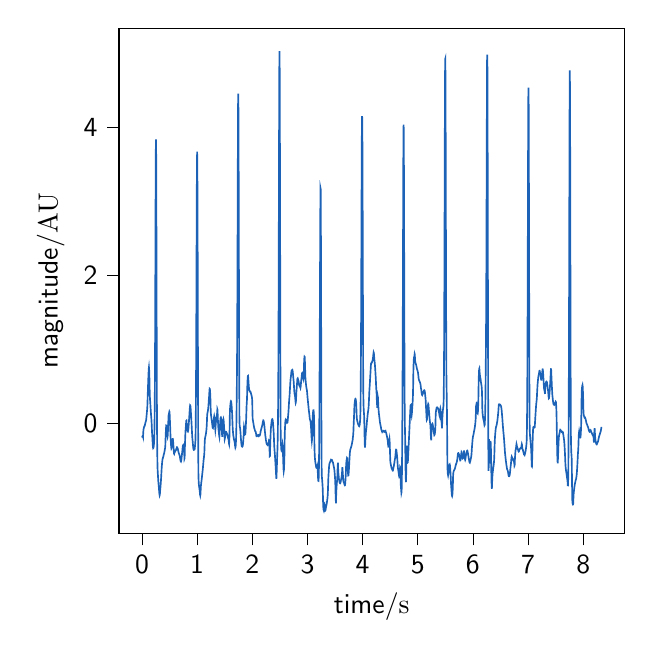
\begin{tikzpicture}
\pgfplotsset{
   every axis/.append style={
		font=\fontsize{10}{10}\sffamily},
	every non boxed x axis/.append style={
		x axis line style={->}
	},
	every non boxed y axis/.append style={
		y axis line style={->}
	},
	every non boxed z axis/.append style={
		z axis line style={->}
	}
}
\begin{axis}[
height=\figH,
tick align=outside,
tick pos=left,
width=\figW,
x grid style={white!69.0196078431373!black},
xlabel={time/$\si{\second}$},
xmin=-0.416499996185303, xmax=8.74649991989136,
xtick style={color=black},
y grid style={white!69.0196078431373!black},
ylabel={magnitude/\si{AU}},
ymin=-1.49265742897987, ymax=5.33461392521858,
ytick style={color=black},
ytick = {0, 2, 4},
yticklabels = {0, 2, 4},
xtick = {0, 1, 2, 3, 4, 5, 6, 7, 8},
xticklabels = {0, 1, 2, 3, 4, 5, 6, 7, 8},
]
\addplot [semithick, tud1b]
table {%
0 -0.177926599979401
0.00333333341404796 -0.182931125164032
0.00666666682809591 -0.18271903693676
0.00999999977648258 -0.177290320396423
0.0133333336561918 -0.171914026141167
0.0166666675359011 -0.17185927927494
0.0199999995529652 -0.182395115494728
0.0233333334326744 -0.124486193060875
0.0266666673123837 -0.092974916100502
0.0299999993294477 -0.0773232132196426
0.0333333350718021 -0.0669928640127182
0.0366666652262211 -0.0567148327827454
0.0399999991059303 -0.0464890599250793
0.0433333329856396 -0.0468534231185913
0.0466666668653488 -0.0420006960630417
0.0500000007450581 -0.0371996536850929
0.0533333346247673 -0.0271812453866005
0.0566666685044765 -0.0119451731443405
0.0599999986588955 -0.00202926993370056
0.0633333325386047 0.00783593207597733
0.0666666701436043 0.0176505446434021
0.0700000002980232 0.0221455693244934
0.0733333304524422 0.031859777867794
0.0766666680574417 0.0467935651540756
0.0799999982118607 0.072216123342514
0.0833333358168602 0.097589448094368
0.0866666659712791 0.128183484077454
0.0900000035762787 0.153460636734962
0.0933333337306976 0.178690195083618
0.0966666638851166 0.214410185813904
0.100000001490116 0.271160006523132
0.103333331644535 0.354208558797836
0.106666669249535 0.431942671537399
0.109999999403954 0.504362165927887
0.113333337008953 0.571468532085419
0.116666667163372 0.638530671596527
0.119999997317791 0.689742624759674
0.123333334922791 0.735642194747925
0.126666665077209 0.755155086517334
0.129999995231628 0.727205038070679
0.133333340287209 0.662331283092499
0.136666670441628 0.565802574157715
0.140000000596046 0.43235194683075
0.143333330750465 0.351552367210388
0.146666660904884 0.312867283821106
0.150000005960464 0.279413253068924
0.153333336114883 0.240654408931732
0.156666666269302 0.201859772205353
0.159999996423721 0.163029849529266
0.16333332657814 0.124165378510952
0.16666667163372 0.0905373394489288
0.170000001788139 0.062145821750164
0.173333331942558 0.0231838338077068
0.176666662096977 -0.0210775882005692
0.180000007152557 -0.0811755955219269
0.183333337306976 -0.13603363931179
0.186666667461395 -0.175113588571548
0.189999997615814 -0.219489395618439
0.193333327770233 -0.263891071081161
0.196666672825813 -0.303049117326736
0.200000002980232 -0.326425433158875
0.203333333134651 -0.339286357164383
0.20666666328907 -0.336363166570663
0.209999993443489 -0.328192114830017
0.213333338499069 -0.309504508972168
0.216666668653488 -0.285566598176956
0.219999998807907 -0.251109719276428
0.223333328962326 -0.185055837035179
0.226666674017906 -0.0557912550866604
0.230000004172325 0.131417885422707
0.233333334326744 0.43979948759079
0.236666664481163 0.900969564914703
0.239999994635582 1.52019691467285
0.243333339691162 2.25533199310303
0.246666669845581 3.01153230667114
0.25 3.62546014785767
0.253333330154419 3.83366441726685
0.256666660308838 3.76260423660278
0.259999990463257 3.21205687522888
0.263333320617676 2.27159667015076
0.266666680574417 1.2468273639679
0.270000010728836 0.411740839481354
0.273333340883255 -0.107206501066685
0.276666671037674 -0.367973148822784
0.280000001192093 -0.528628766536713
0.283333331346512 -0.626053810119629
0.286666661500931 -0.670786380767822
0.28999999165535 -0.710247039794922
0.293333321809769 -0.749703705310822
0.296666651964188 -0.789153814315796
0.300000011920929 -0.818059384822845
0.303333342075348 -0.846957743167877
0.306666672229767 -0.870578408241272
0.310000002384186 -0.904727339744568
0.313333332538605 -0.938865005970001
0.316666662693024 -0.96245276927948
0.319999992847443 -0.975490629673004
0.323333323001862 -0.967437922954559
0.326666653156281 -0.943562865257263
0.330000013113022 -0.909133672714233
0.333333343267441 -0.879957556724548
0.33666667342186 -0.850762963294983
0.340000003576279 -0.821548938751221
0.343333333730698 -0.787045955657959
0.346666663885117 -0.747253835201263
0.349999994039536 -0.702170312404633
0.353333324193954 -0.65706342458725
0.356666654348373 -0.617201864719391
0.360000014305115 -0.582585215568542
0.363333344459534 -0.553211092948914
0.366666674613953 -0.523810684680939
0.370000004768372 -0.504920363426208
0.373333334922791 -0.486002385616302
0.376666665077209 -0.477592259645462
0.379999995231628 -0.469152271747589
0.383333325386047 -0.460680782794952
0.386666655540466 -0.452178090810776
0.389999985694885 -0.443641841411591
0.393333345651627 -0.429803282022476
0.396666675806046 -0.421198964118958
0.400000005960464 -0.412560075521469
0.403333336114883 -0.403884440660477
0.406666666269302 -0.389903366565704
0.409999996423721 -0.375884354114532
0.41333332657814 -0.361827701330185
0.416666656732559 -0.347731411457062
0.419999986886978 -0.333595365285873
0.423333346843719 -0.303612470626831
0.426666676998138 -0.231435984373093
0.430000007152557 -0.164486512541771
0.433333337306976 -0.108032695949078
0.436666667461395 -0.0620744526386261
0.439999997615814 -0.0318793728947639
0.443333327770233 -0.0332539454102516
0.446666657924652 -0.0609288811683655
0.449999988079071 -0.0885589718818665
0.453333348035812 -0.116142719984055
0.456666678190231 -0.143680348992348
0.46000000834465 -0.171170920133591
0.463333338499069 -0.182807505130768
0.466666668653488 -0.168050795793533
0.469999998807907 -0.121631950139999
0.473333328962326 -0.0646262541413307
0.476666659116745 -0.0023028552532196
0.479999989271164 0.081146351993084
0.483333319425583 0.11195495724678
0.486666679382324 0.121737711131573
0.490000009536743 0.13157057762146
0.493333339691162 0.146723419427872
0.496666669845581 0.156658083200455
0.5 0.150837004184723
0.503333330154419 0.10291500389576
0.506666660308838 0.039237767457962
0.509999990463257 -0.0191186368465424
0.513333320617676 -0.0984991937875748
0.516666650772095 -0.162020623683929
0.519999980926514 -0.209682613611221
0.523333311080933 -0.252023249864578
0.526666641235352 -0.294311463832855
0.529999971389771 -0.326009184122086
0.533333361148834 -0.341847270727158
0.536666691303253 -0.336556762456894
0.540000021457672 -0.320675671100616
0.543333351612091 -0.29947304725647
0.54666668176651 -0.283487021923065
0.550000011920929 -0.262179642915726
0.553333342075348 -0.235550910234451
0.556666672229767 -0.214139059185982
0.560000002384186 -0.213751241564751
0.563333332538605 -0.23438772559166
0.566666662693024 -0.265510499477386
0.569999992847443 -0.30185079574585
0.573333323001862 -0.332870841026306
0.576666653156281 -0.374378025531769
0.579999983310699 -0.410565465688705
0.583333313465118 -0.415088057518005
0.586666643619537 -0.403753578662872
0.589999973773956 -0.397638469934464
0.593333303928375 -0.391473889350891
0.596666693687439 -0.390528917312622
0.600000023841858 -0.384266376495361
0.603333353996277 -0.377955704927444
0.606666684150696 -0.376866221427917
0.610000014305115 -0.370459914207458
0.613333344459534 -0.369276076555252
0.616666674613953 -0.362776547670364
0.620000004768372 -0.356231331825256
0.623333334922791 -0.344371169805527
0.626666665077209 -0.343004673719406
0.629999995231628 -0.336324602365494
0.633333325386047 -0.340139120817184
0.636666655540466 -0.338640928268433
0.639999985694885 -0.331831783056259
0.643333315849304 -0.335518538951874
0.646666646003723 -0.33916437625885
0.649999976158142 -0.348038047552109
0.653333306312561 -0.362141519784927
0.656666696071625 -0.370936512947083
0.660000026226044 -0.384962409734726
0.663333356380463 -0.393680930137634
0.666666686534882 -0.402363181114197
0.670000016689301 -0.411009281873703
0.673333346843719 -0.419619262218475
0.676666676998138 -0.42292594909668
0.680000007152557 -0.43146824836731
0.683333337306976 -0.439977616071701
0.686666667461395 -0.448454082012177
0.689999997615814 -0.467437714338303
0.693333327770233 -0.48112228512764
0.696666657924652 -0.500046372413635
0.699999988079071 -0.513671934604645
0.70333331823349 -0.516732156276703
0.706666648387909 -0.519765973091125
0.709999978542328 -0.512235879898071
0.713333308696747 -0.499410897493362
0.716666638851166 -0.481293767690659
0.720000028610229 -0.457884103059769
0.723333358764648 -0.434452772140503
0.726666688919067 -0.41099938750267
0.730000019073486 -0.387526750564575
0.733333349227905 -0.364034563302994
0.736666679382324 -0.335255593061447
0.740000009536743 -0.316996604204178
0.743333339691162 -0.298722386360168
0.746666669845581 -0.296239614486694
0.75 -0.293743252754211
0.753333330154419 -0.307039946317673
0.756666660308838 -0.325594544410706
0.759999990463257 -0.349406719207764
0.763333320617676 -0.37320938706398
0.766666650772095 -0.412809312343597
0.769999980926514 -0.478747427463531
0.773333311080933 -0.470912516117096
0.776666641235352 -0.368229061365128
0.779999971389771 -0.281347513198853
0.783333361148834 -0.205001354217529
0.786666691303253 -0.144459739327431
0.790000021457672 -0.099723257124424
0.793333351612091 -0.070792943239212
0.79666668176651 -0.0365952700376511
0.800000011920929 0.00286968518048525
0.803333342075348 0.0317942723631859
0.806666672229767 0.0343698784708977
0.810000002384186 5.73983415961266e-05
0.813333332538605 -0.0395305901765823
0.816666662693024 -0.0580490753054619
0.819999992847443 -0.0713066607713699
0.823333323001862 -0.0898424461483955
0.826666653156281 -0.103119902312756
0.829999983310699 -0.111139610409737
0.833333313465118 -0.113901667296886
0.836666643619537 -0.106139495968819
0.839999973773956 -0.0878541469573975
0.843333303928375 -0.0590461231768131
0.846666693687439 -0.0302536077797413
0.850000023841858 0.00379003584384918
0.853333353996277 0.0430838130414486
0.856666684150696 0.0770891457796097
0.860000014305115 0.116343982517719
0.863333344459534 0.155576527118683
0.866666674613953 0.19478714466095
0.870000004768372 0.223435953259468
0.873333334922791 0.241523295640945
0.876666665077209 0.238508492708206
0.879999995231628 0.219660922884941
0.883333325386047 0.190247774124146
0.886666655540466 0.150269463658333
0.889999985694885 0.1102614402771
0.893333315849304 0.0702240392565727
0.896666646003723 0.0248865894973278
0.899999976158142 -0.0204815939068794
0.903333306312561 -0.0711519047617912
0.906666696071625 -0.121855035424232
0.910000026226044 -0.167323529720306
0.913333356380463 -0.202288061380386
0.916666686534882 -0.226750880479813
0.920000016689301 -0.251249700784683
0.923333346843719 -0.281054735183716
0.926666676998138 -0.310897648334503
0.930000007152557 -0.335510492324829
0.933333337306976 -0.34962460398674
0.936666667461395 -0.35850915312767
0.939999997615814 -0.362165719270706
0.943333327770233 -0.360594928264618
0.946666657924652 -0.359066188335419
0.949999988079071 -0.357579588890076
0.95333331823349 -0.356136500835419
0.956666648387909 -0.344199568033218
0.959999978542328 -0.321769058704376
0.963333308696747 -0.288845002651215
0.966666638851166 -0.25596696138382
0.970000028610229 -0.228403836488724
0.973333358764648 -0.0849690735340118
0.976666688919067 0.184875547885895
0.980000019073486 0.565321624279022
0.983333349227905 1.06690740585327
0.986666679382324 1.68963205814362
0.990000009536743 2.39134359359741
0.993333339691162 3.05612206459045
0.996666669845581 3.51009082794189
1 3.66894435882568
1.00333333015442 3.52741360664368
1.00666666030884 3.08549809455872
1.00999999046326 2.26943135261536
1.01333332061768 1.3215879201889
1.01666665077209 0.373693346977234
1.01999998092651 -0.384568214416504
1.02333331108093 -0.679207682609558
1.02666664123535 -0.76840728521347
1.02999997138977 -0.815506637096405
1.03333330154419 -0.841582179069519
1.03666663169861 -0.862441062927246
1.03999996185303 -0.878083288669586
1.04333329200745 -0.893777966499329
1.04666662216187 -0.914794147014618
1.04999995231628 -0.941131949424744
1.0533332824707 -0.967522263526917
1.05666661262512 -0.978157997131348
1.05999994277954 -0.962501168251038
1.06333339214325 -0.920551538467407
1.06666672229767 -0.86811625957489
1.07000005245209 -0.83680933713913
1.07333338260651 -0.816092550754547
1.07666671276093 -0.795427620410919
1.08000004291534 -0.780083477497101
1.08333337306976 -0.754253029823303
1.08666670322418 -0.733742952346802
1.0900000333786 -0.708014905452728
1.09333336353302 -0.687606692314148
1.09666669368744 -0.661980330944061
1.10000002384186 -0.64167320728302
1.10333335399628 -0.616146922111511
1.1066666841507 -0.590670228004456
1.11000001430511 -0.559974193572998
1.11333334445953 -0.534595906734467
1.11666667461395 -0.503996968269348
1.12000000476837 -0.483984172344208
1.12333333492279 -0.464019417762756
1.12666666507721 -0.438832461833954
1.12999999523163 -0.413692474365234
1.13333332538605 -0.356984257698059
1.13666665554047 -0.279246211051941
1.13999998569489 -0.227897986769676
1.1433333158493 -0.202939689159393
1.14666664600372 -0.188563197851181
1.14999997615814 -0.179499745368958
1.15333330631256 -0.170478582382202
1.15666663646698 -0.156230896711349
1.1599999666214 -0.142024502158165
1.16333329677582 -0.122590601444244
1.16666662693024 -0.103196308016777
1.16999995708466 -0.0785728618502617
1.17333328723907 -0.0434502065181732
1.17666661739349 0.00217237323522568
1.17999994754791 0.0741030648350716
1.18333327770233 0.119652047753334
1.18666660785675 0.133550375699997
1.19000005722046 0.147414028644562
1.19333338737488 0.15597477555275
1.1966667175293 0.175040170550346
1.20000004768372 0.19407220184803
1.20333337783813 0.218341901898384
1.20666670799255 0.253119140863419
1.21000003814697 0.293135404586792
1.21333336830139 0.327852696180344
1.21666669845581 0.357273548841476
1.22000002861023 0.397204697132111
1.22333335876465 0.442378908395767
1.22666668891907 0.466450691223145
1.23000001907349 0.464153647422791
1.23333334922791 0.440756529569626
1.23666667938232 0.401530146598816
1.24000000953674 0.357012122869492
1.24333333969116 0.270322203636169
1.24666666984558 0.162536054849625
1.25 0.123228892683983
1.25333333015442 0.0997101664543152
1.25666666030884 0.0814446806907654
1.25999999046326 0.063163049519062
1.26333332061768 0.0448672249913216
1.26666665077209 0.0265568271279335
1.26999998092651 0.00823476910591125
1.27333331108093 -0.010099321603775
1.27666664123535 -0.0337124764919281
1.27999997138977 -0.0573360472917557
1.28333330154419 -0.0651600211858749
1.28666663169861 -0.0677223280072212
1.28999996185303 -0.0544843561947346
1.29333329200745 -0.0307140722870827
1.29666662216187 -0.0016779750585556
1.29999995231628 0.0168169718235731
1.3033332824707 0.0511164516210556
1.30666661262512 0.0801454558968544
1.30999994277954 0.0933684483170509
1.31333339214325 0.0802474990487099
1.31666672229767 0.0513212457299232
1.32000005245209 0.0171292573213577
1.32333338260651 -0.0170583706349134
1.32666671276093 -0.067047156393528
1.33000004291534 -0.0906848385930061
1.33333337306976 -0.0668938010931015
1.33666670322418 -0.0220180824398994
1.3400000333786 0.0070607028901577
1.34333336353302 0.030881155282259
1.34666669368744 0.0547123998403549
1.35000002384186 0.0732878819108009
1.35333335399628 0.0866086184978485
1.3566666841507 0.0999442040920258
1.36000001430511 0.118563711643219
1.36333334445953 0.142469614744186
1.36666667461395 0.18746991455555
1.37000000476837 0.179798901081085
1.37333333492279 0.103649601340294
1.37666666507721 0.0433291085064411
1.37999999523163 -0.0064319483935833
1.38333332538605 -0.0509007424116135
1.38666665554047 -0.0795395821332932
1.38999998569489 -0.102883845567703
1.3933333158493 -0.12093386054039
1.39666664600372 -0.144225895404816
1.39999997615814 -0.172760307788849
1.40333330631256 -0.185458451509476
1.40666663646698 -0.15070652961731
1.4099999666214 -0.0790408924221992
1.41333329677582 -0.0389591418206692
1.41666662693024 -0.00411373376846313
1.41999995708466 0.0307640060782433
1.42333328723907 0.0604063048958778
1.42666661739349 0.0742758885025978
1.42999994754791 0.0776429921388626
1.43333327770233 0.0705080032348633
1.43666660785675 0.052871011197567
1.44000005722046 0.0300028324127197
1.44333338737488 -0.00336482375860214
1.4466667175293 -0.0683076679706573
1.45000004768372 -0.138480499386787
1.45333337783813 -0.166460484266281
1.45666670799255 -0.18386110663414
1.46000003814697 -0.111646719276905
1.46333336830139 -0.0499286204576492
1.46666669845581 -0.0145123675465584
1.47000002861023 0.0209477171301842
1.47333335876465 0.0459138825535774
1.47666668891907 0.0551171973347664
1.48000001907349 0.0432902127504349
1.48333334922791 0.0104326829314232
1.48666667938232 -0.0276473164558411
1.49000000953674 -0.0709499567747116
1.49333333969116 -0.11420489102602
1.49666666984558 -0.183757394552231
1.5 -0.216378390789032
1.50333333015442 -0.206799015402794
1.50666666030884 -0.186632230877876
1.50999999046326 -0.171685293316841
1.51333332061768 -0.156688466668129
1.51666665077209 -0.136372864246368
1.51999998092651 -0.121275641024113
1.52333331108093 -0.116665929555893
1.52666664123535 -0.117274180054665
1.52999997138977 -0.123100481927395
1.53333330154419 -0.128875181078911
1.53666663169861 -0.134598255157471
1.53999996185303 -0.140269592404366
1.54333329200745 -0.145889028906822
1.54666662216187 -0.151456207036972
1.54999995231628 -0.16224017739296
1.5533332824707 -0.178240850567818
1.55666661262512 -0.188920110464096
1.55999994277954 -0.199546843767166
1.56333339214325 -0.204852014780045
1.56666672229767 -0.215373709797859
1.57000005245209 -0.225842863321304
1.57333338260651 -0.246797531843185
1.57666671276093 -0.272968828678131
1.58000004291534 -0.283280611038208
1.58333337306976 -0.24611896276474
1.58666670322418 -0.161483943462372
1.5900000333786 -0.0346447825431824
1.59333336353302 0.129129350185394
1.59666669368744 0.19284400343895
1.60000002384186 0.230264991521835
1.60333335399628 0.251930058002472
1.6066666841507 0.273646146059036
1.61000001430511 0.290144234895706
1.61333334445953 0.296154618263245
1.61666667461395 0.291676998138428
1.62000000476837 0.276711195707321
1.62333333492279 0.25125715136528
1.62666666507721 0.220583066344261
1.62999999523163 0.184688493609428
1.63333332538605 0.143573254346848
1.63666665554047 0.0814302414655685
1.63999998569489 0.0193342864513397
1.6433333158493 -0.0427144765853882
1.64666664600372 -0.0889099091291428
1.64999997615814 -0.119251802563667
1.65333330631256 -0.149548724293709
1.65666663646698 -0.169262409210205
1.6599999666214 -0.183662980794907
1.66333329677582 -0.198019236326218
1.66666662693024 -0.212332874536514
1.66999995708466 -0.226603657007217
1.67333328723907 -0.235563457012177
1.67666661739349 -0.249751016497612
1.67999994754791 -0.258629262447357
1.68333327770233 -0.27273628115654
1.68666660785675 -0.297342121601105
1.69000005722046 -0.316640436649323
1.69333338737488 -0.330632299184799
1.6966667175293 -0.323511064052582
1.70000004768372 -0.30054584145546
1.70333337783813 -0.256469368934631
1.70666670799255 -0.196551561355591
1.71000003814697 -0.0997167378664017
1.71333336830139 0.0445730611681938
1.71666669845581 0.262661010026932
1.72000002861023 0.507124960422516
1.72333335876465 0.814847648143768
1.72666668891907 1.23851919174194
1.73000001907349 1.81502044200897
1.73333334922791 2.53381323814392
1.73666667938232 3.31059169769287
1.74000000953674 4.01889991760254
1.74333333969116 4.42689800262451
1.74666666984558 4.45028257369995
1.75 4.13120317459106
1.75333333015442 3.35374212265015
1.75666666030884 2.37081003189087
1.75999999046326 1.39316725730896
1.76333332061768 0.594689965248108
1.76666665077209 0.0965660810470581
1.76999998092651 -0.0221720039844513
1.77333331108093 -0.0460510142147541
1.77666664123535 -0.0593772307038307
1.77999997138977 -0.0726883113384247
1.78333330154419 -0.101794220507145
1.78666663169861 -0.130888000130653
1.78999996185303 -0.1705082654953
1.79333329200745 -0.204848974943161
1.79666662216187 -0.233912646770477
1.79999995231628 -0.262968361377716
1.8033332824707 -0.286747694015503
1.80666661262512 -0.305251717567444
1.80999994277954 -0.313213884830475
1.81333339214325 -0.31590336561203
1.81666672229767 -0.318589717149734
1.82000005245209 -0.316004991531372
1.82333338260651 -0.313420742750168
1.82666671276093 -0.305568039417267
1.83000004291534 -0.292447507381439
1.83333337306976 -0.268791615962982
1.83666670322418 -0.239870473742485
1.8400000333786 -0.20041660964489
1.84333336353302 -0.160968661308289
1.84666669368744 -0.0846435651183128
1.85000002384186 -0.0504791252315044
1.85333335399628 -0.0637454316020012
1.8566666841507 -0.0980979353189468
1.86000001430511 -0.116653576493263
1.86333334445953 -0.129952892661095
1.86666667461395 -0.143265932798386
1.87000000476837 -0.151324212551117
1.87333333492279 -0.148858830332756
1.87666666507721 -0.125334143638611
1.87999999523163 -0.0807511806488037
1.88333332538605 -0.0309175029397011
1.88666665554047 0.018897732719779
1.88999998569489 0.0792297869920731
1.8933333158493 0.155348047614098
1.89666664600372 0.231443598866463
1.89999997615814 0.275902658700943
1.90333330631256 0.315067648887634
1.90666663646698 0.391091078519821
1.9099999666214 0.498702168464661
1.91333329677582 0.569403946399689
1.91666662693024 0.608462929725647
1.91999995708466 0.636955380439758
1.92333328723907 0.639073491096497
1.92666661739349 0.614815175533295
1.92999994754791 0.574718296527863
1.93333327770233 0.539858639240265
1.93666660785675 0.49969682097435
1.94000005722046 0.475308179855347
1.94333338737488 0.456153392791748
1.9466667175293 0.442232131958008
1.95000004768372 0.438813328742981
1.95333337783813 0.435357064008713
1.95666670799255 0.431862652301788
1.96000003814697 0.423060655593872
1.96333336830139 0.419489055871964
1.96666669845581 0.415877163410187
1.97000002861023 0.417493313550949
1.97333335876465 0.408530116081238
1.97666668891907 0.39952552318573
1.98000001907349 0.390478014945984
1.98333334922791 0.381387025117874
1.98666667938232 0.372252225875854
1.99000000953674 0.363073527812958
1.99333333969116 0.348580330610275
1.99666666984558 0.328772842884064
2 0.277304977178574
2.00333333015442 0.136217683553696
2.00666666030884 0.063580185174942
2.00999999046326 0.0383165776729584
2.01333332061768 0.028811901807785
2.01666665077209 0.0139902234077454
2.01999998092651 -0.000880599021911621
2.02333331108093 -0.0158005654811859
2.02666664123535 -0.0307700484991074
2.02999997138977 -0.0457891002297401
2.03333330154419 -0.0608586445450783
2.03666663169861 -0.0707094073295593
2.03999996185303 -0.0753421857953072
2.04333329200745 -0.0852948203682899
2.04666662216187 -0.0952989533543587
2.04999995231628 -0.105354577302933
2.0533332824707 -0.110192894935608
2.05666661262512 -0.115082934498787
2.05999994277954 -0.114756152033806
2.06333327293396 -0.119750559329987
2.06666660308838 -0.135335192084312
2.0699999332428 -0.150972247123718
2.07333326339722 -0.166661828756332
2.07666659355164 -0.177134871482849
2.07999992370605 -0.177122384309769
2.08333325386047 -0.171893432736397
2.08666658401489 -0.171985998749733
2.08999991416931 -0.172131031751633
2.09333324432373 -0.172328561544418
2.09666657447815 -0.172578349709511
2.09999990463257 -0.167611464858055
2.10333323478699 -0.162696570158005
2.10666656494141 -0.157833620905876
2.10999989509583 -0.158291667699814
2.11333322525024 -0.164070174098015
2.11666655540466 -0.16463103890419
2.11999988555908 -0.170512080192566
2.1233332157135 -0.165906220674515
2.1266667842865 -0.166620060801506
2.13000011444092 -0.167383968830109
2.13333344459534 -0.168197900056839
2.13666677474976 -0.163792818784714
2.14000010490417 -0.159436732530594
2.14333343505859 -0.149860590696335
2.14666676521301 -0.135063976049423
2.15000009536743 -0.115046858787537
2.15333342552185 -0.105615094304085
2.15666675567627 -0.0962310135364532
2.16000008583069 -0.086893267929554
2.16333341598511 -0.077601782977581
2.16666674613953 -0.0683565437793732
2.17000007629395 -0.0591560378670692
2.17333340644836 -0.0500007271766663
2.17666673660278 -0.0408889949321747
2.1800000667572 -0.0318207591772079
2.18333339691162 -0.0227954387664795
2.18666672706604 -0.00854393839836121
2.19000005722046 0.010935515165329
2.19333338737488 0.0198353603482246
2.1966667175293 0.0286955162882805
2.20000004768372 0.0375154130160809
2.20333337783813 0.035759013146162
2.20666670799255 0.0234264209866524
2.21000003814697 0.0110564008355141
2.21333336830139 -0.001350998878479
2.21666669845581 -0.0190625935792923
2.22000002861023 -0.0420783460140228
2.22333335876465 -0.0703981295228004
2.22666668891907 -0.0934824347496033
2.23000001907349 -0.121867671608925
2.23333334922791 -0.145015686750412
2.23666667938232 -0.168194681406021
2.24000000953674 -0.186135560274124
2.24333333969116 -0.204104840755463
2.24666666984558 -0.227371454238892
2.25 -0.240128293633461
2.25333333015442 -0.252911627292633
2.25666666030884 -0.265719711780548
2.25999999046326 -0.278552412986755
2.26333332061768 -0.286139756441116
2.26666665077209 -0.288481712341309
2.26999998092651 -0.290844559669495
2.27333331108093 -0.293228179216385
2.27666664123535 -0.295631587505341
2.27999997138977 -0.287516742944717
2.28333330154419 -0.284688651561737
2.28666663169861 -0.281876474618912
2.28999996185303 -0.27908006310463
2.29333329200745 -0.271030336618423
2.29666662216187 -0.268262416124344
2.29999995231628 -0.25496917963028
2.3033332824707 -0.231149539351463
2.30666661262512 -0.233686566352844
2.30999994277954 -0.304730445146561
2.31333327293396 -0.375781863927841
2.31666660308838 -0.446840763092041
2.3199999332428 -0.444140732288361
2.32333326339722 -0.346602737903595
2.32666659355164 -0.259607076644897
2.32999992370605 -0.188421666622162
2.33333325386047 -0.12777741253376
2.33666658401489 -0.0829403400421143
2.33999991416931 -0.0486422888934612
2.34333324432373 -0.0248802490532398
2.34666657447815 -0.00111705716699362
2.34999990463257 0.0173812732100487
2.35333323478699 0.0358838550746441
2.35666656494141 0.0438537150621414
2.35999989509583 0.0518289878964424
2.36333322525024 0.0545436441898346
2.36666655540466 0.0519968122243881
2.36999988555908 0.038922443985939
2.3733332157135 0.0205886960029602
2.3766667842865 -0.0082705058157444
2.38000011444092 -0.0423860512673855
2.38333344459534 -0.0764878988265991
2.38666677474976 -0.115844950079918
2.39000010490417 -0.1551853120327
2.39333343505859 -0.220854014158249
2.39666676521301 -0.286505848169327
2.40000009536743 -0.331062793731689
2.40333342552185 -0.365061044692993
2.40666675567627 -0.39903849363327
2.41000008583069 -0.427725195884705
2.41333341598511 -0.466928124427795
2.41666674613953 -0.506106495857239
2.42000007629395 -0.54526025056839
2.42333340644836 -0.584389328956604
2.42666673660278 -0.628760099411011
2.4300000667572 -0.673104345798492
2.43333339691162 -0.727957427501678
2.43666672706604 -0.751168012619019
2.44000005722046 -0.716388523578644
2.44333338737488 -0.634156942367554
2.4466667175293 -0.562431514263153
2.45000004768372 -0.480136215686798
2.45333337783813 -0.408344745635986
2.45666670799255 -0.35232675075531
2.46000003814697 -0.254120767116547
2.46333336830139 -0.12426546216011
2.46666669845581 0.105738557875156
2.47000002861023 0.393739223480225
2.47333335876465 0.845117568969727
2.47666668891907 1.50729513168335
2.48000001907349 2.36446666717529
2.48333334922791 3.32178950309753
2.48666667938232 4.19484853744507
2.49000000953674 4.79922962188721
2.49333333969116 5.02428340911865
2.49666666984558 4.78570699691772
2.5 4.08876895904541
2.50333333015442 3.05465698242188
2.50666666030884 1.86778903007507
2.50999999046326 0.775808334350586
2.51333332061768 -0.0105237886309624
2.51666665077209 -0.222486019134521
2.51999998092651 -0.281600326299667
2.52333331108093 -0.324859917163849
2.52666664123535 -0.357533752918243
2.52999997138977 -0.369083791971207
2.53333330154419 -0.364777833223343
2.53666663169861 -0.360422939062119
2.53999996185303 -0.35074970126152
2.54333329200745 -0.341027110815048
2.54666662216187 -0.325985431671143
2.54999995231628 -0.295086085796356
2.5533332824707 -0.311557292938232
2.55666661262512 -0.417551189661026
2.55999994277954 -0.491879552602768
2.56333327293396 -0.566156506538391
2.56666660308838 -0.624574899673462
2.5699999332428 -0.65132749080658
2.57333326339722 -0.635875821113586
2.57666659355164 -0.588757991790771
2.57999992370605 -0.5205118060112
2.58333325386047 -0.425868213176727
2.58666658401489 -0.236329764127731
2.58999991416931 -0.120505154132843
2.59333324432373 -0.0625872537493706
2.59666657447815 -0.0151548534631729
2.59999990463257 0.0270610451698303
2.60333323478699 0.0429843664169312
2.60666656494141 0.0484220832586288
2.60999989509583 0.0433742254972458
2.61333322525024 0.038378581404686
2.61666655540466 0.0387041121721268
2.61999988555908 0.0338126569986343
2.6233332157135 0.0289732813835144
2.6266667842865 0.0241854265332222
2.63000011444092 0.0141800567507744
2.63333344459534 0.0042262002825737
2.63666677474976 0.00486146658658981
2.64000010490417 0.0160853192210197
2.64333343505859 0.0431667268276215
2.64666676521301 0.0702983289957047
2.65000009536743 0.102749146521091
2.65333342552185 0.129980146884918
2.65666675567627 0.162529334425926
2.66000008583069 0.200396686792374
2.66333341598511 0.248850509524345
2.66666674613953 0.286813825368881
2.67000007629395 0.319555580615997
2.67333340644836 0.352344810962677
2.67666673660278 0.379911154508591
2.6800000667572 0.42333060503006
2.68333339691162 0.466795533895493
2.68666672706604 0.510306000709534
2.69000005722046 0.553860306739807
2.69333338737488 0.586920917034149
2.6966667175293 0.609486222267151
2.70000004768372 0.62682580947876
2.70333337783813 0.649475634098053
2.70666670799255 0.677435994148254
2.71000003814697 0.700167894363403
2.71333336830139 0.71240246295929
2.71666669845581 0.714137554168701
2.72000002861023 0.71591192483902
2.72333335876465 0.717723488807678
2.72666668891907 0.719572782516479
2.73000001907349 0.710919678211212
2.73333334922791 0.697033047676086
2.73666667938232 0.67264324426651
2.74000000953674 0.643019020557404
2.74333333969116 0.613427221775055
2.74666666984558 0.589136719703674
2.75 0.564878463745117
2.75333333015442 0.530112683773041
2.75666666030884 0.490106821060181
2.75999999046326 0.444860756397247
2.76333332061768 0.415449678897858
2.76666665077209 0.3966044485569
2.76999998092651 0.383053481578827
2.77333331108093 0.369527697563171
2.77666664123535 0.356026977300644
2.77999997138977 0.326741576194763
2.78333330154419 0.292210340499878
2.78666663169861 0.273506551980972
2.78999996185303 0.281168252229691
2.79333329200745 0.320464372634888
2.79666662216187 0.375584930181503
2.79999995231628 0.425453871488571
2.8033332824707 0.454263031482697
2.80666661262512 0.488357484340668
2.80999994277954 0.522466242313385
2.81333327293396 0.556587338447571
2.81666660308838 0.590720653533936
2.8199999332428 0.603790044784546
2.82333326339722 0.606330573558807
2.82666659355164 0.598342180252075
2.82999992370605 0.585092782974243
2.83333325386047 0.577120363712311
2.83666658401489 0.574421942234039
2.83999991416931 0.566460311412811
2.84333324432373 0.547963440418243
2.84666657447815 0.529470324516296
2.84999990463257 0.510977864265442
2.85333323478699 0.503024101257324
2.85666656494141 0.500338852405548
2.85999989509583 0.497653037309647
2.86333322525024 0.494963645935059
2.86666655540466 0.487002521753311
2.86999988555908 0.48430472612381
2.8733332157135 0.47633308172226
2.8766667842865 0.489429712295532
2.88000011444092 0.513056457042694
2.88333344459534 0.547212302684784
2.88666677474976 0.570820987224579
2.89000010490417 0.594417691230774
2.89333343505859 0.612733244895935
2.89666676521301 0.636305630207062
2.90000009536743 0.659863829612732
2.90333342552185 0.678136944770813
2.90666675567627 0.680586695671082
2.91000008583069 0.67775022983551
2.91333341598511 0.66435843706131
2.91666674613953 0.645677447319031
2.92000007629395 0.626976191997528
2.92333340644836 0.602985680103302
2.92666673660278 0.594779133796692
2.9300000667572 0.618164360523224
2.93333339691162 0.673138856887817
2.93666672706604 0.759703278541565
2.94000005722046 0.840971767902374
2.94333338737488 0.874792277812958
2.9466667175293 0.898046910762787
2.95000004768372 0.894928514957428
2.95333337783813 0.849627614021301
2.95666670799255 0.783220946788788
2.96000003814697 0.679898977279663
2.96333336830139 0.613428771495819
2.96666669845581 0.57853889465332
2.97000002861023 0.554153203964233
2.97333335876465 0.524463832378387
2.97666668891907 0.505277812480927
2.98000001907349 0.486054807901382
2.98333334922791 0.472063839435577
2.98666667938232 0.458035796880722
2.99000000953674 0.443969249725342
2.99333333969116 0.424593806266785
2.99666666984558 0.394640445709229
3 0.36464649438858
3.00333333015442 0.334611892700195
3.00666666030884 0.309803783893585
3.00999999046326 0.28495317697525
3.01333332061768 0.260059922933578
3.01666665077209 0.235122874379158
3.01999998092651 0.210140958428383
3.02333331108093 0.185114145278931
3.02666664123535 0.165310919284821
3.02999997138977 0.145462155342102
3.03333330154419 0.125566452741623
3.03666663169861 0.100354753434658
3.03999996185303 0.0750956386327744
3.04333329200745 0.0550580285489559
3.04666662216187 0.0455101132392883
3.04999995231628 0.0411821231245995
3.0533332824707 0.0315359830856323
3.05666661262512 0.0165716782212257
3.05999994277954 -0.00898081809282303
3.06333327293396 -0.039852499961853
3.06666660308838 -0.0813126787543297
3.0699999332428 -0.128092408180237
3.07333326339722 -0.174923166632652
3.07666659355164 -0.216536372900009
3.07999992370605 -0.242394015192986
3.08333325386047 -0.220881998538971
3.08666658401489 -0.162538900971413
3.08999991416931 -0.0779026746749878
3.09333324432373 0.0435645207762718
3.09666657447815 0.0964822620153427
3.09999990463257 0.133540481328964
3.10333323478699 0.160008266568184
3.10666656494141 0.17588546872139
3.10999989509583 0.175903081893921
3.11333322525024 0.154792085289955
3.11666655540466 0.123090520501137
3.11999988555908 0.0755294412374496
3.1233332157135 -0.0827335715293884
3.1266667842865 -0.293739050626755
3.13000011444092 -0.394147455692291
3.13333344459534 -0.447186708450317
3.13666677474976 -0.484470963478088
3.14000010490417 -0.505999863147736
3.14333343505859 -0.527580380439758
3.14666676521301 -0.543943345546722
3.15000009536743 -0.555088639259338
3.15333342552185 -0.571553707122803
3.15666675567627 -0.588069319725037
3.16000008583069 -0.599366664886475
3.16333341598511 -0.605445086956024
3.16666674613953 -0.606303811073303
3.17000007629395 -0.601942896842957
3.17333340644836 -0.597631454467773
3.17666673660278 -0.593368113040924
3.1800000667572 -0.583883941173553
3.18333339691162 -0.574447512626648
3.18666672706604 -0.644094228744507
3.19000005722046 -0.703249156475067
3.19333338737488 -0.751912891864777
3.1966667175293 -0.779545843601227
3.20000004768372 -0.780879497528076
3.20333337783813 -0.750643253326416
3.20666670799255 -0.688836991786957
3.21000003814697 -0.511155843734741
3.21333336830139 -0.20706182718277
3.21666669845581 0.207639902830124
3.22000002861023 0.690796554088593
3.22333335876465 1.2107959985733
3.22666668891907 1.76236855983734
3.23000001907349 2.34024715423584
3.23333334922791 2.8759343624115
3.23666667938232 3.17447781562805
3.24000000953674 3.1621105670929
3.24333333969116 2.78087615966797
3.24666666984558 1.9412008523941
3.25 0.94868803024292
3.25333333015442 0.0457142107188702
3.25666666030884 -0.556958317756653
3.25999999046326 -0.706527888774872
3.26333332061768 -0.740210890769958
3.26666665077209 -0.768656730651855
3.26999998092651 -0.802400946617126
3.27333331108093 -0.836174488067627
3.27666664123535 -0.880515277385712
3.27999997138977 -0.961765885353088
3.28333330154419 -1.064120054245
3.28666663169861 -1.12434673309326
3.28999996185303 -1.16352224349976
3.29333329200745 -1.17110812664032
3.29666662216187 -1.14710211753845
3.29999995231628 -1.11784863471985
3.3033332824707 -1.0886162519455
3.30666661262512 -1.08574962615967
3.30999994277954 -1.11451601982117
3.31333327293396 -1.13803052902222
3.31666660308838 -1.15629279613495
3.3199999332428 -1.16930282115936
3.32333326339722 -1.18232691287994
3.32666659355164 -1.17955768108368
3.32999992370605 -1.1662632226944
3.33333325386047 -1.14771246910095
3.33666658401489 -1.1344405412674
3.33999991416931 -1.12117910385132
3.34333324432373 -1.11319446563721
3.34666657447815 -1.0999493598938
3.34999990463257 -1.08670973777771
3.35333323478699 -1.0682065486908
3.35666656494141 -1.0497077703476
3.35999989509583 -1.03121316432953
3.36333322525024 -1.01271998882294
3.36666655540466 -0.983690917491913
3.36999988555908 -0.944122910499573
3.3733332157135 -0.867671847343445
3.3766667842865 -0.785948693752289
3.38000011444092 -0.725298583507538
3.38333344459534 -0.685720264911652
3.38666677474976 -0.646137833595276
3.39000010490417 -0.611817181110382
3.39333343505859 -0.577489197254181
3.39666676521301 -0.558960855007172
3.40000009536743 -0.545692026615143
3.40333342552185 -0.537680804729462
3.40666675567627 -0.529658019542694
3.41000008583069 -0.526891708374023
3.41333341598511 -0.52411276102066
3.41666674613953 -0.516049146652222
3.42000007629395 -0.507969915866852
3.42333340644836 -0.505144000053406
3.42666673660278 -0.497031301259995
3.4300000667572 -0.499437063932419
3.43333339691162 -0.501823127269745
3.43666672706604 -0.498920440673828
3.44000005722046 -0.501264214515686
3.44333338737488 -0.49831634759903
3.4466667175293 -0.500613987445831
3.45000004768372 -0.508156895637512
3.45333337783813 -0.515673577785492
3.45666670799255 -0.523164629936218
3.46000003814697 -0.530627608299255
3.46333336830139 -0.532794117927551
3.46666669845581 -0.545468747615814
3.47000002861023 -0.5581134557724
3.47333335876465 -0.570727229118347
3.47666668891907 -0.583310127258301
3.48000001907349 -0.59585964679718
3.48333334922791 -0.608376502990723
3.48666667938232 -0.620858430862427
3.49000000953674 -0.643844127655029
3.49333333969116 -0.67206221818924
3.49666666984558 -0.705512821674347
3.5 -0.738926112651825
3.50333333015442 -0.782840013504028
3.50666666030884 -0.853059589862823
3.50999999046326 -0.954853713512421
3.51333332061768 -1.0302631855011
3.51666665077209 -1.08455562591553
3.51999998092651 -0.99654233455658
3.52333331108093 -0.924293994903564
3.52666664123535 -0.878347814083099
3.52999997138977 -0.84289687871933
3.53333330154419 -0.807401299476624
3.53666663169861 -0.78239917755127
3.53999996185303 -0.757352471351624
3.54333329200745 -0.69010728597641
3.54666662216187 -0.612278401851654
3.54999995231628 -0.566016495227814
3.5533332824707 -0.5355144739151
3.55666661262512 -0.615614533424377
3.55999994277954 -0.669321060180664
3.56333327293396 -0.691365003585815
3.56666660308838 -0.718629002571106
3.5699999332428 -0.745844125747681
3.57333326339722 -0.762471437454224
3.57666659355164 -0.779048502445221
3.57999992370605 -0.790306270122528
3.58333325386047 -0.801513671875
3.58666658401489 -0.807400941848755
3.58999991416931 -0.813237071037292
3.59333324432373 -0.813752830028534
3.59666657447815 -0.808948159217834
3.59999990463257 -0.798822462558746
3.60333323478699 -0.788645029067993
3.60666656494141 -0.773146331310272
3.60999989509583 -0.762864530086517
3.61333322525024 -0.752530336380005
3.61666655540466 -0.736874639987946
3.61999988555908 -0.721166610717773
3.6233332157135 -0.705405950546265
3.6266667842865 -0.679054796695709
3.63000011444092 -0.626305937767029
3.63333344459534 -0.594580709934235
3.63666677474976 -0.620762228965759
3.64000010490417 -0.673236489295959
3.64333343505859 -0.704582273960114
3.64666676521301 -0.741145014762878
3.65000009536743 -0.772386491298676
3.65333342552185 -0.793038189411163
3.65666675567627 -0.797831058502197
3.66000008583069 -0.802572250366211
3.66333341598511 -0.807262122631073
3.66666674613953 -0.817170083522797
3.67000007629395 -0.827027261257172
3.67333340644836 -0.831564605236053
3.67666673660278 -0.841320991516113
3.6800000667572 -0.840489506721497
3.68333339691162 -0.829070389270782
3.68666672706604 -0.796525597572327
3.69000005722046 -0.763932406902313
3.69333338737488 -0.720752358436584
3.6966667175293 -0.67225569486618
3.70000004768372 -0.592096924781799
3.70333337783813 -0.543505609035492
3.70666670799255 -0.521212816238403
3.71000003814697 -0.498873978853226
3.71333336830139 -0.481758058071136
3.71666669845581 -0.469866633415222
3.72000002861023 -0.473737269639969
3.72333335876465 -0.514447689056396
3.72666668891907 -0.570921301841736
3.73000001907349 -0.606276750564575
3.73333334922791 -0.652128100395203
3.73666667938232 -0.687400043010712
3.74000000953674 -0.706823587417603
3.74333333969116 -0.705131649971008
3.74666666984558 -0.682324230670929
3.75 -0.648939549922943
3.75333333015442 -0.604978799819946
3.75666666030884 -0.566250622272491
3.75999999046326 -0.511678993701935
3.76333332061768 -0.467609792947769
3.76666665077209 -0.428774058818817
3.76999998092651 -0.39517405629158
3.77333331108093 -0.372078865766525
3.77666664123535 -0.35948857665062
3.77999997138977 -0.35213577747345
3.78333330154419 -0.344753116369247
3.78666663169861 -0.337340652942657
3.78999996185303 -0.329899311065674
3.79333329200745 -0.317160099744797
3.79666662216187 -0.309663653373718
3.79999995231628 -0.302141040563583
3.8033332824707 -0.289324164390564
3.80666661262512 -0.276482105255127
3.80999994277954 -0.26361671090126
3.81333327293396 -0.250729769468307
3.81666660308838 -0.243090450763702
3.8199999332428 -0.224891766905785
3.82333326339722 -0.201405495405197
3.82666659355164 -0.177900776267052
3.82999992370605 -0.149109587073326
3.83333325386047 -0.115032017230988
3.83666658401489 -0.0440558716654778
3.83999991416931 0.0163956992328167
3.84333324432373 0.0663225948810577
3.84666657447815 0.132069826126099
3.84999990463257 0.203096434473991
3.85333323478699 0.247788175940514
3.85666656494141 0.276682078838348
3.85999989509583 0.295047014951706
3.86333322525024 0.313418090343475
3.86666655540466 0.326527178287506
3.86999988555908 0.329102218151093
3.8733332157135 0.326413035392761
3.8766667842865 0.318456768989563
3.88000011444092 0.294695198535919
3.88333344459534 0.265665292739868
3.88666677474976 0.220828950405121
3.89000010490417 0.14437609910965
3.89333343505859 0.0889977738261223
3.89666676521301 0.0599600188434124
3.90000009536743 0.0414566472172737
3.90333342552185 0.0282156337052584
3.90666675567627 0.0202368851751089
3.91000008583069 0.0122503321617842
3.91333341598511 -0.00101315230131149
3.91666674613953 -0.00901848636567593
3.92000007629395 -0.0170347820967436
3.92333340644836 -0.0197931192815304
3.92666673660278 -0.0278335213661194
3.9300000667572 -0.0358889363706112
3.93333339691162 -0.0386904254555702
3.93666672706604 -0.0362380966544151
3.94000005722046 -0.0390728339552879
3.94333338737488 -0.03138767182827
3.9466667175293 -0.0237216353416443
3.95000004768372 -0.00553679838776588
3.95333337783813 0.0231640879064798
3.95666670799255 0.0623818039894104
3.96000003814697 0.133189722895622
3.96333336830139 0.283009797334671
3.96666669845581 0.564529597759247
3.97000002861023 0.96194189786911
3.97333335876465 1.50686013698578
3.97666668891907 2.16766977310181
3.98000001907349 2.87060213088989
3.98333334922791 3.51027727127075
3.98666667938232 3.97604393959045
3.99000000953674 4.14671516418457
3.99333333969116 4.1276683807373
3.99666666984558 3.80825448036194
4 3.17266607284546
4.003333568573 2.35789680480957
4.00666666030884 1.50093936920166
4.01000022888184 0.765133142471313
4.01333332061768 0.377046078443527
4.01666688919067 0.252372324466705
4.01999998092651 0.185618713498116
4.02333354949951 0.145171076059341
4.02666664123535 0.11522164940834
4.03000020980835 0.0483491756021976
4.03333330154419 -0.0923314020037651
4.03666687011719 -0.217246770858765
4.03999996185303 -0.294782817363739
4.04333353042603 -0.330210387706757
4.04666662216187 -0.297183930873871
4.05000019073486 -0.237857162952423
4.0533332824707 -0.194382309913635
4.0566668510437 -0.156221389770508
4.05999994277954 -0.12337588518858
4.06333351135254 -0.101114861667156
4.06666660308838 -0.0789007544517517
4.07000017166138 -0.0567336305975914
4.07333326339722 -0.0293453633785248
4.07666683197021 0.00326324254274368
4.07999992370605 0.0305541530251503
4.08333349227905 0.0525273159146309
4.08666658401489 0.074450671672821
4.09000015258789 0.101593255996704
4.09333324432373 0.12341670691967
4.09666681289673 0.145189970731735
4.09999990463257 0.161643221974373
4.10333347320557 0.178045719861984
4.10666656494141 0.199665755033493
4.1100001335144 0.231772556900978
4.11333322525024 0.279634565114975
4.11666679382324 0.332713723182678
4.11999988555908 0.396278977394104
4.12333345413208 0.443985104560852
4.12666654586792 0.481100827455521
4.13000011444092 0.518164217472076
4.13333320617676 0.560444116592407
4.13666677474976 0.60794061422348
4.1399998664856 0.650115489959717
4.14333343505859 0.692237913608551
4.14666652679443 0.734307765960693
4.15000009536743 0.776325106620789
4.15333318710327 0.802482962608337
4.15666675567627 0.807512402534485
4.15999984741211 0.81248950958252
4.16333341598511 0.817414402961731
4.16666650772095 0.817018508911133
4.17000007629395 0.821839809417725
4.17333316802979 0.826609194278717
4.17666673660278 0.836596369743347
4.17999982833862 0.846532344818115
4.18333339691162 0.86168646812439
4.18666648864746 0.876789569854736
4.19000005722046 0.891842186450958
4.1933331489563 0.917383193969727
4.1966667175293 0.937605321407318
4.19999980926514 0.957777738571167
4.20333337783813 0.951556324958801
4.20666646957397 0.929479241371155
4.21000003814697 0.891546905040741
4.21333312988281 0.858835399150848
4.21666669845581 0.836614966392517
4.21999979019165 0.814347267150879
4.22333335876465 0.786764621734619
4.22666645050049 0.753866612911224
4.23000001907349 0.715654730796814
4.23333311080933 0.672129034996033
4.23666667938232 0.633828222751617
4.23999977111816 0.590214133262634
4.24333333969116 0.530750513076782
4.246666431427 0.476512968540192
4.25 0.44331032037735
4.253333568573 0.404796868562698
4.25666666030884 0.339898556470871
4.26000022888184 0.274960488080978
4.26333332061768 0.236328527331352
4.26666688919067 0.208195596933365
4.26999998092651 0.25379204750061
4.27333354949951 0.309889733791351
4.27666664123535 0.355412602424622
4.28000020980835 0.342940986156464
4.28333330154419 0.261938333511353
4.28666687011719 0.212516188621521
4.28999996185303 0.178868263959885
4.29333353042603 0.145187571644783
4.29666662216187 0.122014559805393
4.30000019073486 0.104080304503441
4.3033332824707 0.0808468386530876
4.3066668510437 0.0628546997904778
4.30999994277954 0.0395651161670685
4.31333351135254 0.0162496790289879
4.31666660308838 0.00344653055071831
4.32000017166138 -0.00938228890299797
4.32333326339722 -0.0222341306507587
4.32666683197021 -0.0351088903844357
4.32999992370605 -0.0480055846273899
4.33333349227905 -0.0609241537749767
4.33666658401489 -0.0791317597031593
4.34000015258789 -0.0868193954229355
4.34333324432373 -0.0945250540971756
4.34666681289673 -0.102248623967171
4.34999990463257 -0.109987258911133
4.35333347320557 -0.112471833825111
4.35666656494141 -0.120239362120628
4.3600001335144 -0.11748269200325
4.36333322525024 -0.114736944437027
4.36666679382324 -0.112002968788147
4.36999988555908 -0.109277814626694
4.37333345413208 -0.106562361121178
4.37666654586792 -0.10912261903286
4.38000011444092 -0.111689493060112
4.38333320617676 -0.108992889523506
4.38666677474976 -0.106301739811897
4.3899998664856 -0.108882069587708
4.39333343505859 -0.111465729773045
4.39666652679443 -0.114049710333347
4.40000009536743 -0.116634875535965
4.40333318710327 -0.113949209451675
4.40666675567627 -0.111261628568172
4.40999984741211 -0.108571067452431
4.41333341598511 -0.111146450042725
4.41666650772095 -0.108446732163429
4.42000007629395 -0.116278886795044
4.42333316802979 -0.124104768037796
4.42666673660278 -0.131922364234924
4.42999982833862 -0.139729648828506
4.43333339691162 -0.152795597910881
4.43666648864746 -0.160582005977631
4.44000005722046 -0.173624023795128
4.4433331489563 -0.186652541160583
4.4466667175293 -0.199666529893875
4.44999980926514 -0.212665885686874
4.45333337783813 -0.225647747516632
4.45666646957397 -0.243881940841675
4.46000003814697 -0.27263468503952
4.46333312988281 -0.301368713378906
4.46666669845581 -0.314274251461029
4.46999979019165 -0.311351180076599
4.47333335876465 -0.2978675365448
4.47666645050049 -0.279092252254486
4.48000001907349 -0.260291695594788
4.48333311080933 -0.225659534335136
4.48666667938232 -0.212076336145401
4.48999977111816 -0.240618884563446
4.49333333969116 -0.306015640497208
4.496666431427 -0.38192144036293
4.5 -0.468335330486298
4.503333568573 -0.523105084896088
4.50666666030884 -0.540959358215332
4.51000022888184 -0.553512096405029
4.51333332061768 -0.566032290458679
4.51666688919067 -0.578518271446228
4.51999998092651 -0.590968668460846
4.52333354949951 -0.603383302688599
4.52666664123535 -0.610492408275604
4.53000020980835 -0.612295925617218
4.53333330154419 -0.619329810142517
4.53666687011719 -0.621055901050568
4.53999996185303 -0.633281230926514
4.54333353042603 -0.640197277069092
4.54666662216187 -0.641802966594696
4.55000019073486 -0.638098180294037
4.5533332824707 -0.629082143306732
4.5566668510437 -0.614754915237427
4.55999994277954 -0.600383758544922
4.56333351135254 -0.591237664222717
4.56666660308838 -0.576778471469879
4.57000017166138 -0.562273681163788
4.57333326339722 -0.547723770141602
4.57666683197021 -0.533127188682556
4.57999992370605 -0.513214945793152
4.58333349227905 -0.498524993658066
4.58666658401489 -0.483787029981613
4.59000015258789 -0.474270015954971
4.59333324432373 -0.448897540569305
4.59666681289673 -0.42347651720047
4.59999990463257 -0.392737179994583
4.60333347320557 -0.367216944694519
4.60666656494141 -0.357453793287277
4.6100001335144 -0.358178704977036
4.61333322525024 -0.369390785694122
4.61666679382324 -0.391090095043182
4.61999988555908 -0.41273832321167
4.62333345413208 -0.434335350990295
4.62666654586792 -0.4611496925354
4.63000011444092 -0.49318140745163
4.63333320617676 -0.535699129104614
4.63666677474976 -0.572895765304565
4.6399998664856 -0.604771137237549
4.64333343505859 -0.620787143707275
4.64666652679443 -0.636750817298889
4.65000009536743 -0.652662038803101
4.65333318710327 -0.668520629405975
4.65666675567627 -0.689595758914948
4.65999984741211 -0.710618376731873
4.66333341598511 -0.721050381660461
4.66666650772095 -0.715622842311859
4.67000007629395 -0.694335997104645
4.67333316802979 -0.667727589607239
4.67666673660278 -0.635798096656799
4.67999982833862 -0.593278527259827
4.68333339691162 -0.598128199577332
4.68666648864746 -0.676692306995392
4.69000005722046 -0.765742778778076
4.6933331489563 -0.849473178386688
4.6966667175293 -0.880462229251862
4.69999980926514 -0.911400198936462
4.70333337783813 -0.942287862300873
4.70666646957397 -0.93097311258316
4.71000003814697 -0.85638016462326
4.71333312988281 -0.671087801456451
4.71666669845581 -0.375097215175629
4.71999979019165 -2.20537185668945e-05
4.72333335876465 0.459405541419983
4.72666645050049 1.02426183223724
4.73000001907349 1.71562206745148
4.73333311080933 2.4966025352478
4.73666667938232 3.26709151268005
4.73999977111816 3.87955665588379
4.74333333969116 4.03366231918335
4.746666431427 3.94016909599304
4.75 3.31454944610596
4.753333568573 2.38864016532898
4.75666666030884 1.43115925788879
4.76000022888184 0.647598683834076
4.76333332061768 0.169683590531349
4.76666688919067 -0.0394694432616234
4.76999998092651 -0.148470908403397
4.77333354949951 -0.310122460126877
4.77666664123535 -0.556038200855255
4.78000020980835 -0.670189738273621
4.78333330154419 -0.752689898014069
4.78666687011719 -0.798269689083099
4.78999996185303 -0.696280360221863
4.79333353042603 -0.520488381385803
4.79666662216187 -0.397352457046509
4.80000019073486 -0.342679619789124
4.8033332824707 -0.30377984046936
4.8066668510437 -0.380766808986664
4.80999994277954 -0.45245236158371
4.81333351135254 -0.497762829065323
4.81666660308838 -0.532505393028259
4.82000017166138 -0.530335009098053
4.82333326339722 -0.48598524928093
4.82666683197021 -0.4310702085495
4.82999992370605 -0.381397992372513
4.83333349227905 -0.32643049955368
4.83666658401489 -0.276707649230957
4.84000015258789 -0.22169317305088
4.84333324432373 -0.166656240820885
4.84666681289673 -0.116865918040276
4.84999990463257 -0.0617869347333908
4.85333347320557 -0.00668840482831001
4.85666656494141 0.0484286732971668
4.8600001335144 0.103564217686653
4.86333322525024 0.153446361422539
4.86666679382324 0.203344970941544
4.86999988555908 0.242719084024429
4.87333345413208 0.245224475860596
4.87666654586792 0.221396282315254
4.88000011444092 0.192310437560081
4.88333320617676 0.163234949111938
4.88666677474976 0.128900706768036
4.8899998664856 0.110380806028843
4.89333343505859 0.128752201795578
4.89666652679443 0.173473864793777
4.90000009536743 0.207663536071777
4.90333318710327 0.236587226390839
4.90666675567627 0.276051878929138
4.90999984741211 0.320787459611893
4.91333341598511 0.391869932413101
4.91666650772095 0.515641331672668
4.92000007629395 0.681564509868622
4.92333316802979 0.778987050056458
4.92666673660278 0.844793081283569
4.92999982833862 0.878979444503784
4.93333339691162 0.892084121704102
4.93666648864746 0.899914145469666
4.94000005722046 0.913004457950592
4.9433331489563 0.936624050140381
4.9466667175293 0.928619742393494
4.94999980926514 0.867915332317352
4.95333337783813 0.838813066482544
4.95666646957397 0.820235013961792
4.96000003814697 0.812181055545807
4.96333312988281 0.80411297082901
4.96666669845581 0.796027958393097
4.96999979019165 0.787925899028778
4.97333335876465 0.779805839061737
4.97666645050049 0.76639860868454
4.98000001907349 0.752970457077026
4.98333311080933 0.739522159099579
4.98666667938232 0.731320023536682
4.98999977111816 0.723095774650574
4.99333333969116 0.714846789836884
4.996666431427 0.706572949886322
5 0.693004310131073
5.003333568573 0.684678792953491
5.00666666030884 0.671055734157562
5.01000022888184 0.646867036819458
5.01333332061768 0.617379009723663
5.01666688919067 0.598399519920349
5.01999998092651 0.58992612361908
5.02333354949951 0.581420719623566
5.02666664123535 0.572882473468781
5.03000020980835 0.569580256938934
5.03333330154419 0.560973823070526
5.03666687011719 0.557601094245911
5.03999996185303 0.548923969268799
5.04333353042603 0.540210008621216
5.04666662216187 0.536726772785187
5.05000019073486 0.522667109966278
5.0533332824707 0.503299474716187
5.0566668510437 0.478623598814011
5.05999994277954 0.464444696903229
5.06333351135254 0.450224637985229
5.06666660308838 0.430694371461868
5.07000017166138 0.405852079391479
5.07333326339722 0.391505360603333
5.07666683197021 0.382383465766907
5.07999992370605 0.378486335277557
5.08333349227905 0.385082960128784
5.08666658401489 0.386364728212357
5.09000015258789 0.392869651317596
5.09333324432373 0.399328172206879
5.09666681289673 0.405740261077881
5.09999990463257 0.412104964256287
5.10333347320557 0.423690468072891
5.10666656494141 0.429958701133728
5.1100001335144 0.436178684234619
5.11333322525024 0.442349255084991
5.11666679382324 0.4432013630867
5.11999988555908 0.444003731012344
5.12333345413208 0.439487278461456
5.12666654586792 0.429651081562042
5.13000011444092 0.414495438337326
5.13333320617676 0.388750523328781
5.13666677474976 0.362954616546631
5.1399998664856 0.342376053333282
5.14333343505859 0.311207830905914
5.14666652679443 0.258911699056625
5.15000009536743 0.211832702159882
5.15333318710327 0.15943244099617
5.15666675567627 0.117518022656441
5.15999984741211 0.0702821612358093
5.16333341598511 0.0440699979662895
5.16666650772095 0.0494193956255913
5.17000007629395 0.0810613930225372
5.17333316802979 0.128457918763161
5.17666673660278 0.159994870424271
5.17999982833862 0.191479325294495
5.18333339691162 0.222911357879639
5.18666648864746 0.249021917581558
5.19000005722046 0.259273141622543
5.1933331489563 0.253665268421173
5.1966667175293 0.226929277181625
5.19999980926514 0.194872289896011
5.20333337783813 0.16276378929615
5.20666646957397 0.13587287068367
5.21000003814697 0.103661708533764
5.21333312988281 0.0713993161916733
5.21666669845581 0.0443554595112801
5.21999979019165 0.0225299224257469
5.22333335876465 0.0059235617518425
5.22666645050049 -0.0160019174218178
5.23000001907349 -0.0379765257239342
5.23333311080933 -0.0916143208742142
5.23666667938232 -0.166376858949661
5.23999977111816 -0.204304903745651
5.24333333969116 -0.231742322444916
5.246666431427 -0.153847187757492
5.25 -0.0970746129751205
5.253333568573 -0.0666939988732338
5.25666666030884 -0.0363588407635689
5.26000022888184 -0.0218761190772057
5.26333332061768 -0.0127072483301163
5.26666688919067 -0.00885219871997833
5.26999998092651 -0.0155783370137215
5.27333354949951 -0.0276171341538429
5.27666664123535 -0.0449668616056442
5.28000020980835 -0.0623590126633644
5.28333330154419 -0.0745227038860321
5.28666687011719 -0.0919959247112274
5.28999996185303 -0.109508939087391
5.29333353042603 -0.132330745458603
5.29666662216187 -0.149921238422394
5.30000019073486 -0.162280365824699
5.3033332824707 -0.158870026469231
5.3066668510437 -0.155495822429657
5.30999994277954 -0.141618221998215
5.31333351135254 -0.122506134212017
5.31666660308838 -0.0928897336125374
5.32000017166138 -0.0422309339046478
5.32333326339722 0.066355787217617
5.32666683197021 0.132759124040604
5.32999992370605 0.156979143619537
5.33333349227905 0.175901487469673
5.33666658401489 0.18952539563179
5.34000015258789 0.203122437000275
5.34333324432373 0.206154674291611
5.34666681289673 0.209160208702087
5.34999990463257 0.212141692638397
5.35333347320557 0.209830194711685
5.35666656494141 0.207495674490929
5.3600001335144 0.205138236284256
5.36333322525024 0.202759712934494
5.36666679382324 0.200361981987953
5.36999988555908 0.197945162653923
5.37333345413208 0.190240308642387
5.37666654586792 0.177250236272812
5.38000011444092 0.158975079655647
5.38333320617676 0.151222914457321
5.38666677474976 0.138186752796173
5.3899998664856 0.125138506293297
5.39333343505859 0.101539328694344
5.39666652679443 0.0937372222542763
5.40000009536743 0.122807428240776
5.40333318710327 0.151869758963585
5.40666675567627 0.180924311280251
5.40999984741211 0.194165110588074
5.41333341598511 0.181054174900055
5.41666650772095 0.141594529151917
5.42000007629395 0.107399389147758
5.42333316802979 0.0732027664780617
5.42666673660278 0.0442727915942669
5.42999982833862 0.0206124875694513
5.43333339691162 0.00222194520756602
5.43666648864746 -0.037243839353323
5.44000005722046 -0.0714367553591728
5.4433331489563 0.0102927116677165
5.4466667175293 0.0762201175093651
5.44999980926514 0.115807540714741
5.45333337783813 0.150133058428764
5.45666646957397 0.179198712110519
5.46000003814697 0.19773556292057
5.46333312988281 0.216281741857529
5.46666669845581 0.23484018445015
5.46999979019165 0.327177345752716
5.47333335876465 0.540715336799622
5.47666645050049 0.885992288589478
5.48000001907349 1.41043245792389
5.48333311080933 2.11403465270996
5.48666667938232 2.95464992523193
5.48999977111816 3.81635880470276
5.49333333969116 4.54109382629395
5.496666431427 4.91809320449829
5.5 4.92628335952759
5.503333568573 4.57093238830566
5.50666666030884 3.76773929595947
5.51000022888184 2.77488470077515
5.51333332061768 1.78205621242523
5.51666688919067 1.01055181026459
5.51999998092651 0.597369015216827
5.52333354949951 0.44239616394043
5.52666664123535 0.308528304100037
5.53000020980835 0.111461170017719
5.53333330154419 -0.180416792631149
5.53666687011719 -0.488070279359818
5.53999996185303 -0.627083480358124
5.54333353042603 -0.671221017837524
5.54666662216187 -0.694247722625732
5.55000019073486 -0.706701517105103
5.5533332824707 -0.692774653434753
5.5566668510437 -0.668273866176605
5.55999994277954 -0.63846629858017
5.56333351135254 -0.619158804416656
5.56666660308838 -0.605082273483276
5.57000017166138 -0.585696697235107
5.57333326339722 -0.571540713310242
5.57666683197021 -0.562612354755402
5.57999992370605 -0.558911621570587
5.58333349227905 -0.570976436138153
5.58666658401489 -0.593535959720612
5.59000015258789 -0.631859302520752
5.59333324432373 -0.670138716697693
5.59666681289673 -0.713643133640289
5.59999990463257 -0.767640590667725
5.60333347320557 -0.821591913700104
5.60666656494141 -0.859690070152283
5.6100001335144 -0.892473042011261
5.61333322525024 -0.925208508968353
5.61666679382324 -0.957896411418915
5.61999988555908 -0.979998230934143
5.62333345413208 -0.986244976520538
5.62666654586792 -0.976635754108429
5.63000011444092 -0.945900917053223
5.63333320617676 -0.904578447341919
5.63666677474976 -0.842130303382874
5.6399998664856 -0.726941406726837
5.64333343505859 -0.680199265480042
5.64666652679443 -0.665020406246185
5.65000009536743 -0.655059695243835
5.65333318710327 -0.645047426223755
5.65666675567627 -0.640252888202667
5.65999984741211 -0.635406374931335
5.66333341598511 -0.630508124828339
5.66666650772095 -0.625557661056519
5.67000007629395 -0.620554983615875
5.67333316802979 -0.615500092506409
5.67666673660278 -0.605123698711395
5.67999982833862 -0.594694852828979
5.68333339691162 -0.584213554859161
5.68666648864746 -0.573679685592651
5.69000005722046 -0.563093304634094
5.6933331489563 -0.55772340297699
5.6966667175293 -0.547032058238983
5.69999980926514 -0.541557252407074
5.70333337783813 -0.536030173301697
5.70666646957397 -0.525181889533997
5.71000003814697 -0.519550502300262
5.71333312988281 -0.503329038619995
5.71666669845581 -0.487055748701096
5.71999979019165 -0.465462058782578
5.72333335876465 -0.443817049264908
5.72666645050049 -0.422120630741119
5.73000001907349 -0.410911619663239
5.73333311080933 -0.40492108464241
5.73666667938232 -0.404149234294891
5.73999977111816 -0.408596187829971
5.74333333969116 -0.412993758916855
5.746666431427 -0.422610759735107
5.75 -0.426910191774368
5.753333568573 -0.436429768800735
5.75666666030884 -0.44590163230896
5.76000022888184 -0.465863913297653
5.76333332061768 -0.480510056018829
5.76666688919067 -0.495109021663666
5.76999998092651 -0.504393219947815
5.77333354949951 -0.503093242645264
5.77666664123535 -0.496479570865631
5.78000020980835 -0.479282796382904
5.78333330154419 -0.462042510509491
5.78666687011719 -0.439489811658859
5.78999996185303 -0.406356245279312
5.79333353042603 -0.388987004756927
5.79666662216187 -0.392652869224548
5.80000019073486 -0.406815946102142
5.8033332824707 -0.420938193798065
5.8066668510437 -0.435020864009857
5.80999994277954 -0.449065446853638
5.81333351135254 -0.468341022729874
5.81666660308838 -0.477041244506836
5.82000017166138 -0.475166171789169
5.82333326339722 -0.46798700094223
5.82666683197021 -0.460772842168808
5.82999992370605 -0.448254734277725
5.83333349227905 -0.43570402264595
5.83666658401489 -0.407312989234924
5.84000015258789 -0.368352919816971
5.84333324432373 -0.413666367530823
5.84666681289673 -0.443141996860504
5.84999990463257 -0.462051331996918
5.85333347320557 -0.47566345334053
5.85666656494141 -0.489248305559158
5.8600001335144 -0.497536927461624
5.86333322525024 -0.489993095397949
5.86666679382324 -0.471887558698654
5.86999988555908 -0.453758478164673
5.87333345413208 -0.435605973005295
5.87666654586792 -0.427970767021179
5.88000011444092 -0.415045887231827
5.88333320617676 -0.407370418310165
5.88666677474976 -0.394406348466873
5.8899998664856 -0.381425559520721
5.89333343505859 -0.373696237802505
5.89666652679443 -0.371221244335175
5.90000009536743 -0.373999685049057
5.90333318710327 -0.382034540176392
5.90666675567627 -0.395325869321823
5.90999984741211 -0.408605724573135
5.91333341598511 -0.421874165534973
5.91666650772095 -0.440403163433075
5.92000007629395 -0.453653812408447
5.92333316802979 -0.472166210412979
5.92666673660278 -0.485404312610626
5.92999982833862 -0.4986372590065
5.93333339691162 -0.511866092681885
5.93666648864746 -0.525090873241425
5.94000005722046 -0.533045649528503
5.9433331489563 -0.535730540752411
5.9466667175293 -0.527877449989319
5.94999980926514 -0.520024716854095
5.95333337783813 -0.506905198097229
5.95666646957397 -0.499058991670609
5.96000003814697 -0.485948204994202
5.96333312988281 -0.478110998868942
5.96666669845581 -0.46501225233078
5.96999979019165 -0.446652084589005
5.97333335876465 -0.428300589323044
5.97666645050049 -0.399419844150543
5.98000001907349 -0.354742765426636
5.98333311080933 -0.320616483688354
5.98666667938232 -0.286503046751022
5.98999977111816 -0.257671564817429
5.99333333969116 -0.228855893015862
5.996666431427 -0.205325156450272
6 -0.187080383300781
6.003333568573 -0.174121677875519
6.00666666030884 -0.166451811790466
6.01000022888184 -0.15353199839592
6.01333332061768 -0.140633970499039
6.01666688919067 -0.127756968140602
6.01999998092651 -0.114903688430786
6.02333354949951 -0.102074235677719
6.02666664123535 -0.0892695337533951
6.03000020980835 -0.0764896869659424
6.03333330154419 -0.0637373030185699
6.03666687011719 -0.0457426309585571
6.03999996185303 -0.0225081890821457
6.04333353042603 -0.00457130372524261
6.04666662216187 0.0238725952804089
6.05000019073486 0.0575544461607933
6.0533332824707 0.128087520599365
6.0566668510437 0.230202674865723
6.05999994277954 0.242710113525391
6.06333351135254 0.255183160305023
6.06666660308838 0.267621695995331
6.07000017166138 0.264217168092728
6.07333326339722 0.218622982501984
6.07666683197021 0.183529332280159
6.07999992370605 0.158935457468033
6.08333349227905 0.134303227066994
6.08666658401489 0.13070672750473
6.09000015258789 0.14814592897892
6.09333324432373 0.191889762878418
6.09666681289673 0.256667375564575
6.09999990463257 0.363555312156677
6.10333347320557 0.528358995914459
6.10666656494141 0.6298907995224
6.1100001335144 0.694495856761932
6.11333322525024 0.732710480690002
6.11666679382324 0.739265739917755
6.11999988555908 0.708891987800598
6.12333345413208 0.673203349113464
6.12666654586792 0.648005902767181
6.13000011444092 0.633298814296722
6.13333320617676 0.618543863296509
6.13666677474976 0.60374116897583
6.1399998664856 0.588889420032501
6.14333343505859 0.568719685077667
6.14666652679443 0.548500597476959
6.15000009536743 0.533501088619232
6.15333318710327 0.51845121383667
6.15666675567627 0.503351211547852
6.15999984741211 0.477662265300751
6.16333341598511 0.436115443706512
6.16666650772095 0.347096115350723
6.17000007629395 0.205335140228271
6.17333316802979 0.14782702922821
6.17666673660278 0.121881037950516
6.17999982833862 0.10115210711956
6.18333339691162 0.0803711712360382
6.18666648864746 0.0648068785667419
6.19000005722046 0.0491903200745583
6.1933331489563 0.0440592989325523
6.1966667175293 0.0336067900061607
6.19999980926514 0.023101769387722
6.20333337783813 0.00727518647909164
6.20666646957397 -0.0138729363679886
6.21000003814697 -0.029804527759552
6.21333312988281 -0.0247125327587128
6.21666669845581 0.0172101929783821
6.21999979019165 0.0748877823352814
6.22333335876465 0.179934412240982
6.22666645050049 0.316542983055115
6.23000001907349 0.547942280769348
6.23333311080933 0.80036586523056
6.23666667938232 1.10542821884155
6.23999977111816 1.50528156757355
6.24333333969116 2.05261659622192
6.246666431427 2.76850938796997
6.25 3.59500098228455
6.253333568573 4.36875247955322
6.25666666030884 4.90534782409668
6.26000022888184 4.97822046279907
6.26333332061768 4.79286241531372
6.26666688919067 3.94355797767639
6.26999998092651 2.72010564804077
6.27333354949951 1.40703153610229
6.27666664123535 0.273057043552399
6.28000020980835 -0.486864328384399
6.28333330154419 -0.646163582801819
6.28666687011719 -0.584209799766541
6.28999996185303 -0.348423779010773
6.29333353042603 -0.218063652515411
6.29666662216187 -0.314315140247345
6.30000019073486 -0.431686460971832
6.3033332824707 -0.528025329113007
6.3066668510437 -0.529564499855042
6.30999994277954 -0.436302602291107
6.31333351135254 -0.358888924121857
6.31666660308838 -0.281515836715698
6.32000017166138 -0.241066455841064
6.32333326339722 -0.274421811103821
6.32666683197021 -0.349967777729034
6.32999992370605 -0.478242456912994
6.33333349227905 -0.653975248336792
6.33666658401489 -0.777053356170654
6.34000015258789 -0.852745652198792
6.34333324432373 -0.886320352554321
6.34666681289673 -0.840894460678101
6.34999990463257 -0.763886630535126
6.35333347320557 -0.718524992465973
6.35666656494141 -0.683732807636261
6.3600001335144 -0.659509778022766
6.36333322525024 -0.640585422515869
6.36666679382324 -0.616419970989227
6.36999988555908 -0.597551167011261
6.37333345413208 -0.583979189395905
6.37666654586792 -0.565163254737854
6.38000011444092 -0.54110324382782
6.38333320617676 -0.51706737279892
6.38666677474976 -0.466710358858109
6.3899998664856 -0.390030384063721
6.39333343505859 -0.297563672065735
6.39666652679443 -0.236731246113777
6.40000009536743 -0.191725969314575
6.40333318710327 -0.157276019454002
6.40666675567627 -0.128112286329269
6.40999984741211 -0.0989647209644318
6.41333341598511 -0.080371305346489
6.41666650772095 -0.0617910884320736
6.42000007629395 -0.0484939366579056
6.42333316802979 -0.0457469001412392
6.42666673660278 -0.0324719063937664
6.42999982833862 -0.0244759079068899
6.43333339691162 -0.0112198181450367
6.43666648864746 0.00202743615955114
6.44000005722046 0.0152688333764672
6.4433331489563 0.0337734930217266
6.4466667175293 0.0522724911570549
6.44999980926514 0.0760378465056419
6.45333337783813 0.0997996628284454
6.45666646957397 0.123560950160027
6.46000003814697 0.147321820259094
6.46333312988281 0.18688939511776
6.46666669845581 0.221190646290779
6.46999979019165 0.250225633382797
6.47333335876465 0.252919375896454
6.47666645050049 0.250348001718521
6.48000001907349 0.247782632708549
6.48333311080933 0.245225235819817
6.48666667938232 0.247944936156273
6.48999977111816 0.245403796434402
6.49333333969116 0.248142823576927
6.496666431427 0.245624050498009
6.5 0.243117541074753
6.503333568573 0.235354378819466
6.50666666030884 0.232875525951385
6.51000022888184 0.23041108250618
6.51333332061768 0.217425927519798
6.51666688919067 0.199188217520714
6.51999998092651 0.180969819426537
6.52333354949951 0.152232751250267
6.52666664123535 0.123516067862511
6.53000020980835 0.0948198735713959
6.53333330154419 0.0661468654870987
6.53666687011719 0.0269582532346249
6.53999996185303 -0.00693622604012489
6.54333353042603 -0.0408063717186451
6.54666662216187 -0.0693805366754532
6.55000019073486 -0.0979276672005653
6.5533332824707 -0.126446843147278
6.5566668510437 -0.149668961763382
6.55999994277954 -0.178129568696022
6.56333351135254 -0.20655956864357
6.56666660308838 -0.240227907896042
6.57000017166138 -0.273863881826401
6.57333326339722 -0.307465970516205
6.57666683197021 -0.346303105354309
6.57999992370605 -0.385105460882187
6.58333349227905 -0.413334906101227
6.58666658401489 -0.436258256435394
6.59000015258789 -0.459144502878189
6.59333324432373 -0.481993556022644
6.59666681289673 -0.504803359508514
6.59999990463257 -0.522305488586426
6.60333347320557 -0.545035898685455
6.60666656494141 -0.562456667423248
6.6100001335144 -0.579836666584015
6.61333322525024 -0.591905057430267
6.61666679382324 -0.609199821949005
6.61999988555908 -0.621182322502136
6.62333345413208 -0.627852380275726
6.62666654586792 -0.634478092193604
6.63000011444092 -0.641058206558228
6.63333320617676 -0.647592902183533
6.63666677474976 -0.65935093164444
6.6399998664856 -0.676330924034119
6.64333343505859 -0.69326388835907
6.64666652679443 -0.71014940738678
6.65000009536743 -0.71644926071167
6.65333318710327 -0.717431366443634
6.65666675567627 -0.713096022605896
6.65999984741211 -0.713980138301849
6.66333341598511 -0.709545969963074
6.66666650772095 -0.699792623519897
6.67000007629395 -0.684720098972321
6.67333316802979 -0.659059226512909
6.67666673660278 -0.633347272872925
6.67999982833862 -0.607584297657013
6.68333339691162 -0.587039232254028
6.68666648864746 -0.566442608833313
6.69000005722046 -0.545794129371643
6.6933331489563 -0.514555692672729
6.6966667175293 -0.483265221118927
6.69999980926514 -0.46246075630188
6.70333337783813 -0.452141880989075
6.70666646957397 -0.457577705383301
6.71000003814697 -0.468230068683624
6.71333312988281 -0.473560929298401
6.71666669845581 -0.47883927822113
6.71999979019165 -0.478796035051346
6.72333335876465 -0.478700309991837
6.72666645050049 -0.48382106423378
6.73000001907349 -0.494158506393433
6.73333311080933 -0.50444358587265
6.73666667938232 -0.509407460689545
6.73999977111816 -0.514319121837616
6.74333333969116 -0.519178748130798
6.746666431427 -0.52925580739975
6.75 -0.54455029964447
6.753333568573 -0.575600206851959
6.75666666030884 -0.569716095924377
6.76000022888184 -0.511090874671936
6.76333332061768 -0.462953090667725
6.76666688919067 -0.420033752918243
6.76999998092651 -0.387602686882019
6.77333354949951 -0.365659683942795
6.77666664123535 -0.354205757379532
6.78000020980835 -0.342702507972717
6.78333330154419 -0.325882077217102
6.78666687011719 -0.298475503921509
6.78999996185303 -0.28155928850174
6.79333353042603 -0.290940552949905
6.79666662216187 -0.310813516378403
6.80000019073486 -0.320101767778397
6.8033332824707 -0.329344749450684
6.8066668510437 -0.333272993564606
6.80999994277954 -0.342426151037216
6.81333351135254 -0.351535260677338
6.81666660308838 -0.355331867933273
6.82000017166138 -0.364354074001312
6.82333326339722 -0.373334586620331
6.82666683197021 -0.382273524999619
6.82999992370605 -0.385901868343353
6.83333349227905 -0.384220957756042
6.83666658401489 -0.377232074737549
6.84000015258789 -0.364935308694839
6.84333324432373 -0.357869446277618
6.84666681289673 -0.350765526294708
6.84999990463257 -0.348894685506821
6.85333347320557 -0.346988022327423
6.85666656494141 -0.345045506954193
6.8600001335144 -0.343069523572922
6.86333322525024 -0.335790276527405
6.86666679382324 -0.3337482213974
6.86999988555908 -0.336943387985229
6.87333345413208 -0.334837853908539
6.87666654586792 -0.332703053951263
6.88000011444092 -0.314732044935226
6.88333320617676 -0.296732753515244
6.88666677474976 -0.283974289894104
6.8899998664856 -0.292265474796295
6.89333343505859 -0.321608066558838
6.89666652679443 -0.345657050609589
6.90000009536743 -0.35387447476387
6.90333318710327 -0.356801062822342
6.90666675567627 -0.364974975585938
6.90999984741211 -0.373128175735474
6.91333341598511 -0.386529743671417
6.91666650772095 -0.394644439220428
6.92000007629395 -0.408009499311447
6.92333316802979 -0.416088819503784
6.92666673660278 -0.424153327941895
6.92999982833862 -0.426934093236923
6.93333339691162 -0.429701209068298
6.93666648864746 -0.432454735040665
6.94000005722046 -0.424659579992294
6.9433331489563 -0.416853874921799
6.9466667175293 -0.409037709236145
6.94999980926514 -0.395945012569427
6.95333337783813 -0.382843941450119
6.95666646957397 -0.369737505912781
6.96000003814697 -0.351356774568558
6.96333312988281 -0.332970887422562
6.96666669845581 -0.314582794904709
6.96999979019165 -0.285654574632645
6.97333335876465 -0.261994361877441
6.97666645050049 -0.196181043982506
6.98000001907349 -0.0407955162227154
6.98333311080933 0.246312350034714
6.98666667938232 0.638797402381897
6.98999977111816 1.21042573451996
6.99333333969116 1.95065653324127
6.996666431427 2.81206798553467
7 3.66820311546326
7.003333568573 4.33991479873657
7.00666666030884 4.53213548660278
7.01000022888184 4.45035743713379
7.01333332061768 3.84166407585144
7.01666688919067 2.83778285980225
7.01999998092651 1.70216155052185
7.02333354949951 0.719326674938202
7.02666664123535 0.105307593941689
7.03000020980835 -0.0872058272361755
7.03333330154419 -0.148012518882751
7.03666687011719 -0.182492032647133
7.03999996185303 -0.211723268032074
7.04333353042603 -0.235705435276031
7.04666662216187 -0.270248293876648
7.05000019073486 -0.294275879859924
7.0533332824707 -0.323596209287643
7.0566668510437 -0.368747413158417
7.05999994277954 -0.424463093280792
7.06333351135254 -0.496012419462204
7.06666660308838 -0.58339536190033
7.07000017166138 -0.586502432823181
7.07333326339722 -0.515873193740845
7.07666683197021 -0.434736132621765
7.07999992370605 -0.343092024326324
7.08333349227905 -0.235671907663345
7.08666658401489 -0.154630333185196
7.09000015258789 -0.0946983620524406
7.09333324432373 -0.0558760836720467
7.09666681289673 -0.0539721250534058
7.09999990463257 -0.0573738142848015
7.10333347320557 -0.0555431842803955
7.10666656494141 -0.0537500008940697
7.1100001335144 -0.0572633668780327
7.11333322525024 -0.0555473044514656
7.11666679382324 -0.0591398775577545
7.11999988555908 -0.0575037524104118
7.12333345413208 -0.024293914437294
7.12666654586792 0.0194123014807701
7.13000011444092 0.0630756318569183
7.13333320617676 0.101427011191845
7.13666677474976 0.139735400676727
7.1399998664856 0.177999138832092
7.14333343505859 0.216218173503876
7.14666652679443 0.249122977256775
7.15000009536743 0.271444410085678
7.15333318710327 0.293719559907913
7.15666675567627 0.315947443246841
7.15999984741211 0.353935152292252
7.16333341598511 0.407682597637177
7.16666650772095 0.450843453407288
7.17000007629395 0.499224781990051
7.17333316802979 0.531750380992889
7.17666673660278 0.558957278728485
7.17999982833862 0.586114525794983
7.18333339691162 0.607952952384949
7.18666648864746 0.629741072654724
7.19000005722046 0.640940189361572
7.1933331489563 0.652088403701782
7.1966667175293 0.66318541765213
7.19999980926514 0.67950028181076
7.20333337783813 0.695763289928436
7.20666646957397 0.706705510616302
7.21000003814697 0.707057893276215
7.21333312988281 0.696819961071014
7.21666669845581 0.681260883808136
7.21999979019165 0.670918405056
7.22333335876465 0.660523474216461
7.22666645050049 0.650076150894165
7.23000001907349 0.629038214683533
7.23333311080933 0.607947707176208
7.23666667938232 0.586804747581482
7.23999977111816 0.586685299873352
7.24333333969116 0.602320432662964
7.246666431427 0.623172283172607
7.25 0.649240851402283
7.253333568573 0.66998815536499
7.25666666030884 0.690683484077454
7.26000022888184 0.711327016353607
7.26333332061768 0.726649761199951
7.26666688919067 0.726113796234131
7.26999998092651 0.704450607299805
7.27333354949951 0.666929185390472
7.27666664123535 0.624088168144226
7.28000020980835 0.586465358734131
7.28333330154419 0.538254618644714
7.28666687011719 0.495263129472733
7.28999996185303 0.468029141426086
7.29333353042603 0.451283693313599
7.29666662216187 0.439758867025375
7.30000019073486 0.43345433473587
7.3033332824707 0.416564226150513
7.3066668510437 0.394357204437256
7.30999994277954 0.451138973236084
7.31333351135254 0.492067098617554
7.31666660308838 0.511873185634613
7.32000017166138 0.531633198261261
7.32333326339722 0.546079814434052
7.32666683197021 0.555213034152985
7.32999992370605 0.559032917022705
7.33333349227905 0.562809526920319
7.33666658401489 0.561275064945221
7.34000015258789 0.554429709911346
7.34333324432373 0.547543048858643
7.34666681289673 0.530077040195465
7.34999990463257 0.512571752071381
7.35333347320557 0.489758223295212
7.35666656494141 0.472174495458603
7.3600001335144 0.449284613132477
7.36333322525024 0.43162602186203
7.36666679382324 0.403393805027008
7.36999988555908 0.3698570728302
7.37333345413208 0.346822947263718
7.37666654586792 0.334293693304062
7.38000011444092 0.337538450956345
7.38333320617676 0.361827045679092
7.38666677474976 0.386083483695984
7.3899998664856 0.415578424930573
7.39333343505859 0.445044487714767
7.39666652679443 0.490288823843002
7.40000009536743 0.535504519939423
7.40333318710327 0.575425028800964
7.40666675567627 0.620588541030884
7.40999984741211 0.665727019309998
7.41333341598511 0.716109454631805
7.41666650772095 0.740124464035034
7.42000007629395 0.700888156890869
7.42333316802979 0.635285377502441
7.42666673660278 0.580201327800751
7.42999982833862 0.525097906589508
7.43333339691162 0.469976246356964
7.43666648864746 0.425374448299408
7.44000005722046 0.380757242441177
7.4433331489563 0.35720083117485
7.4466667175293 0.333629280328751
7.44999980926514 0.310044527053833
7.45333337783813 0.291717559099197
7.45666646957397 0.273379474878311
7.46000003814697 0.26030033826828
7.46333312988281 0.252480208873749
7.46666669845581 0.249922081828117
7.46999979019165 0.247357040643692
7.47333335876465 0.250055134296417
7.47666645050049 0.247478485107422
7.48000001907349 0.250167101621628
7.48333311080933 0.252853989601135
7.48666667938232 0.260808318853378
7.48999977111816 0.268761157989502
7.49333333969116 0.276715487241745
7.496666431427 0.284671396017075
7.5 0.292630016803741
7.503333568573 0.290053337812424
7.50666666030884 0.271674394607544
7.51000022888184 0.232226207852364
7.51333332061768 0.176977872848511
7.51666688919067 0.0901224464178085
7.51999998092651 -0.0546822249889374
7.52333354949951 -0.183669745922089
7.52666664123535 -0.328453242778778
7.53000020980835 -0.436342298984528
7.53333330154419 -0.507334113121033
7.53666687011719 -0.541429460048676
7.53999996185303 -0.512280404567719
7.54333353042603 -0.446232825517654
7.54666662216187 -0.385436058044434
7.55000019073486 -0.314082980155945
7.5533332824707 -0.253248631954193
7.5566668510437 -0.202932938933372
7.55999994277954 -0.178940206766129
7.56333351135254 -0.160195112228394
7.56666660308838 -0.146694973111153
7.57000017166138 -0.138440549373627
7.57333326339722 -0.124891176819801
7.57666683197021 -0.111315757036209
7.57999992370605 -0.0977134183049202
7.58333349227905 -0.089353047311306
7.58666658401489 -0.0915011391043663
7.59000015258789 -0.0936195850372314
7.59333324432373 -0.100977316498756
7.59666681289673 -0.103034622967243
7.59999990463257 -0.105058930814266
7.60333347320557 -0.107050165534019
7.60666656494141 -0.109007515013218
7.6100001335144 -0.116199895739555
7.61333322525024 -0.123356059193611
7.61666679382324 -0.125206932425499
7.61999988555908 -0.127021446824074
7.62333345413208 -0.123528480529785
7.62666654586792 -0.119997628033161
7.63000011444092 -0.121695905923843
7.63333320617676 -0.128623262047768
7.63666677474976 -0.14604863524437
7.6399998664856 -0.163432106375694
7.64333343505859 -0.180773615837097
7.64666652679443 -0.19807256758213
7.65000009536743 -0.215328872203827
7.65333318710327 -0.23254132270813
7.65666675567627 -0.260246932506561
7.65999984741211 -0.293176591396332
7.66333341598511 -0.336599349975586
7.66666650772095 -0.379975557327271
7.67000007629395 -0.428574740886688
7.67333316802979 -0.492933094501495
7.67666673660278 -0.546706795692444
7.67999982833862 -0.584625482559204
7.68333339691162 -0.611957430839539
7.68666648864746 -0.633971929550171
7.69000005722046 -0.655936598777771
7.6933331489563 -0.667314410209656
7.6966667175293 -0.683911323547363
7.69999980926514 -0.705726504325867
7.70333337783813 -0.722222745418549
7.70666646957397 -0.738668203353882
7.71000003814697 -0.755062341690063
7.71333312988281 -0.771405279636383
7.71666669845581 -0.798234701156616
7.71999979019165 -0.840819776058197
7.72333335876465 -0.841200649738312
7.72666645050049 -0.783570051193237
7.73000001907349 -0.615238010883331
7.73333311080933 -0.28878316283226
7.73666667938232 0.179987788200378
7.73999977111816 0.83322674036026
7.74333333969116 1.68147218227386
7.746666431427 2.67730236053467
7.75 3.6679162979126
7.753333568573 4.43728351593018
7.75666666030884 4.76410627365112
7.76000022888184 4.51138877868652
7.76333332061768 3.69493842124939
7.76666688919067 2.52024722099304
7.76999998092651 1.27711057662964
7.77333354949951 0.281670033931732
7.77666664123535 -0.171009629964828
7.78000020980835 -0.312765836715698
7.78333330154419 -0.39124196767807
7.78666687011719 -0.427514791488647
7.78999996185303 -0.458468109369278
7.79333353042603 -0.584212601184845
7.79666662216187 -0.794211387634277
7.80000019073486 -0.99889087677002
7.8033332824707 -1.066526055336
7.8066668510437 -1.08142232894897
7.80999994277954 -1.09099996089935
7.81333351135254 -1.10052895545959
7.81666660308838 -1.0994725227356
7.82000017166138 -1.06148457527161
7.82333326339722 -0.991835474967957
7.82666683197021 -0.95375382900238
7.82999992370605 -0.9314324259758
7.83333349227905 -0.903796672821045
7.83666658401489 -0.881384253501892
7.84000015258789 -0.864196121692657
7.84333324432373 -0.84696489572525
7.84666681289673 -0.829689145088196
7.84999990463257 -0.817640542984009
7.85333347320557 -0.805548489093781
7.85666656494141 -0.793414771556854
7.8600001335144 -0.781240701675415
7.86333322525024 -0.769025564193726
7.86666679382324 -0.76203989982605
7.86999988555908 -0.755016565322876
7.87333345413208 -0.742684662342072
7.87666654586792 -0.725047707557678
7.88000011444092 -0.707372665405273
7.88333320617676 -0.679123640060425
7.88666677474976 -0.645571172237396
7.8899998664856 -0.606714606285095
7.89333343505859 -0.567824482917786
7.89666652679443 -0.518365085124969
7.90000009536743 -0.468872398138046
7.90333318710327 -0.419350236654282
7.90666675567627 -0.385603457689285
7.90999984741211 -0.351827383041382
7.91333341598511 -0.291678637266159
7.91666650772095 -0.205156520009041
7.92000007629395 -0.155491858720779
7.92333316802979 -0.126877665519714
7.92666673660278 -0.108775973320007
7.92999982833862 -0.122264683246613
7.93333339691162 -0.141001403331757
7.93666648864746 -0.159714549779892
7.94000005722046 -0.178408652544022
7.9433331489563 -0.191812112927437
7.9466667175293 -0.194658681750298
7.94999980926514 -0.192219287157059
7.95333337783813 -0.168686062097549
7.95666646957397 -0.129329949617386
7.96000003814697 -0.0794228538870811
7.96333312988281 0.00738302618265152
7.96666669845581 0.162697017192841
7.96999979019165 0.333831697702408
7.97333335876465 0.436479717493057
7.97666645050049 0.465370148420334
7.98000001907349 0.494270086288452
7.98333311080933 0.507370471954346
7.98666667938232 0.515206336975098
7.98999977111816 0.496704459190369
7.99333333969116 0.446590781211853
7.996666431427 0.385944277048111
8 0.298954844474792
8.00333309173584 0.180351465940475
8.006667137146 0.124977342784405
8.01000022888184 0.106484390795231
8.01333332061768 0.0985273867845535
8.01666641235352 0.0905682072043419
8.02000045776367 0.0826028808951378
8.02333354949951 0.0851722434163094
8.02666664123535 0.0824662446975708
8.02999973297119 0.0797518864274025
8.03333377838135 0.0717600584030151
8.03666687011719 0.0637596696615219
8.03999996185303 0.0610168054699898
8.04333305358887 0.0529942587018013
8.04666709899902 0.0396881774067879
8.05000019073486 0.031639326363802
8.0533332824707 0.0183067489415407
8.05666637420654 0.00495659559965134
8.0600004196167 -0.003139428794384
8.06333351135254 -0.0112532041966915
8.06666660308838 -0.0141176208853722
8.06999969482422 -0.0170008763670921
8.07333374023438 -0.0251756608486176
8.07666683197021 -0.0333703830838203
8.07999992370605 -0.0415877774357796
8.08333301544189 -0.0498305298388004
8.08666706085205 -0.0528271198272705
8.09000015258789 -0.0611182674765587
8.09333324432373 -0.0694366917014122
8.09666633605957 -0.0830506831407547
8.10000038146973 -0.0914255529642105
8.10333347320557 -0.099827952682972
8.10666656494141 -0.108260430395603
8.10999965667725 -0.111456356942654
8.1133337020874 -0.114682503044605
8.11666679382324 -0.117941275238991
8.11999988555908 -0.115965232253075
8.12333297729492 -0.108754426240921
8.12666702270508 -0.106847696006298
8.13000011444092 -0.0997070893645287
8.13333320617676 -0.103141166269779
8.1366662979126 -0.101344965398312
8.14000034332275 -0.110123589634895
8.14333343505859 -0.113672070205212
8.14666652679443 -0.117261379957199
8.14999961853027 -0.126158714294434
8.15333366394043 -0.129828572273254
8.15666675567627 -0.138808459043503
8.15999984741211 -0.142561584711075
8.16333293914795 -0.151627719402313
8.16666698455811 -0.155467212200165
8.17000007629395 -0.159350782632828
8.17333316802979 -0.163280010223389
8.17666625976562 -0.167253434658051
8.18000030517578 -0.171272605657578
8.18333339691162 -0.180607497692108
8.18666648864746 -0.189988702535629
8.1899995803833 -0.215225040912628
8.19333362579346 -0.261584252119064
8.1966667175293 -0.197342246770859
8.19999980926514 -0.13841849565506
8.20333290100098 -0.0900810062885284
8.20666694641113 -0.06813795119524
8.21000003814697 -0.0989350974559784
8.21333312988281 -0.161396086215973
8.21666622161865 -0.19229382276535
8.22000026702881 -0.217972591519356
8.22333335876465 -0.238433301448822
8.22666645050049 -0.253676563501358
8.22999954223633 -0.263701766729355
8.23333358764648 -0.27377861738205
8.23666667938232 -0.278638511896133
8.23999977111816 -0.283550083637238
8.243332862854 -0.288513869047165
8.24666690826416 -0.288260757923126
8.25 -0.277522027492523
8.25333309173584 -0.272104799747467
8.256667137146 -0.266739934682846
8.26000022888184 -0.261427640914917
8.26333332061768 -0.256167888641357
8.26666641235352 -0.250960648059845
8.27000045776367 -0.240536868572235
8.27333354949951 -0.230165630578995
8.27666664123535 -0.214577779173851
8.27999973297119 -0.204311072826385
8.28333377838135 -0.194096744060516
8.28666687011719 -0.18393449485302
8.28999996185303 -0.173823818564415
8.29333305358887 -0.169034212827682
8.29666709899902 -0.159026950597763
8.30000019073486 -0.14907118678093
8.3033332824707 -0.144435524940491
8.30666637420654 -0.13458114862442
8.3100004196167 -0.124777808785439
8.31333351135254 -0.120293736457825
8.31666660308838 -0.110589906573296
8.31999969482422 -0.100936263799667
8.32333374023438 -0.0860624387860298
8.32666683197021 -0.0712377727031708
8.32999992370605 -0.0511921122670174
};
\end{axis}

\end{tikzpicture}

        \caption{Different augmentations applied to ECG signal of the 2017 PhysioNet/CinC Challenge dataset \cite{Clifford2017}.}
        \label{fig:ecg_aug_2}
    \end{figure}
\end{frame}

\begin{frame}{Method}
\framesubtitle{Augmentation Pipeline}
    \vspace{-0.25cm}
    \begin{figure}[!ht]
        \setlength{\figH}{4.5cm}
        \setlength{\figW}{0.33\textwidth}
        \centering
        % This file was created by tikzplotlib v0.9.6.
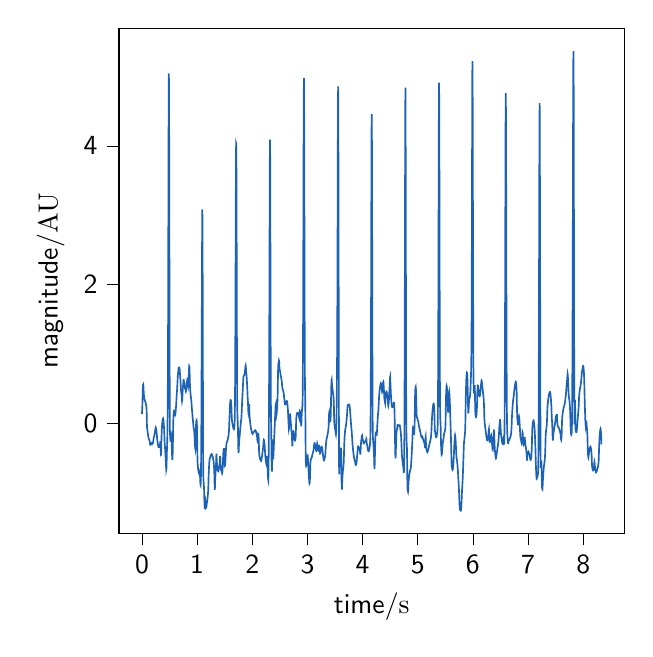
\begin{tikzpicture}
\pgfplotsset{
   every axis/.append style={
		font=\fontsize{10}{10}\sffamily},
	every non boxed x axis/.append style={
		x axis line style={->}
	},
	every non boxed y axis/.append style={
		y axis line style={->}
	},
	every non boxed z axis/.append style={
		z axis line style={->}
	}
}
\begin{axis}[
height=\figH,
tick align=outside,
tick pos=left,
width=\figW,
x grid style={white!69.0196078431373!black},
xlabel={time/$\si{\second}$},
xmin=-0.416499996185303, xmax=8.74649991989136,
xtick style={color=black},
y grid style={white!69.0196078431373!black},
ylabel={magnitude/\si{AU}},
ymin=-1.58700031638145, ymax=5.69556433558464,
ytick style={color=black},
ytick = {0, 2, 4},
yticklabels = {0, 2, 4},
xtick = {0, 1, 2, 3, 4, 5, 6, 7, 8},
xticklabels = {0, 1, 2, 3, 4, 5, 6, 7, 8},
]
\addplot [semithick, tud1b]
table {%
0 0.133536517620087
0.00333333341404796 0.203129768371582
0.00666666682809591 0.250175327062607
0.00999999977648258 0.34033527970314
0.0133333336561918 0.456971526145935
0.0166666675359011 0.522969365119934
0.0199999995529652 0.559824228286743
0.0233333334326744 0.564423024654388
0.0266666673123837 0.5280801653862
0.0299999993294477 0.478881180286407
0.0333333350718021 0.429882884025574
0.0366666652262211 0.392938017845154
0.0399999991059303 0.367589890956879
0.0433333329856396 0.352299928665161
0.0466666668653488 0.345833301544189
0.0500000007450581 0.339366644620895
0.0533333346247673 0.327630966901779
0.0566666685044765 0.321164309978485
0.0599999986588955 0.31747367978096
0.0633333325386047 0.309526413679123
0.0666666701436043 0.296590536832809
0.0700000002980232 0.283657252788544
0.0733333304524422 0.270723968744278
0.0766666680574417 0.257790684700012
0.0799999982118607 0.240163415670395
0.0833333358168602 0.21113620698452
0.0866666659712791 0.115525871515274
0.0900000035762787 -0.019859379157424
0.0933333337306976 -0.0724415257573128
0.0966666638851166 -0.0886769592761993
0.100000001490116 -0.108076885342598
0.103333331644535 -0.127476811408997
0.106666669249535 -0.146876722574234
0.109999999403954 -0.166276663541794
0.113333337008953 -0.184812128543854
0.116666667163372 -0.195684641599655
0.119999997317791 -0.205412238836288
0.123333334922791 -0.218345552682877
0.126666665077209 -0.230891615152359
0.129999995231628 -0.237358272075653
0.133333340287209 -0.241042464971542
0.136666670441628 -0.245022520422935
0.140000000596046 -0.261848419904709
0.143333330750465 -0.281248331069946
0.146666660904884 -0.298343062400818
0.150000005960464 -0.304270714521408
0.153333336114883 -0.299570292234421
0.156666666269302 -0.299001693725586
0.159999996423721 -0.299001693725586
0.16333332657814 -0.299001693725586
0.16666667163372 -0.294778496026993
0.170000001788139 -0.288311868906021
0.173333331942558 -0.28319463133812
0.176666662096977 -0.285741686820984
0.180000007152557 -0.288463652133942
0.183333337306976 -0.293405920267105
0.186666667461395 -0.288463652133942
0.189999997615814 -0.288463652133942
0.193333327770233 -0.288463652133942
0.196666672825813 -0.283998608589172
0.200000002980232 -0.277138322591782
0.203333333134651 -0.26261380314827
0.20666666328907 -0.240424990653992
0.209999993443489 -0.22253143787384
0.213333338499069 -0.209595561027527
0.216666668653488 -0.196662276983261
0.219999998807907 -0.183728992938995
0.223333328962326 -0.17079570889473
0.226666674017906 -0.157862424850464
0.230000004172325 -0.144929140806198
0.233333334326744 -0.131995856761932
0.236666664481163 -0.116028010845184
0.239999994635582 -0.092398464679718
0.243333339691162 -0.0773863792419434
0.246666669845581 -0.0644530951976776
0.25 -0.0566267482936382
0.253333330154419 -0.0641289278864861
0.256666660308838 -0.0770622119307518
0.259999990463257 -0.0908766686916351
0.263333320617676 -0.112352818250656
0.266666680574417 -0.141493231058121
0.270000010728836 -0.16935496032238
0.273333340883255 -0.200490564107895
0.276666671037674 -0.226357132196426
0.280000001192093 -0.249428391456604
0.283333331346512 -0.268832176923752
0.286666661500931 -0.29342395067215
0.28999999165535 -0.306511580944061
0.293333321809769 -0.319444864988327
0.296666651964188 -0.332378149032593
0.300000011920929 -0.3405981361866
0.303333342075348 -0.341153830289841
0.306666672229767 -0.341153830289841
0.310000002384186 -0.341153830289841
0.313333332538605 -0.332681745290756
0.316666662693024 -0.325182139873505
0.319999992847443 -0.318715512752533
0.323333323001862 -0.309688955545425
0.326666653156281 -0.300513207912445
0.330000013113022 -0.284136265516281
0.333333343267441 -0.256849527359009
0.33666667342186 -0.283924013376236
0.340000003576279 -0.367990344762802
0.343333333730698 -0.452056676149368
0.346666663885117 -0.449348837137222
0.349999994039536 -0.329690873622894
0.353333324193954 -0.228163212537766
0.356666654348373 -0.145613491535187
0.360000014305115 -0.0836086124181747
0.363333344459534 -0.0404543541371822
0.366666674613953 -0.00812114495784044
0.370000004768372 0.0206899493932724
0.373333334922791 0.0465565174818039
0.376666665077209 0.0605883710086346
0.379999995231628 0.0716769844293594
0.383333325386047 0.0750987604260445
0.386666655540466 0.0666137859225273
0.389999985694885 0.0478982105851173
0.393333345651627 0.0141962943598628
0.396666675806046 -0.0246035549789667
0.400000005960464 -0.0671673566102982
0.403333336114883 -0.112433858215809
0.406666666269302 -0.18851175904274
0.409999996423721 -0.257755160331726
0.41333332657814 -0.30291485786438
0.416666656732559 -0.341714680194855
0.419999986886978 -0.375658452510834
0.423333346843719 -0.420924961566925
0.426666676998138 -0.466191411018372
0.430000007152557 -0.511466920375824
0.433333337306976 -0.561938166618347
0.436666667461395 -0.615937888622284
0.439999997615814 -0.666618704795837
0.443333327770233 -0.653671264648438
0.446666657924652 -0.565869331359863
0.449999988079071 -0.472941070795059
0.453333348035812 -0.37316158413887
0.456666678190231 -0.29178249835968
0.46000000834465 -0.186658084392548
0.463333338499069 -0.0277397558093071
0.466666668653488 0.271919041872025
0.469999998807907 0.707340002059937
0.473333328962326 1.41428673267365
0.476666659116745 2.4128999710083
0.479999989271164 3.5699770450592
0.483333319425583 4.53656816482544
0.486666679382324 5.04312610626221
0.490000009536743 4.9260048866272
0.493333339691162 4.11327838897705
0.496666669845581 2.79892349243164
0.5 1.39459216594696
0.503333330154419 0.288514643907547
0.506666660308838 -0.107001468539238
0.509999990463257 -0.176394060254097
0.513333320617676 -0.223452478647232
0.516666650772095 -0.248112425208092
0.519999980926514 -0.246847897768021
0.523333311080933 -0.239720061421394
0.526666641235352 -0.226784199476242
0.529999971389771 -0.210793197154999
0.533333361148834 -0.178627207875252
0.536666691303253 -0.192031309008598
0.540000021457672 -0.313074707984924
0.543333351612091 -0.403607666492462
0.54666668176651 -0.482810199260712
0.550000011920929 -0.524103105068207
0.553333342075348 -0.501623511314392
0.556666672229767 -0.435015946626663
0.560000002384186 -0.334451794624329
0.563333332538605 -0.137102797627449
0.566666662693024 0.0112852118909359
0.569999992847443 0.0791714414954185
0.573333323001862 0.134550184011459
0.576666653156281 0.166193887591362
0.579999983310699 0.175158679485321
0.583333313465118 0.168794944882393
0.586666643619537 0.164672091603279
0.589999973773956 0.161130681633949
0.593333303928375 0.154664054512978
0.596666693687439 0.147529780864716
0.600000023841858 0.134593918919563
0.603333353996277 0.127788960933685
0.606666684150696 0.136312529444695
0.610000014305115 0.165624022483826
0.613333344459534 0.199345231056213
0.616666674613953 0.235559463500977
0.620000004768372 0.271675914525986
0.623333334922791 0.3154656291008
0.626666665077209 0.371270209550858
0.629999995231628 0.414428293704987
0.633333325386047 0.453228116035461
0.636666655540466 0.487524390220642
0.639999985694885 0.536961317062378
0.643333315849304 0.588694453239441
0.646666646003723 0.64043790102005
0.649999976158142 0.684118270874023
0.653333306312561 0.712470054626465
0.656666696071625 0.733067631721497
0.660000026226044 0.761284410953522
0.663333356380463 0.790069818496704
0.666666686534882 0.806445479393005
0.670000016689301 0.807492613792419
0.673333346843719 0.80749249458313
0.676666676998138 0.807492554187775
0.680000007152557 0.798956155776978
0.683333337306976 0.7801633477211
0.686666667461395 0.746435701847076
0.689999997615814 0.707635879516602
0.693333327770233 0.672625660896301
0.696666657924652 0.640286147594452
0.699999988079071 0.594663262367249
0.70333331823349 0.54081529378891
0.706666648387909 0.492552876472473
0.709999978542328 0.462773084640503
0.713333308696747 0.442614197731018
0.716666638851166 0.423214286565781
0.720000028610229 0.395304977893829
0.723333358764648 0.352472305297852
0.726666688919067 0.32289707660675
0.730000019073486 0.336124926805496
0.733333349227905 0.388461410999298
0.736666679382324 0.449573516845703
0.740000009536743 0.488765746355057
0.743333339691162 0.527056157588959
0.746666669845581 0.565856039524078
0.75 0.604655861854553
0.753333330154419 0.626357138156891
0.756666660308838 0.627939403057098
0.759999990463257 0.613605260848999
0.763333320617676 0.596803784370422
0.766666650772095 0.587666630744934
0.769999980926514 0.57620370388031
0.773333311080933 0.550885140895844
0.776666641235352 0.525018572807312
0.779999971389771 0.505789697170258
0.783333361148834 0.497372925281525
0.786666691303253 0.490906268358231
0.790000021457672 0.482796907424927
0.793333351612091 0.47270268201828
0.79666668176651 0.462196797132492
0.800000011920929 0.47021096944809
0.803333342075348 0.498344153165817
0.806666672229767 0.532417833805084
0.810000002384186 0.558284401893616
0.813333332538605 0.579392611980438
0.816666662693024 0.60475367307663
0.819999992847443 0.628734350204468
0.823333323001862 0.638883948326111
0.826666653156281 0.634602844715118
0.829999983310699 0.616969168186188
0.833333313465118 0.591102600097656
0.836666643619537 0.562631130218506
0.839999973773956 0.54170298576355
0.843333303928375 0.558778345584869
0.846666693687439 0.627419710159302
0.850000023841858 0.728758275508881
0.853333353996277 0.795830190181732
0.856666684150696 0.825584232807159
0.860000014305115 0.819235861301422
0.863333344459534 0.75443959236145
0.866666674613953 0.650420188903809
0.870000004768372 0.549407064914703
0.873333334922791 0.496800482273102
0.876666665077209 0.463243901729584
0.879999995231628 0.429183095693588
0.883333325386047 0.403316557407379
0.886666655540466 0.38221475481987
0.889999985694885 0.362810969352722
0.893333315849304 0.341518759727478
0.896666646003723 0.309472382068634
0.899999976158142 0.270672529935837
0.903333306312561 0.232088804244995
0.906666696071625 0.19975557923317
0.910000026226044 0.167422384023666
0.913333356380463 0.135082751512527
0.916666686534882 0.102749533951283
0.920000016689301 0.0713528171181679
0.923333346843719 0.0454862453043461
0.926666676998138 0.0196196809411049
0.930000007152557 -0.0107762366533279
0.933333337306976 -0.0426514931023121
0.936666667461395 -0.065206915140152
0.939999997615814 -0.075288288295269
0.943333327770233 -0.0858070403337479
0.946666657924652 -0.103990040719509
0.949999988079071 -0.137462988495827
0.95333331823349 -0.181014746427536
0.956666648387909 -0.236321434378624
0.959999978542328 -0.294521242380142
0.963333308696747 -0.344659209251404
0.966666638851166 -0.359904140233994
0.970000028610229 -0.31236332654953
0.973333358764648 -0.219760566949844
0.976666688919067 -0.0807464122772217
0.980000019073486 -0.0203404873609543
0.983333349227905 0.0196904316544533
0.986666679382324 0.0443966835737228
0.990000009536743 0.0487536564469337
0.993333339691162 0.0220200680196285
0.996666669845581 -0.0232014004141092
1 -0.151502564549446
1.00333333015442 -0.390859633684158
1.00666666030884 -0.524944365024567
1.00999999046326 -0.584633767604828
1.01333332061768 -0.621317505836487
1.01666665077209 -0.647184073925018
1.01999998092651 -0.667794525623322
1.02333331108093 -0.681925415992737
1.02666664123535 -0.701325356960297
1.02999997138977 -0.717145264148712
1.03333330154419 -0.725300967693329
1.03666663169861 -0.725084841251373
1.03999996185303 -0.718618154525757
1.04333329200745 -0.712151527404785
1.04666662216187 -0.701384484767914
1.04999995231628 -0.691885888576508
1.0533332824707 -0.773099005222321
1.05666661262512 -0.838983654975891
1.05999994277954 -0.881902515888214
1.06333339214325 -0.889131963253021
1.06666672229767 -0.846125662326813
1.07000005245209 -0.721292555332184
1.07333338260651 -0.421156495809555
1.07666671276093 0.0492952167987823
1.08000004291534 0.6380735039711
1.08333337306976 1.2884167432785
1.08666670322418 1.98175096511841
1.0900000333786 2.66056156158447
1.09333336353302 3.08334255218506
1.09666669368744 2.98740530014038
1.10000002384186 2.3139808177948
1.10333335399628 1.18177819252014
1.1066666841507 0.0471585392951965
1.11000001430511 -0.656209349632263
1.11333334445953 -0.795220971107483
1.11666667461395 -0.830911636352539
1.12000000476837 -0.867551624774933
1.12333333492279 -0.906822323799133
1.12666666507721 -0.968586683273315
1.12999999523163 -1.07610893249512
1.13333332538605 -1.16836297512054
1.13666665554047 -1.21938741207123
1.13999998569489 -1.22157037258148
1.1433333158493 -1.18708372116089
1.14666664600372 -1.14828395843506
1.14999997615814 -1.1322273015976
1.15333330631256 -1.15976107120514
1.15666663646698 -1.18395662307739
1.1599999666214 -1.20048272609711
1.16333329677582 -1.21341598033905
1.16666662693024 -1.21054220199585
1.16999995708466 -1.18994474411011
1.17333328723907 -1.16647338867188
1.17666661739349 -1.14707338809967
1.17999994754791 -1.13246142864227
1.18333327770233 -1.11353874206543
1.18666660785675 -1.09222078323364
1.19000005722046 -1.06635415554047
1.19333338737488 -1.04048764705658
1.1966667175293 -1.0141373872757
1.20000004768372 -0.972458600997925
1.20333337783813 -0.902246654033661
1.20666670799255 -0.801411032676697
1.21000003814697 -0.718079209327698
1.21333336830139 -0.665404319763184
1.21666669845581 -0.615831077098846
1.22000002861023 -0.5705646276474
1.22333335876465 -0.538963377475739
1.22666668891907 -0.519333183765411
1.23000001907349 -0.506397306919098
1.23333334922791 -0.496344208717346
1.23666667938232 -0.489877581596375
1.24000000953674 -0.478135466575623
1.24333333969116 -0.466406255960464
1.24666666984558 -0.457537949085236
1.25 -0.451803267002106
1.25333333015442 -0.451803237199783
1.25666666030884 -0.446534216403961
1.25999999046326 -0.444609820842743
1.26333332061768 -0.441265225410461
1.26666665077209 -0.445584863424301
1.26999998092651 -0.452051520347595
1.27333331108093 -0.458518147468567
1.27666664123535 -0.462341278791428
1.27999997138977 -0.470026105642319
1.28333330154419 -0.482959389686584
1.28666663169861 -0.495892703533173
1.28999996185303 -0.508826017379761
1.29333329200745 -0.521759271621704
1.29666662216187 -0.534692585468292
1.29999995231628 -0.559640645980835
1.3033332824707 -0.593662858009338
1.30666661262512 -0.632462739944458
1.30999994277954 -0.679431080818176
1.31333339214325 -0.757650911808014
1.31666672229767 -0.874464631080627
1.32000005245209 -0.955365240573883
1.32333338260651 -0.922676980495453
1.32666671276093 -0.827136099338531
1.33000004291534 -0.768080830574036
1.33333337306976 -0.722814321517944
1.33666670322418 -0.683804750442505
1.3400000333786 -0.651471555233002
1.34333336353302 -0.574439167976379
1.34666669368744 -0.486153483390808
1.35000002384186 -0.43589586019516
1.35333335399628 -0.477921932935715
1.3566666841507 -0.549689173698425
1.36000001430511 -0.57786613702774
1.36333334445953 -0.610199272632599
1.36666667461395 -0.635791897773743
1.37000000476837 -0.655191779136658
1.37333333492279 -0.668828725814819
1.37666666507721 -0.680066585540771
1.37999999523163 -0.686533212661743
1.38333332538605 -0.68890917301178
1.38666665554047 -0.683601558208466
1.38999998569489 -0.670668244361877
1.3933333158493 -0.655320405960083
1.39666664600372 -0.639530122280121
1.39999997615814 -0.626596808433533
1.40333330631256 -0.607654809951782
1.40666663646698 -0.588254928588867
1.4099999666214 -0.562585175037384
1.41333329677582 -0.508589267730713
1.41666662693024 -0.468915969133377
1.41999995708466 -0.508543014526367
1.42333328723907 -0.56259161233902
1.42666661739349 -0.605246782302856
1.42999994754791 -0.645460307598114
1.43333327770233 -0.668814599514008
1.43666660785675 -0.675281167030334
1.44000005722046 -0.681747913360596
1.44333338737488 -0.6927889585495
1.4466667175293 -0.705220520496368
1.45000004768372 -0.713389039039612
1.45333337783813 -0.720523297786713
1.45666670799255 -0.712329030036926
1.46000003814697 -0.678216755390167
1.46333336830139 -0.636970221996307
1.46666669845581 -0.582816123962402
1.47000002861023 -0.502885460853577
1.47333335876465 -0.434790879487991
1.47666668891907 -0.406666696071625
1.48000001907349 -0.382743835449219
1.48333334922791 -0.366485267877579
1.48666667938232 -0.366568863391876
1.49000000953674 -0.412594348192215
1.49333333969116 -0.477866619825363
1.49666666984558 -0.5284703373909
1.5 -0.578946650028229
1.50333333015442 -0.609035134315491
1.50666666030884 -0.605922102928162
1.50999999046326 -0.575684368610382
1.51333332061768 -0.530118227005005
1.51666665077209 -0.482965856790543
1.51999998092651 -0.421372622251511
1.52333331108093 -0.371347784996033
1.52666664123535 -0.328987240791321
1.52999997138977 -0.298394501209259
1.53333330154419 -0.283162474632263
1.53666663169861 -0.276695817708969
1.53999996185303 -0.270229190587997
1.54333329200745 -0.263761252164841
1.54666662216187 -0.252470672130585
1.54999995231628 -0.245558947324753
1.5533332824707 -0.237142160534859
1.55666661262512 -0.224208876490593
1.55999994277954 -0.211275577545166
1.56333339214325 -0.198616296052933
1.56666672229767 -0.189202561974525
1.57000005245209 -0.16713210940361
1.57333338260651 -0.141265526413918
1.57666671276093 -0.110333196818829
1.58000004291534 -0.0647759735584259
1.58333337306976 0.0149063775315881
1.58666670322418 0.0792602002620697
1.5900000333786 0.151221677660942
1.59333336353302 0.232037335634232
1.59666669368744 0.27862623333931
1.60000002384186 0.30513471364975
1.60333335399628 0.324534624814987
1.6066666841507 0.338549792766571
1.61000001430511 0.337313592433929
1.61333334445953 0.328413069248199
1.61666667461395 0.304578989744186
1.62000000476837 0.267415404319763
1.62333333492279 0.205977812409401
1.62666666507721 0.116804540157318
1.62999999523163 0.061442531645298
1.63333332538605 0.0313463360071182
1.63666665554047 0.0113096535205841
1.63999998569489 -0.00162620283663273
1.6433333158493 -0.0172364469617605
1.64666664600372 -0.0327617898583412
1.64999997615814 -0.045695073902607
1.65333330631256 -0.0533593371510506
1.65666663646698 -0.0662926211953163
1.6599999666214 -0.0758298560976982
1.66333329677582 -0.0777028277516365
1.66666662693024 -0.0824482962489128
1.66999995708466 -0.0759816467761993
1.67333328723907 -0.0636774078011513
1.67666661739349 -0.0360446386039257
1.67999994754791 0.00718679931014776
1.68333327770233 0.109892815351486
1.68666660785675 0.351965457201004
1.69000005722046 0.774827420711517
1.69333338737488 1.39525592327118
1.6966667175293 2.20020031929016
1.70000004768372 3.03670740127563
1.70333337783813 3.7148699760437
1.70666670799255 4.03987169265747
1.71000003814697 4.03044128417969
1.71333336830139 3.54675149917603
1.71666669845581 2.6730523109436
1.72000002861023 1.63967490196228
1.72333335876465 0.702420949935913
1.72666668891907 0.261685878038406
1.73000001907349 0.130739912390709
1.73333334922791 0.0636859759688377
1.73666667938232 0.0211453288793564
1.74000000953674 -0.0656674429774284
1.74333333969116 -0.235083937644958
1.74666666984558 -0.363956242799759
1.75 -0.427973031997681
1.75333333015442 -0.403816074132919
1.75666666030884 -0.336430251598358
1.75999999046326 -0.287134826183319
1.76333332061768 -0.245513930916786
1.76666665077209 -0.216400533914566
1.76999998092651 -0.190533950924873
1.77333331108093 -0.162697941064835
1.77666664123535 -0.127197653055191
1.77999997138977 -0.0927625149488449
1.78333330154419 -0.06599161028862
1.78666663169861 -0.0386276915669441
1.78999996185303 -0.00898430682718754
1.79333329200745 0.0168822593986988
1.79666662216187 0.0376637615263462
1.79999995231628 0.0580773539841175
1.8033332824707 0.0883665010333061
1.80666661262512 0.137393087148666
1.80999994277954 0.200212255120277
1.81333339214325 0.274880290031433
1.81666672229767 0.329611986875534
1.82000005245209 0.374878525733948
1.82333338260651 0.424274265766144
1.82666671276093 0.481276422739029
1.83000004291534 0.53300952911377
1.83333337306976 0.584752976894379
1.83666670322418 0.636486113071442
1.8400000333786 0.673670291900635
1.84333336353302 0.681814312934875
1.84666669368744 0.688280940055847
1.85000002384186 0.691574096679688
1.85333335399628 0.695945262908936
1.8566666841507 0.702714204788208
1.86000001430511 0.715647459030151
1.86333334445953 0.731276988983154
1.86666667461395 0.750676870346069
1.87000000476837 0.770076870918274
1.87333333492279 0.801034927368164
1.87666666507721 0.826901435852051
1.87999999523163 0.835691332817078
1.88333332538605 0.81538063287735
1.88666665554047 0.772621333599091
1.88999998569489 0.737302422523499
1.8933333158493 0.711435854434967
1.89666664600372 0.68143355846405
1.89999997615814 0.643702685832977
1.90333330631256 0.597174286842346
1.90666663646698 0.547891736030579
1.9099999666214 0.498966753482819
1.91333329677582 0.432665348052979
1.91666662693024 0.37072479724884
1.91999995708466 0.329942613840103
1.92333328723907 0.268776416778564
1.92666661739349 0.191176697611809
1.92999994754791 0.142058789730072
1.93333327770233 0.130796521902084
1.93666660785675 0.194401666522026
1.94000005722046 0.257734090089798
1.94333338737488 0.259856641292572
1.9466667175293 0.171240359544754
1.95000004768372 0.119713053107262
1.95333337783813 0.0809132009744644
1.95666670799255 0.0513470023870468
1.96000003814697 0.0307494569569826
1.96333336830139 0.00662979623302817
1.96666669845581 -0.0157146565616131
1.97000002861023 -0.0415812246501446
1.97333335876465 -0.056768249720335
1.97666668891907 -0.0697015374898911
1.98000001907349 -0.0826373919844627
1.98333334922791 -0.0955706760287285
1.98666667938232 -0.108503960072994
1.99000000953674 -0.125915139913559
1.99333333969116 -0.132381767034531
1.99666666984558 -0.138848423957825
2 -0.145315065979958
2.00333333015442 -0.14651395380497
2.00666666030884 -0.149957612156868
2.00999999046326 -0.143490970134735
2.01333332061768 -0.137024328112602
2.01666665077209 -0.130557686090469
2.01999998092651 -0.125124022364616
2.02333331108093 -0.125124022364616
2.02666664123535 -0.121694520115852
2.02999997138977 -0.115227878093719
2.03333330154419 -0.114585973322392
2.03666663169861 -0.114585965871811
2.03999996185303 -0.114585973322392
2.04333329200745 -0.110437393188477
2.04666662216187 -0.103970743715763
2.04999995231628 -0.0987789109349251
2.0533332824707 -0.0963051989674568
2.05666661262512 -0.0971812233328819
2.05999994277954 -0.103647865355015
2.06333327293396 -0.110114507377148
2.06666660308838 -0.11857633292675
2.0699999332428 -0.128316819667816
2.07333326339722 -0.139173865318298
2.07666659355164 -0.152109727263451
2.07999992370605 -0.165043026208878
2.08333325386047 -0.177976295351982
2.08666658401489 -0.194822758436203
2.08999991416931 -0.224444270133972
2.09333324432373 -0.253659307956696
2.09666657447815 -0.259881526231766
2.09999990463257 -0.246541738510132
2.10333323478699 -0.222508266568184
2.10666656494141 -0.194955259561539
2.10999989509583 -0.156727835536003
2.11333322525024 -0.160987049341202
2.11666655540466 -0.222405359148979
2.11999988555908 -0.310877561569214
2.1233332157135 -0.40666925907135
2.1266667842865 -0.453974664211273
2.13000011444092 -0.469696819782257
2.13333344459534 -0.482630103826523
2.13666677474976 -0.495563387870789
2.14000010490417 -0.508496701717377
2.14333343505859 -0.518230736255646
2.14666676521301 -0.520300507545471
2.15000009536743 -0.525569558143616
2.15333342552185 -0.528618276119232
2.15666675567627 -0.538829565048218
2.16000008583069 -0.54137659072876
2.16333341598511 -0.536259353160858
2.16666674613953 -0.522432088851929
2.17000007629395 -0.503032088279724
2.17333340644836 -0.487070679664612
2.17666673660278 -0.469497442245483
2.1800000667572 -0.450097501277924
2.18333339691162 -0.430697560310364
2.18666672706604 -0.408333837985992
2.19000005722046 -0.386628717184067
2.19333338737488 -0.367318838834763
2.1966667175293 -0.350516140460968
2.20000004768372 -0.318182945251465
2.20333337783813 -0.28216552734375
2.20666670799255 -0.248247489333153
2.21000003814697 -0.23577344417572
2.21333336830139 -0.239789515733719
2.21666669845581 -0.259134143590927
2.22000002861023 -0.285005867481232
2.22333335876465 -0.311205595731735
2.22666668891907 -0.345069587230682
2.23000001907349 -0.389326274394989
2.23333334922791 -0.437133342027664
2.23666667938232 -0.477276176214218
2.24000000953674 -0.497112184762955
2.24333333969116 -0.516512095928192
2.24666666984558 -0.535915911197662
2.25 -0.559962272644043
2.25333333015442 -0.584678769111633
2.25666666030884 -0.592294156551361
2.25999999046326 -0.576916754245758
2.26333332061768 -0.546882331371307
2.26666665077209 -0.50899064540863
2.26999998092651 -0.468905687332153
2.27333331108093 -0.510274469852448
2.27666664123535 -0.614655315876007
2.27999997138977 -0.719700038433075
2.28333330154419 -0.762307584285736
2.28666663169861 -0.801107466220856
2.28999996185303 -0.814210534095764
2.29333329200745 -0.748342633247375
2.29666662216187 -0.532896757125854
2.29999995231628 -0.14770644903183
2.3033332824707 0.355182707309723
2.30666661262512 0.996429860591888
2.30999994277954 1.81148278713226
2.31333327293396 2.76406669616699
2.31666660308838 3.64065599441528
2.3199999332428 4.09018182754517
2.32333326339722 4.05903100967407
2.32666659355164 3.31859230995178
2.32999992370605 2.16978907585144
2.33333325386047 1.09109091758728
2.33666658401489 0.369671165943146
2.33999991416931 0.057130578905344
2.34333324432373 -0.0917140990495682
2.34666657447815 -0.332171022891998
2.34999990463257 -0.543676614761353
2.35333323478699 -0.656574666500092
2.35666656494141 -0.694342851638794
2.35999989509583 -0.543183922767639
2.36333322525024 -0.361970067024231
2.36666655540466 -0.270634412765503
2.36999988555908 -0.230425953865051
2.3733332157135 -0.32588192820549
2.3766667842865 -0.402708500623703
2.38000011444092 -0.453030437231064
2.38333344459534 -0.462341278791428
2.38666677474976 -0.4095379114151
2.39000010490417 -0.347122669219971
2.39333343505859 -0.285461246967316
2.39666676521301 -0.225454092025757
2.40000009536743 -0.161397412419319
2.40333342552185 -0.0985164940357208
2.40666675567627 -0.0373335890471935
2.41000008583069 0.0273328274488449
2.41333341598511 0.091999240219593
2.41666674613953 0.155370265245438
2.42000007629395 0.213570043444633
2.42333340644836 0.264362812042236
2.42666673660278 0.275321513414383
2.4300000667572 0.243998125195503
2.43333339691162 0.205198273062706
2.43666672706604 0.163173466920853
2.44000005722046 0.131169572472572
2.44333338737488 0.146415770053864
2.4466667175293 0.195048719644547
2.45000004768372 0.231100857257843
2.45333337783813 0.271324723958969
2.45666670799255 0.321734189987183
2.46000003814697 0.415885776281357
2.46333336830139 0.582811832427979
2.46666669845581 0.738192617893219
2.47000002861023 0.82659786939621
2.47333335876465 0.866640388965607
2.47666668891907 0.877781748771667
2.48000001907349 0.887237906455994
2.48333334922791 0.908545613288879
2.48666667938232 0.900930166244507
2.49000000953674 0.831218540668488
2.49333333969116 0.797443330287933
2.49666666984558 0.778996586799622
2.5 0.766063332557678
2.50333333015442 0.75313001871109
2.50666666030884 0.740196764469147
2.50999999046326 0.72403210401535
2.51333332061768 0.70462828874588
2.51666665077209 0.685587346553802
2.51999998092651 0.672654032707214
2.52333331108093 0.659720718860626
2.52666664123535 0.646787464618683
2.52999997138977 0.628704786300659
2.53333330154419 0.614573895931244
2.53666663169861 0.590616285800934
2.53999996185303 0.554808616638184
2.54333329200745 0.525353014469147
2.54666662216187 0.511225998401642
2.54999995231628 0.498292684555054
2.5533332824707 0.488355398178101
2.55666661262512 0.477695137262344
2.55999994277954 0.470028281211853
2.56333327293396 0.45709502696991
2.56666660308838 0.446680456399918
2.5699999332428 0.432781100273132
2.57333326339722 0.408467233181
2.57666659355164 0.378174245357513
2.57999992370605 0.358774304389954
2.58333325386047 0.336131393909454
2.58666658401489 0.305828064680099
2.58999991416931 0.285128891468048
2.59333324432373 0.273758560419083
2.59666657447815 0.272813081741333
2.59999990463257 0.275321513414383
2.60333323478699 0.280477315187454
2.60666656494141 0.286943972110748
2.60999989509583 0.293411910533905
2.61333322525024 0.303359478712082
2.61666655540466 0.311614215373993
2.61999988555908 0.318080872297287
2.6233332157135 0.322742700576782
2.6266667842865 0.322742700576782
2.63000011444092 0.318542659282684
2.63333344459534 0.306545853614807
2.63666677474976 0.284490823745728
2.64000010490417 0.252157628536224
2.64333343505859 0.223547220230103
2.64666676521301 0.187839835882187
2.65000009536743 0.125416874885559
2.65333342552185 0.0651704594492912
2.65666675567627 0.00698226504027843
2.66000008583069 -0.0491940341889858
2.66333341598511 -0.0826000869274139
2.66666674613953 -0.0682865083217621
2.67000007629395 -0.0211856383830309
2.67333340644836 0.0251202490180731
2.67666673660278 0.0639200955629349
2.6800000667572 0.101635530591011
2.68333339691162 0.127099454402924
2.68666672706604 0.129570603370667
2.69000005722046 0.104363948106766
2.69333338737488 0.0661481097340584
2.6966667175293 0.029159490019083
2.70000004768372 -0.00618256675079465
2.70333337783813 -0.0449824184179306
2.70666670799255 -0.0782482475042343
2.71000003814697 -0.102780848741531
2.71333336830139 -0.124712370336056
2.71666669845581 -0.150578930974007
2.72000002861023 -0.206006556749344
2.72333335876465 -0.289182752370834
2.72666668891907 -0.330343097448349
2.73000001907349 -0.29764324426651
2.73333334922791 -0.218442022800446
2.73666667938232 -0.175545036792755
2.74000000953674 -0.141472637653351
2.74333333969116 -0.124846160411835
2.74666666984558 -0.115883931517601
2.75 -0.119754657149315
2.75333333015442 -0.133688732981682
2.75666666030884 -0.15308865904808
2.75999999046326 -0.168994784355164
2.76333332061768 -0.186619490385056
2.76666665077209 -0.206639468669891
2.76999998092651 -0.230688378214836
2.77333331108093 -0.247073024511337
2.77666664123535 -0.247366324067116
2.77999997138977 -0.240614086389542
2.78333330154419 -0.219873756170273
2.78666663169861 -0.18893113732338
2.78999996185303 -0.135188668966293
2.79333329200745 -0.016229210421443
2.79666662216187 0.0636010766029358
2.79999995231628 0.0938799306750298
2.8033332824707 0.116484224796295
2.80666661262512 0.135888025164604
2.80999994277954 0.143979355692863
2.81333327293396 0.15044729411602
2.81666660308838 0.154134064912796
2.8199999332428 0.154134064912796
2.82333326339722 0.154134064912796
2.82666659355164 0.154134064912796
2.82999992370605 0.154134064912796
2.83333325386047 0.150635108351707
2.83666658401489 0.139469310641289
2.83999991416931 0.121892176568508
2.84333324432373 0.113602742552757
2.84666657447815 0.100666880607605
2.84999990463257 0.0792975127696991
2.85333323478699 0.0707250609993935
2.85666656494141 0.109517194330692
2.85999989509583 0.148324757814407
2.86333322525024 0.17590220272541
2.86666655540466 0.170599728822708
2.86999988555908 0.127840414643288
2.8733332157135 0.0890482813119888
2.8766667842865 0.0535055510699749
2.88000011444092 0.0256399475038052
2.88333344459534 0.00386407482437789
2.88666677474976 -0.0398214533925056
2.89000010490417 -0.0173149164766073
2.89333343505859 0.0742162987589836
2.89666676521301 0.132358193397522
2.90000009536743 0.176609724760056
2.90333342552185 0.210786312818527
2.90666675567627 0.236658036708832
2.91000008583069 0.262529730796814
2.91333341598511 0.385574758052826
2.91666674613953 0.696555018424988
2.92000007629395 1.22622537612915
2.92333340644836 2.01673793792725
2.92666673660278 3.0247209072113
2.9300000667572 4.0502758026123
2.93333339691162 4.77422046661377
2.93666672706604 4.97751522064209
2.94000005722046 4.64907884597778
2.94333338737488 3.66218996047974
2.9466667175293 2.4462194442749
2.95000004768372 1.36807203292847
2.95333337783813 0.727639079093933
2.95666670799255 0.50252228975296
2.96000003814697 0.321682751178741
2.96333336830139 0.0320769958198071
2.96666669845581 -0.335488617420197
2.97000002861023 -0.544571995735168
2.97333335876465 -0.593264102935791
2.97666668891907 -0.614504814147949
2.98000001907349 -0.609876394271851
2.98333334922791 -0.581051170825958
2.98666667938232 -0.544083178043365
2.99000000953674 -0.520058691501617
2.99333333969116 -0.49761900305748
2.99666666984558 -0.475989788770676
3 -0.462179183959961
3.00333333015442 -0.459789097309113
3.00666666030884 -0.47783961892128
3.00999999046326 -0.51498007774353
3.01333332061768 -0.560237526893616
3.01666665077209 -0.613429367542267
3.01999998092651 -0.678082942962646
3.02333331108093 -0.732929170131683
3.02666664123535 -0.773712635040283
3.02999997138977 -0.812520205974579
3.03333330154419 -0.848122119903564
3.03666663169861 -0.865586042404175
3.03999996185303 -0.86005973815918
3.04333329200745 -0.826351404190063
3.04666662216187 -0.770259976387024
3.04999995231628 -0.669469356536865
3.0533332824707 -0.57292902469635
3.05666661262512 -0.543028295040131
3.05999994277954 -0.529547035694122
3.06333327293396 -0.518455862998962
3.06666660308838 -0.511990487575531
3.0699999332428 -0.505522608757019
3.07333326339722 -0.499057203531265
3.07666659355164 -0.492589235305786
3.07999992370605 -0.483556270599365
3.08333325386047 -0.470625579357147
3.08666658401489 -0.457689702510834
3.08999991416931 -0.444759011268616
3.09333324432373 -0.43390965461731
3.09666657447815 -0.424161493778229
3.09999990463257 -0.415707379579544
3.10333323478699 -0.408827811479568
3.10666656494141 -0.397505074739456
3.10999989509583 -0.385423392057419
3.11333322525024 -0.366027325391769
3.11666655540466 -0.341421395540237
3.11999988555908 -0.315559983253479
3.1233332157135 -0.294344991445541
3.1266667842865 -0.284938961267471
3.13000011444092 -0.283194661140442
3.13333344459534 -0.289117127656937
3.13666677474976 -0.29743230342865
3.14000010490417 -0.307319462299347
3.14333343505859 -0.318029880523682
3.14666676521301 -0.331315606832504
3.15000009536743 -0.355805724859238
3.15333342552185 -0.375209510326385
3.15666675567627 -0.390844196081161
3.16000008583069 -0.393844038248062
3.16333341598511 -0.385889053344727
3.16666674613953 -0.366492986679077
3.17000007629395 -0.343798637390137
3.17333340644836 -0.308963447809219
3.17666673660278 -0.288880437612534
3.1800000667572 -0.298579752445221
3.18333339691162 -0.31797581911087
3.18666672706604 -0.337379604578018
3.19000005722046 -0.356775641441345
3.19333338737488 -0.38031131029129
3.1966667175293 -0.38857501745224
3.20000004768372 -0.385042607784271
3.20333337783813 -0.378574699163437
3.20666670799255 -0.366181671619415
3.21000003814697 -0.347673237323761
3.21333336830139 -0.309238731861115
3.21666669845581 -0.332007676362991
3.22000002861023 -0.373488336801529
3.22333335876465 -0.39798104763031
3.22666668891907 -0.417384833097458
3.23000001907349 -0.433006644248962
3.23333334922791 -0.431023061275482
3.23666667938232 -0.41221871972084
3.24000000953674 -0.392814934253693
3.24333333969116 -0.380010306835175
3.24666666984558 -0.369047731161118
3.25 -0.361380904912949
3.25333333015442 -0.348450183868408
3.25666666030884 -0.338334083557129
3.25999999046326 -0.335884839296341
3.26333332061768 -0.341099798679352
3.26666665077209 -0.355118811130524
3.26999998092651 -0.374522566795349
3.27333331108093 -0.393926382064819
3.27666664123535 -0.418058902025223
3.27999997138977 -0.43866154551506
3.28333330154419 -0.462660312652588
3.28666663169861 -0.482064098119736
3.28999996185303 -0.501460194587708
3.29333329200745 -0.520676136016846
3.29666662216187 -0.532222747802734
3.29999995231628 -0.533524513244629
3.3033332824707 -0.527056634426117
3.30666661262512 -0.515612959861755
3.30999994277954 -0.507946074008942
3.31333327293396 -0.497119903564453
3.31666660308838 -0.487348556518555
3.3199999332428 -0.469918072223663
3.32333326339722 -0.449654996395111
3.32666659355164 -0.412429690361023
3.32999992370605 -0.366356611251831
3.33333325386047 -0.32754909992218
3.33666658401489 -0.293977081775665
3.33999991416931 -0.262787461280823
3.34333324432373 -0.239272400736809
3.34666657447815 -0.22341388463974
3.34999990463257 -0.215222209692001
3.35333323478699 -0.202816337347031
3.35666656494141 -0.18988049030304
3.35999989509583 -0.176949769258499
3.36333322525024 -0.164013907313347
3.36666655540466 -0.151083201169968
3.36999988555908 -0.138147339224815
3.3733332157135 -0.122620709240437
3.3766667842865 -0.0994375348091125
3.38000011444092 -0.0785518363118172
3.38333344459534 -0.0458777397871017
3.38666677474976 0.0077155027538538
3.39000010490417 0.111616566777229
3.39333343505859 0.157879993319511
3.39666676521301 0.170815855264664
3.40000009536743 0.178845450282097
3.40333342552185 0.14971661567688
3.40666675567627 0.0995863229036331
3.41000008583069 0.0647665411233902
3.41333341598511 0.03706044703722
3.41666674613953 0.0400088354945183
3.42000007629395 0.0771775469183922
3.42333340644836 0.147897690534592
3.42666673660278 0.280569970607758
3.4300000667572 0.45848947763443
3.43333339691162 0.559858918190002
3.43666672706604 0.616089224815369
3.44000005722046 0.627141833305359
3.44333338737488 0.586934685707092
3.4466667175293 0.546869039535522
3.45000004768372 0.522119045257568
3.45333337783813 0.502722978591919
3.45666670799255 0.483319222927094
3.46000003814697 0.461805760860443
3.46333336830139 0.435934036970139
3.46666669845581 0.414577543735504
3.47000002861023 0.395181477069855
3.47333335876465 0.37249481678009
3.47666668891907 0.331654757261276
3.48000001907349 0.24358132481575
3.48333334922791 0.0813402831554413
3.48666667938232 0.0165941100567579
3.49000000953674 -0.0133734419941902
3.49333333969116 -0.0392451547086239
3.49666666984558 -0.0603598281741142
3.5 -0.0783871859312057
3.50333333015442 -0.0867383778095245
3.50666666030884 -0.0996690839529037
3.50999999046326 -0.11688344925642
3.51333332061768 -0.141548544168472
3.51666665077209 -0.155333399772644
3.51999998092651 -0.130640015006065
3.52333331108093 -0.0675172582268715
3.52666664123535 0.0486198738217354
3.52999997138977 0.231769770383835
3.53333330154419 0.524859070777893
3.53666663169861 0.868410468101501
3.53999996185303 1.32491660118103
3.54333329200745 1.99102580547333
3.54666662216187 2.90489196777344
3.54999995231628 3.89190149307251
3.5533332824707 4.66042757034302
3.55666661262512 4.85897254943848
3.55999994277954 4.48689985275269
3.56333327293396 3.27751040458679
3.56666660308838 1.71633172035217
3.5699999332428 0.268372476100922
3.57333326339722 -0.620097994804382
3.57666659355164 -0.734745562076569
3.57999992370605 -0.555248975753784
3.58333325386047 -0.349980980157852
3.58666658401489 -0.424887031316757
3.58999991416931 -0.561531662940979
3.59333324432373 -0.630949914455414
3.59666657447815 -0.562411546707153
3.59999990463257 -0.461047172546387
3.60333323478699 -0.370565682649612
3.60666656494141 -0.348666310310364
3.60999989509583 -0.414107143878937
3.61333322525024 -0.549938797950745
3.61666655540466 -0.752073109149933
3.61999988555908 -0.885946869850159
3.6233332157135 -0.953656852245331
3.6266667842865 -0.93172150850296
3.63000011444092 -0.842058122158051
3.63333344459534 -0.786059319972992
3.63666677474976 -0.745533108711243
3.64000010490417 -0.716777324676514
3.64333343505859 -0.686135768890381
3.64666676521301 -0.660472393035889
3.65000009536743 -0.639172494411469
3.65333342552185 -0.610218584537506
3.65666675567627 -0.577878952026367
3.66000008583069 -0.517020225524902
3.66333341598511 -0.415748536586761
3.66666674613953 -0.315024852752686
3.67000007629395 -0.248879104852676
3.67333340644836 -0.200691223144531
3.67666673660278 -0.161641806364059
3.6800000667572 -0.127110183238983
3.68333339691162 -0.101248770952225
3.68666672706604 -0.0799102634191513
3.69000005722046 -0.0710445120930672
3.69333338737488 -0.0533078834414482
3.6966667175293 -0.0375136882066727
3.70000004768372 -0.018117617815733
3.70333337783813 0.00128616578876972
3.70666670799255 0.0271321497857571
3.71000003814697 0.0553836673498154
3.71333336830139 0.0877233073115349
3.71666669845581 0.120050072669983
3.72000002861023 0.154504537582397
3.72333335876465 0.204326093196869
3.72666668891907 0.246501415967941
3.73000001907349 0.263810962438583
3.73333334922791 0.264783471822739
3.73666667938232 0.264783471822739
3.74000000953674 0.267405122518539
3.74333333969116 0.270052492618561
3.74666666984558 0.275069385766983
3.75 0.275321513414383
3.75333333015442 0.273178398609161
3.75666666030884 0.270052492618561
3.75999999046326 0.270052492618561
3.76333332061768 0.258109718561172
3.76666665077209 0.238705962896347
3.76999998092651 0.213582903146744
3.77333331108093 0.181243270635605
3.77666664123535 0.148916497826576
3.77999997138977 0.114199616014957
3.78333330154419 0.0713116452097893
3.78666663169861 0.032519519329071
3.78999996185303 -0.00150528270751238
3.79333329200745 -0.0338320583105087
3.79666662216187 -0.0642627105116844
3.79999995231628 -0.0932294577360153
3.8033332824707 -0.125569105148315
3.80666661262512 -0.163411885499954
3.80999994277954 -0.202204018831253
3.81333327293396 -0.243640959262848
3.81666660308838 -0.288898438215256
3.8199999332428 -0.324124723672867
3.82333326339722 -0.350230544805527
3.82666659355164 -0.376102268695831
3.82999992370605 -0.401973962783813
3.83333325386047 -0.42328929901123
3.83666658401489 -0.4479621052742
3.83999991416931 -0.46735817193985
3.84333324432373 -0.483890771865845
3.84666657447815 -0.500889003276825
3.84999990463257 -0.515026390552521
3.85333323478699 -0.521494269371033
3.85666656494141 -0.527962207794189
3.85999989509583 -0.534430146217346
3.86333322525024 -0.545683443546295
3.86666655540466 -0.564606070518494
3.86999988555908 -0.584002137184143
3.8733332157135 -0.59717983007431
3.8766667842865 -0.599335789680481
3.88000011444092 -0.594066798686981
3.88333344459534 -0.592628598213196
3.88666677474976 -0.583528757095337
3.89000010490417 -0.566759467124939
3.89333343505859 -0.537303924560547
3.89666676521301 -0.504964232444763
3.90000009536743 -0.474793434143066
3.90333342552185 -0.448921740055084
3.90666675567627 -0.423050045967102
3.91000008583069 -0.38568839430809
3.91333341598511 -0.35024082660675
3.91666674613953 -0.330132126808167
3.92000007629395 -0.329422056674957
3.92333340644836 -0.341156423091888
3.92666673660278 -0.347624331712723
3.9300000667572 -0.351691871881485
3.93333339691162 -0.351691871881485
3.93666672706604 -0.356487512588501
3.94000005722046 -0.368944823741913
3.94333338737488 -0.379958838224411
3.9466667175293 -0.38642418384552
3.95000004768372 -0.392892122268677
3.95333337783813 -0.405123025178909
3.95666670799255 -0.428849041461945
3.96000003814697 -0.449160993099213
3.96333336830139 -0.404310017824173
3.96666669845581 -0.3432377576828
3.97000002861023 -0.293212980031967
3.97333335876465 -0.258732795715332
3.97666668891907 -0.239586278796196
3.98000001907349 -0.226655572652817
3.98333334922791 -0.206984221935272
3.98666667938232 -0.178027749061584
3.99000000953674 -0.173044323921204
3.99333333969116 -0.194135829806328
3.99666666984558 -0.209448918700218
4 -0.221175581216812
4.003333568573 -0.230046465992928
4.00666666030884 -0.24298232793808
4.01000022888184 -0.251112252473831
4.01333332061768 -0.263579875230789
4.01666688919067 -0.27651059627533
4.01999998092651 -0.28632053732872
4.02333354949951 -0.288463652133942
4.02666664123535 -0.28269037604332
4.03000020980835 -0.271205544471741
4.03333330154419 -0.264740198850632
4.03666687011719 -0.262118548154831
4.03999996185303 -0.262118548154831
4.04333353042603 -0.262118548154831
4.04666662216187 -0.259949713945389
4.05000019073486 -0.256849527359009
4.0533332824707 -0.26141619682312
4.0566668510437 -0.262118548154831
4.05999994277954 -0.257039904594421
4.06333351135254 -0.237643837928772
4.06666660308838 -0.222328186035156
4.07000017166138 -0.230597048997879
4.07333326339722 -0.268190264701843
4.07666683197021 -0.293290138244629
4.07999992370605 -0.302611291408539
4.08333349227905 -0.313887715339661
4.08666658401489 -0.327554225921631
4.09000015258789 -0.345023274421692
4.09333324432373 -0.361085057258606
4.09666681289673 -0.376158833503723
4.09999990463257 -0.388834863901138
4.10333347320557 -0.39530023932457
4.10666656494141 -0.401768147945404
4.1100001335144 -0.400530636310577
4.11333322525024 -0.394062727689743
4.11666679382324 -0.386619716882706
4.11999988555908 -0.373683869838715
4.12333345413208 -0.360747992992401
4.12666654586792 -0.343245476484299
4.13000011444092 -0.323841720819473
4.13333320617676 -0.301049619913101
4.13666677474976 -0.271606892347336
4.1399998664856 -0.21299934387207
4.14333343505859 -0.0448383465409279
4.14666652679443 0.328871011734009
4.15000009536743 0.889532864093781
4.15333318710327 1.70382285118103
4.15666675567627 2.71968650817871
4.15999984741211 3.74192237854004
4.16333341598511 4.3864951133728
4.16666650772095 4.4561243057251
4.17000007629395 3.91886949539185
4.17333316802979 2.74721240997314
4.17666673660278 1.39259314537048
4.17999982833862 0.369788259267807
4.18333339691162 -0.0782276690006256
4.18666648864746 -0.191058814525604
4.19000005722046 -0.236416637897491
4.1933331489563 -0.273039937019348
4.1966667175293 -0.312127947807312
4.19999980926514 -0.348244369029999
4.20333337783813 -0.387867510318756
4.20666646957397 -0.449490338563919
4.21000003814697 -0.52931547164917
4.21333312988281 -0.632169425487518
4.21666669845581 -0.656927168369293
4.21999979019165 -0.570389628410339
4.22333335876465 -0.468518495559692
4.22666645050049 -0.347740113735199
4.23000001907349 -0.242488369345665
4.23333311080933 -0.172573506832123
4.23666667938232 -0.140931069850922
4.23999977111816 -0.144074991345406
4.24333333969116 -0.146200090646744
4.246666431427 -0.146472796797752
4.25 -0.151469111442566
4.253333568573 -0.154137074947357
4.25666666030884 -0.156738132238388
4.26000022888184 -0.126358956098557
4.26333332061768 -0.0750477313995361
4.26666688919067 -0.0254937317222357
4.26999998092651 0.0197817664593458
4.27333354949951 0.0650392547249794
4.27666664123535 0.109800197184086
4.28000020980835 0.1451705545187
4.28333330154419 0.171042263507843
4.28666687011719 0.196903675794601
4.28999996185303 0.238798573613167
4.29333353042603 0.301007986068726
4.29666662216187 0.355162113904953
4.30000019073486 0.402482986450195
4.3033332824707 0.436448574066162
4.3066668510437 0.468031823635101
4.30999994277954 0.493893265724182
4.31333351135254 0.513461709022522
4.31666660308838 0.526397585868835
4.32000017166138 0.539606153964996
4.32333326339722 0.559009909629822
4.32666683197021 0.575732827186584
4.32999992370605 0.580924689769745
4.33333349227905 0.570788025856018
4.33666658401489 0.552583158016205
4.34000015258789 0.539647281169891
4.34333324432373 0.526716589927673
4.34666681289673 0.504595994949341
4.34999990463257 0.47873455286026
4.35333347320557 0.459737241268158
4.35666656494141 0.468482077121735
4.3600001335144 0.491999715566635
4.36333322525024 0.523140430450439
4.36666679382324 0.54900187253952
4.36999988555908 0.574873566627502
4.37333345413208 0.597099661827087
4.37666654586792 0.602000772953033
4.38000011444092 0.575593888759613
4.38333320617676 0.528357982635498
4.38666677474976 0.479773938655853
4.3899998664856 0.425805062055588
4.39333343505859 0.374005079269409
4.39666652679443 0.344642102718353
4.40000009536743 0.327919095754623
4.40333318710327 0.318865537643433
4.40666675567627 0.302245497703552
4.40999984741211 0.291627705097198
4.41333341598511 0.35616809129715
4.41666650772095 0.394306719303131
4.42000007629395 0.42016813158989
4.42333316802979 0.439715981483459
4.42666673660278 0.450922966003418
4.42999982833862 0.457390904426575
4.43333339691162 0.459737241268158
4.43666648864746 0.45441934466362
4.44000005722046 0.445455819368362
4.4433331489563 0.426059752702713
4.4466667175293 0.403012961149216
4.44999980926514 0.381990909576416
4.45333337783813 0.357318103313446
4.45666646957397 0.333990842103958
4.46000003814697 0.298486679792404
4.46333312988281 0.268405914306641
4.46666669845581 0.254536151885986
4.46999979019165 0.266962587833405
4.47333335876465 0.299289375543594
4.47666645050049 0.335513919591904
4.48000001907349 0.374306052923203
4.48333311080933 0.431953966617584
4.48666667938232 0.487955302000046
4.48999977111816 0.543084502220154
4.49333333969116 0.601295828819275
4.496666431427 0.66262286901474
4.5 0.674184799194336
4.503333568573 0.614288330078125
4.50666666030884 0.544926643371582
4.51000022888184 0.480247318744659
4.51333332061768 0.418099641799927
4.51666688919067 0.36635622382164
4.51999998092651 0.329226076602936
4.52333354949951 0.303354352712631
4.52666664123535 0.278267323970795
4.53000020980835 0.258863538503647
4.53333330154419 0.242632001638412
4.53666687011719 0.23406982421875
4.53999996185303 0.233169361948967
4.54333353042603 0.234664142131805
4.54666662216187 0.238438382744789
4.55000019073486 0.242328405380249
4.5533332824707 0.248796328902245
4.5566668510437 0.261552065610886
4.55999994277954 0.274482786655426
4.56333351135254 0.287418633699417
4.56666660308838 0.300349354743958
4.57000017166138 0.300045788288116
4.57333326339722 0.273703247308731
4.57666683197021 0.219621181488037
4.57999992370605 0.13013531267643
4.58333349227905 -0.0317635573446751
4.58666658401489 -0.190775811672211
4.59000015258789 -0.348141461610794
4.59333324432373 -0.451908707618713
4.59666681289673 -0.501992762088776
4.59999990463257 -0.462711751461029
4.60333347320557 -0.380640596151352
4.60666656494141 -0.296670734882355
4.6100001335144 -0.214872300624847
4.61333322525024 -0.149951189756393
4.61666679382324 -0.11911404132843
4.61999988555908 -0.0959514528512955
4.62333345413208 -0.0804453939199448
4.62666654586792 -0.0624206103384495
4.63000011444092 -0.0430168248713017
4.63333320617676 -0.0258359089493752
4.63666677474976 -0.0197436045855284
4.6399998664856 -0.0197436045855284
4.64333343505859 -0.0250126253813505
4.64666652679443 -0.0250126253813505
4.65000009536743 -0.0250126253813505
4.65333318710327 -0.0250126253813505
4.65666675567627 -0.0303511116653681
4.65999984741211 -0.0355506651103497
4.66333341598511 -0.0355506651103497
4.66666650772095 -0.0318896248936653
4.67000007629395 -0.0254216939210892
4.67333316802979 -0.0257998928427696
4.67666673660278 -0.0362401679158211
4.67999982833862 -0.0556439533829689
4.68333339691162 -0.0750400125980377
4.68666648864746 -0.0944438055157661
4.69000005722046 -0.113839872181416
4.6933331489563 -0.138656750321388
4.6966667175293 -0.174886405467987
4.69999980926514 -0.223897576332092
4.70333337783813 -0.276672661304474
4.70666646957397 -0.341544926166534
4.71000003814697 -0.412306189537048
4.71333312988281 -0.463089972734451
4.71666669845581 -0.496167957782745
4.71999979019165 -0.522029399871826
4.72333335876465 -0.542004406452179
4.72666645050049 -0.559087514877319
4.73000001907349 -0.583752572536469
4.73333311080933 -0.603156328201294
4.73666667938232 -0.622552394866943
4.73999977111816 -0.641956210136414
4.74333333969116 -0.671082496643066
4.746666431427 -0.715254306793213
4.75 -0.693321466445923
4.753333568573 -0.555207788944244
4.75666666030884 -0.216560035943985
4.76000022888184 0.3461754322052
4.76333332061768 1.20426678657532
4.76666688919067 2.32111644744873
4.76999998092651 3.53964424133301
4.77333354949951 4.54063987731934
4.77666664123535 4.84121561050415
4.78000020980835 4.29153156280518
4.78333330154419 3.05602121353149
4.78666687011719 1.55347061157227
4.78999996185303 0.359034150838852
4.79333353042603 -0.0935330465435982
4.79666662216187 -0.232655256986618
4.80000019073486 -0.296454668045044
4.8033332824707 -0.337860733270645
4.8066668510437 -0.513487815856934
4.80999994277954 -0.769727349281311
4.81333351135254 -0.926354765892029
4.81666660308838 -0.96170961856842
4.82000017166138 -0.975036561489105
4.82333326339722 -0.98397433757782
4.82666683197021 -0.961588740348816
4.82999992370605 -0.889965534210205
4.83333349227905 -0.8404141664505
4.83666658401489 -0.813032209873199
4.84000015258789 -0.783411979675293
4.84333324432373 -0.761466324329376
4.84666681289673 -0.742062449455261
4.84999990463257 -0.723703265190125
4.85333347320557 -0.710772514343262
4.85666656494141 -0.697836697101593
4.8600001335144 -0.68490594625473
4.86333322525024 -0.672536134719849
4.86666679382324 -0.666070759296417
4.86999988555908 -0.65664154291153
4.87333345413208 -0.639545559883118
4.87666654586792 -0.619974493980408
4.88000011444092 -0.586348533630371
4.88333320617676 -0.545073628425598
4.88666677474976 -0.499798178672791
4.8899998664856 -0.444784730672836
4.89333343505859 -0.386573404073715
4.89666652679443 -0.334382325410843
4.90000009536743 -0.295590192079544
4.90333318710327 -0.234772637486458
4.90666675567627 -0.137967243790627
4.90999984741211 -0.085868775844574
4.91333341598511 -0.058991115540266
4.91666650772095 -0.0631281211972237
4.92000007629395 -0.0876542925834656
4.92333316802979 -0.113515704870224
4.92666673660278 -0.137138813734055
4.92999982833862 -0.149645015597343
4.93333339691162 -0.151469111442566
4.93666648864746 -0.126394957304001
4.94000005722046 -0.0775793343782425
4.9433331489563 0.00141480378806591
4.9466667175293 0.15900944173336
4.94999980926514 0.361434519290924
4.95333337783813 0.466194868087769
4.95666646957397 0.49853453040123
4.96000003814697 0.519801020622253
4.96333312988281 0.527851164340973
4.96666669845581 0.499028503894806
4.96999979019165 0.430325388908386
4.97333335876465 0.336656212806702
4.97666645050049 0.200302302837372
4.98000001907349 0.121171802282333
4.98333311080933 0.0983771234750748
4.98666667938232 0.0854412689805031
4.98999977111816 0.0725105553865433
4.99333333969116 0.0698297396302223
4.996666431427 0.063503310084343
5 0.0547842159867287
5.003333568573 0.041848361492157
5.00666666030884 0.0335666351020336
5.01000022888184 0.0206719413399696
5.01333332061768 0.00305108190514147
5.01666688919067 -0.0128588890656829
5.01999998092651 -0.032262671738863
5.02333354949951 -0.0462893806397915
5.02666664123535 -0.057925995439291
5.03000020980835 -0.0643913447856903
5.03333330154419 -0.0745537653565407
5.03666687011719 -0.0874844864010811
5.03999996185303 -0.100420340895653
5.04333353042603 -0.111336573958397
5.04666662216187 -0.121017888188362
5.05000019073486 -0.133953735232353
5.0533332824707 -0.152153462171555
5.0566668510437 -0.165089324116707
5.05999994277954 -0.178020030260086
5.06333351135254 -0.187019571661949
5.06666660308838 -0.193487495183945
5.07000017166138 -0.198890298604965
5.07333326339722 -0.196628838777542
5.07666683197021 -0.193621277809143
5.07999992370605 -0.188964575529099
5.08333349227905 -0.193621277809143
5.08666658401489 -0.197187125682831
5.09000015258789 -0.207141160964966
5.09333324432373 -0.213606506586075
5.09666681289673 -0.225343450903893
5.09999990463257 -0.233113199472427
5.10333347320557 -0.24354575574398
5.10666656494141 -0.253710746765137
5.1100001335144 -0.261748075485229
5.11333322525024 -0.268216013908386
5.11666679382324 -0.274681359529495
5.11999988555908 -0.28114926815033
5.12333345413208 -0.292034655809402
5.12666654586792 -0.306020200252533
5.13000011444092 -0.344531893730164
5.13333320617676 -0.345095336437225
5.13666677474976 -0.27145254611969
5.1399998664856 -0.210586085915565
5.14333343505859 -0.194773867726326
5.14666652679443 -0.247165650129318
5.15000009536743 -0.303987711668015
5.15333318710327 -0.338117957115173
5.15666675567627 -0.364005118608475
5.15999984741211 -0.38161313533783
5.16333341598511 -0.394548982381821
5.16666650772095 -0.403298944234848
5.17000007629395 -0.409764289855957
5.17333316802979 -0.414920121431351
5.17666673660278 -0.409903228282928
5.17999982833862 -0.400674730539322
5.18333339691162 -0.394209384918213
5.18666648864746 -0.387741446495056
5.19000005722046 -0.381273508071899
5.1933331489563 -0.371579349040985
5.1966667175293 -0.358643472194672
5.19999980926514 -0.340443760156631
5.20333337783813 -0.32750791311264
5.20666646957397 -0.314577221870422
5.21000003814697 -0.301641345024109
5.21333312988281 -0.293853610754013
5.21666669845581 -0.2810437977314
5.21999979019165 -0.270382285118103
5.22333335876465 -0.26044625043869
5.22666645050049 -0.247510403394699
5.23000001907349 -0.239848703145981
5.23333311080933 -0.226912841200829
5.23666667938232 -0.210982292890549
5.23999977111816 -0.191586226224899
5.24333333969116 -0.166550666093826
5.246666431427 -0.12380675971508
5.25 -0.0655954033136368
5.253333568573 -0.00740720285102725
5.25666666030884 0.045892745256424
5.26000022888184 0.102063894271851
5.26333332061768 0.143246114253998
5.26666688919067 0.175585761666298
5.26999998092651 0.203479662537575
5.27333354949951 0.228988617658615
5.27666664123535 0.248384684324265
5.28000020980835 0.267788469791412
5.28333330154419 0.279278427362442
5.28666687011719 0.285743772983551
5.28999996185303 0.28369328379631
5.29333353042603 0.266203641891479
5.29666662216187 0.236853539943695
5.30000019073486 0.195177361369133
5.3033332824707 0.112069368362427
5.3066668510437 -0.0326511599123478
5.30999994277954 -0.0897022038698196
5.31333351135254 -0.115573912858963
5.31666660308838 -0.135914191603661
5.32000017166138 -0.150175005197525
5.32333326339722 -0.167049765586853
5.32666683197021 -0.179985642433167
5.32999992370605 -0.192916333675385
5.33333349227905 -0.198890298604965
5.33666658401489 -0.198890298604965
5.34000015258789 -0.192406922578812
5.34333324432373 -0.179471075534821
5.34666681289673 -0.160903438925743
5.34999990463257 -0.143066465854645
5.35333347320557 -0.127372607588768
5.35666656494141 -0.104006767272949
5.3600001335144 -0.0678131207823753
5.36333322525024 0.0572334825992584
5.36666679382324 0.337397187948227
5.36999988555908 0.88703727722168
5.37333345413208 1.73584866523743
5.37666654586792 2.81753373146057
5.38000011444092 3.92075777053833
5.38333320617676 4.70628929138184
5.38666677474976 4.91306781768799
5.3899998664856 4.55316925048828
5.39333343505859 3.44592618942261
5.39666652679443 2.10959410667419
5.40000009536743 0.937921404838562
5.40333318710327 0.297287791967392
5.40666675567627 0.121099777519703
5.40999984741211 0.0428877547383308
5.41333341598511 -0.00560626806691289
5.41666650772095 -0.0686466991901398
5.42000007629395 -0.232372254133224
5.42333316802979 -0.339494407176971
5.42666673660278 -0.392164021730423
5.42999982833862 -0.429499983787537
5.43333339691162 -0.451494485139847
5.43666648864746 -0.447419226169586
5.44000005722046 -0.419265508651733
5.4433331489563 -0.383434623479843
5.4466667175293 -0.344642490148544
5.44999980926514 -0.307687342166901
5.45333337783813 -0.288283556699753
5.45666646957397 -0.265874773263931
5.46000003814697 -0.248426303267479
5.46333312988281 -0.230226561427116
5.46666669845581 -0.21595287322998
5.46999979019165 -0.196556806564331
5.47333335876465 -0.177153021097183
5.47666645050049 -0.152817234396935
5.48000001907349 -0.13921245932579
5.48333311080933 -0.128334820270538
5.48666667938232 -0.121869467198849
5.48999977111816 -0.115401536226273
5.49333333969116 -0.102905623614788
5.496666431427 -0.0835018455982208
5.5 -0.0613194704055786
5.503333568573 -0.0116085261106491
5.50666666030884 0.125504359602928
5.51000022888184 0.280672878026962
5.51333332061768 0.412902653217316
5.51666688919067 0.482439309358597
5.51999998092651 0.524792194366455
5.52333354949951 0.544041574001312
5.52666664123535 0.536755502223969
5.53000020980835 0.504842936992645
5.53333330154419 0.461834043264389
5.53666687011719 0.410409659147263
5.53999996185303 0.330388963222504
5.54333353042603 0.273335337638855
5.54666662216187 0.224339634180069
5.55000019073486 0.172596216201782
5.5533332824707 0.155801206827164
5.5566668510437 0.221967548131943
5.55999994277954 0.30593740940094
5.56333351135254 0.377056330442429
5.56666660308838 0.440215110778809
5.57000017166138 0.456567585468292
5.57333326339722 0.432496815919876
5.57666683197021 0.389706641435623
5.57999992370605 0.339270174503326
5.58333349227905 0.278931111097336
5.58666658401489 0.1985914260149
5.59000015258789 0.105076603591442
5.59333324432373 0.00986118800938129
5.59666681289673 -0.0793674066662788
5.59999990463257 -0.156002312898636
5.60333347320557 -0.25559401512146
5.60666656494141 -0.36554878950119
5.6100001335144 -0.4859978556633
5.61333322525024 -0.583796322345734
5.61666679382324 -0.622784018516541
5.61999988555908 -0.638441801071167
5.62333345413208 -0.65137767791748
5.62666654586792 -0.6634361743927
5.63000011444092 -0.669904112815857
5.63333320617676 -0.666567265987396
5.63666677474976 -0.653631389141083
5.6399998664856 -0.62898176908493
5.64333343505859 -0.598234713077545
5.64666652679443 -0.569571495056152
5.65000009536743 -0.529269158840179
5.65333318710327 -0.478806972503662
5.65666675567627 -0.419587105512619
5.65999984741211 -0.357220768928528
5.66333341598511 -0.306051075458527
5.66666650772095 -0.260775566101074
5.67000007629395 -0.216138109564781
5.67333316802979 -0.181014731526375
5.67666673660278 -0.167276173830032
5.67999982833862 -0.179965049028397
5.68333339691162 -0.210225895047188
5.68666648864746 -0.243908524513245
5.69000005722046 -0.285270839929581
5.6933331489563 -0.353034853935242
5.6966667175293 -0.417317926883698
5.69999980926514 -0.465860813856125
5.70333337783813 -0.491722255945206
5.70666646957397 -0.511043727397919
5.71000003814697 -0.523974418640137
5.71333312988281 -0.54298198223114
5.71666669845581 -0.570441126823425
5.71999979019165 -0.602780759334564
5.72333335876465 -0.63112485408783
5.72666645050049 -0.667369961738586
5.73000001907349 -0.708420991897583
5.73333311080933 -0.76246190071106
5.73666667938232 -0.813639342784882
5.73999977111816 -0.854183554649353
5.74333333969116 -0.894277513027191
5.746666431427 -0.951547205448151
5.75 -1.01962769031525
5.753333568573 -1.09278166294098
5.75666666030884 -1.15406489372253
5.76000022888184 -1.20954918861389
5.76333332061768 -1.23944711685181
5.76666688919067 -1.24591517448425
5.76999998092651 -1.24742531776428
5.77333354949951 -1.24831032752991
5.77666664123535 -1.25269436836243
5.78000020980835 -1.255974650383
5.78333330154419 -1.24900507926941
5.78666687011719 -1.22391021251678
5.78999996185303 -1.18349730968475
5.79333353042603 -1.13541758060455
5.79666662216187 -1.07969403266907
5.80000019073486 -1.01108360290527
5.8033332824707 -0.960279166698456
5.8066668510437 -0.917329430580139
5.80999994277954 -0.871493101119995
5.81333351135254 -0.819749712944031
5.81666660308838 -0.761435449123383
5.82000017166138 -0.691240072250366
5.82333326339722 -0.610203146934509
5.82666683197021 -0.536861419677734
5.82999992370605 -0.459755659103394
5.83333349227905 -0.365512788295746
5.83666658401489 -0.299403041601181
5.84000015258789 -0.264362007379532
5.84333324432373 -0.241960942745209
5.84666681289673 -0.216395378112793
5.84999990463257 -0.190533965826035
5.85333347320557 -0.16466224193573
5.85666656494141 -0.134316504001617
5.8600001335144 -0.0881250947713852
5.86333322525024 0.0169285703450441
5.86666679382324 0.182218343019485
5.86999988555908 0.339908212423325
5.87333345413208 0.463848501443863
5.87666654586792 0.550522327423096
5.88000011444092 0.633517146110535
5.88333320617676 0.684668838977814
5.88666677474976 0.720473945140839
5.8899998664856 0.733726263046265
5.89333343505859 0.730016350746155
5.89666652679443 0.707931756973267
5.90000009536743 0.662841558456421
5.90333318710327 0.58737975358963
5.90666675567627 0.438617408275604
5.90999984741211 0.30277806520462
5.91333341598511 0.212757050991058
5.91666650772095 0.156521588563919
5.92000007629395 0.157843992114067
5.92333316802979 0.220426470041275
5.92666673660278 0.278614640235901
5.92999982833862 0.323349863290787
5.93333339691162 0.34465754032135
5.93666648864746 0.357593387365341
5.94000005722046 0.367712080478668
5.9433331489563 0.378190934658051
5.9466667175293 0.391126781702042
5.94999980926514 0.418014764785767
5.95333337783813 0.455031663179398
5.95666646957397 0.507359087467194
5.96000003814697 0.589239895343781
5.96333312988281 0.657387256622314
5.96666669845581 0.740551829338074
5.96999979019165 0.868160843849182
5.97333335876465 1.12341248989105
5.97666645050049 1.59298825263977
5.98000001907349 2.39961385726929
5.98333311080933 3.47442960739136
5.98666667938232 4.56684827804565
5.98999977111816 5.21966409683228
5.99333333969116 5.1697473526001
5.996666431427 4.44831085205078
6 3.22703266143799
6.003333568573 2.00703859329224
6.00666666030884 1.12905716896057
6.01000022888184 0.662244617938995
6.01333332061768 0.518265068531036
6.01666688919067 0.46722400188446
6.01999998092651 0.449302107095718
6.02333354949951 0.451494097709656
6.02666664123535 0.469112396240234
6.03000020980835 0.505612254142761
6.03333330154419 0.550887703895569
6.03666687011719 0.452214479446411
6.03999996185303 0.281316071748734
6.04333353042603 0.168708771467209
6.04666662216187 0.131812766194344
6.05000019073486 0.10633210837841
6.0533332824707 0.0947855412960052
6.0566668510437 0.0909058153629303
6.05999994277954 0.094690352678299
6.06333351135254 0.111125163733959
6.06666660308838 0.143791556358337
6.07000017166138 0.184708774089813
6.07333326339722 0.239884272217751
6.07666683197021 0.340602874755859
6.07999992370605 0.431580901145935
6.08333349227905 0.481693208217621
6.08666658401489 0.521308660507202
6.09000015258789 0.545582711696625
6.09333324432373 0.544085323810577
6.09666681289673 0.52247154712677
6.09999990463257 0.490131855010986
6.10333347320557 0.46490079164505
6.10666656494141 0.445497006177902
6.1100001335144 0.426093220710754
6.11333322525024 0.408570110797882
6.11666679382324 0.398706138134003
6.11999988555908 0.392240792512894
6.12333345413208 0.391438096761703
6.12666654586792 0.399297893047333
6.13000011444092 0.414827108383179
6.13333320617676 0.441815376281738
6.13666677474976 0.469153553247452
6.1399998664856 0.499375820159912
6.14333343505859 0.520886659622192
6.14666652679443 0.550072133541107
6.15000009536743 0.582398891448975
6.15333318710327 0.608149707317352
6.15666675567627 0.617807865142822
6.15999984741211 0.612137496471405
6.16333341598511 0.59113347530365
6.16666650772095 0.565271973609924
6.17000007629395 0.535291612148285
6.17333316802979 0.515895545482635
6.17666673660278 0.492936193943024
6.17999982833862 0.467064470052719
6.18333339691162 0.441203057765961
6.18666648864746 0.415331363677979
6.19000005722046 0.392546951770782
6.1933331489563 0.368867248296738
6.1966667175293 0.337127059698105
6.19999980926514 0.2862429022789
6.20333337783813 0.194287180900574
6.20666646957397 0.0942298322916031
6.21000003814697 0.0401246100664139
6.21333312988281 0.00817602779716253
6.21666669845581 -0.0155731551349163
6.21999979019165 -0.0349692218005657
6.22333335876465 -0.0588907822966576
6.22666645050049 -0.0790458098053932
6.23000001907349 -0.100085869431496
6.23333311080933 -0.123114675283432
6.23666667938232 -0.146549984812737
6.23999977111816 -0.161945402622223
6.24333333969116 -0.18131060898304
6.246666431427 -0.200714379549026
6.25 -0.220110461115837
6.253333568573 -0.234754636883736
6.25666666030884 -0.241731956601143
6.26000022888184 -0.246311485767365
6.26333332061768 -0.246311485767365
6.26666688919067 -0.242030411958694
6.26999998092651 -0.235351502895355
6.27333354949951 -0.219606190919876
6.27666664123535 -0.193734481930733
6.28000020980835 -0.171667873859406
6.28333330154419 -0.142268911004066
6.28666687011719 -0.0941222086548805
6.28999996185303 -0.0809445083141327
6.29333353042603 -0.123449146747589
6.29666662216187 -0.168068587779999
6.30000019073486 -0.206876158714294
6.3033332824707 -0.244032025337219
6.3066668510437 -0.264966607093811
6.30999994277954 -0.263340592384338
6.31333351135254 -0.25163197517395
6.31666660308838 -0.23986928164959
6.32000017166138 -0.233403921127319
6.32333326339722 -0.22336757183075
6.32666683197021 -0.20566438138485
6.32999992370605 -0.181693941354752
6.33333349227905 -0.174438744783401
6.33666658401489 -0.193263664841652
6.34000015258789 -0.22989210486412
6.34333324432373 -0.262982994318008
6.34666681289673 -0.288854718208313
6.34999990463257 -0.31734037399292
6.35333347320557 -0.349667102098465
6.35666656494141 -0.37699756026268
6.3600001335144 -0.381433010101318
6.36333322525024 -0.36209100484848
6.36666679382324 -0.32643249630928
6.36999988555908 -0.287624925374985
6.37333345413208 -0.223596557974815
6.37666654586792 -0.14484167098999
6.38000011444092 -0.116114191710949
6.38333320617676 -0.0878395214676857
6.38666677474976 -0.156486004590988
6.3899998664856 -0.242287695407867
6.39333343505859 -0.304589748382568
6.39666652679443 -0.359224945306778
6.40000009536743 -0.401402831077576
6.40333318710327 -0.42756524682045
6.40666675567627 -0.448859989643097
6.40999984741211 -0.474731683731079
6.41333341598511 -0.496299207210541
6.41666650772095 -0.504493474960327
6.42000007629395 -0.500225245952606
6.42333316802979 -0.480829179286957
6.42666673660278 -0.461425364017487
6.42999982833862 -0.437014997005463
6.43333339691162 -0.422625541687012
6.43666648864746 -0.405370026826859
6.44000005722046 -0.389094710350037
6.4433331489563 -0.36516284942627
6.4466667175293 -0.345491528511047
6.44999980926514 -0.330891102552414
6.45333337783813 -0.314355969429016
6.45666646957397 -0.293300449848175
6.46000003814697 -0.272695183753967
6.46333312988281 -0.241567313671112
6.46666669845581 -0.215705886483192
6.46999979019165 -0.182671591639519
6.47333335876465 -0.134303629398346
6.47666645050049 -0.0787267833948135
6.48000001907349 -0.0418256372213364
6.48333311080933 -0.0126016130670905
6.48666667938232 0.00896843895316124
6.48999977111816 0.0343204513192177
6.49333333969116 0.0631328374147415
6.496666431427 0.0251434035599232
6.5 -0.0436137095093727
6.503333568573 -0.0867589637637138
6.50666666030884 -0.125551089644432
6.51000022888184 -0.1600621342659
6.51333332061768 -0.182578980922699
6.51666688919067 -0.197439253330231
6.51999998092651 -0.21084851026535
6.52333354949951 -0.231914311647415
6.52666664123535 -0.257786005735397
6.53000020980835 -0.275517493486404
6.53333330154419 -0.283189475536346
6.53666687011719 -0.276734411716461
6.53999996185303 -0.267876386642456
6.54333353042603 -0.258529543876648
6.54666662216187 -0.252064168453217
6.55000019073486 -0.228358745574951
6.5533332824707 -0.216608926653862
6.5566668510437 -0.23240827023983
6.55999994277954 -0.26257649064064
6.56333351135254 -0.293969392776489
6.56666660308838 -0.29182368516922
6.57000017166138 -0.230545580387115
6.57333326339722 -0.0274567510932684
6.57666683197021 0.349658995866776
6.57999992370605 0.960180878639221
6.58333349227905 1.80278432369232
6.58666658401489 2.81679010391235
6.59000015258789 3.84567189216614
6.59333324432373 4.62272644042969
6.59666681289673 4.75876331329346
6.59999990463257 4.35931873321533
6.60333347320557 3.32083821296692
6.60666656494141 2.08259558677673
6.6100001335144 1.08060169219971
6.61333322525024 0.449662297964096
6.61666679382324 0.124856010079384
6.61999988555908 -0.0504726991057396
6.62333345413208 -0.14669406414032
6.62666654586792 -0.19459892809391
6.63000011444092 -0.230275452136993
6.63333320617676 -0.262615084648132
6.63666677474976 -0.283436477184296
6.6399998664856 -0.284141421318054
6.64333343505859 -0.262097954750061
6.64666652679443 -0.247744515538216
6.65000009536743 -0.246311485767365
6.65333318710327 -0.245349273085594
6.65666675567627 -0.241042464971542
6.65999984741211 -0.237685024738312
6.66333341598511 -0.231217071413994
6.66666650772095 -0.219480127096176
6.67000007629395 -0.213014781475067
6.67333316802979 -0.20654684305191
6.67666673660278 -0.20008148252964
6.67999982833862 -0.193605840206146
6.68333339691162 -0.181879192590714
6.68666648864746 -0.173008292913437
6.69000005722046 -0.160072430968285
6.6933331489563 -0.137545317411423
6.6966667175293 -0.104948401451111
6.69999980926514 -0.066156268119812
6.70333337783813 -0.00236201286315918
6.70666646957397 0.0751939490437508
6.71000003814697 0.12928631901741
6.71333312988281 0.168093860149384
6.71666669845581 0.212175607681274
6.71999979019165 0.256231606006622
6.72333335876465 0.289983689785004
6.72666645050049 0.320383489131927
6.73000001907349 0.339779555797577
6.73333311080933 0.359183371067047
6.73666667938232 0.378587156534195
6.73999977111816 0.397983223199844
6.74333333969116 0.419077306985855
6.746666431427 0.444938689470291
6.75 0.470810413360596
6.753333568573 0.496658980846405
6.75666666030884 0.51606273651123
6.76000022888184 0.535466551780701
6.76333332061768 0.55486261844635
6.76666688919067 0.569460451602936
6.76999998092651 0.587660253047943
6.77333354949951 0.598663926124573
6.77666664123535 0.602000772953033
6.78000020980835 0.593345999717712
6.78333330154419 0.574626624584198
6.78666687011719 0.547311544418335
6.78999996185303 0.512319445610046
6.79333353042603 0.450434118509293
6.79666662216187 0.29710254073143
6.80000019073486 0.173072174191475
6.8033332824707 0.0998590365052223
6.8066668510437 0.0582471564412117
6.80999994277954 0.0304767433553934
6.81333351135254 0.00987405236810446
6.81666660308838 -0.0125964675098658
6.82000017166138 -0.0110605265945196
6.82333326339722 0.0206076223403215
6.82666683197021 0.0435669645667076
6.82999992370605 0.0682114660739899
6.83333349227905 0.0876152515411377
6.83666658401489 0.0997895747423172
6.84000015258789 0.0870106518268585
6.84333324432373 0.0488359853625298
6.84666681289673 0.00357849802821875
6.84999990463257 -0.0416969992220402
6.85333347320557 -0.0912870243191719
6.85666656494141 -0.148037046194077
6.8600001335144 -0.188928559422493
6.86333322525024 -0.212132304906845
6.86666679382324 -0.223822951316833
6.86999988555908 -0.230288311839104
6.87333345413208 -0.243008062243462
6.87666654586792 -0.258117914199829
6.88000011444092 -0.274143636226654
6.88333320617676 -0.282502561807632
6.88666677474976 -0.270639538764954
6.8899998664856 -0.24476782977581
6.89333343505859 -0.218906402587891
6.89666652679443 -0.18893626332283
6.90000009536743 -0.130367308855057
6.90333318710327 -0.138595014810562
6.90666675567627 -0.197624504566193
6.90999984741211 -0.232796758413315
6.91333341598511 -0.265136390924454
6.91666650772095 -0.295224875211716
6.92000007629395 -0.304270714521408
6.92333316802979 -0.297988027334213
6.92666673660278 -0.2850521504879
6.92999982833862 -0.271846145391464
6.93333339691162 -0.250983625650406
6.93666648864746 -0.214450374245644
6.94000005722046 -0.193621277809143
6.9433331489563 -0.239166915416718
6.9466667175293 -0.276608347892761
6.94999980926514 -0.300293207168579
6.95333337783813 -0.316311240196228
6.95666646957397 -0.329241961240768
6.96000003814697 -0.342689782381058
6.96333312988281 -0.362085849046707
6.96666669845581 -0.384396851062775
6.96999979019165 -0.410258293151855
6.97333335876465 -0.436230301856995
6.97666645050049 -0.487667560577393
6.98000001907349 -0.53610759973526
6.98333311080933 -0.49983161687851
6.98666667938232 -0.459297716617584
6.98999977111816 -0.439003735780716
6.99333333969116 -0.42155784368515
6.996666431427 -0.411771059036255
7 -0.409651100635529
7.003333568573 -0.409375816583633
7.00666666030884 -0.404382079839706
7.01000022888184 -0.407052606344223
7.01333332061768 -0.41352054476738
7.01666688919067 -0.425051659345627
7.01999998092651 -0.437987506389618
7.02333354949951 -0.450918197631836
7.02666664123535 -0.460463166236877
7.03000020980835 -0.471520900726318
7.03333330154419 -0.48496875166893
7.03666687011719 -0.502656519412994
7.03999996185303 -0.515587210655212
7.04333353042603 -0.524411797523499
7.04666662216187 -0.525530993938446
7.05000019073486 -0.517825484275818
7.0533332824707 -0.504889667034149
7.0566668510437 -0.484693467617035
7.05999994277954 -0.453990072011948
7.06333351135254 -0.42014542222023
7.06666660308838 -0.370954155921936
7.07000017166138 -0.284378081560135
7.07333326339722 -0.154896035790443
7.07666683197021 -0.0812738239765167
7.07999992370605 -0.0424816906452179
7.08333349227905 -0.00903061591088772
7.08666658401489 0.012956221587956
7.09000015258789 0.0272865165024996
7.09333324432373 0.0339474007487297
7.09666681289673 0.0404153317213058
7.09999990463257 0.0434846356511116
7.10333347320557 0.0342947244644165
7.10666656494141 0.0155650041997433
7.1100001335144 -0.0055522401817143
7.11333322525024 -0.0343440398573875
7.11666679382324 -0.0625543966889381
7.11999988555908 -0.0938803628087044
7.12333345413208 -0.148114234209061
7.12666654586792 -0.21520933508873
7.13000011444092 -0.28271609544754
7.13333320617676 -0.357043236494064
7.13666677474976 -0.449796468019485
7.1399998664856 -0.558320820331573
7.14333343505859 -0.639385998249054
7.14666652679443 -0.701811611652374
7.15000009536743 -0.75415450334549
7.15333318710327 -0.791994690895081
7.15666675567627 -0.796875238418579
7.15999984741211 -0.790407299995422
7.16333341598511 -0.778863370418549
7.16666650772095 -0.772204995155334
7.17000007629395 -0.765739619731903
7.17333316802979 -0.755867958068848
7.17666673660278 -0.742932081222534
7.17999982833862 -0.716813325881958
7.18333339691162 -0.662893414497375
7.18666648864746 -0.503402590751648
7.19000005722046 -0.0962164327502251
7.1933331489563 0.566949427127838
7.1966667175293 1.48328042030334
7.19999980926514 2.52323770523071
7.20333337783813 3.56285047531128
7.20666646957397 4.38291168212891
7.21000003814697 4.61515235900879
7.21333312988281 4.06123113632202
7.21666669845581 2.89810514450073
7.21999979019165 1.47435033321381
7.22333335876465 0.211697071790695
7.22666645050049 -0.467147201299667
7.23000001907349 -0.631629109382629
7.23333311080933 -0.63146448135376
7.23666667938232 -0.569548368453979
7.23999977111816 -0.531852245330811
7.24333333969116 -0.573721408843994
7.246666431427 -0.71096807718277
7.25 -0.858778536319733
7.253333568573 -0.918165624141693
7.25666666030884 -0.945290327072144
7.26000022888184 -0.949427247047424
7.26333332061768 -0.914056897163391
7.26666688919067 -0.851834654808044
7.26999998092651 -0.806559085845947
7.27333354949951 -0.761301636695862
7.27666664123535 -0.719679474830627
7.28000020980835 -0.685737013816833
7.28333330154419 -0.65339732170105
7.28666687011719 -0.623046398162842
7.28999996185303 -0.600349485874176
7.29333353042603 -0.585319399833679
7.29666662216187 -0.566517651081085
7.30000019073486 -0.540645956993103
7.3033332824707 -0.512088298797607
7.3066668510437 -0.475853443145752
7.30999994277954 -0.426878333091736
7.31333351135254 -0.340780764818192
7.31666660308838 -0.224936962127686
7.32000017166138 -0.161019206047058
7.32333326339722 -0.127737954258919
7.32666683197021 -0.102962225675583
7.32999992370605 -0.0882846042513847
7.33333349227905 -0.065950445830822
7.33666658401489 -0.040078729391098
7.34000015258789 -0.00346830138005316
7.34333324432373 0.0468420907855034
7.34666681289673 0.132762104272842
7.34999990463257 0.213405385613441
7.35333347320557 0.257044613361359
7.35666656494141 0.282944619655609
7.3600001335144 0.304331988096237
7.36333322525024 0.33019345998764
7.36666679382324 0.356065183877945
7.36999988555908 0.376359134912491
7.37333345413208 0.394250124692917
7.37666654586792 0.40718600153923
7.38000011444092 0.420116692781448
7.38333320617676 0.433052539825439
7.38666677474976 0.439687669277191
7.3899998664856 0.446155607700348
7.39333343505859 0.452623546123505
7.39666652679443 0.454468220472336
7.40000009536743 0.453367054462433
7.40333318710327 0.438689470291138
7.40666675567627 0.416339874267578
7.40999984741211 0.39047846198082
7.41333341598511 0.359193652868271
7.41666650772095 0.319115102291107
7.42000007629395 0.276324898004532
7.42333316802979 0.233851134777069
7.42666673660278 0.164281025528908
7.42999982833862 0.0898355394601822
7.43333339691162 0.0440789461135864
7.43666648864746 0.0085516506806016
7.44000005722046 -0.0653484165668488
7.4433331489563 -0.15987691283226
7.4466667175293 -0.220017835497856
7.44999980926514 -0.246311485767365
7.45333337783813 -0.207231193780899
7.45666646957397 -0.168099448084831
7.46000003814697 -0.143097341060638
7.46333312988281 -0.123693555593491
7.46666669845581 -0.104297488927841
7.46999979019165 -0.0895221084356308
7.47333335876465 -0.0760356783866882
7.47666645050049 -0.0566318929195404
7.48000001907349 -0.0401867851614952
7.48333311080933 -0.0272509288042784
7.48666667938232 -0.0142353177070618
7.48999977111816 0.00516074756160378
7.49333333969116 0.0270395316183567
7.496666431427 0.052900955080986
7.5 0.073902428150177
7.503333568573 0.0925009325146675
7.50666666030884 0.103440329432487
7.51000022888184 0.109908252954483
7.51333332061768 0.116373613476753
7.51666688919067 0.117572508752346
7.51999998092651 0.125555798411369
7.52333354949951 0.124907463788986
7.52666664123535 0.0663796588778496
7.53000020980835 0.0180811658501625
7.53333330154419 -0.00809413101524115
7.53666687011719 -0.0317275375127792
7.53999996185303 -0.0442568995058537
7.54333353042603 -0.0460887067019939
7.54666662216187 -0.0460887067019939
7.55000019073486 -0.0478484779596329
7.5533332824707 -0.0543164052069187
7.5566668510437 -0.0607817620038986
7.55999994277954 -0.0725187063217163
7.56333351135254 -0.0777028277516365
7.56666660308838 -0.0801829695701599
7.57000017166138 -0.0903299599885941
7.57333326339722 -0.103260666131973
7.57666683197021 -0.115391254425049
7.57999992370605 -0.121856600046158
7.58333349227905 -0.131525054574013
7.58666658401489 -0.144460901618004
7.59000015258789 -0.163640856742859
7.59333324432373 -0.19750614464283
7.59666681289673 -0.228132337331772
7.59999990463257 -0.23577344417572
7.60333347320557 -0.215304538607597
7.60666656494141 -0.187338590621948
7.6100001335144 -0.139546930789948
7.61333322525024 -0.037027433514595
7.61666679382324 0.0523864030838013
7.61999988555908 0.0937487185001373
7.62333345413208 0.122553393244743
7.62666654586792 0.141949445009232
7.63000011444092 0.161353230476379
7.63333320617676 0.175487995147705
7.63666677474976 0.194884061813354
7.6399998664856 0.2117999792099
7.64333343505859 0.22473070025444
7.64666652679443 0.232783451676369
7.65000009536743 0.239248797297478
7.65333318710327 0.245716735720634
7.65666675567627 0.258601129055023
7.65999984741211 0.273592621088028
7.66333341598511 0.281259477138519
7.66666650772095 0.294190168380737
7.67000007629395 0.309855729341507
7.67333316802979 0.329251796007156
7.67666673660278 0.353780537843704
7.67999982833862 0.374383240938187
7.68333339691162 0.397993505001068
7.68666648864746 0.420847356319427
7.69000005722046 0.456001579761505
7.6933331489563 0.494809180498123
7.6966667175293 0.531828641891479
7.69999980926514 0.561196744441986
7.70333337783813 0.587068438529968
7.70666646957397 0.618296682834625
7.71000003814697 0.651932954788208
7.71333312988281 0.690725088119507
7.71666669845581 0.714765012264252
7.71999979019165 0.698366224765778
7.72333335876465 0.653414905071259
7.72666645050049 0.597663164138794
7.73000001907349 0.526557087898254
7.73333311080933 0.46217879652977
7.73666667938232 0.415887057781219
7.73999977111816 0.386624455451965
7.74333333969116 0.367228388786316
7.746666431427 0.347824603319168
7.75 0.328428506851196
7.753333568573 0.296366721391678
7.75666666030884 0.261768192052841
7.76000022888184 0.219520851969719
7.76333332061768 0.160282969474792
7.76666688919067 0.0599451810121536
7.76999998092651 -0.037547130137682
7.77333354949951 -0.0902939289808273
7.77666664123535 -0.124925903975964
7.78000020980835 -0.151680082082748
7.78333330154419 -0.160705327987671
7.78666687011719 -0.154237404465675
7.78999996185303 -0.136680871248245
7.79333353042603 -0.0961212515830994
7.79666662216187 0.0428260117769241
7.80000019073486 0.369880884885788
7.8033332824707 0.870823681354523
7.8066668510437 1.57197654247284
7.80999994277954 2.48696446418762
7.81333351135254 3.54544830322266
7.81666660308838 4.55604553222656
7.82000017166138 5.23244047164917
7.82333326339722 5.36453866958618
7.82666683197021 4.86334371566772
7.82999992370605 3.6258008480072
7.83333349227905 2.07029247283936
7.83666658401489 0.683017134666443
7.84000015258789 0.0135711133480072
7.84333324432373 -0.0119892954826355
7.84666681289673 0.194474995136261
7.84999990463257 0.340242683887482
7.85333347320557 0.239835381507874
7.85666656494141 0.0291723534464836
7.8600001335144 -0.0744251310825348
7.86333322525024 -0.0993552133440971
7.86666679382324 -0.108949050307274
7.86999988555908 -0.120685994625092
7.87333345413208 -0.125124022364616
7.87666654586792 -0.125124022364616
7.88000011444092 -0.116273708641529
7.88333320617676 -0.0973690375685692
7.88666677474976 -0.0699459463357925
7.8899998664856 -0.0348714590072632
7.89333343505859 -1.05067156255245e-05
7.89666652679443 0.0323291346430779
7.90000009536743 0.0657287538051605
7.90333318710327 0.102264568209648
7.90666675567627 0.134591355919838
7.90999984741211 0.162263989448547
7.91333341598511 0.189314022660255
7.91666650772095 0.22991481423378
7.92000007629395 0.28713047504425
7.92333316802979 0.354089289903641
7.92666673660278 0.412789463996887
7.92999982833862 0.437336176633835
7.93333339691162 0.456739962100983
7.93666648864746 0.476136028766632
7.94000005722046 0.49553981423378
7.9433331489563 0.508830785751343
7.9466667175293 0.521766602993011
7.94999980926514 0.534702479839325
7.95333337783813 0.552063465118408
7.95666646957397 0.571827411651611
7.96000003814697 0.597688794136047
7.96333312988281 0.623560547828674
7.96666669845581 0.653373718261719
7.96999979019165 0.690864026546478
7.97333335876465 0.721160888671875
7.97666645050049 0.740556955337524
7.98000001907349 0.756484866142273
7.98333311080933 0.769415616989136
7.98666667938232 0.782953500747681
7.98999977111816 0.80234956741333
7.99333333969116 0.818756103515625
7.996666431427 0.827495813369751
8 0.828321695327759
8.00333309173584 0.814063370227814
8.006667137146 0.792148590087891
8.01000022888184 0.762559175491333
8.01333332061768 0.725318491458893
8.01666641235352 0.644564568996429
8.02000045776367 0.558778345584869
8.02333354949951 0.442376255989075
8.02666664123535 0.326331704854965
8.02999973297119 0.238958090543747
8.03333377838135 0.153310775756836
8.03666687011719 0.0655563771724701
8.03999996185303 0.00918969605118036
8.04333305358887 -0.0244594812393188
8.04666709899902 -0.0513577274978161
8.05000019073486 -0.037650041282177
8.0533332824707 0.00114209111779928
8.05666637420654 0.0399496555328369
8.0600004196167 0.0023512898478657
8.06333351135254 -0.0393120460212231
8.06666660308838 -0.0686466991901398
8.06999969482422 -0.102910771965981
8.07333374023438 -0.141849547624588
8.07666683197021 -0.197727411985397
8.07999992370605 -0.307378590106964
8.08333301544189 -0.403180599212646
8.08666706085205 -0.449719309806824
8.09000015258789 -0.480695366859436
8.09333324432373 -0.491907477378845
8.09666633605957 -0.478945881128311
8.10000038146973 -0.450663506984711
8.10333347320557 -0.429608017206192
8.10666656494141 -0.411781370639801
8.10999965667725 -0.396077215671539
8.1133337020874 -0.380645751953125
8.11666679382324 -0.362546354532242
8.11999988555908 -0.350598454475403
8.12333297729492 -0.346422851085663
8.12666702270508 -0.342934191226959
8.13000011444092 -0.341153830289841
8.13333320617676 -0.336499720811844
8.1366662979126 -0.344776272773743
8.14000034332275 -0.360722273588181
8.14333343505859 -0.380126059055328
8.14666652679443 -0.4047911465168
8.14999961853027 -0.426865458488464
8.15333366394043 -0.474381804466248
8.15666675567627 -0.552990078926086
8.15999984741211 -0.607478618621826
8.16333293914795 -0.633520126342773
8.16666698455811 -0.65086829662323
8.17000007629395 -0.663799047470093
8.17333316802979 -0.676734864711761
8.17666625976562 -0.678371131420135
8.18000030517578 -0.676794052124023
8.18333339691162 -0.670328617095947
8.18666648864746 -0.659888386726379
8.1899995803833 -0.646952509880066
8.19333362579346 -0.632923245429993
8.1966667175293 -0.606626987457275
8.19999980926514 -0.571328699588776
8.20333290100098 -0.553067207336426
8.20666694641113 -0.566172897815704
8.21000003814697 -0.603161513805389
8.21333312988281 -0.632483303546906
8.21666622161865 -0.649916291236877
8.22000026702881 -0.662996232509613
8.22333335876465 -0.681051969528198
8.22666645050049 -0.693987846374512
8.22999954223633 -0.703182935714722
8.23333358764648 -0.699781715869904
8.23666667938232 -0.698582768440247
8.23999977111816 -0.69211745262146
8.243332862854 -0.685649514198303
8.24666690826416 -0.68364018201828
8.25 -0.67271614074707
8.25333309173584 -0.664668560028076
8.256667137146 -0.651732742786407
8.26000022888184 -0.642776966094971
8.26333332061768 -0.636311531066895
8.26666641235352 -0.628737330436707
8.27000045776367 -0.61350405216217
8.27333354949951 -0.590598702430725
8.27666664123535 -0.569435179233551
8.27999973297119 -0.541623592376709
8.28333377838135 -0.471659868955612
8.28666687011719 -0.370352119207382
8.28999996185303 -0.303156703710556
8.29333305358887 -0.244968503713608
8.29666709899902 -0.192149668931961
8.30000019073486 -0.159822881221771
8.3033332824707 -0.131226614117622
8.30666637420654 -0.105365186929703
8.3100004196167 -0.0865016877651215
8.31333351135254 -0.0777028277516365
8.31666660308838 -0.0874973386526108
8.31999969482422 -0.111364878714085
8.32333374023438 -0.148546457290649
8.32666683197021 -0.198483794927597
8.32999992370605 -0.302037537097931
};
\end{axis}

\end{tikzpicture}
% This file was created by tikzplotlib v0.9.6.
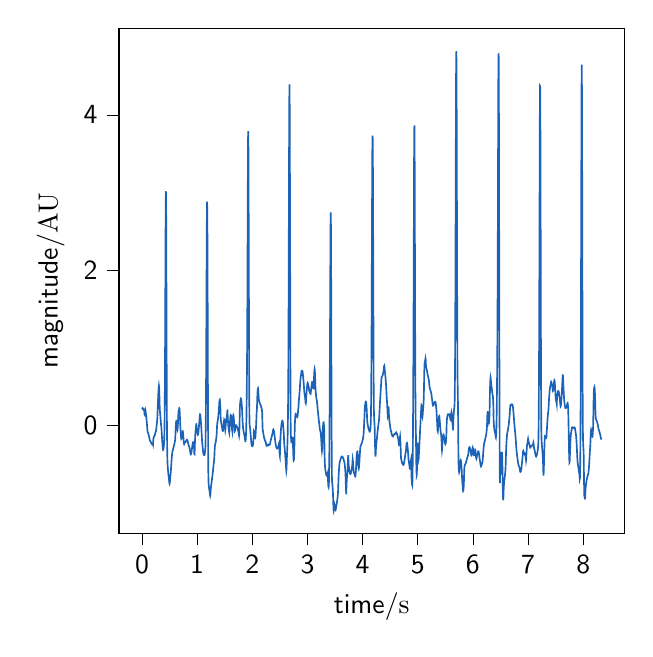
\begin{tikzpicture}
\pgfplotsset{
   every axis/.append style={
		font=\fontsize{10}{10}\sffamily},
	every non boxed x axis/.append style={
		x axis line style={->}
	},
	every non boxed y axis/.append style={
		y axis line style={->}
	},
	every non boxed z axis/.append style={
		z axis line style={->}
	}
}
\begin{axis}[
height=\figH,
tick align=outside,
tick pos=left,
width=\figW,
x grid style={white!69.0196078431373!black},
xlabel={time/$\si{\second}$},
xmin=-0.416499996185303, xmax=8.74649991989136,
xtick style={color=black},
y grid style={white!69.0196078431373!black},
ylabel={magnitude/\si{AU}},
ymin=-1.38940031528473, ymax=5.11472828388214,
ytick style={color=black},
ytick = {0, 2, 4},
yticklabels = {0, 2, 4},
xtick = {0, 1, 2, 3, 4, 5, 6, 7, 8},
xticklabels = {0, 1, 2, 3, 4, 5, 6, 7, 8},
]
\addplot [semithick, tud1b]
table {%
0 0.230540618300438
0.00333333341404796 0.23054151237011
0.00666666682809591 0.222391545772552
0.00999999977648258 0.218326240777969
0.0133333336561918 0.214269831776619
0.0166666675359011 0.214310452342033
0.0199999995529652 0.21844182908535
0.0233333334326744 0.22256638109684
0.0266666673123837 0.222591146826744
0.0299999993294477 0.218511328101158
0.0333333350718021 0.206237092614174
0.0366666652262211 0.198061063885689
0.0399999991059303 0.189876705408096
0.0433333329856396 0.17759507894516
0.0466666668653488 0.144781544804573
0.0500000007450581 0.140682101249695
0.0533333346247673 0.157105699181557
0.0566666685044765 0.165356621146202
0.0599999986588955 0.181795433163643
0.0633333325386047 0.194154590368271
0.0666666701436043 0.181915476918221
0.0700000002980232 0.157314002513885
0.0733333304524422 0.136778563261032
0.0766666680574417 0.12034098058939
0.0799999982118607 0.0998164936900139
0.0833333358168602 0.0751872733235359
0.0866666659712791 0.0464294962584972
0.0900000035762787 0.0176374204456806
0.0933333337306976 -0.0111417593434453
0.0966666638851166 -0.0440343581140041
0.100000001490116 -0.0687779560685158
0.103333331644535 -0.0771191045641899
0.106666669249535 -0.0853601023554802
0.109999999403954 -0.0895159989595413
0.113333337008953 -0.0977329611778259
0.116666667163372 -0.105982393026352
0.119999997317791 -0.118317350745201
0.123333334922791 -0.126608267426491
0.126666665077209 -0.134861305356026
0.129999995231628 -0.139037817716599
0.133333340287209 -0.151343211531639
0.136666670441628 -0.167802557349205
0.140000000596046 -0.180237308144569
0.143333330750465 -0.18854808807373
0.146666660904884 -0.192742213606834
0.150000005960464 -0.196891188621521
0.153333336114883 -0.201044395565987
0.156666666269302 -0.205196708440781
0.159999996423721 -0.20935121178627
0.16333332657814 -0.217579454183578
0.16666667163372 -0.221791312098503
0.170000001788139 -0.225947871804237
0.173333331942558 -0.230108678340912
0.176666662096977 -0.234268605709076
0.180000007152557 -0.238429725170135
0.183333337306976 -0.242593005299568
0.186666667461395 -0.242688924074173
0.189999997615814 -0.238656222820282
0.193333327770233 -0.234559804201126
0.196666672825813 -0.234526440501213
0.200000002980232 -0.242689251899719
0.203333333134651 -0.198163971304893
0.20666666328907 -0.173031195998192
0.209999993443489 -0.160447254776955
0.213333338499069 -0.152126759290695
0.216666668653488 -0.143877610564232
0.219999998807907 -0.135630160570145
0.223333328962326 -0.135491788387299
0.226666674017906 -0.131453692913055
0.230000004172325 -0.127334609627724
0.233333334326744 -0.119161985814571
0.236666664481163 -0.106844149529934
0.239999994635582 -0.0984954908490181
0.243333339691162 -0.0902313962578773
0.246666669845581 -0.0819649696350098
0.25 -0.0777443498373032
0.253333330154419 -0.0695658475160599
0.256666660308838 -0.0572386123239994
0.259999990463257 -0.0367282330989838
0.263333320617676 -0.0160157587379217
0.266666680574417 0.00874953623861074
0.270000010728836 0.0295724719762802
0.273333340883255 0.0502980276942253
0.276666671037674 0.0791166797280312
0.280000001192093 0.124325774610043
0.283333331346512 0.190142095088959
0.286666661500931 0.252505958080292
0.28999999165535 0.310724049806595
0.293333321809769 0.364797532558441
0.296666651964188 0.418791025876999
0.300000011920929 0.460684239864349
0.303333342075348 0.49821674823761
0.306666672229767 0.515455186367035
0.310000002384186 0.495814561843872
0.313333332538605 0.446880042552948
0.316666662693024 0.372921019792557
0.319999992847443 0.269981384277344
0.323333323001862 0.206491068005562
0.326666653156281 0.176462575793266
0.330000013113022 0.151437282562256
0.333333343267441 0.122487597167492
0.33666667342186 0.0934241786599159
0.340000003576279 0.0643312558531761
0.343333333730698 0.0352514535188675
0.346666663885117 0.0101743927225471
0.349999994039536 -0.0107519924640656
0.353333324193954 -0.0395986959338188
0.356666654348373 -0.072747528553009
0.360000014305115 -0.118089526891708
0.363333344459534 -0.15985731780529
0.366666674613953 -0.189442485570908
0.370000004768372 -0.22260969877243
0.373333334922791 -0.255943804979324
0.376666665077209 -0.285262107849121
0.379999995231628 -0.302396565675735
0.383333325386047 -0.311069309711456
0.386666655540466 -0.307396411895752
0.389999985694885 -0.299260646104813
0.393333345651627 -0.282946556806564
0.396666675806046 -0.262306243181229
0.400000005960464 -0.233488887548447
0.403333336114883 -0.180282741785049
0.406666666269302 -0.0779961720108986
0.409999996423721 0.0702556669712067
0.41333332657814 0.312540888786316
0.416666656732559 0.674919724464417
0.419999986886978 1.16215801239014
0.423333346843719 1.7426962852478
0.426666676998138 2.342777967453
0.430000007152557 2.83603835105896
0.433333337306976 3.01643586158752
0.436666667461395 2.97172713279724
0.439999997615814 2.55386662483215
0.443333327770233 1.82420790195465
0.446666657924652 1.01721143722534
0.449999988079071 0.350910186767578
0.453333348035812 -0.0688868835568428
0.456666678190231 -0.282490938901901
0.46000000834465 -0.411312013864517
0.463333338499069 -0.488783419132233
0.466666668653488 -0.524161636829376
0.469999998807907 -0.553673505783081
0.473333328962326 -0.583013951778412
0.476666659116745 -0.612355291843414
0.479999989271164 -0.633732974529266
0.483333319425583 -0.654737651348114
0.486666679382324 -0.671745181083679
0.490000009536743 -0.696546912193298
0.493333339691162 -0.721741795539856
0.496666669845581 -0.73897522687912
0.5 -0.747853517532349
0.503333330154419 -0.740394294261932
0.506666660308838 -0.720181941986084
0.509999990463257 -0.691392838954926
0.513333320617676 -0.666151106357574
0.516666650772095 -0.641122281551361
0.519999980926514 -0.616080284118652
0.523333311080933 -0.58705997467041
0.526666641235352 -0.553844809532166
0.529999971389771 -0.51642370223999
0.533333361148834 -0.478768080472946
0.536666691303253 -0.445103138685226
0.540000021457672 -0.415601372718811
0.543333351612091 -0.390289217233658
0.54666668176651 -0.365177810192108
0.550000011920929 -0.348012924194336
0.553333342075348 -0.331287741661072
0.556666672229767 -0.322491109371185
0.560000002384186 -0.314148902893066
0.563333332538605 -0.305798292160034
0.566666662693024 -0.297447323799133
0.569999992847443 -0.289096087217331
0.573333323001862 -0.276776224374771
0.576666653156281 -0.268184959888458
0.579999983310699 -0.259826123714447
0.583333313465118 -0.2514608502388
0.586666643619537 -0.239137023687363
0.589999973773956 -0.226570725440979
0.593333303928375 -0.214000910520554
0.596666693687439 -0.201421454548836
0.600000023841858 -0.188841551542282
0.603333353996277 -0.164393588900566
0.606666684150696 -0.107564739882946
0.610000014305115 -0.0526585020124912
0.613333344459534 -0.00593234971165657
0.616666674613953 0.0324336439371109
0.620000004768372 0.0584239587187767
0.623333334922791 0.0599730238318443
0.626666665077209 0.0402392446994781
0.629999995231628 0.0192000847309828
0.633333325386047 -0.00183465064037591
0.636666655540466 -0.0228752382099628
0.639999985694885 -0.0439268238842487
0.643333315849304 -0.053145132958889
0.646666646003723 -0.0418588034808636
0.649999976158142 -0.00557222589850426
0.653333306312561 0.0402089394629002
0.656666696071625 0.0904818773269653
0.660000026226044 0.156810820102692
0.663333356380463 0.184868887066841
0.666666686534882 0.194420352578163
0.670000016689301 0.202875182032585
0.673333346843719 0.215271010994911
0.676666676998138 0.224009051918983
0.680000007152557 0.220671951770782
0.683333337306976 0.185012668371201
0.686666667461395 0.135301426053047
0.689999997615814 0.0886297225952148
0.693333327770233 0.0264948159456253
0.696666657924652 -0.0249779149889946
0.699999988079071 -0.0638475641608238
0.70333331823349 -0.097898043692112
0.706666648387909 -0.131682723760605
0.709999978542328 -0.157618403434753
0.713333308696747 -0.171205058693886
0.716666638851166 -0.168198853731155
0.720000028610229 -0.156154379248619
0.723333358764648 -0.139581009745598
0.726666688919067 -0.126619219779968
0.730000019073486 -0.110046438872814
0.733333349227905 -0.089237853884697
0.736666679382324 -0.0720401406288147
0.740000009536743 -0.0708113685250282
0.743333339691162 -0.0864852964878082
0.746666669845581 -0.111241981387138
0.75 -0.140546411275864
0.753333330154419 -0.166252195835114
0.756666660308838 -0.199482291936874
0.759999990463257 -0.229428917169571
0.763333320617676 -0.235621154308319
0.766666650772095 -0.228154107928276
0.769999980926514 -0.223632708191872
0.773333311080933 -0.219430565834045
0.776666641235352 -0.219134226441383
0.779999971389771 -0.215259075164795
0.783333361148834 -0.211053967475891
0.786666691303253 -0.210752159357071
0.790000021457672 -0.206877335906029
0.793333351612091 -0.206572771072388
0.79666668176651 -0.202699393033981
0.800000011920929 -0.198490649461746
0.803333342075348 -0.190381854772568
0.806666672229767 -0.189727008342743
0.810000002384186 -0.18585430085659
0.813333332538605 -0.189434602856636
0.816666662693024 -0.189805626869202
0.819999992847443 -0.185937494039536
0.823333323001862 -0.189507886767387
0.826666653156281 -0.193776488304138
0.829999983310699 -0.201938077807426
0.833333313465118 -0.214344471693039
0.836666643619537 -0.223211780190468
0.839999973773956 -0.235623493790627
0.843333303928375 -0.244499236345291
0.846666693687439 -0.253026962280273
0.850000023841858 -0.261554956436157
0.853333353996277 -0.270083278417587
0.856666684150696 -0.274730205535889
0.860000014305115 -0.282901585102081
0.863333344459534 -0.291436284780502
0.866666674613953 -0.29997330904007
0.870000004768372 -0.316271811723709
0.873333334922791 -0.329442083835602
0.876666665077209 -0.346112430095673
0.879999995231628 -0.35929349064827
0.883333325386047 -0.364344090223312
0.886666655540466 -0.368646174669266
0.889999985694885 -0.365201652050018
0.893333315849304 -0.357121706008911
0.896666646003723 -0.344793111085892
0.899999976158142 -0.32820263504982
0.903333306312561 -0.31122824549675
0.906666696071625 -0.294249147176743
0.910000026226044 -0.277257084846497
0.913333356380463 -0.260268688201904
0.916666686534882 -0.239404127001762
0.920000016689301 -0.225882560014725
0.923333346843719 -0.213132157921791
0.926666676998138 -0.211975529789925
0.930000007152557 -0.212004631757736
0.933333337306976 -0.223618596792221
0.936666667461395 -0.240295737981796
0.939999997615814 -0.261233597993851
0.943333327770233 -0.28258940577507
0.946666657924652 -0.315516233444214
0.949999988079071 -0.36894902586937
0.95333331823349 -0.3704514503479
0.956666648387909 -0.296828925609589
0.959999978542328 -0.227417692542076
0.963333308696747 -0.166891187429428
0.966666638851166 -0.118732422590256
0.970000028610229 -0.0833685323596001
0.973333358764648 -0.0607850030064583
0.976666688919067 -0.0355933308601379
0.980000019073486 -0.00614621583372355
0.983333349227905 0.0160474125295877
0.986666679382324 0.0181666426360607
0.990000009536743 -0.0087573230266571
0.993333339691162 -0.0424984022974968
0.996666669845581 -0.0613003186881542
1 -0.0745573192834854
1.00333333015442 -0.0912221148610115
1.00666666030884 -0.104494147002697
1.00999999046326 -0.113492026925087
1.01333332061768 -0.118217118084431
1.01666665077209 -0.114833526313305
1.01999998092651 -0.102899320423603
1.02333331108093 -0.0824151411652565
1.02666664123535 -0.0610332861542702
1.02999997138977 -0.0358218662440777
1.03333330154419 -0.00632060971111059
1.03666663169861 0.0197882372885942
1.03999996185303 0.0493083111941814
1.04333329200745 0.0792786255478859
1.04666662216187 0.109242491424084
1.04999995231628 0.131573393940926
1.0533332824707 0.145347952842712
1.05666661262512 0.142910033464432
1.05999994277954 0.127166092395782
1.06333339214325 0.102408342063427
1.06666672229767 0.0690683126449585
1.07000005245209 0.0348045863211155
1.07333338260651 0.000514745712280273
1.07666671276093 -0.0375882834196091
1.08000004291534 -0.076166532933712
1.08333337306976 -0.118583209812641
1.08666670322418 -0.161459639668465
1.0900000333786 -0.200562849640846
1.09333336353302 -0.231562152504921
1.09666669368744 -0.253986984491348
1.10000002384186 -0.275468707084656
1.10333335399628 -0.300773680210114
1.1066666841507 -0.326564520597458
1.11000001430511 -0.348551243543625
1.11333334445953 -0.362435311079025
1.11666667461395 -0.371559023857117
1.12000000476837 -0.376387029886246
1.12333333492279 -0.376927077770233
1.12666666507721 -0.37697845697403
1.12999999523163 -0.377029836177826
1.13333332538605 -0.377081215381622
1.13666665554047 -0.369527220726013
1.13999998569489 -0.353382498025894
1.1433333158493 -0.3286372423172
1.14666664600372 -0.3028963804245
1.14999997615814 -0.280940622091293
1.15333330631256 -0.175953909754753
1.15666663646698 0.0312988385558128
1.1599999666214 0.330312192440033
1.16333329677582 0.727262377738953
1.16666662693024 1.22332215309143
1.16999995708466 1.78811061382294
1.17333328723907 2.33401727676392
1.17666661739349 2.72498774528503
1.17999994754791 2.88324761390686
1.18333327770233 2.79685306549072
1.18666660785675 2.46510314941406
1.19000005722046 1.83485054969788
1.19333338737488 1.07288217544556
1.1966667175293 0.298068106174469
1.20000004768372 -0.341296494007111
1.20333337783813 -0.628709614276886
1.20666670799255 -0.722671270370483
1.21000003814697 -0.765784084796906
1.21333336830139 -0.789547085762024
1.21666669845581 -0.807430803775787
1.22000002861023 -0.821008861064911
1.22333335876465 -0.834056735038757
1.22666668891907 -0.85088050365448
1.23000001907349 -0.872018933296204
1.23333334922791 -0.893711924552917
1.23666667938232 -0.90407931804657
1.24000000953674 -0.893975555896759
1.24333333969116 -0.862296104431152
1.24666666984558 -0.820353388786316
1.25 -0.792371153831482
1.25333333015442 -0.774110436439514
1.25666666030884 -0.756947696208954
1.25999999046326 -0.743542075157166
1.26333332061768 -0.723159909248352
1.26666665077209 -0.705427289009094
1.26999998092651 -0.684479355812073
1.27333331108093 -0.666729271411896
1.27666664123535 -0.645772457122803
1.27999997138977 -0.628018617630005
1.28333330154419 -0.607049942016602
1.28666663169861 -0.585521221160889
1.28999996185303 -0.56022447347641
1.29333329200745 -0.538115382194519
1.29666662216187 -0.512808561325073
1.29999995231628 -0.494436919689178
1.3033332824707 -0.477199196815491
1.30666661262512 -0.456204801797867
1.30999994277954 -0.434635162353516
1.31333339214325 -0.390567034482956
1.31666672229767 -0.327997595071793
1.32000005245209 -0.281870245933533
1.32333338260651 -0.257341802120209
1.32666671276093 -0.243216276168823
1.33000004291534 -0.234005749225616
1.33333337306976 -0.22537237405777
1.33666670322418 -0.212996020913124
1.3400000333786 -0.200030162930489
1.34333336353302 -0.183316990733147
1.34666669368744 -0.166010856628418
1.35000002384186 -0.144952073693275
1.35333335399628 -0.115833811461926
1.3566666841507 -0.0780281499028206
1.36000001430511 -0.0203349366784096
1.36333334445953 0.0216812286525965
1.36666667461395 0.0383279100060463
1.37000000476837 0.0513435304164886
1.37333333492279 0.0606344491243362
1.37666666507721 0.0767781585454941
1.37999999523163 0.0941470414400101
1.38333332538605 0.115243978798389
1.38666665554047 0.144417628645897
1.38999998569489 0.178544819355011
1.3933333158493 0.209579795598984
1.39666664600372 0.236275285482407
1.39999997615814 0.269819885492325
1.40333330631256 0.308310210704803
1.40666663646698 0.332568496465683
1.4099999666214 0.335738062858582
1.41333329677582 0.320905685424805
1.41666662693024 0.292415589094162
1.41999995708466 0.258319616317749
1.42333328723907 0.193851754069328
1.42666661739349 0.10945250838995
1.42999994754791 0.0707945227622986
1.43333327770233 0.0514953508973122
1.43666660785675 0.0378236658871174
1.44000005722046 0.0247782524675131
1.44333338737488 0.0117293260991573
1.4466667175293 -0.00131673715077341
1.45000004768372 -0.0143758747726679
1.45333337783813 -0.0274321492761374
1.45666670799255 -0.0442008376121521
1.46000003814697 -0.0616172552108765
1.46333336830139 -0.0679320469498634
1.46666669845581 -0.0685930699110031
1.47000002861023 -0.0574983209371567
1.47333335876465 -0.0370417907834053
1.47666668891907 -0.0115582216531038
1.48000001907349 0.00717562297359109
1.48333334922791 0.0357059314846992
1.48666667938232 0.0625154599547386
1.49000000953674 0.0775869712233543
1.49333333969116 0.0722052007913589
1.49666666984558 0.0524138882756233
1.5 0.0269307680428028
1.50333333015442 0.000773031963035464
1.50666666030884 -0.0364673770964146
1.50999999046326 -0.057284239679575
1.51333332061768 -0.0415561981499195
1.51666665077209 -0.00499571114778519
1.51999998092651 0.0232159644365311
1.52333331108093 0.0457231253385544
1.52666664123535 0.0675561875104904
1.52999997138977 0.0857029631733894
1.53333330154419 0.0995029732584953
1.53666663169861 0.112614557147026
1.53999996185303 0.129412591457367
1.54333329200745 0.150577068328857
1.54666662216187 0.187151968479156
1.54999995231628 0.189732596278191
1.5533332824707 0.137609556317329
1.55666661262512 0.0874748453497887
1.55999994277954 0.0467395447194576
1.56333339214325 0.011090062558651
1.56666672229767 -0.0128803765401244
1.57000005245209 -0.0310671515762806
1.57333338260651 -0.0448969602584839
1.57666671276093 -0.0616935789585114
1.58000004291534 -0.0828683748841286
1.58333337306976 -0.0937531813979149
1.58666670322418 -0.0695373043417931
1.5900000333786 -0.0132654402405024
1.59333336353302 0.0260422024875879
1.59666669368744 0.0573885962367058
1.60000002384186 0.0880441218614578
1.60333335399628 0.115041173994541
1.6066666841507 0.130357295274734
1.61000001430511 0.136198714375496
1.61333334445953 0.133282601833344
1.61666667461395 0.121608674526215
1.62000000476837 0.104828640818596
1.62333333492279 0.0800060480833054
1.62666666507721 0.0318139269948006
1.62999999523163 -0.0244355723261833
1.63333332538605 -0.0522263422608376
1.63666665554047 -0.0668500661849976
1.63999998569489 -0.0180082488805056
1.6433333158493 0.036110732704401
1.64666664600372 0.070501334965229
1.64999997615814 0.101227566599846
1.65333330631256 0.124653570353985
1.65666663646698 0.135686278343201
1.6599999666214 0.129912659525871
1.66333329677582 0.106586374342442
1.66666662693024 0.0766276270151138
1.66999995708466 0.0422735512256622
1.67333328723907 0.0071500395424664
1.67666661739349 -0.0461803637444973
1.67999994754791 -0.0778133347630501
1.68333327770233 -0.0751053690910339
1.68666660785675 -0.0590649358928204
1.69000005722046 -0.0451319552958012
1.69333338737488 -0.0319507792592049
1.6966667175293 -0.0151425655931234
1.70000004768372 -0.0011906495783478
1.70333337783813 0.00473978510126472
1.70666670799255 0.0055102938786149
1.71000003814697 0.00188557186629623
1.71333336830139 -0.00251234555616975
1.71666669845581 -0.00691143376752734
1.72000002861023 -0.0113116921856999
1.72333335876465 -0.0157109722495079
1.72666668891907 -0.0201146490871906
1.73000001907349 -0.0281370989978313
1.73333334922791 -0.0405633635818958
1.73666667938232 -0.0501526854932308
1.74000000953674 -0.0589672103524208
1.74333333969116 -0.0641645416617393
1.74666666984558 -0.0721917301416397
1.75 -0.0810083970427513
1.75333333015442 -0.0970499739050865
1.75666666030884 -0.118296667933464
1.75999999046326 -0.129516065120697
1.76333332061768 -0.10586704313755
1.76666665077209 -0.0425579100847244
1.76999998092651 0.0567983612418175
1.77333331108093 0.187820330262184
1.77666664123535 0.256072461605072
1.77999997138977 0.290995657444
1.78333330154419 0.311099469661713
1.78666663169861 0.328776299953461
1.78999996185303 0.342870384454727
1.79333329200745 0.34895396232605
1.79666662216187 0.346214652061462
1.79999995231628 0.334652125835419
1.8033332824707 0.314260721206665
1.80666661262512 0.288646221160889
1.80999994277954 0.258592486381531
1.81333339214325 0.224131256341934
1.81666672229767 0.174473911523819
1.82000005245209 0.121507182717323
1.82333338260651 0.0685005113482475
1.82666671276093 0.0262708887457848
1.83000004291534 -0.00273014488629997
1.83333337306976 -0.0292394813150167
1.83666670322418 -0.0485869795084
1.8400000333786 -0.0626912340521812
1.84333336353302 -0.0759657770395279
1.84666669368744 -0.0892341062426567
1.85000002384186 -0.102512434124947
1.85333335399628 -0.112211771309376
1.8566666841507 -0.124655172228813
1.86000001430511 -0.134362161159515
1.86333334445953 -0.14680315554142
1.86666667461395 -0.167249336838722
1.87000000476837 -0.185816094279289
1.87333333492279 -0.199976623058319
1.87666666507721 -0.198992297053337
1.87999999523163 -0.183878824114799
1.88333332538605 -0.151908919215202
1.88666665554047 -0.105790376663208
1.88999998569489 -0.0321369767189026
1.8933333158493 0.0797228366136551
1.89666664600372 0.249246999621391
1.89999997615814 0.448725640773773
1.90333330631256 0.695336282253265
1.90666663646698 1.03094017505646
1.9099999666214 1.48900234699249
1.91333329677582 2.06830143928528
1.91666662693024 2.71073055267334
1.91999995708466 3.31684041023254
1.92333328723907 3.70855212211609
1.92666661739349 3.79099559783936
1.92999994754791 3.57819652557373
1.93333327770233 2.99884510040283
1.93666660785675 2.20393419265747
1.94000005722046 1.37787640094757
1.94333338737488 0.673416495323181
1.9466667175293 0.201221525669098
1.95000004768372 0.0349679738283157
1.95333337783813 -0.00328135280869901
1.95666670799255 -0.0183992832899094
1.96000003814697 -0.0317261666059494
1.96333336830139 -0.0556849874556065
1.96666669845581 -0.0823417603969574
1.97000002861023 -0.116103887557983
1.97333335876465 -0.148120164871216
1.97666668891907 -0.175710216164589
1.98000001907349 -0.202396854758263
1.98333334922791 -0.225559011101723
1.98666667938232 -0.244273453950882
1.99000000953674 -0.255025625228882
1.99333333969116 -0.260418802499771
1.99666666984558 -0.264898806810379
2 -0.26585054397583
2.00333333015442 -0.265885561704636
2.00666666030884 -0.262391209602356
2.00999999046326 -0.254444569349289
2.01333332061768 -0.238526701927185
2.01666665077209 -0.217225968837738
2.01999998092651 -0.187942922115326
2.02333331108093 -0.156799405813217
2.02666664123535 -0.100991427898407
2.02999997138977 -0.0668405741453171
2.03333330154419 -0.0718128010630608
2.03666663169861 -0.0992764830589294
2.03999996185303 -0.119906835258007
2.04333329200745 -0.134228974580765
2.04666662216187 -0.147613450884819
2.04999995231628 -0.157486781477928
2.0533332824707 -0.159395098686218
2.05666661262512 -0.145362362265587
2.05999994277954 -0.113494098186493
2.06333327293396 -0.0743393748998642
2.06666660308838 -0.0341973640024662
2.0699999332428 0.0129410484805703
2.07333326339722 0.0725542977452278
2.07666659355164 0.135031446814537
2.07999992370605 0.17646649479866
2.08333325386047 0.208690777420998
2.08666658401489 0.264503329992294
2.08999991416931 0.348017960786819
2.09333324432373 0.412854254245758
2.09666657447815 0.449949622154236
2.09999990463257 0.474279165267944
2.10333323478699 0.479178845882416
2.10666656494141 0.461754500865936
2.10999989509583 0.428994178771973
2.11333322525024 0.396805763244629
2.11666655540466 0.362081408500671
2.11999988555908 0.336844891309738
2.1233332157135 0.318040072917938
2.1266667842865 0.303689062595367
2.13000011444092 0.297295331954956
2.13333344459534 0.292863428592682
2.13666677474976 0.288428127765656
2.14000010490417 0.280508249998093
2.14333343505859 0.275082588195801
2.14666676521301 0.27064648270607
2.15000009536743 0.269688576459885
2.15333342552185 0.262759894132614
2.15666675567627 0.253844410181046
2.16000008583069 0.244924381375313
2.16333341598511 0.236004203557968
2.16666674613953 0.227081686258316
2.17000007629395 0.218152433633804
2.17333340644836 0.205750405788422
2.17666673660278 0.188868805766106
2.1800000667572 0.150148943066597
2.18333339691162 0.0463288873434067
2.18666672706604 -0.0295187067240477
2.19000005722046 -0.0610434487462044
2.19333338737488 -0.0730550065636635
2.1966667175293 -0.0854944586753845
2.20000004768372 -0.0989565253257751
2.20333337783813 -0.11242537945509
2.20666670799255 -0.125887885689735
2.21000003814697 -0.13936048746109
2.21333336830139 -0.152833312749863
2.21666669845581 -0.162855163216591
2.22000002861023 -0.168389201164246
2.22333335876465 -0.176355361938477
2.22666668891907 -0.185355007648468
2.23000001907349 -0.194352582097054
2.23333334922791 -0.199904561042786
2.23666667938232 -0.20442071557045
2.24000000953674 -0.205484747886658
2.24333333969116 -0.208961948752403
2.24666666984558 -0.220380544662476
2.25 -0.233883202075958
2.25333333015442 -0.247395977377892
2.25666666030884 -0.257458955049515
2.25999999046326 -0.259588688611984
2.26333332061768 -0.256179243326187
2.26666665077209 -0.255159854888916
2.26999998092651 -0.255193054676056
2.27333331108093 -0.255226314067841
2.27666664123535 -0.255259543657303
2.27999997138977 -0.251853853464127
2.28333330154419 -0.247389495372772
2.28666663169861 -0.242921710014343
2.28999996185303 -0.241890832781792
2.29333329200745 -0.245356380939484
2.29666662216187 -0.246455490589142
2.29999995231628 -0.249920308589935
2.3033332824707 -0.247591435909271
2.30666661262512 -0.246551617980003
2.30999994277954 -0.246583700180054
2.31333327293396 -0.246615752577782
2.31666660308838 -0.243221595883369
2.3199999332428 -0.238748505711555
2.32333326339722 -0.230851531028748
2.32666659355164 -0.218449920415878
2.32999992370605 -0.201537534594536
2.33333325386047 -0.190379172563553
2.33666658401489 -0.181386455893517
2.33999991416931 -0.172397956252098
2.34333324432373 -0.163400530815125
2.34666657447815 -0.154407382011414
2.34999990463257 -0.145405262708664
2.35333323478699 -0.136403024196625
2.35666656494141 -0.12740284204483
2.35999989509583 -0.118395909667015
2.36333322525024 -0.109386652708054
2.36666655540466 -0.0969685912132263
2.36999988555908 -0.0800327360630035
2.3733332157135 -0.068803682923317
2.3766667842865 -0.0597832798957825
2.38000011444092 -0.0507627539336681
2.38333344459534 -0.0485439524054527
2.38666677474976 -0.0553551912307739
2.39000010490417 -0.0643941611051559
2.39333343505859 -0.0734376832842827
2.39666676521301 -0.0858763009309769
2.40000009536743 -0.10284461826086
2.40333342552185 -0.124332241714001
2.40666675567627 -0.143547266721725
2.41000008583069 -0.165036901831627
2.41333341598511 -0.18427100777626
2.41666674613953 -0.202381610870361
2.42000007629395 -0.217105433344841
2.42333340644836 -0.230695471167564
2.42666673660278 -0.247687950730324
2.4300000667572 -0.259035050868988
2.43333339691162 -0.268119990825653
2.43666672706604 -0.277205049991608
2.44000005722046 -0.286288052797318
2.44333338737488 -0.29199543595314
2.4466667175293 -0.293178498744965
2.45000004768372 -0.293216407299042
2.45333337783813 -0.293254315853119
2.45666670799255 -0.293292224407196
2.46000003814697 -0.286578774452209
2.46333336830139 -0.280931055545807
2.46666669845581 -0.276435822248459
2.47000002861023 -0.271941602230072
2.47333335876465 -0.264074325561523
2.47666668891907 -0.258415192365646
2.48000001907349 -0.247171357274055
2.48333334922791 -0.226872220635414
2.48666667938232 -0.221072122454643
2.49000000953674 -0.264862775802612
2.49333333969116 -0.323839455842972
2.49666666984558 -0.382845669984818
2.5 -0.394782572984695
2.50333333015442 -0.329771369695663
2.50666666030884 -0.250363051891327
2.50999999046326 -0.183309495449066
2.51333332061768 -0.126537278294563
2.51666665077209 -0.0821421816945076
2.51999998092651 -0.0480159297585487
2.52333331108093 -0.0229550488293171
2.52666664123535 -0.000253018457442522
2.52999997138977 0.0191066283732653
2.53333330154419 0.0372733324766159
2.53666663169861 0.0487442873418331
2.53999996185303 0.0578350350260735
2.54333329200745 0.0635837018489838
2.54666662216187 0.0647882223129272
2.54999995231628 0.0581060126423836
2.5533332824707 0.0456775315105915
2.55666661262512 0.0253623202443123
2.55999994277954 -0.000710805878043175
2.56333327293396 -0.0280021857470274
2.56666660308838 -0.0586202591657639
2.5699999332428 -0.0904680714011192
2.57333326339722 -0.139002218842506
2.57666659355164 -0.193604126572609
2.57999992370605 -0.234894543886185
2.58333325386047 -0.264664351940155
2.58666658401489 -0.292007565498352
2.58999991416931 -0.3160140812397
2.59333324432373 -0.345485508441925
2.59666657447815 -0.37740296125412
2.59999990463257 -0.409320801496506
2.60333323478699 -0.441246867179871
2.60666656494141 -0.476514875888824
2.60999989509583 -0.513012290000916
2.61333322525024 -0.556185901165009
2.61666655540466 -0.581877827644348
2.61999988555908 -0.563647329807281
2.6233332157135 -0.501949429512024
2.6266667842865 -0.435698300600052
2.63000011444092 -0.365324079990387
2.63333344459534 -0.299047231674194
2.63666677474976 -0.245187029242516
2.64000010490417 -0.168574199080467
2.64333343505859 -0.0620297156274319
2.64666676521301 0.114894948899746
2.65000009536743 0.352079838514328
2.65333342552185 0.705701053142548
2.65666675567627 1.23049700260162
2.66000008583069 1.92831563949585
2.66333341598511 2.7352979183197
2.66666674613953 3.51350831985474
2.67000007629395 4.10344266891479
2.67333340644836 4.39121723175049
2.67666673660278 4.29769802093506
2.6800000667572 3.80552911758423
2.68333339691162 2.99198961257935
2.68666672706604 2.00143265724182
2.69000005722046 1.03284597396851
2.69333338737488 0.278251469135284
2.6966667175293 -0.0437776781618595
2.70000004768372 -0.131080448627472
2.70333337783813 -0.171515256166458
2.70666670799255 -0.201529964804649
2.71000003814697 -0.21584153175354
2.71333336830139 -0.215148761868477
2.71666669845581 -0.210604161024094
2.72000002861023 -0.202770471572876
2.72333335876465 -0.193645358085632
2.72666668891907 -0.181236922740936
2.73000001907349 -0.157689213752747
2.73333334922791 -0.159771680831909
2.73666667938232 -0.229262948036194
2.74000000953674 -0.301192551851273
2.74333333969116 -0.365353375673294
2.74666666984558 -0.419669032096863
2.75 -0.450443118810654
2.75333333015442 -0.447210788726807
2.75666666030884 -0.413902640342712
2.75999999046326 -0.359620809555054
2.76333332061768 -0.283738434314728
2.76666665077209 -0.142492920160294
2.76999998092651 -0.0232400931417942
2.77333331108093 0.041678462177515
2.77666664123535 0.0855857506394386
2.77999997138977 0.123600788414478
2.78333330154419 0.143975585699081
2.78666663169861 0.151231810450554
2.78999996185303 0.149316504597664
2.79333329200745 0.144746601581573
2.79666662216187 0.143436193466187
2.79999995231628 0.140197902917862
2.8033332824707 0.135626226663589
2.80666661262512 0.131053358316422
2.80999994277954 0.12322710454464
2.81333327293396 0.114060133695602
2.81666660308838 0.111394658684731
2.8199999332428 0.117906779050827
2.82333326339722 0.136852771043777
2.82666659355164 0.159838616847992
2.82999992370605 0.186077162623405
2.83333325386047 0.210418239235878
2.83666658401489 0.236666530370712
2.83999991416931 0.267516404390335
2.84333324432373 0.306202441453934
2.84666657447815 0.34113410115242
2.84999990463257 0.370114862918854
2.85333323478699 0.397745430469513
2.85666656494141 0.422153115272522
2.85999989509583 0.454912424087524
2.86333322525024 0.491771280765533
2.86666655540466 0.528621554374695
2.86999988555908 0.565508127212524
2.8733332157135 0.595917522907257
2.8766667842865 0.617154598236084
2.88000011444092 0.63240909576416
2.88333344459534 0.649526834487915
2.88666677474976 0.671252071857452
2.89000010490417 0.691136360168457
2.89333343505859 0.703194856643677
2.89666676521301 0.706051290035248
2.90000009536743 0.706140995025635
2.90333342552185 0.706230700016022
2.90666675567627 0.706320464611053
2.91000008583069 0.699975371360779
2.91333341598511 0.687629818916321
2.91666674613953 0.667541265487671
2.92000007629395 0.641559720039368
2.92333340644836 0.614159643650055
2.92666673660278 0.589869558811188
2.9300000667572 0.567031681537628
2.93333339691162 0.538116991519928
2.93666672706604 0.50310617685318
2.94000005722046 0.463537156581879
2.94333338737488 0.43117168545723
2.9466667175293 0.409560143947601
2.95000004768372 0.394150972366333
2.95333337783813 0.380447894334793
2.95666670799255 0.366741299629211
2.96000003814697 0.344673156738281
2.96333336830139 0.314438581466675
2.96666669845581 0.29052996635437
2.97000002861023 0.28567835688591
2.97333335876465 0.306263476610184
2.97666668891907 0.346304148435593
2.98000001907349 0.389642953872681
2.98333334922791 0.420747399330139
2.98666667938232 0.44630229473114
2.99000000953674 0.473896622657776
2.99333333969116 0.501511454582214
2.99666666984558 0.529126524925232
3 0.547132134437561
3.00333333015442 0.551644265651703
3.00666666030884 0.547033429145813
3.00999999046326 0.535606265068054
3.01333332061768 0.524160504341125
3.01666665077209 0.517281174659729
3.01999998092651 0.510537981987
3.02333331108093 0.49704897403717
3.02666664123535 0.478723257780075
3.02999997138977 0.460379302501678
3.03333330154419 0.446218550205231
3.03666663169861 0.439128458499908
3.03999996185303 0.434584468603134
3.04333329200745 0.430039286613464
3.04666662216187 0.423537135124207
3.04999995231628 0.416309297084808
3.0533332824707 0.409869313240051
3.05666661262512 0.408158034086227
3.05999994277954 0.421073466539383
3.06333327293396 0.443133562803268
3.06666660308838 0.467286765575409
3.0699999332428 0.485773682594299
3.07333326339722 0.502552032470703
3.07666659355164 0.518104612827301
3.07999992370605 0.536600351333618
3.08333325386047 0.553488850593567
3.08666658401489 0.562670826911926
3.08999991416931 0.561201989650726
3.09333324432373 0.553646266460419
3.09666657447815 0.538416862487793
3.09999990463257 0.520040512084961
3.10333323478699 0.500248074531555
3.10666656494141 0.481389373540878
3.10999989509583 0.480309337377548
3.11333322525024 0.506716668605804
3.11666655540466 0.560587644577026
3.11999988555908 0.633241295814514
3.1233332157135 0.691582202911377
3.1266667842865 0.716980934143066
3.13000011444092 0.729770660400391
3.13333344459534 0.716276407241821
3.13666677474976 0.670465469360352
3.14000010490417 0.603116929531097
3.14333343505859 0.518011450767517
3.14666676521301 0.463981449604034
3.15000009536743 0.433622777462006
3.15333342552185 0.409653216600418
3.15666675567627 0.383771479129791
3.16000008583069 0.365342676639557
3.16333341598511 0.347730726003647
3.16666674613953 0.333902955055237
3.17000007629395 0.320081919431686
3.17333340644836 0.305516302585602
3.17666673660278 0.285658627748489
3.1800000667572 0.257951140403748
3.18333339691162 0.230229884386063
3.18666672706604 0.203100994229317
3.19000005722046 0.180004000663757
3.19333338737488 0.156889826059341
3.1966667175293 0.133775532245636
3.20000004768372 0.110655404627323
3.20333337783813 0.0875294730067253
3.20666670799255 0.0647972002625465
3.21000003814697 0.0462888218462467
3.21333336830139 0.0277757961302996
3.21666669845581 0.00894047319889069
3.22000002861023 -0.0142127703875303
3.22333335876465 -0.0371247082948685
3.22666668891907 -0.0552338324487209
3.23000001907349 -0.0643237456679344
3.23333334922791 -0.0691142603754997
3.23666667938232 -0.0785112679004669
3.24000000953674 -0.0925951227545738
3.24333333969116 -0.11583386361599
3.24666666984558 -0.143709421157837
3.25 -0.180825412273407
3.25333333015442 -0.222566872835159
3.25666666030884 -0.264330178499222
3.25999999046326 -0.301552772521973
3.26333332061768 -0.325111210346222
3.26666665077209 -0.30787456035614
3.26999998092651 -0.258086860179901
3.27333331108093 -0.184890702366829
3.27666664123535 -0.0798720940947533
3.27999997138977 -0.0299115423113108
3.28333330154419 0.00349237537011504
3.28666663169861 0.0273867938667536
3.28999996185303 0.0420592539012432
3.29333329200745 0.0432736799120903
3.29666662216187 0.026442427188158
3.29999995231628 -0.000493568833917379
3.3033332824707 -0.0408116988837719
3.30666661262512 -0.169017314910889
3.30999994277954 -0.349245846271515
3.31333327293396 -0.45018082857132
3.31666660308838 -0.502380430698395
3.3199999332428 -0.536984980106354
3.32333326339722 -0.557748734951019
3.32666659355164 -0.576411783695221
3.32999992370605 -0.591200172901154
3.33333325386047 -0.601370096206665
3.33666658401489 -0.614574372768402
3.33999991416931 -0.628606557846069
3.34333324432373 -0.638887882232666
3.34666657447815 -0.644545197486877
3.34999990463257 -0.645583391189575
3.35333323478699 -0.642000913619995
3.35666656494141 -0.637425243854523
3.35999989509583 -0.632850646972656
3.36333322525024 -0.62470668554306
3.36666655540466 -0.615467190742493
3.36999988555908 -0.658757030963898
3.3733332157135 -0.712463140487671
3.3766667842865 -0.756917774677277
3.38000011444092 -0.785323441028595
3.38333344459534 -0.791859984397888
3.38666677474976 -0.771905183792114
3.39000010490417 -0.724195241928101
3.39333343505859 -0.596252501010895
3.39666676521301 -0.359978139400482
3.40000009536743 -0.0220906510949135
3.40333342552185 0.387496590614319
3.40666675567627 0.838824331760406
3.41000008583069 1.31947469711304
3.41333341598511 1.82470989227295
3.41666674613953 2.31383180618286
3.42000007629395 2.65425324440002
3.42333340644836 2.74449157714844
3.42666673660278 2.52873706817627
3.4300000667572 1.9387024641037
3.43333339691162 1.11315381526947
3.43666672706604 0.283921450376511
3.44000005722046 -0.353565335273743
3.44333338737488 -0.646045804023743
3.4466667175293 -0.716213405132294
3.45000004768372 -0.741608738899231
3.45333337783813 -0.767752528190613
3.45666670799255 -0.79588782787323
3.46000003814697 -0.829280853271484
3.46333336830139 -0.884958207607269
3.46666669845581 -0.965432286262512
3.47000002861023 -1.03413283824921
3.47333335876465 -1.07569897174835
3.47666668891907 -1.09375810623169
3.48000001907349 -1.08396685123444
3.48333334922791 -1.058309674263
3.48666667938232 -1.03037691116333
3.49000000953674 -1.01411771774292
3.49333333969116 -1.02338910102844
3.49666666984558 -1.04464077949524
3.5 -1.06125497817993
3.50333333015442 -1.07322382926941
3.50666666030884 -1.08271884918213
3.50999999046326 -1.08579325675964
3.51333332061768 -1.07702672481537
3.51666665077209 -1.06104135513306
3.51999998092651 -1.04447841644287
3.52333331108093 -1.03054988384247
3.52666664123535 -1.01860356330872
3.52999997138977 -1.0074143409729
3.53333330154419 -0.993482828140259
3.53666663169861 -0.97766387462616
3.53999996185303 -0.959038496017456
3.54333329200745 -0.940399169921875
3.54666662216187 -0.921764314174652
3.54999995231628 -0.899625062942505
3.5533332824707 -0.868169188499451
3.55666661262512 -0.818958282470703
3.55999994277954 -0.747074246406555
3.56333327293396 -0.678555190563202
3.56666660308838 -0.628678321838379
3.5699999332428 -0.591220855712891
3.57333326339722 -0.555274844169617
3.57666659355164 -0.522492170333862
3.57999992370605 -0.494063675403595
3.58333325386047 -0.476761847734451
3.58666658401489 -0.46412393450737
3.58999991416931 -0.454790592193604
3.59333324432373 -0.446779310703278
3.59666657447815 -0.442138075828552
3.59999990463257 -0.436233282089233
3.60333323478699 -0.426894128322601
3.60666656494141 -0.418741405010223
3.60999989509583 -0.412932008504868
3.61333322525024 -0.405839681625366
3.61666655540466 -0.405889868736267
3.61999988555908 -0.404879122972488
3.6233332157135 -0.40125560760498
3.6266667842865 -0.400308638811111
3.63000011444092 -0.396618872880936
3.63333344459534 -0.397597640752792
3.63666677474976 -0.402351498603821
3.64000010490417 -0.407105386257172
3.64333343505859 -0.411861538887024
3.64666676521301 -0.415819436311722
3.65000009536743 -0.417402803897858
3.65333342552185 -0.426869571208954
3.65666675567627 -0.436336398124695
3.66000008583069 -0.44580551981926
3.66333341598511 -0.455281615257263
3.66666674613953 -0.464753031730652
3.67000007629395 -0.474231451749802
3.67333340644836 -0.484784573316574
3.67666673660278 -0.504183411598206
3.6800000667572 -0.528282999992371
3.68333339691162 -0.556618332862854
3.68666672706604 -0.585766971111298
3.69000005722046 -0.625390291213989
3.69333338737488 -0.688780665397644
3.6966667175293 -0.776913285255432
3.70000004768372 -0.841956257820129
3.70333337783813 -0.88276332616806
3.70666670799255 -0.803320050239563
3.71000003814697 -0.738248467445374
3.71333336830139 -0.696155190467834
3.71666669845581 -0.663210451602936
3.72000002861023 -0.630417585372925
3.72333335876465 -0.606890261173248
3.72666668891907 -0.583313167095184
3.73000001907349 -0.522027313709259
3.73333334922791 -0.451338976621628
3.73666667938232 -0.408533126115799
3.74000000953674 -0.379968464374542
3.74333333969116 -0.448231488466263
3.74666666984558 -0.496303617954254
3.75 -0.51640772819519
3.75333333015442 -0.53986531496048
3.75666666030884 -0.563560009002686
3.75999999046326 -0.578384220600128
3.76333332061768 -0.592639327049255
3.76666665077209 -0.602524876594543
3.76999998092651 -0.6120525598526
3.77333331108093 -0.617279529571533
3.77666664123535 -0.622084617614746
3.77999997138977 -0.622651755809784
3.78333330154419 -0.61852240562439
3.78666663169861 -0.609693706035614
3.78999996185303 -0.600308120250702
3.79333329200745 -0.586812794208527
3.79666662216187 -0.576764702796936
3.79999995231628 -0.5673668384552
3.8033332824707 -0.553964793682098
3.80666661262512 -0.539829790592194
3.80999994277954 -0.525691270828247
3.81333327293396 -0.503730118274689
3.81666660308838 -0.460726976394653
3.8199999332428 -0.428793460130692
3.82333326339722 -0.442375481128693
3.82666659355164 -0.485021501779556
3.82999992370605 -0.51747190952301
3.83333325386047 -0.549669325351715
3.83666658401489 -0.579232275485992
3.83999991416931 -0.60044538974762
3.84333324432373 -0.608630001544952
3.84666657447815 -0.613443672657013
3.84999990463257 -0.618260860443115
3.85333323478699 -0.626597583293915
3.85666656494141 -0.636158227920532
3.85999989509583 -0.642270743846893
3.86333322525024 -0.650514245033264
3.86666655540466 -0.65330696105957
3.86999988555908 -0.646679580211639
3.8733332157135 -0.62398087978363
3.8766667842865 -0.595591902732849
3.88000011444092 -0.560663461685181
3.88333344459534 -0.519537210464478
3.88666677474976 -0.457743227481842
3.89000010490417 -0.405505418777466
3.89333343505859 -0.378435879945755
3.89666676521301 -0.359477311372757
3.90000009536743 -0.343581914901733
3.90333342552185 -0.332398772239685
3.90666675567627 -0.331913828849792
3.91000008583069 -0.357410311698914
3.91333341598511 -0.404254645109177
3.91666674613953 -0.445028305053711
3.92000007629395 -0.484064698219299
3.92333340644836 -0.52126157283783
3.92666673660278 -0.546222805976868
3.9300000667572 -0.554267466068268
3.93333339691162 -0.543424010276794
3.93666672706604 -0.519078433513641
3.94000005722046 -0.485272496938705
3.94333338737488 -0.449895620346069
3.9466667175293 -0.408859938383102
3.95000004768372 -0.366452366113663
3.95333337783813 -0.330955535173416
3.95666670799255 -0.300168395042419
3.96000003814697 -0.276561051607132
3.96333336830139 -0.262417435646057
3.96666669845581 -0.255322515964508
3.97000002861023 -0.250591993331909
3.97333335876465 -0.245860323309898
3.97666668891907 -0.241125136613846
3.98000001907349 -0.234125971794128
3.98333334922791 -0.226858019828796
3.98666667938232 -0.222119957208633
3.99000000953674 -0.215216651558876
3.99333333969116 -0.205711394548416
3.99666666984558 -0.196203827857971
4 -0.186689227819443
4.003333568573 -0.179209679365158
4.00666666030884 -0.170465633273125
4.01000022888184 -0.15421062707901
4.01333332061768 -0.135152459144592
4.01666688919067 -0.114190869033337
4.01999998092651 -0.0884737148880959
4.02333354949951 -0.0470237582921982
4.02666664123535 0.0114013412967324
4.03000020980835 0.0603750087320805
4.03333330154419 0.108536779880524
4.03666687011719 0.167544424533844
4.03999996185303 0.221291333436966
4.04333353042603 0.254621028900146
4.04666662216187 0.275326669216156
4.05000019073486 0.289687097072601
4.0533332824707 0.30252081155777
4.0566668510437 0.309111505746841
4.05999994277954 0.307681947946548
4.06333351135254 0.30150580406189
4.06666660308838 0.287789642810822
4.07000017166138 0.262556552886963
4.07333326339722 0.229901507496834
4.07666683197021 0.179124712944031
4.07999992370605 0.112467102706432
4.08333349227905 0.0660512521862984
4.08666658401489 0.0397610701620579
4.09000015258789 0.0218020100146532
4.09333324432373 0.00858767051249743
4.09666681289673 -0.000983535079285502
4.09999990463257 -0.0116193424910307
4.10333347320557 -0.0249425694346428
4.10666656494141 -0.0345189869403839
4.1100001335144 -0.0431280396878719
4.11333322525024 -0.0488532818853855
4.11666679382324 -0.0584384426474571
4.11999988555908 -0.0671535953879356
4.12333345413208 -0.0711189433932304
4.12666654586792 -0.0719259455800056
4.13000011444092 -0.0751956403255463
4.13333320617676 -0.0704134255647659
4.13666677474976 -0.0642329752445221
4.1399998664856 -0.0485378913581371
4.14333343505859 -0.0233152583241463
4.14666652679443 0.0138140134513378
4.15000009536743 0.0846087038516998
4.15333318710327 0.232038885354996
4.15666675567627 0.497230648994446
4.15999984741211 0.869996964931488
4.16333341598511 1.37334942817688
4.16666650772095 1.97633075714111
4.17000007629395 2.61016821861267
4.17333316802979 3.18011808395386
4.17666673660278 3.58632922172546
4.17999982833862 3.73088097572327
4.18333339691162 3.69915628433228
4.18666648864746 3.39508199691772
4.19000005722046 2.80922961235046
4.1933331489563 2.06446170806885
4.1966667175293 1.28406643867493
4.19999980926514 0.615779519081116
4.20333337783813 0.261777132749557
4.20666646957397 0.146537825465202
4.21000003814697 0.0840032622218132
4.21333312988281 0.0453737527132034
4.21666669845581 0.0163927283138037
4.21999979019165 -0.0453284196555614
4.22333335876465 -0.173138946294785
4.22666645050049 -0.289010971784592
4.23000001907349 -0.363062530755997
4.23333311080933 -0.398707777261734
4.23666667938232 -0.373511523008347
4.23999977111816 -0.322215050458908
4.24333333969116 -0.282733887434006
4.246666431427 -0.248720049858093
4.25 -0.219474196434021
4.253333568573 -0.19935254752636
4.25666666030884 -0.180129915475845
4.26000022888184 -0.1609026491642
4.26333332061768 -0.137399882078171
4.26666688919067 -0.109124168753624
4.26999998092651 -0.0844447165727615
4.27333354949951 -0.0645371749997139
4.27666664123535 -0.0452843122184277
4.28000020980835 -0.0219274200499058
4.28333330154419 -0.00191394041758031
4.28666687011719 0.0173582080751657
4.28999996185303 0.0326312892138958
4.29333353042603 0.0470894426107407
4.29666662216187 0.065491795539856
4.30000019073486 0.0925760492682457
4.3033332824707 0.133103549480438
4.3066668510437 0.180346935987473
4.30999994277954 0.236162602901459
4.31333351135254 0.282768279314041
4.31666660308838 0.318755656480789
4.32000017166138 0.352544873952866
4.32333326339722 0.390024602413177
4.32666683197021 0.432294547557831
4.32999992370605 0.472168982028961
4.33333349227905 0.510845184326172
4.33666658401489 0.549521327018738
4.34000015258789 0.588197290897369
4.34333324432373 0.616485953330994
4.34666681289673 0.626971006393433
4.34999990463257 0.63187563419342
4.35333347320557 0.636779069900513
4.35666656494141 0.638355374336243
4.3600001335144 0.641731262207031
4.36333322525024 0.646637618541718
4.36666679382324 0.654778361320496
4.36999988555908 0.664519965648651
4.37333345413208 0.677426755428314
4.37666654586792 0.692013144493103
4.38000011444092 0.706599593162537
4.38333320617676 0.727308034896851
4.38666677474976 0.748543262481689
4.3899998664856 0.767973005771637
4.39333343505859 0.772597670555115
4.39666652679443 0.759068131446838
4.40000009536743 0.731120467185974
4.40333318710327 0.700202107429504
4.40666675567627 0.676921427249908
4.40999984741211 0.657644271850586
4.41333341598511 0.635601043701172
4.41666650772095 0.608752071857452
4.42000007629395 0.577082693576813
4.42333316802979 0.540597021579742
4.42666673660278 0.50456690788269
4.42999982833862 0.468132764101028
4.43333339691162 0.42175966501236
4.43666648864746 0.371062219142914
4.44000005722046 0.332636266946793
4.4433331489563 0.301145136356354
4.4466667175293 0.255146592855453
4.44999980926514 0.197032451629639
4.45333337783813 0.150665998458862
4.45666646957397 0.121405713260174
4.46000003814697 0.129237428307533
4.46333312988281 0.177405953407288
4.46666669845581 0.226325109601021
4.46999979019165 0.24591588973999
4.47333335876465 0.208215653896332
4.47666645050049 0.148219048976898
4.48000001907349 0.11084271222353
4.48333311080933 0.0817487314343452
4.48666667938232 0.0566799938678741
4.48999977111816 0.0392626263201237
4.49333333969116 0.0227479506283998
4.496666431427 0.00525551103055477
4.5 -0.0111908102408051
4.503333568573 -0.0306109469383955
4.50666666030884 -0.0464065112173557
4.51000022888184 -0.056121401488781
4.51333332061768 -0.065845787525177
4.51666688919067 -0.0755701139569283
4.51999998092651 -0.0852943658828735
4.52333354949951 -0.0950209498405457
4.52666664123535 -0.1063626781106
4.53000020980835 -0.117797926068306
4.53333330154419 -0.122673138976097
4.53666687011719 -0.127549529075623
4.53999996185303 -0.132425874471664
4.54333353042603 -0.135859340429306
4.54666662216187 -0.137285128235817
4.55000019073486 -0.139411926269531
4.5533332824707 -0.134566366672516
4.5566668510437 -0.129717260599136
4.55999994277954 -0.124866977334023
4.56333351135254 -0.120017945766449
4.56666660308838 -0.116371318697929
4.57000017166138 -0.116385228931904
4.57333326339722 -0.115261077880859
4.57666683197021 -0.110406160354614
4.57999992370605 -0.106621362268925
4.58333349227905 -0.106634095311165
4.58666658401489 -0.106646828353405
4.59000015258789 -0.106659561395645
4.59333324432373 -0.105737015604973
4.59666681289673 -0.100879855453968
4.59999990463257 -0.0960191413760185
4.60333347320557 -0.0919898524880409
4.60666656494141 -0.0912028849124908
4.6100001335144 -0.0878670364618301
4.61333322525024 -0.092752605676651
4.61666679382324 -0.0976381376385689
4.61999988555908 -0.102526023983955
4.62333345413208 -0.108043260872364
4.62666654586792 -0.117213882505894
4.63000011444092 -0.122667022049427
4.63333320617676 -0.132436394691467
4.63666677474976 -0.142208084464073
4.6399998664856 -0.151982098817825
4.64333343505859 -0.161760851740837
4.64666652679443 -0.17193067073822
4.65000009536743 -0.187305971980095
4.65333318710327 -0.211732596158981
4.65666675567627 -0.235310435295105
4.65999984741211 -0.244347468018532
4.66333341598511 -0.239058151841164
4.66666650772095 -0.224249765276909
4.67000007629395 -0.204746171832085
4.67333316802979 -0.184877678751945
4.67666673660278 -0.15102706849575
4.67999982833862 -0.136753678321838
4.68333339691162 -0.16127610206604
4.68666648864746 -0.219949826598167
4.69000005722046 -0.288368731737137
4.6933331489563 -0.366514682769775
4.6966667175293 -0.415983319282532
4.69999980926514 -0.431574910879135
4.70333337783813 -0.441565275192261
4.70666646957397 -0.451400518417358
4.71000003814697 -0.461240530014038
4.71333312988281 -0.471075594425201
4.71666669845581 -0.48091784119606
4.71999979019165 -0.486198216676712
4.72333335876465 -0.486621737480164
4.72666645050049 -0.491172552108765
4.73000001907349 -0.491666585206985
4.73333311080933 -0.500578224658966
4.73666667938232 -0.506037414073944
4.73999977111816 -0.506634414196014
4.74333333969116 -0.50236988067627
4.746666431427 -0.493242144584656
4.75 -0.479242205619812
4.753333568573 -0.464607775211334
4.75666666030884 -0.454152047634125
4.76000022888184 -0.440248429775238
4.76333332061768 -0.425600498914719
4.76666688919067 -0.410949140787125
4.76999998092651 -0.396290719509125
4.77333354949951 -0.377607941627502
4.77666664123535 -0.362029522657394
4.78000020980835 -0.347359955310822
4.78333330154419 -0.336609065532684
4.78666687011719 -0.31518879532814
4.78999996185303 -0.290696680545807
4.79333353042603 -0.262381345033646
4.79666662216187 -0.236766129732132
4.80000019073486 -0.223500818014145
4.8033332824707 -0.221140757203102
4.8066668510437 -0.228527754545212
4.80999994277954 -0.245667725801468
4.81333351135254 -0.265336722135544
4.81666660308838 -0.285000681877136
4.82000017166138 -0.308223485946655
4.82333326339722 -0.336329698562622
4.82666683197021 -0.372779458761215
4.82999992370605 -0.408693194389343
4.83333349227905 -0.439718842506409
4.83666658401489 -0.459129840135574
4.84000015258789 -0.473920822143555
4.84333324432373 -0.488722532987595
4.84666681289673 -0.503531336784363
4.84999990463257 -0.521575331687927
4.85333347320557 -0.541299939155579
4.85666656494141 -0.554692566394806
4.8600001335144 -0.555184900760651
4.86333322525024 -0.541027724742889
4.86666679382324 -0.518340647220612
4.86999988555908 -0.490781515836716
4.87333345413208 -0.455317497253418
4.87666654586792 -0.442697376012802
4.88000011444092 -0.488693118095398
4.88333320617676 -0.568356454372406
4.88666677474976 -0.649248719215393
4.8899998664856 -0.699815154075623
4.89333343505859 -0.729441404342651
4.89666652679443 -0.759067296981812
4.90000009536743 -0.766895771026611
4.90333318710327 -0.724854052066803
4.90666675567627 -0.600135087966919
4.90999984741211 -0.37265220284462
4.91333341598511 -0.0580693744122982
4.91666650772095 0.332689464092255
4.92000007629395 0.811810314655304
4.92333316802979 1.39884114265442
4.92666673660278 2.08629989624023
4.92999982833862 2.81157779693604
4.93333339691162 3.46015357971191
4.93666648864746 3.82821941375732
4.94000005722046 3.86288523674011
4.9433331489563 3.54433536529541
4.9466667175293 2.82989573478699
4.94999980926514 1.94839119911194
4.95333337783813 1.12281274795532
4.95666646957397 0.511890888214111
4.96000003814697 0.170356675982475
4.96333312988281 0.0123801939189434
4.96666669845581 -0.111651696264744
4.96999979019165 -0.296858638525009
4.97333335876465 -0.47963535785675
4.97666645050049 -0.576693654060364
4.98000001907349 -0.642468690872192
4.98333311080933 -0.634698987007141
4.98666667938232 -0.515237033367157
4.98999977111816 -0.370279103517532
4.99333333969116 -0.279615461826324
4.996666431427 -0.235430717468262
5 -0.238156914710999
5.003333568573 -0.310670644044876
5.00666666030884 -0.371782779693604
5.01000022888184 -0.41312974691391
5.01333332061768 -0.436883985996246
5.01666688919067 -0.424749255180359
5.01999998092651 -0.382264345884323
5.02333354949951 -0.334297567605972
5.02666664123535 -0.288391709327698
5.03000020980835 -0.240345388650894
5.03333330154419 -0.194499164819717
5.03666687011719 -0.145032703876495
5.03999996185303 -0.0968479290604591
5.04333353042603 -0.0510733313858509
5.04666662216187 -0.00156037416309118
5.05000019073486 0.0479398742318153
5.0533332824707 0.097451739013195
5.0566668510437 0.145878374576569
5.05999994277954 0.190450608730316
5.06333351135254 0.232977867126465
5.06666660308838 0.260651350021362
5.07000017166138 0.255834400653839
5.07333326339722 0.230152249336243
5.07666683197021 0.200451105833054
5.07999992370605 0.169869363307953
5.08333349227905 0.137691468000412
5.08666658401489 0.123456180095673
5.09000015258789 0.142160341143608
5.09333324432373 0.180382341146469
5.09666681289673 0.209460139274597
5.09999990463257 0.235601425170898
5.10333347320557 0.270957827568054
5.10666656494141 0.313633739948273
5.1100001335144 0.383722603321075
5.11333322525024 0.501991987228394
5.11666679382324 0.649604082107544
5.11999988555908 0.736306667327881
5.12333345413208 0.793464958667755
5.12666654586792 0.821829915046692
5.13000011444092 0.831508696079254
5.13333320617676 0.836880743503571
5.13666677474976 0.847463369369507
5.1399998664856 0.865982413291931
5.14333343505859 0.85407030582428
5.14666652679443 0.795607924461365
5.15000009536743 0.76616245508194
5.15333318710327 0.746580183506012
5.15666675567627 0.736732721328735
5.15999984741211 0.726877987384796
5.16333341598511 0.717023432254791
5.16666650772095 0.70716404914856
5.17000007629395 0.697302401065826
5.17333316802979 0.68254142999649
5.17666673660278 0.667704820632935
5.17999982833862 0.65286111831665
5.18333339691162 0.642813563346863
5.18666648864746 0.632938504219055
5.19000005722046 0.623063564300537
5.1933331489563 0.613183796405792
5.1966667175293 0.598645508289337
5.19999980926514 0.588410675525665
5.20333337783813 0.57392954826355
5.20666646957397 0.549951791763306
5.21000003814697 0.520604848861694
5.21333312988281 0.499762445688248
5.21666669845581 0.488809734582901
5.21999979019165 0.478907406330109
5.22333335876465 0.468997895717621
5.22666645050049 0.463441044092178
5.23000001907349 0.454198569059372
5.23333311080933 0.448567658662796
5.23666667938232 0.439389884471893
5.23999977111816 0.429474771022797
5.24333333969116 0.423733592033386
5.246666431427 0.410508960485458
5.25 0.391493529081345
5.253333568573 0.367523699998856
5.25666666030884 0.35070925951004
5.26000022888184 0.335793823003769
5.26333332061768 0.316898077726364
5.26666688919067 0.293037056922913
5.26999998092651 0.275932520627975
5.27333354949951 0.264864236116409
5.27666664123535 0.258747398853302
5.28000020980835 0.261381208896637
5.28333330154419 0.262640029191971
5.28666687011719 0.266399085521698
5.28999996185303 0.27142322063446
5.29333353042603 0.276447296142578
5.29666662216187 0.281472593545914
5.30000019073486 0.290090441703796
5.3033332824707 0.296556413173676
5.3066668510437 0.301588177680969
5.30999994277954 0.306619942188263
5.31333351135254 0.308199733495712
5.31666660308838 0.308235585689545
5.32000017166138 0.304890066385269
5.32333326339722 0.29658168554306
5.32666683197021 0.283301323652267
5.32999992370605 0.261781454086304
5.33333349227905 0.236808449029922
5.33666658401489 0.215044558048248
5.34000015258789 0.188720092177391
5.34333324432373 0.146157398819923
5.34666681289673 0.0992729812860489
5.34999990463257 0.0511821024119854
5.35333347320557 0.00721821002662182
5.35666656494141 -0.0357987508177757
5.3600001335144 -0.0689897462725639
5.36333322525024 -0.0764402002096176
5.36666679382324 -0.0569645687937737
5.36999988555908 -0.0183435175567865
5.37333345413208 0.0182332172989845
5.37666654586792 0.0482774376869202
5.38000011444092 0.0783360153436661
5.38333320617676 0.105678901076317
5.38666677474976 0.122673183679581
5.3899998664856 0.124750532209873
5.39333343505859 0.109283149242401
5.39666652679443 0.0816536545753479
5.40000009536743 0.0516040101647377
5.40333318710327 0.0240390412509441
5.40666675567627 -0.00349781243130565
5.40999984741211 -0.0335752032697201
5.41333341598511 -0.0612582638859749
5.41666650772095 -0.0839621052145958
5.42000007629395 -0.101692385971546
5.42333316802979 -0.119061768054962
5.42666673660278 -0.139138519763947
5.42999982833862 -0.172622263431549
5.43333339691162 -0.231604129076004
5.43666648864746 -0.286745548248291
5.44000005722046 -0.317648410797119
5.4433331489563 -0.300902903079987
5.4466667175293 -0.233869969844818
5.44999980926514 -0.188800260424614
5.45333337783813 -0.158699780702591
5.45666646957397 -0.134447872638702
5.46000003814697 -0.121317520737648
5.46333312988281 -0.113169223070145
5.46666669845581 -0.111858412623405
5.46999979019165 -0.118709072470665
5.47333335876465 -0.130549356341362
5.47666645050049 -0.145637840032578
5.48000001907349 -0.159024715423584
5.48333311080933 -0.170771211385727
5.48666667938232 -0.185869589447975
5.48999977111816 -0.202579468488693
5.49333333969116 -0.221143692731857
5.496666431427 -0.23472011089325
5.5 -0.240309923887253
5.503333568573 -0.235309824347496
5.50666666030884 -0.227449312806129
5.51000022888184 -0.210987165570259
5.51333332061768 -0.188179105520248
5.51666688919067 -0.15271483361721
5.51999998092651 -0.0882578268647194
5.52333354949951 0.00742432661354542
5.52666664123535 0.0631304830312729
5.53000020980835 0.0871196091175079
5.53333330154419 0.106133155524731
5.53666687011719 0.121246472001076
5.53999996185303 0.134216338396072
5.54333353042603 0.139269158244133
5.54666662216187 0.144320666790009
5.55000019073486 0.148404777050018
5.5533332824707 0.14842189848423
5.5566668510437 0.148439034819603
5.55999994277954 0.148456156253815
5.56333351135254 0.148473292589188
5.56666660308838 0.148490428924561
5.57000017166138 0.147746562957764
5.57333326339722 0.141999587416649
5.57666683197021 0.131240412592888
5.57999992370605 0.117433659732342
5.58333349227905 0.111787870526314
5.58666658401489 0.101710997521877
5.59000015258789 0.0905452892184258
5.59333324432373 0.0719022303819656
5.59666681289673 0.0702158957719803
5.59999990463257 0.100492350757122
5.60333347320557 0.130790680646896
5.60666656494141 0.159979075193405
5.6100001335144 0.173461392521858
5.61333322525024 0.161880329251289
5.61666679382324 0.126813843846321
5.61999988555908 0.0965391471982002
5.62333345413208 0.0664362907409668
5.62666654586792 0.0413435883820057
5.63000011444092 0.0212627779692411
5.63333320617676 0.00576580408960581
5.63666677474976 -0.0295565985143185
5.6399998664856 -0.0595024600625038
5.64333343505859 0.0213272366672754
5.64666652679443 0.0871088951826096
5.65000009536743 0.127859681844711
5.65333318710327 0.163339585065842
5.65666675567627 0.193825244903564
5.65999984741211 0.21439653635025
5.66333341598511 0.234644263982773
5.66666650772095 0.254906594753265
5.67000007629395 0.342279374599457
5.67333316802979 0.542753517627716
5.67666673660278 0.86835515499115
5.67999982833862 1.36188137531281
5.68333339691162 2.02610230445862
5.68666648864746 2.82472443580627
5.69000005722046 3.65344452857971
5.6933331489563 4.36602401733398
5.6966667175293 4.76727437973022
5.69999980926514 4.8190860748291
5.70333337783813 4.52322578430176
5.70666646957397 3.81000757217407
5.71000003814697 2.88251209259033
5.71333312988281 1.9307187795639
5.71666669845581 1.15895164012909
5.71999979019165 0.709574818611145
5.72333335876465 0.521634936332703
5.72666645050049 0.391472905874252
5.73000001907349 0.214819461107254
5.73333311080933 -0.047070324420929
5.73666667938232 -0.338120132684708
5.73999977111816 -0.50249582529068
5.74333333969116 -0.562028467655182
5.746666431427 -0.586713671684265
5.75 -0.599172532558441
5.753333568573 -0.58980667591095
5.75666666030884 -0.566899120807648
5.76000022888184 -0.537743508815765
5.76333332061768 -0.514972031116486
5.76666688919067 -0.498501867055893
5.76999998092651 -0.479586839675903
5.77333354949951 -0.463038951158524
5.77666664123535 -0.45153534412384
5.78000020980835 -0.445065259933472
5.78333330154419 -0.45083475112915
5.78666687011719 -0.468183517456055
5.78999996185303 -0.499136388301849
5.79333353042603 -0.534760057926178
5.79666662216187 -0.573852002620697
5.80000019073486 -0.621400594711304
5.8033332824707 -0.672298550605774
5.8066668510437 -0.713146507740021
5.80999994277954 -0.74548077583313
5.81333351135254 -0.77607262134552
5.81666660308838 -0.806671380996704
5.82000017166138 -0.830841422080994
5.82333326339722 -0.841753959655762
5.82666683197021 -0.83751368522644
5.82999992370605 -0.81500905752182
5.83333349227905 -0.778451204299927
5.83666658401489 -0.725693821907043
5.84000015258789 -0.634708881378174
5.84333324432373 -0.561379134654999
5.84666681289673 -0.533199191093445
5.84999990463257 -0.520875930786133
5.85333347320557 -0.510757625102997
5.85666656494141 -0.503455877304077
5.8600001335144 -0.498420834541321
5.86333322525024 -0.493387073278427
5.86666679382324 -0.488349705934525
5.86999988555908 -0.483311116695404
5.87333345413208 -0.478273868560791
5.87666654586792 -0.470622628927231
5.88000011444092 -0.460484236478806
5.88333320617676 -0.450348496437073
5.88666677474976 -0.440200448036194
5.8899998664856 -0.430060088634491
5.89333343505859 -0.422346234321594
5.89666652679443 -0.414901435375214
5.90000009536743 -0.407111406326294
5.90333318710327 -0.402057707309723
5.90666675567627 -0.394715785980225
5.90999984741211 -0.386810392141342
5.91333341598511 -0.37731546163559
5.91666650772095 -0.362051069736481
5.92000007629395 -0.344633162021637
5.92333316802979 -0.324267983436584
5.92666673660278 -0.30388817191124
5.92999982833862 -0.287589490413666
5.93333339691162 -0.27941957116127
5.93666648864746 -0.276318520307541
5.94000005722046 -0.278285682201385
5.9433331489563 -0.283424437046051
5.9466667175293 -0.290430188179016
5.94999980926514 -0.298846453428268
5.95333337783813 -0.305782675743103
5.95666646957397 -0.316036343574524
5.96000003814697 -0.329729169607162
5.96333312988281 -0.348523110151291
5.96666669845581 -0.363896280527115
5.96999979019165 -0.377656996250153
5.97333335876465 -0.384762734174728
5.97666645050049 -0.383263111114502
5.98000001907349 -0.37517637014389
5.98333311080933 -0.359884291887283
5.98666667938232 -0.343135356903076
5.98999977111816 -0.319921880960464
5.99333333969116 -0.293360501527786
5.996666431427 -0.283367276191711
6 -0.291100144386292
6.003333568573 -0.306485950946808
6.00666666030884 -0.321875184774399
6.01000022888184 -0.337260395288467
6.01333332061768 -0.353806883096695
6.01666688919067 -0.372096478939056
6.01999998092651 -0.380219727754593
6.02333354949951 -0.379220545291901
6.02666664123535 -0.374141991138458
6.03000020980835 -0.368090182542801
6.03333330154419 -0.357886373996735
6.03666687011719 -0.344987541437149
6.03999996185303 -0.317678719758987
6.04333353042603 -0.295082598924637
6.04666662216187 -0.33888378739357
6.05000019073486 -0.368159472942352
6.0533332824707 -0.387975513935089
6.0566668510437 -0.403400182723999
6.05999994277954 -0.418177902698517
6.06333351135254 -0.426638394594193
6.06666660308838 -0.420403361320496
6.07000017166138 -0.405063450336456
6.07333326339722 -0.389727592468262
6.07666683197021 -0.375318974256516
6.07999992370605 -0.36979666352272
6.08333349227905 -0.359974145889282
6.08666658401489 -0.354519486427307
6.09000015258789 -0.34429931640625
6.09333324432373 -0.334362030029297
6.09666681289673 -0.329520970582962
6.09999990463257 -0.329775393009186
6.10333347320557 -0.335134536027908
6.10666656494141 -0.345585107803345
6.1100001335144 -0.361032754182816
6.11333322525024 -0.376476347446442
6.11666679382324 -0.391968905925751
6.11999988555908 -0.41256245970726
6.12333345413208 -0.428017050027847
6.12666654586792 -0.4485864341259
6.13000011444092 -0.464126974344254
6.13333320617676 -0.4796002805233
6.13666677474976 -0.495077043771744
6.1399998664856 -0.510549664497375
6.14333343505859 -0.521106243133545
6.14666652679443 -0.526558101177216
6.15000009536743 -0.522048473358154
6.15333318710327 -0.5169637799263
6.15666675567627 -0.507092773914337
6.15999984741211 -0.501613020896912
6.16333341598511 -0.491806268692017
6.16666650772095 -0.486252844333649
6.17000007629395 -0.476518005132675
6.17333316802979 -0.46166917681694
6.17666673660278 -0.446285486221313
6.17999982833862 -0.421819061040878
6.18333339691162 -0.382639288902283
6.18666648864746 -0.350397765636444
6.19000005722046 -0.319551765918732
6.1933331489563 -0.293077111244202
6.1966667175293 -0.267353683710098
6.19999980926514 -0.245958209037781
6.20333337783813 -0.229662254452705
6.20666646957397 -0.218480169773102
6.21000003814697 -0.212413728237152
6.21333312988281 -0.20310740172863
6.21666669845581 -0.192820742726326
6.21999979019165 -0.182531744241714
6.22333335876465 -0.172240421175957
6.22666645050049 -0.161951869726181
6.23000001907349 -0.151655897498131
6.23333311080933 -0.141357600688934
6.23666667938232 -0.131062045693398
6.23999977111816 -0.116865873336792
6.24333333969116 -0.0975425466895103
6.246666431427 -0.0807365477085114
6.25 -0.0576878488063812
6.253333568573 -0.0281507484614849
6.25666666030884 0.0288234576582909
6.26000022888184 0.118018060922623
6.26333332061768 0.154161721467972
6.26666688919067 0.164501011371613
6.26999998092651 0.174847736954689
6.27333354949951 0.174585580825806
6.27666664123535 0.1414475440979
6.28000020980835 0.101899355649948
6.28333330154419 0.0726039707660675
6.28666687011719 0.04677714407444
6.28999996185303 0.034381739795208
6.29333353042603 0.0425011962652206
6.29666662216187 0.0744205564260483
6.30000019073486 0.128775477409363
6.3033332824707 0.216581806540489
6.3066668510437 0.354918032884598
6.30999994277954 0.47755354642868
6.31333351135254 0.554088711738586
6.31666660308838 0.600871443748474
6.32000017166138 0.618944704532623
6.32333326339722 0.603196501731873
6.32666683197021 0.569257020950317
6.32999992370605 0.538968086242676
6.33333349227905 0.518933653831482
6.33666658401489 0.503464818000793
6.34000015258789 0.488000065088272
6.34333324432373 0.472524255514145
6.34666681289673 0.454298406839371
6.34999990463257 0.433647394180298
6.35333347320557 0.415654897689819
6.35666656494141 0.400163948535919
6.3600001335144 0.384677141904831
6.36333322525024 0.364037036895752
6.36666679382324 0.330597817897797
6.36999988555908 0.266736924648285
6.37333345413208 0.154085025191307
6.37666654586792 0.0529683157801628
6.38000011444092 0.0102695152163506
6.38333320617676 -0.0132988383993506
6.38666677474976 -0.0340381152927876
6.3899998664856 -0.0525030754506588
6.39333343505859 -0.0680581405758858
6.39666652679443 -0.0792132690548897
6.40000009536743 -0.086573913693428
6.40333318710327 -0.0969583243131638
6.40666675567627 -0.109441667795181
6.40999984741211 -0.127080589532852
6.41333341598511 -0.145817935466766
6.41666650772095 -0.153452947735786
6.42000007629395 -0.134615257382393
6.42333316802979 -0.0873538702726364
6.42666673660278 -0.0133794900029898
6.42999982833862 0.101517014205456
6.43333339691162 0.269069701433182
6.43666648864746 0.504564344882965
6.44000005722046 0.771406888961792
6.4433331489563 1.1031848192215
6.4466667175293 1.54467678070068
6.44999980926514 2.13724827766418
6.45333337783813 2.87717461585999
6.45666646957397 3.67783784866333
6.46000003814697 4.37394380569458
6.46333312988281 4.77417945861816
6.46666669845581 4.77670001983643
6.46999979019165 4.41781425476074
6.47333335876465 3.48371338844299
6.47666645050049 2.25557446479797
6.48000001907349 1.00500845909119
6.48333311080933 -0.0234700366854668
6.48666667938232 -0.632600247859955
6.48999977111816 -0.738715469837189
6.49333333969116 -0.638290107250214
6.496666431427 -0.426621526479721
6.5 -0.342992424964905
6.503333568573 -0.440949559211731
6.50666666030884 -0.5514275431633
6.51000022888184 -0.62768965959549
6.51333332061768 -0.610942184925079
6.51666688919067 -0.519977927207947
6.51999998092651 -0.441920399665833
6.52333354949951 -0.369634985923767
6.52666664123535 -0.339083790779114
6.53000020980835 -0.376386821269989
6.53333330154419 -0.456541389226913
6.53666687011719 -0.587779998779297
6.53999996185303 -0.753299713134766
6.54333353042603 -0.867789268493652
6.54666662216187 -0.936287403106689
6.55000019073486 -0.959657788276672
6.5533332824707 -0.909859538078308
6.5566668510437 -0.834518134593964
6.55999994277954 -0.788548111915588
6.56333351135254 -0.752890765666962
6.56666660308838 -0.727259576320648
6.57000017166138 -0.706159472465515
6.57333326339722 -0.680432736873627
6.57666683197021 -0.659889578819275
6.57999992370605 -0.644093096256256
6.58333349227905 -0.623130798339844
6.58666658401489 -0.597103476524353
6.59000015258789 -0.570582866668701
6.59333324432373 -0.518171906471252
6.59666681289673 -0.439844161272049
6.59999990463257 -0.345903247594833
6.60333347320557 -0.283228635787964
6.60666656494141 -0.236100688576698
6.6100001335144 -0.199388489127159
6.61333322525024 -0.16795888543129
6.61666679382324 -0.136630147695541
6.61999988555908 -0.115349158644676
6.62333345413208 -0.0944590643048286
6.62666654586792 -0.0785285383462906
6.63000011444092 -0.0726936385035515
6.63333320617676 -0.057708065956831
6.63666677474976 -0.0468831025063992
6.6399998664856 -0.0316136963665485
6.64333343505859 -0.0159295462071896
6.64666652679443 -0.000249621458351612
6.65000009536743 0.0201447363942862
6.65333318710327 0.0410605557262897
6.65666675567627 0.0666209980845451
6.65999984741211 0.0927890539169312
6.66333341598511 0.118962913751602
6.66666650772095 0.145113602280617
6.67000007629395 0.184729442000389
6.67333316802979 0.222093641757965
6.67666673660278 0.254259705543518
6.67999982833862 0.263758778572083
6.68333339691162 0.264621615409851
6.68666648864746 0.264592230319977
6.69000005722046 0.264562785625458
6.6933331489563 0.268756449222565
6.6966667175293 0.2697674036026
6.69999980926514 0.273887574672699
6.70333337783813 0.274969696998596
6.70666646957397 0.274939090013504
6.71000003814697 0.27087014913559
6.71333312988281 0.269617348909378
6.71666669845581 0.269587337970734
6.71999979019165 0.261699140071869
6.72333335876465 0.247339323163033
6.72666645050049 0.231652766466141
6.73000001907349 0.208319455385208
6.73333311080933 0.182203680276871
6.73666667938232 0.15609373152256
6.73999977111816 0.129963919520378
6.74333333969116 0.0965318381786346
6.746666431427 0.0636203587055206
6.75 0.0323042273521423
6.753333568573 0.00456581823527813
6.75666666030884 -0.0215197429060936
6.76000022888184 -0.0475994870066643
6.76333332061768 -0.0702269598841667
6.76666688919067 -0.0944775491952896
6.76999998092651 -0.120540425181389
6.77333354949951 -0.149932578206062
6.77666664123535 -0.181181609630585
6.78000020980835 -0.212454408407211
6.78333330154419 -0.246913269162178
6.78666687011719 -0.283350229263306
6.78999996185303 -0.31351226568222
6.79333353042603 -0.336405009031296
6.79666662216187 -0.357217788696289
6.80000019073486 -0.378005504608154
6.8033332824707 -0.398788571357727
6.8066668510437 -0.416619658470154
6.80999994277954 -0.435117602348328
6.81333351135254 -0.452996969223022
6.81666660308838 -0.468573689460754
6.82000017166138 -0.481313616037369
6.82333326339722 -0.494452446699142
6.82666683197021 -0.507265865802765
6.82999992370605 -0.514905512332916
6.83333349227905 -0.520051598548889
6.83666658401489 -0.525196552276611
6.84000015258789 -0.530340313911438
6.84333324432373 -0.538040399551392
6.84666681289673 -0.550906777381897
6.84999990463257 -0.566447377204895
6.85333347320557 -0.581976890563965
6.85666656494141 -0.592686653137207
6.8600001335144 -0.595439672470093
6.86333322525024 -0.593034565448761
6.86666679382324 -0.590072870254517
6.86999988555908 -0.587740421295166
6.87333345413208 -0.580252647399902
6.87666654586792 -0.567596077919006
6.88000011444092 -0.547629356384277
6.88333320617676 -0.521606266498566
6.88666677474976 -0.495576143264771
6.8899998664856 -0.471610009670258
6.89333343505859 -0.45078456401825
6.89666652679443 -0.429953515529633
6.90000009536743 -0.405272722244263
6.90333318710327 -0.374094069004059
6.90666675567627 -0.34663313627243
6.90999984741211 -0.329487383365631
6.91333341598511 -0.324441939592361
6.91666650772095 -0.331352412700653
6.92000007629395 -0.33997043967247
6.92333316802979 -0.345120280981064
6.92666673660278 -0.348623991012573
6.92999982833862 -0.348584920167923
6.93333339691162 -0.350119024515152
6.93666648864746 -0.356797605752945
6.94000005722046 -0.36712259054184
6.9433331489563 -0.375992298126221
6.9466667175293 -0.3811314702034
6.94999980926514 -0.386271983385086
6.95333337783813 -0.39275923371315
6.95666646957397 -0.404394060373306
6.96000003814697 -0.423729777336121
6.96333312988281 -0.44606676697731
6.96666669845581 -0.428764075040817
6.96999979019165 -0.374104052782059
6.97333335876465 -0.328582227230072
6.97666645050049 -0.289311021566391
6.98000001907349 -0.260343581438065
6.98333311080933 -0.24164591729641
6.98666667938232 -0.231270104646683
6.98999977111816 -0.219947353005409
6.99333333969116 -0.202568426728249
6.996666431427 -0.178425565361977
7 -0.167092204093933
7.003333568573 -0.179034113883972
7.00666666030884 -0.198161154985428
7.01000022888184 -0.208479434251785
7.01333332061768 -0.218108803033829
7.01666688919067 -0.223917007446289
7.01999998092651 -0.234228894114494
7.02333354949951 -0.243956312537193
7.02666664123535 -0.249645248055458
7.03000020980835 -0.259955823421478
7.03333330154419 -0.270269155502319
7.03666687011719 -0.280127912759781
7.03999996185303 -0.284857451915741
7.04333353042603 -0.284457057714462
7.04666662216187 -0.278925865888596
7.05000019073486 -0.268859952688217
7.0533332824707 -0.263664424419403
7.0566668510437 -0.25869607925415
7.05999994277954 -0.258666932582855
7.06333351135254 -0.25863778591156
7.06666660308838 -0.258608669042587
7.07000017166138 -0.258498340845108
7.07333326339722 -0.253353118896484
7.07666683197021 -0.253329664468765
7.07999992370605 -0.258464246988297
7.08333349227905 -0.258463025093079
7.08666658401489 -0.258433908224106
7.09000015258789 -0.243232563138008
7.09333324432373 -0.227737918496132
7.09666681289673 -0.217221900820732
7.09999990463257 -0.22666984796524
7.10333347320557 -0.256599873304367
7.10666656494141 -0.282619386911392
7.1100001335144 -0.29385632276535
7.11333322525024 -0.299330234527588
7.11666679382324 -0.309212118387222
7.11999988555908 -0.319489538669586
7.12333345413208 -0.334443897008896
7.12666654586792 -0.345210134983063
7.13000011444092 -0.360084772109985
7.13333320617676 -0.370919108390808
7.13666677474976 -0.381178677082062
7.1399998664856 -0.386928886175156
7.14333343505859 -0.392034769058228
7.14666652679443 -0.39713442325592
7.15000009536743 -0.39344722032547
7.15333318710327 -0.388257503509521
7.15666675567627 -0.383066415786743
7.15999984741211 -0.373585045337677
7.16333341598511 -0.363260835409164
7.16666650772095 -0.35292375087738
7.17000007629395 -0.338423013687134
7.17333316802979 -0.322951853275299
7.17666673660278 -0.30747652053833
7.17999982833862 -0.283895492553711
7.18333339691162 -0.262180626392365
7.18666648864746 -0.209628790616989
7.19000005722046 -0.0806147456169128
7.1933331489563 0.166543543338776
7.1966667175293 0.521833837032318
7.19999980926514 1.03277015686035
7.20333337783813 1.70932519435883
7.20666646957397 2.51574325561523
7.21000003814697 3.34878993034363
7.21333312988281 4.05106496810913
7.21666669845581 4.36928272247314
7.21999979019165 4.36490964889526
7.22333335876465 3.92295575141907
7.22666645050049 3.06006336212158
7.23000001907349 1.99100470542908
7.23333311080933 0.983895123004913
7.23666667938232 0.264709055423737
7.23999977111816 -0.0629097446799278
7.24333333969116 -0.168360665440559
7.246666431427 -0.213248774409294
7.25 -0.245806381106377
7.253333568573 -0.273296862840652
7.25666666030884 -0.305388808250427
7.26000022888184 -0.334855914115906
7.26333332061768 -0.363617897033691
7.26666688919067 -0.4037084877491
7.26999998092651 -0.455953180789948
7.27333354949951 -0.521404027938843
7.27666664123535 -0.60218358039856
7.28000020980835 -0.641634166240692
7.28333330154419 -0.605551958084106
7.28666687011719 -0.533059239387512
7.28999996185303 -0.450448453426361
7.29333353042603 -0.354763269424438
7.29666662216187 -0.266245067119598
7.30000019073486 -0.200449407100677
7.3033332824707 -0.154976472258568
7.3066668510437 -0.137916386127472
7.30999994277954 -0.140549063682556
7.31333351135254 -0.14304019510746
7.31666660308838 -0.143023952841759
7.32000017166138 -0.145546942949295
7.32333326339722 -0.148144841194153
7.32666683197021 -0.150596216320992
7.32999992370605 -0.15326339006424
7.33333349227905 -0.138862669467926
7.33666658401489 -0.103448592126369
7.34000015258789 -0.062534973025322
7.34333324432373 -0.023878701031208
7.34666681289673 0.0119049921631813
7.34999990463257 0.0476981475949287
7.35333347320557 0.0835007578134537
7.35666656494141 0.117100983858109
7.3600001335144 0.143546164035797
7.36333322525024 0.163974523544312
7.36666679382324 0.184398263692856
7.36999988555908 0.210799098014832
7.37333345413208 0.252426773309708
7.37666654586792 0.29963356256485
7.38000011444092 0.342334121465683
7.38333320617676 0.382719695568085
7.38666677474976 0.411485821008682
7.3899998664856 0.436959028244019
7.39333343505859 0.460704326629639
7.39666652679443 0.481063306331635
7.40000009536743 0.498079657554626
7.40333318710327 0.508231282234192
7.40666675567627 0.518375635147095
7.40999984741211 0.530080676078796
7.41333341598511 0.545335054397583
7.41666650772095 0.559083640575409
7.42000007629395 0.566303133964539
7.42333316802979 0.563394784927368
7.42666673660278 0.551751255989075
7.42999982833862 0.537733554840088
7.43333339691162 0.527474284172058
7.43666648864746 0.51722240447998
7.44000005722046 0.50447154045105
7.4433331489563 0.484045147895813
7.4466667175293 0.463603377342224
7.44999980926514 0.447706073522568
7.45333337783813 0.450954288244247
7.45666646957397 0.467252135276794
7.46000003814697 0.488592863082886
7.46333312988281 0.513014018535614
7.46666669845581 0.533318042755127
7.46999979019165 0.553637444972992
7.47333335876465 0.573055982589722
7.47666645050049 0.585711479187012
7.48000001907349 0.582390904426575
7.48333311080933 0.559646010398865
7.48666667938232 0.523213803768158
7.48999977111816 0.483129441738129
7.49333333969116 0.446153849363327
7.496666431427 0.400944530963898
7.5 0.361993372440338
7.503333568573 0.337643623352051
7.50666666030884 0.322879105806351
7.51000022888184 0.313158541917801
7.51333332061768 0.307130217552185
7.51666688919067 0.291431874036789
7.51999998092651 0.276826858520508
7.52333354949951 0.331641495227814
7.52666664123535 0.371015578508377
7.53000020980835 0.391301512718201
7.53333330154419 0.411332964897156
7.53666687011719 0.426328867673874
7.53999996185303 0.43626594543457
7.54333353042603 0.441295772790909
7.54666662216187 0.446224540472031
7.55000019073486 0.446111053228378
7.5533332824707 0.440981984138489
7.5566668510437 0.435854017734528
7.55999994277954 0.420588463544846
7.56333351135254 0.405326426029205
7.56666660308838 0.385049551725388
7.57000017166138 0.369665294885635
7.57333326339722 0.349484473466873
7.57666683197021 0.334027945995331
7.57999992370605 0.309074223041534
7.58333349227905 0.278873860836029
7.58666658401489 0.2579645216465
7.59000015258789 0.247133404016495
7.59333324432373 0.251084119081497
7.59666681289673 0.274812251329422
7.59999990463257 0.300117701292038
7.60333347320557 0.330013155937195
7.60666656494141 0.36040261387825
7.6100001335144 0.404352456331253
7.61333322525024 0.449891686439514
7.61666679382324 0.490988701581955
7.61999988555908 0.535859942436218
7.62333345413208 0.581390798091888
7.62666654586792 0.631281614303589
7.63000011444092 0.660279870033264
7.63333320617676 0.634243905544281
7.63666677474976 0.577541530132294
7.6399998664856 0.525123655796051
7.64333343505859 0.474464952945709
7.64666652679443 0.423768073320389
7.65000009536743 0.381338953971863
7.65333318710327 0.340810507535934
7.65666675567627 0.316361904144287
7.65999984741211 0.296097785234451
7.66333341598511 0.275818467140198
7.66666650772095 0.259470522403717
7.67000007629395 0.244282573461533
7.67333316802979 0.232919543981552
7.67666673660278 0.226590752601624
7.67999982833862 0.225279599428177
7.68333339691162 0.2252536714077
7.68666648864746 0.22892564535141
7.69000005722046 0.230290830135345
7.6933331489563 0.233891785144806
7.6966667175293 0.238917917013168
7.69999980926514 0.247494965791702
7.70333337783813 0.257570207118988
7.70666646957397 0.267638146877289
7.71000003814697 0.277708739042282
7.71333312988281 0.287781953811646
7.71666669845581 0.291090339422226
7.71999979019165 0.281040847301483
7.72333335876465 0.252649247646332
7.72666645050049 0.207480370998383
7.73000001907349 0.137584626674652
7.73333311080933 0.0216427259147167
7.73666667938232 -0.10511376708746
7.73999977111816 -0.235442847013474
7.74333333969116 -0.350061535835266
7.746666431427 -0.429519772529602
7.75 -0.473881781101227
7.753333568573 -0.468278169631958
7.75666666030884 -0.417382121086121
7.76000022888184 -0.354698479175568
7.76333332061768 -0.288410604000092
7.76666688919067 -0.22348615527153
7.76999998092651 -0.168587774038315
7.77333354949951 -0.132034569978714
7.77666664123535 -0.109556593000889
7.78000020980835 -0.0920950323343277
7.78333330154419 -0.0796258598566055
7.78666687011719 -0.0669143944978714
7.78999996185303 -0.0518038682639599
7.79333353042603 -0.0366894081234932
7.79666662216187 -0.0241036489605904
7.80000019073486 -0.0189965553581715
7.8033332824707 -0.0189943611621857
7.8066668510437 -0.0214026663452387
7.80999994277954 -0.0240578688681126
7.81333351135254 -0.0240550916641951
7.81666660308838 -0.0240523107349873
7.82000017166138 -0.0240495316684246
7.82333326339722 -0.0262827202677727
7.82666683197021 -0.0313050821423531
7.82999992370605 -0.0341699570417404
7.83333349227905 -0.034166008234024
7.83666658401489 -0.032070517539978
7.84000015258789 -0.0270363204181194
7.84333324432373 -0.0240300763398409
7.84666681289673 -0.0260118432343006
7.84999990463257 -0.0349419601261616
7.85333347320557 -0.050007589161396
7.85666656494141 -0.0650771409273148
7.8600001335144 -0.0801357850432396
7.86333322525024 -0.0951983630657196
7.86666679382324 -0.110250040888786
7.86999988555908 -0.128789976239204
7.87333345413208 -0.155589789152145
7.87666654586792 -0.188999891281128
7.88000011444092 -0.229166075587273
7.88333320617676 -0.270877987146378
7.88666677474976 -0.320704817771912
7.8899998664856 -0.377873808145523
7.89333343505859 -0.423521518707275
7.89666652679443 -0.45567587018013
7.90000009536743 -0.479292392730713
7.90333318710327 -0.49930477142334
7.90666675567627 -0.516614377498627
7.90999984741211 -0.527900457382202
7.91333341598511 -0.544154703617096
7.91666650772095 -0.562907636165619
7.92000007629395 -0.577884554862976
7.92333316802979 -0.592850565910339
7.92666673660278 -0.60782790184021
7.92999982833862 -0.624990046024323
7.93333339691162 -0.653157234191895
7.93666648864746 -0.684932112693787
7.94000005722046 -0.673905253410339
7.9433331489563 -0.598544120788574
7.9466667175293 -0.410239934921265
7.94999980926514 -0.0759477689862251
7.95333337783813 0.399699330329895
7.95666646957397 1.05093765258789
7.96000003814697 1.87894427776337
7.96333312988281 2.82327890396118
7.96666669845581 3.73455047607422
7.96999979019165 4.40784454345703
7.97333335876465 4.64683246612549
7.97666645050049 4.34068822860718
7.98000001907349 3.52603197097778
7.98333311080933 2.40352773666382
7.98666667938232 1.24579012393951
7.98999977111816 0.348885118961334
7.99333333969116 -0.0557321608066559
7.996666431427 -0.185964852571487
8 -0.258017063140869
8.00333309173584 -0.292642056941986
8.006667137146 -0.327880829572678
8.01000022888184 -0.451931774616241
8.01333332061768 -0.651471018791199
8.01666641235352 -0.841431260108948
8.02000045776367 -0.904759049415588
8.02333354949951 -0.91952645778656
8.02666664123535 -0.929415166378021
8.02999973297119 -0.939198553562164
8.03333377838135 -0.93902051448822
8.03666687011719 -0.903955101966858
8.03999996185303 -0.839086472988129
8.04333305358887 -0.803670346736908
8.04666709899902 -0.783346235752106
8.05000019073486 -0.758425652980804
8.0533332824707 -0.738221883773804
8.05666637420654 -0.722966551780701
8.0600004196167 -0.707920730113983
8.06333351135254 -0.692863643169403
8.06666660308838 -0.682504296302795
8.06999969482422 -0.67245876789093
8.07333374023438 -0.662400841712952
8.07666683197021 -0.652355015277863
8.07999992370605 -0.642306625843048
8.08333301544189 -0.636765718460083
8.08666706085205 -0.631711363792419
8.09000015258789 -0.622217774391174
8.09333324432373 -0.607776939868927
8.09666633605957 -0.59275621175766
8.10000038146973 -0.569089233875275
8.10333347320557 -0.539803981781006
8.10666656494141 -0.505607664585114
8.10999965667725 -0.470699310302734
8.1133337020874 -0.427385985851288
8.11666679382324 -0.382540315389633
8.11999988555908 -0.337705135345459
8.12333297729492 -0.305084556341171
8.12666702270508 -0.275195568799973
8.13000011444092 -0.225244760513306
8.13333320617676 -0.150592640042305
8.1366662979126 -0.0985444486141205
8.14000034332275 -0.0694029182195663
8.14333343505859 -0.0522461161017418
8.14666652679443 -0.0603254400193691
8.14999961853027 -0.0790305808186531
8.15333366394043 -0.0989245474338531
8.15666675567627 -0.11878452450037
8.15999984741211 -0.134975492954254
8.16333293914795 -0.142556443810463
8.16666698455811 -0.143886402249336
8.17000007629395 -0.129510492086411
8.17333316802979 -0.0989675372838974
8.17666625976562 -0.0571567788720131
8.18000030517578 0.0119354361668229
8.18333339691162 0.136227518320084
8.18666648864746 0.290505796670914
8.1899995803833 0.405510395765305
8.19333362579346 0.453014701604843
8.1966667175293 0.477778434753418
8.19999980926514 0.492747485637665
8.20333290100098 0.499382525682449
8.20666694641113 0.488287955522537
8.21000003814697 0.449386805295944
8.21333312988281 0.393473565578461
8.21666622161865 0.318412184715271
8.22000026702881 0.215615391731262
8.22333335876465 0.137833788990974
8.22666645050049 0.104191154241562
8.22999954223633 0.0902451425790787
8.23333358764648 0.0803157687187195
8.23666667938232 0.0703935921192169
8.23999977111816 0.0661632642149925
8.243332862854 0.0633427649736404
8.24666690826416 0.0583806931972504
8.25 0.0506710484623909
8.25333309173584 0.0407581552863121
8.256667137146 0.033515278249979
8.26000022888184 0.0259135738015175
8.26333332061768 0.0134106352925301
8.26666641235352 0.00111520499922335
8.27000045776367 -0.0113234454765916
8.27333354949951 -0.0261793863028288
8.27666664123535 -0.0385632216930389
8.27999973297119 -0.0484612137079239
8.28333377838135 -0.0559642948210239
8.28666687011719 -0.060907818377018
8.28999996185303 -0.0681740641593933
8.29333305358887 -0.0780590623617172
8.29666709899902 -0.0879465937614441
8.30000019073486 -0.0978269353508949
8.3033332824707 -0.105528093874454
8.30666637420654 -0.112614586949348
8.3100004196167 -0.122488543391228
8.31333351135254 -0.134436577558517
8.31666660308838 -0.147213220596313
8.31999969482422 -0.157084465026855
8.32333374023438 -0.166953414678574
8.32666683197021 -0.174880668520927
8.32999992370605 -0.179802626371384
};
\end{axis}

\end{tikzpicture}

        \caption{Different augmentations applied to ECG signal of the 2017 PhysioNet/CinC Challenge dataset \cite{Clifford2017}. Random reasmple aug. inspired by 2D random elastic aug. \cite{Simard2003}.}
        \label{fig:ecg_aug_3}
    \end{figure}
\end{frame}

\subsection{Training \& Validation}
\begin{frame}{Method}
\framesubtitle{Training \& Validation}
    \begin{block}{Training loss (weighted cross entropy loss)}
        $$\mathcal{L} = -\frac{1}{N}\sum_{j=1}^{N}\sum_{i=1}^{4}\alpha_{i}\,y_{ji}\,\log(\hat{y}_{ji})$$
    \end{block}
    \pause
    \begin{block}{Validation metrics (accuracy \& F1)}
        $$\operatorname{ACC}=\frac{1}{n}\sum_{j=1}^{n}\delta\left(\arg\max(\mathbf{y}_{j}), \arg\max(\hat{\mathbf{y}}_{j})\right),\quad \operatorname{F1}=\frac{1}{4}\sum_{i=1}^{4}\frac{2\text{TP}_{i}}{2\text{TP}_{i} + \text{FP}_{i} + \text{FN}_{i}}$$
    \end{block}
\end{frame}

    \section{Experiments} \label{sec:experiments}

We conduct experiments on the 2017 PhysioNet/CinC Challenge dataset \cite{Clifford2017} (Sec. \ref{subsec:physionet_dataset}). We performed three training runs (if not stated different) for each model with different random seeds, where the best run, based on the validation accuracy, was reported. Additional results can be found in the appendix.

\subsection{2017 PhysioNet/CinC Challenge Dataset} \label{subsec:physionet_dataset}

We utilize 2017 PhysioNet/CinC Challenge dataset \cite{Clifford2017} for training. The dataset includes $8529$ publicly available\footnote{\url{https://physionet.org/content/challenge-2017}} labeled single-lead ECG sequences. Each ECG sequence includes between $2714$ and $18286$ samples, recorded with a sampling frequency of $300$. For each sequence, a ground truth classification label is provided. Four classes are given, namely, normal, indicating a normal cardiac rhythm, AF, indicating atrial fibrillation, other, for different rhythms, and noisy, for a noisy measurement. Each class includes $5050$ (normal), $2456$ (AF), $738$ (other), and $284$ (noisy) samples, respectively. Visualizations of multiple sequences and corresponding labels are provided in the appendix. \\
\indent We split the data once randomly into a training and validation set. The training set includes $7000$ samples and the validation set $1528$ samples. We omit the use of $k$-fold cross-validation due to the computational expensiveness of each training run \cite{Bishop2006, Goodfellow2016}. All sequences are zero-padded, respectively, cropped to a fixed length of $18000$ samples. For a detailed description of the preprocessing see Section \ref{subsec:preprocessing}.

\subsection{Icentia$11$k dataset} \label{subsec:icentia11k_dataset}

The Icentia$11$k dataset \cite{Tan2019}, used for pre-training, consists single-lead ECG recordings of $11\si{\kilo}$ patients. The dataset is partly labeled with six different heart rhythms including atrial fibrillation. Each of the $550\si{\kilo}$ dataset sample is a sequences of approximately $1\si{\hour}$ with a sampling frequency of $250$. We resample the ECG signal to match the sampling frequency of the PhysioNet dataset. Finally, we randomly crop each sequence to a random length of $9000$ to $18000$ samples. For unlabeled crops we utilize a dummy class. For validation we split the dataset patient-wise. The resulting training set includes $10\si{\kilo}$ patients and the validation set $1\si{\kilo}$ patients.

\subsection{Results} \label{subsec:results}

Our archived classification results are presented in Table \ref{tab:results}, in which we present both the accuracy (Eq. \ref{eq:acc}) and the F1 score (Eq. \ref{eq:f1}). Table \ref{tab:results} also includes classification results of Zihlmann \etal \cite{Zihlmann2017}. The models trained by Zihlmann et al. are, however, trained on the full publicly available 2017 PhysioNet/CinC Challenge dataset and tested on the private test dataset \cite{Zihlmann2017}. Whereas our models are trained on a custom split of the publically available samples (Sec. \ref{subsec:physionet_dataset}). Additionally, the reported F1 scores by Zihlmann \etal are computed over three classes (excluding the noise class) and thus are not directly comparable to our F1 scores.

\begin{table}[h!]
    \centering
    \caption{Classification results of our proposed approaches and baselines on the 2017 PhysioNet validation set.}
    \begin{tabular}{>{\raggedright\arraybackslash}p{0.425\columnwidth}>{\raggedright\arraybackslash}p{0.1\columnwidth}>{\raggedright\arraybackslash}p{0.1\columnwidth}>{\raggedleft\arraybackslash}p{0.175\columnwidth}}
    \hline
	Model & ACC $\uparrow$ & F1 $\uparrow$ & \# Parameters\\
	\hline
	CNN baseline\textsuperscript{*} \cite{Zihlmann2017} & $0.812$ & $0.790$\textsuperscript{\dag} & $\sim 3.5\si{\mega}$ \\
	CRNN baseline\textsuperscript{*} \cite{Zihlmann2017} & $0.823$ & $0.792$\textsuperscript{\dag} & $\sim 3.5\si{\mega}$ \\
	\hline
	ECG-DualNet S & $0.8527$ & $0.8049$ & $1.8\si{\mega}$ \\
	ECG-DualNet M & $0.8560$ & $0.7938$ & $4.3\si{\mega}$ \\
	ECG-DualNet L & $0.8514$ & $0.8038$ & $6.2\si{\mega}$ \\
	ECG-DualNet XL & $\mathbf{0.8612}$ & $\mathbf{0.8164}$ & $20.7\si{\mega}$ \\
	\hline
	ECG-DualNet++ S & $0.8174$ & $0.7291$ & $1.8\si{\mega}$ \\
	ECG-DualNet++ M & $0.8259$ & $0.7730$ & $2.6\si{\mega}$ \\
	ECG-DualNet++ L & $0.8449$ & $0.7859$ & $3.7\si{\mega}$ \\
	ECG-DualNet++ XL & $\mathit{0.8593}$ & $\mathit{0.8051}$ & $8.2\si{\mega}$ \\
	ECG-DualNet++ $130\si{\mega}$ & $0.8534$ & $0.7963$ & $128\si{\mega}$ \\
	\hline
	\multicolumn{4}{l}{\textsuperscript{*} Reported literature values (private PhysioNet test set utilized).}\\
	\multicolumn{4}{l}{\textsuperscript{\dag} F1 score computed over three classes, thus not directly comparable.}
\end{tabular}

    \label{tab:results}
\end{table}

Although training was performed with fewer data samples, all ECG-DualNet architectures outperformed the baselines from the literature in classification accuracy. We observe that larger network configurations tend to perform stronger compared to smaller configurations. Especially, ECG-DualNet++ profits from a larger network capacity.\\
Training on the Icentia$11$k dataset \cite{Tan2019} yield the results presented in Table \ref{tab:results_Icentia11k}. Only two models were trained on the Icentia$11$k dataset due to the immense computational requirements.

\begin{table}[!ht]
    \centering
    \caption{Classification results of our proposed approaches on the Icentia$11$k validation set. Only a single training for each model run was conducted.}
    \begin{tabular}{>{\raggedright\arraybackslash}p{0.37\columnwidth}>{\raggedright\arraybackslash}p{0.23833\columnwidth}>{\raggedright\arraybackslash}p{0.23833\columnwidth}}
    \hline
	Model & ACC $\uparrow$ & F1 $\uparrow$ \\
	\hline
	ECG-DualNet XL & $0.8989$ & $0.4564$ \\
	ECG-DualNet++ XL & $0.8899$ & $0.4970$ \\
	\hline
\end{tabular}

    \label{tab:results_Icentia11k}
\end{table}

Using the model weights trained on the Icentia$11$k dataset (Tab. \ref{tab:results_Icentia11k}) for training on the PhysioNet dataset lead to the results presented in Table \ref{tab:full_pretraining_results}. Compared to the results, using no pre-trained weights (Tab. \ref{tab:full_results}), the results, with pre-trained weights, lead to similar or slightly worse results.

\begin{table}[!ht]
    \centering
    \caption{Classification results of our proposed approaches on the 2017 PhysioNet validation set and pre-trained on the Icentia$11$k dataset. Differences to values in Tab. \ref{tab:results} in red.}
    \begin{tabular}{>{\raggedright\arraybackslash}p{0.53\columnwidth}>{\raggedright\arraybackslash}p{0.15833\columnwidth}>{\raggedright\arraybackslash}p{0.15833\columnwidth}}
    \hline
	Model & ACC $\uparrow$ & F1 $\uparrow$ \\
	\hline
	ECG-DualNet XL & $0.8468$ \small{\textcolor{red}{$(\downarrow 0.0144)$}} & $0.8014$ \small{\textcolor{red}{$(\downarrow 0.0150)$}} \\
	ECG-DualNet++ XL & $0.8481$ \small{\textcolor{red}{$(\downarrow 0.0112)$}} & $0.7817$ \small{\textcolor{red}{$(\downarrow 0.0234)$}} \\
	\hline
\end{tabular}

    \label{tab:pretraining_results}
\end{table}

Additional experimental results of each training run are presented in the appendix.

\subsection{Ablation Study} \label{subsec:ablations}

We conducted multiple ablation training runs to investigate the effectiveness of each of the proposed components. In the presented results in table \ref{tab:ablations}, we omit one core component of our approach in each training run. We only perform ablations with one network configuration, namely ECG-DualNet M. This is due to the large computational requirements for each training run.

\begin{table}[h!]
    \centering
    \caption{Classification results on the 2017 PhysioNet validation for different ablations. ECG-DualNet L configuration utilized.}
    \begin{tabular}{>{\centering\arraybackslash}p{0.175\columnwidth}>{\centering\arraybackslash}p{0.15\columnwidth}>{\centering\arraybackslash}p{0.2\columnwidth}>{\raggedright\arraybackslash}p{0.1\columnwidth}>{\raggedright\arraybackslash}p{0.1\columnwidth}}
    \hline
	Data aug. \& dropout  & Signal encoder & Spectrogram encoder & \textcolor{white}{---} ACC $\uparrow$ & \textcolor{white}{-------} F1 $\uparrow$ \\
	\hline
	\xmark & \cmark & \cmark & $0.8272$ & $0.7493$ \\
	\cmark & \xmark & \cmark & $0.8440$ & $0.7855$ \\
	\cmark & \cmark & \xmark & $0.7264$ & $0.5813$ \\
	\cmark & \cmark & \cmark & $\mathbf{0.8560}$ & $\mathbf{0.7938}$ \\
	\hline
\end{tabular}
    \label{tab:ablations}
\end{table}

When utilizing no data augmentation (Sec. \ref{subsec:data_augmentation}) and dropout the training loss is minimized to approximately zero. This indicates signs of overfitting, even though the achieved accuracy is $0.8272$.\\
\indent From the results in table 1, it can be observed that each main component is required to reach the best classification performance. The largest impact on the classification accuracy has the spectrogram encoder. The use of data augmentation and a signal encoder has a lesser impact on the performance. 

    \section{Conclusion \& Discussion}
\begin{frame}{Conclusion \& Discussion}
    \textbf{Achievements}
    \begin{itemize}
        \item Presented the novel ECG-DualNet for ECG classification
        \item Proposed an advanced augmentation pipeline
        \item Performed extensive testing (against various beelines) including pre-training
    \end{itemize}
    \pause
    \textbf{Observations}
    \begin{itemize}
        \item Highly overparameterized models (ECG-DualNet++ $130\si{\mega}$) does not overfit in the classical sense $\to$ Deep Double Descent \cite{Nakkiran2020} ?
        \item Spectrogram encoder is the most crucial part of ECG-DualNet
        \item Extensive pre-training on the Icentia$11\si{\kilo}$ does not lead to performance benefits on the target 2017 PhysioNet dataset
    \end{itemize}
\end{frame}
    
    % Reference slide
    \begin{frame}[allowframebreaks]{References}
        % Set bib style
        \bibliographystyle{apalike}
        \bibliography{references}
    \end{frame}
    
    % Final slide
    \begin{frame}[c]{Code availability \& Questions}
        \begin{center}
            \begin{large}
                \textbf{Code, weights, and paper are available at:}
                \href{https://github.com/ChristophReich1996/ECG_Classification}{github.com/ChristophReich1996/ECG\_Classification}
            \end{large}
        \end{center}
        \begin{columns}
            \column{0.5\linewidth}
                \centering
                \includegraphics[height=4cm]{artwork/qr-code.png}
            \column{0.5\linewidth}
                \centering
                \includegraphics[height=4cm]{artwork/paper.png}
        \end{columns} 
    \end{frame}
    
    % Include appendix
    \begin{frame}{Challenge Submission}
\framesubtitle{Backup}
    \begin{itemize}
        \item ECG-DualNet XL utilized
        \item Pre-training on Icentia$11\si{\kilo}$
        \item Optimized training ($8000$ samples) and validation ($528$ samples) split used
    \end{itemize}
    \begin{table}[!ht]
        \centering
        \caption{Classification results of ECG-DualNet XL pre-trained on the Icentia$11$k dataset and fine-tuned on the PhysioNet dataset with optimized submission split. Metric computed on the small validation set. Four class results on the top and two class results below.}
        \input{table/results_challenge}
        \label{tab:results_challenge}
    \end{table}
    \begin{center}
        \hspace{-0.15cm}\begin{tabular}{>{\raggedright\arraybackslash}p{0.53\columnwidth}>{\raggedright\arraybackslash}p{0.15833\columnwidth}>{\raggedright\arraybackslash}p{0.15833\columnwidth}}
    \hline
	Model & ACC $\uparrow$ & F1 $\uparrow$ \\
	\hline
	ECG-DualNet XL ($4$ class) & $0.8840$ & $0.8549$ \\
	\hline
\end{tabular}

    \end{center}
\end{frame}

\begin{frame}{Deep Double Decent}
\framesubtitle{Backup}
    \begin{figure}[!ht]
        \centering
        \vspace{-0.2cm}
        \includegraphics[width=0.6\textwidth]{artwork/deep_double_decent.png}
        \vspace{-0.2cm}
        \caption{Illustration of the deep double decent phenomenon in image classification (CIFAR-10 \& 15\% label noise). Image taken from \cite{Nakkiran2020}.}
        \label{fig:ddd}
    \end{figure}
\end{frame}

\end{document}
